\chapter{Sviluppo}

Lo scopo di questo capitolo è quello di fornire una soluzione progettuale al problema mostrato nel capitolo precedente. Verranno quindi trattate le problematiche affrontate durante la fase di trasformazione del progetto in un artefatto eseguibile ed infine offerta una valutazione complessiva del sistema prodotto, illustrando preventivamente le informazioni relative alle metriche di valutazione utilizzate e alla natura dei test condotti.

\section{Progettazione}

\begin{figure}[h]
\centering
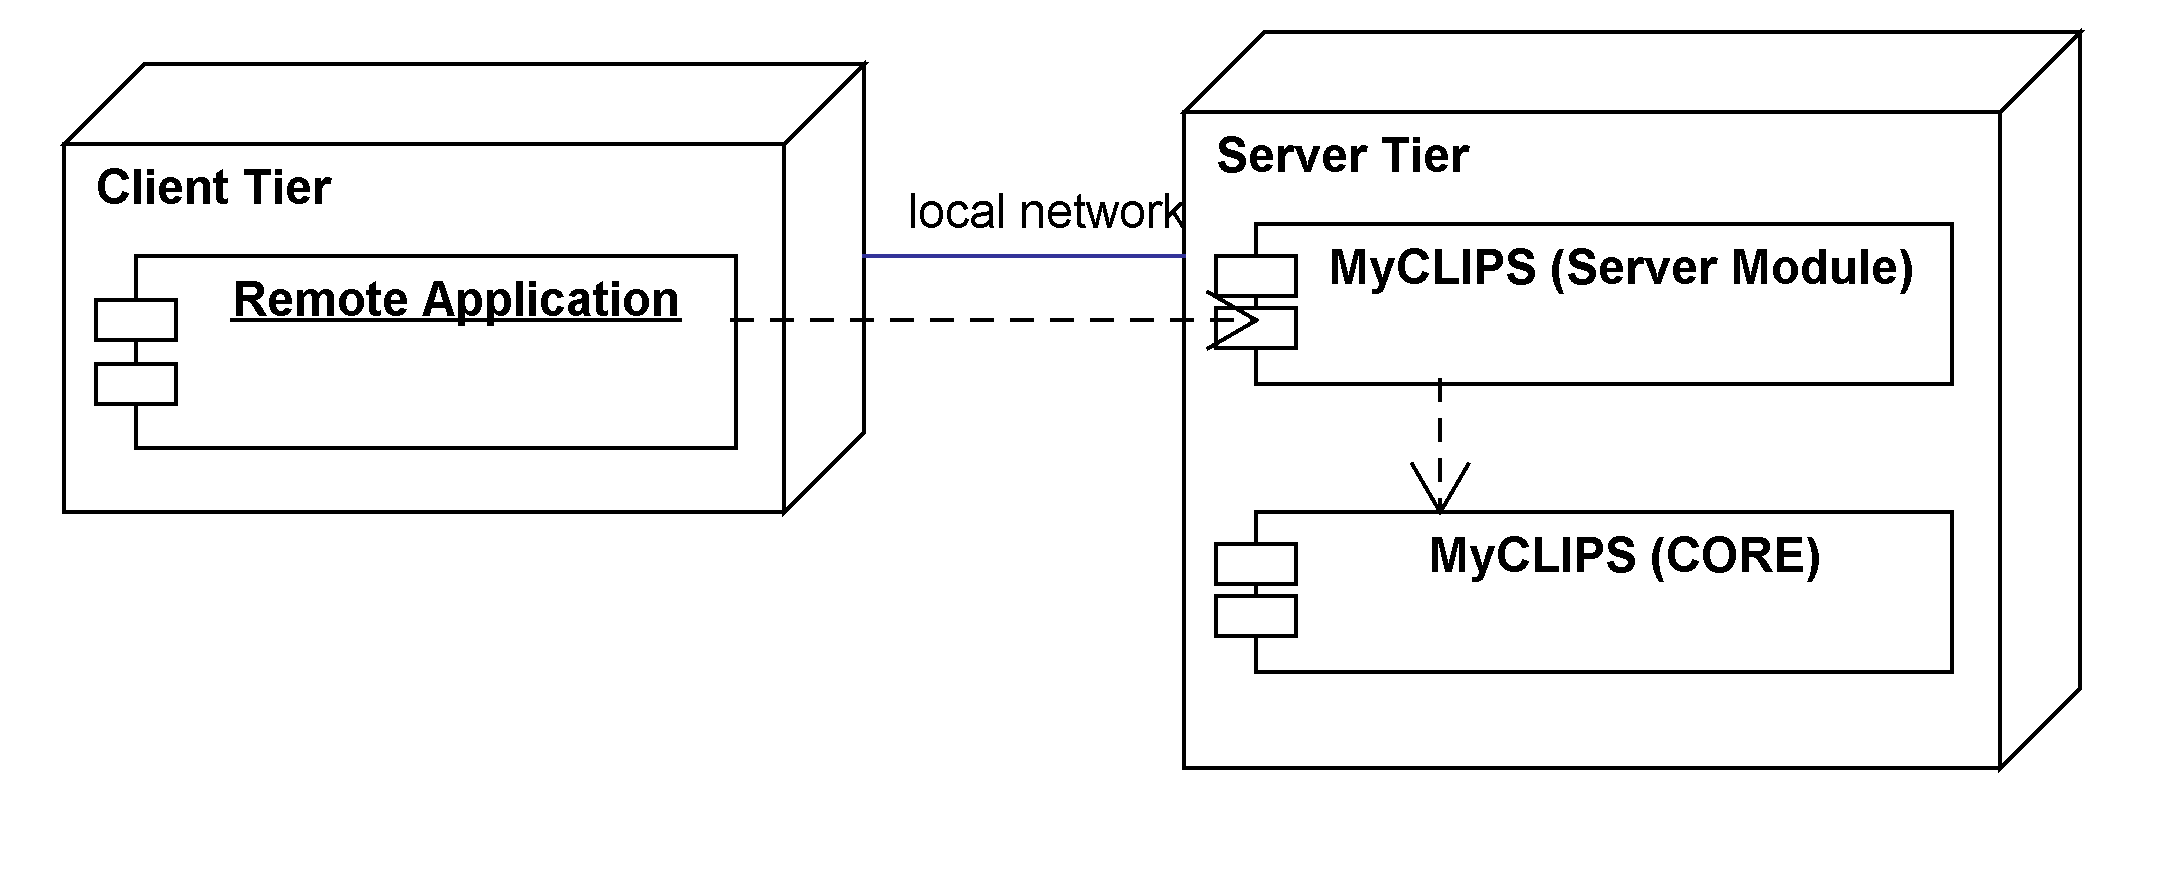
\includegraphics[width=0.8\textwidth]{Immagini/Capitolo3/Deployment/Client-Server.png}
\caption[Vista generale dell'architettura di sistema]{Vista generale dell'architettura di sistema: i servizi offerti dal modulo principale vengono distribuiti ad una serie di applicazioni remote attraverso l'utilizzo del componente Server}\label{fig:architettura-client-server}
\end{figure}

Il sistema è composto da due componenti principali distinte. Una prima, il \emph{core} del sistema MyCLIPS, realizza i servizi previsti dall'environment in una serie di API. Una seconda, il \emph{modulo server}, si pone come tramite fra i servizi offerti dalla prima componente e un gruppo di client, distribuendo le caratteristiche attraverso un modello d'architettura \emph{Client-Server}~(\figurename~\ref{fig:architettura-client-server}).

\begin{figure}[h]
\centering
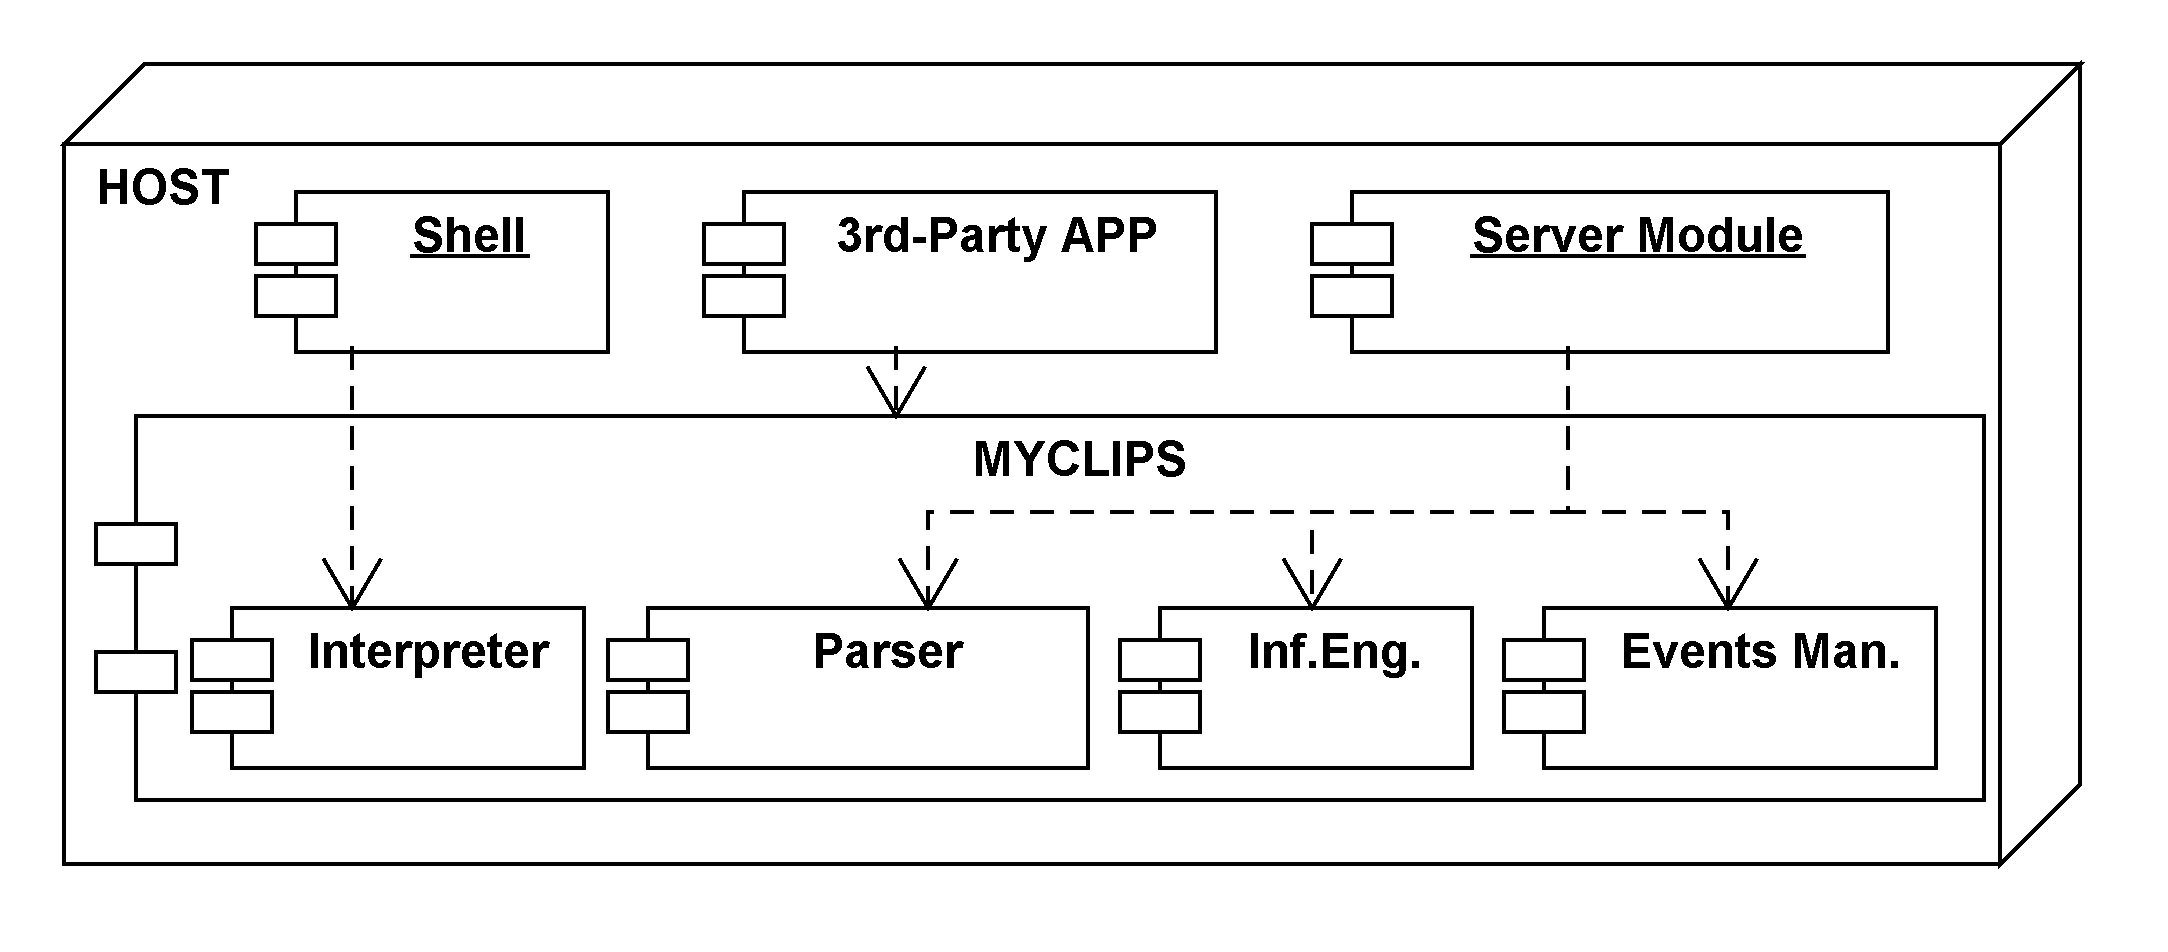
\includegraphics[width=0.9\textwidth]{Immagini/Capitolo3/Deployment/Shell-3rdPartyApp.png}
\caption[Vista generale dell'architettura locale di sistema]{Vista generale dell'architettura locale di sistema: i componenti del \emph{core} vengono utilizzati da componenti esterne (\emph{shell}, \emph{modulo server} o applicazioni generiche)}\label{fig:architettura-3rdparty}
\end{figure}

Il \emph{modulo server} è sia un elemento di sistema che un esempio d'istanza di applicazione generica che utilizza i servizi offerti dal \emph{core}. Un altro esempio è quello del componente \emph{shell}: un elemento distinto che utilizza le interfacce del \emph{core} per realizzare un terminale testuale con il quale utilizzare l'\emph{environment}~(\figurename~\ref{fig:architettura-3rdparty}).


\subsection{Core}

La componente principale è quella rappresentata dal \emph{core} di MyCLIPS: racchiude tutti i \emph{package} necessari alla realizzazione dei servizi principali del sistema~(\figurename~\ref{fig:packages-myclips}).

\begin{figure}[h]
\centering
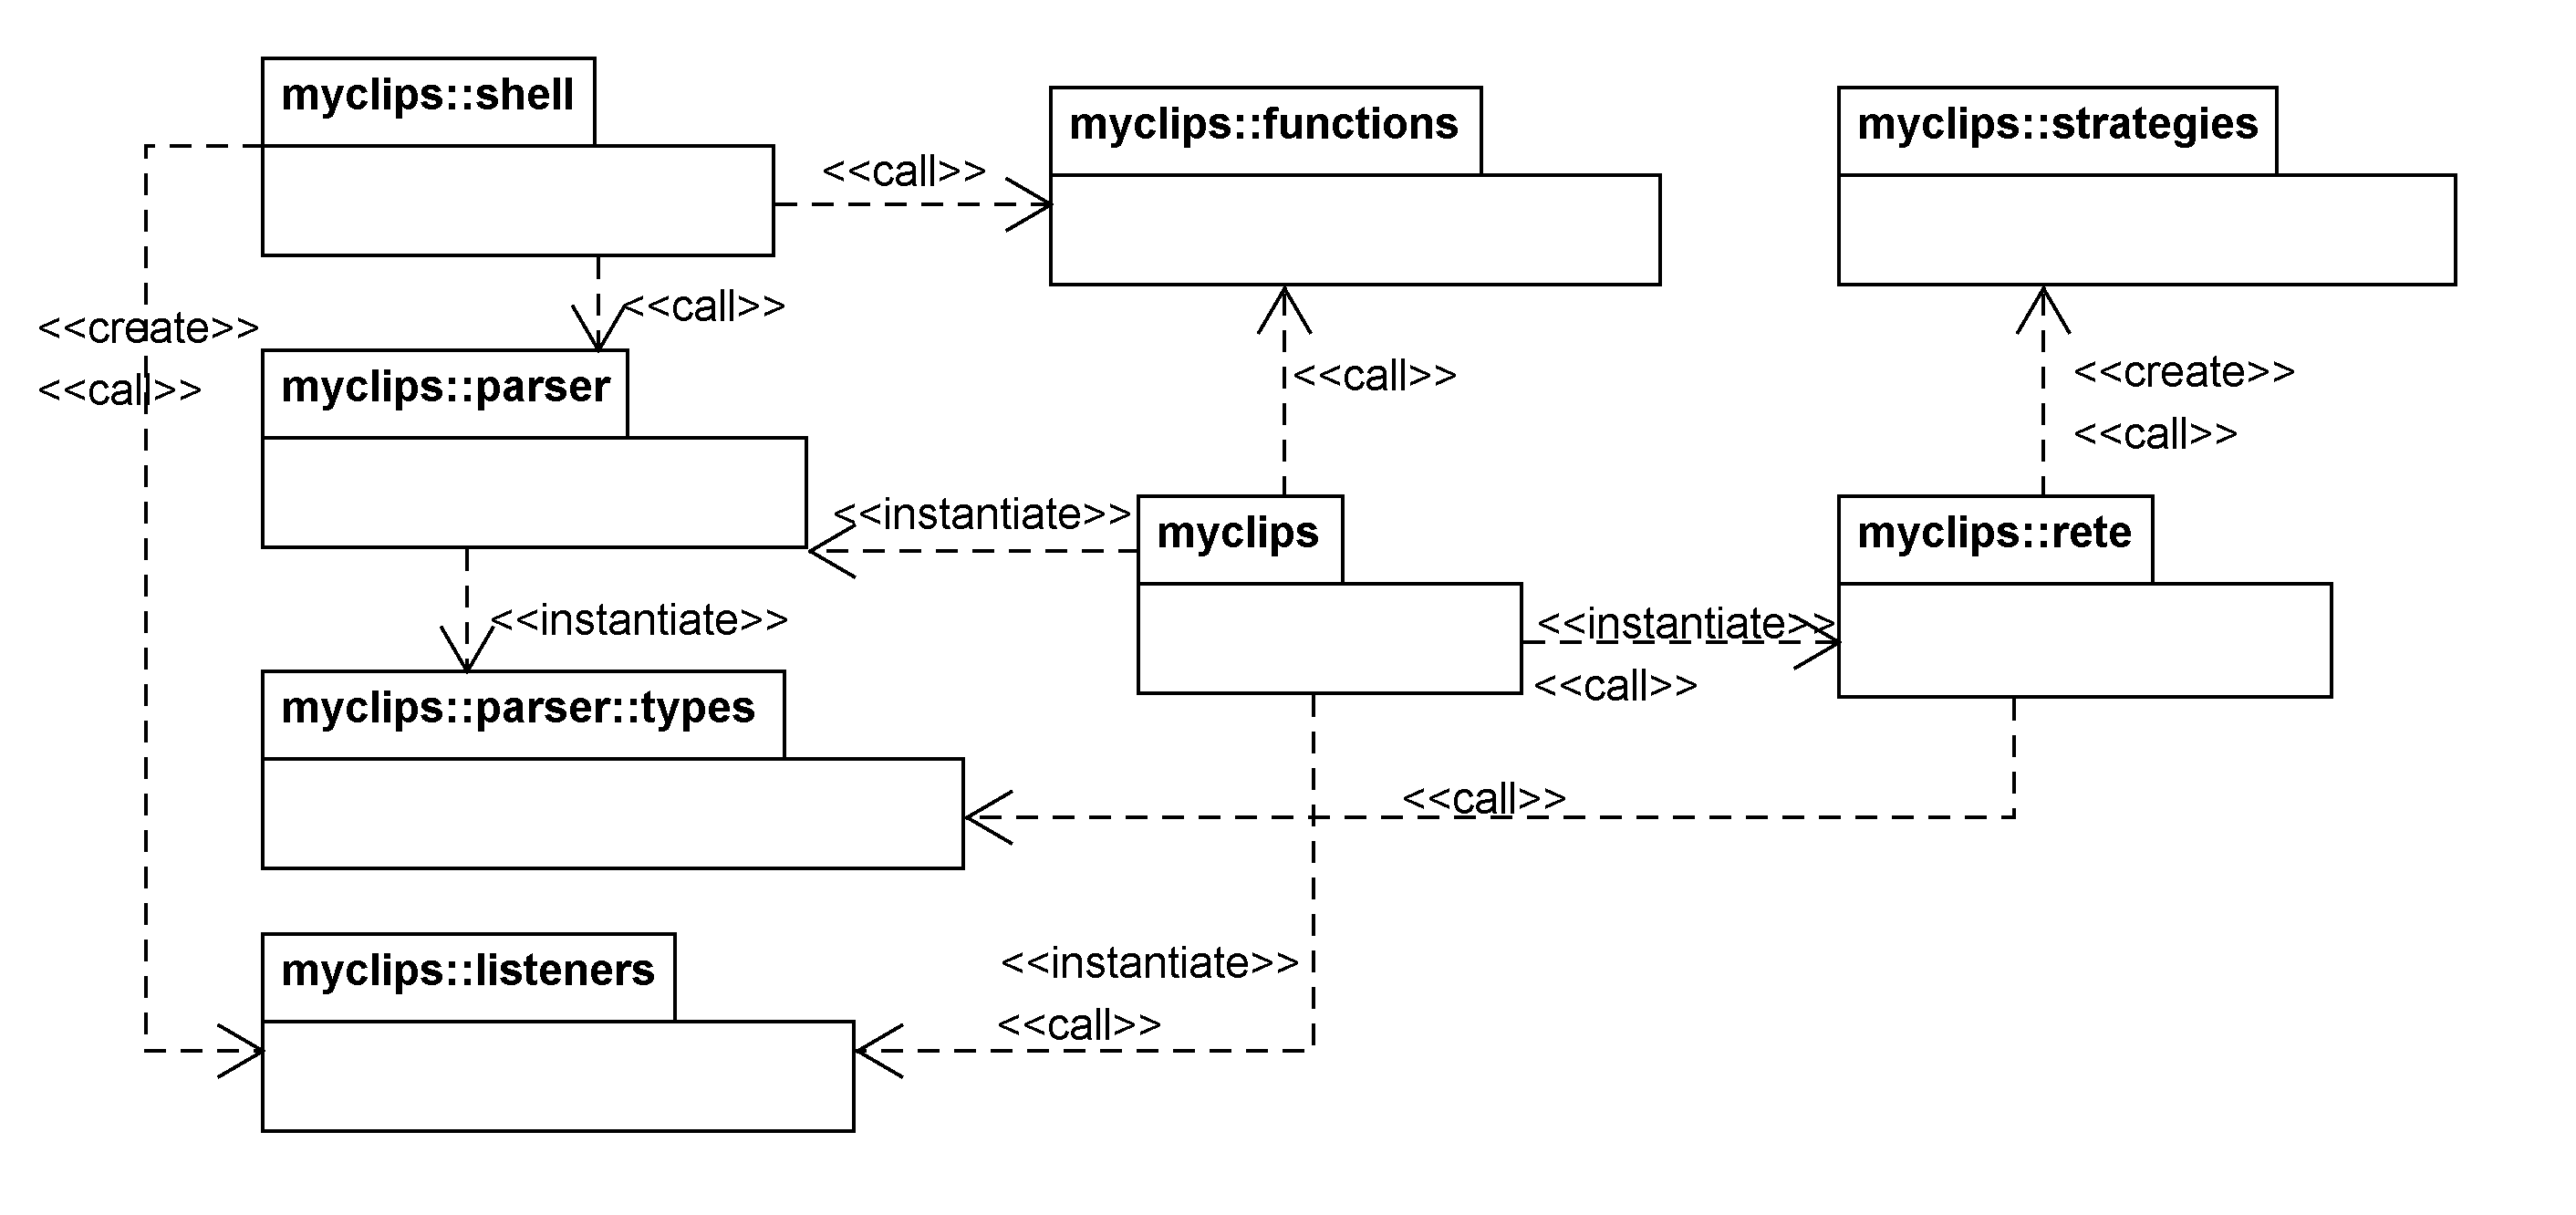
\includegraphics[width=1\textwidth]{Immagini/Capitolo3/Packages/Core.png}
\caption{Package \emph{myclips}: vista dei \emph{package} che compongono il \emph{core}}\label{fig:packages-myclips}
\end{figure}

%Lo scopo dei singoli \emph{package}, con riferimento alle funzionalità che realizzano, è dettagliato nel proseguo dei paragrafi.

\subsubsection{Modulo Parser}

\begin{figure}[h]
\centering
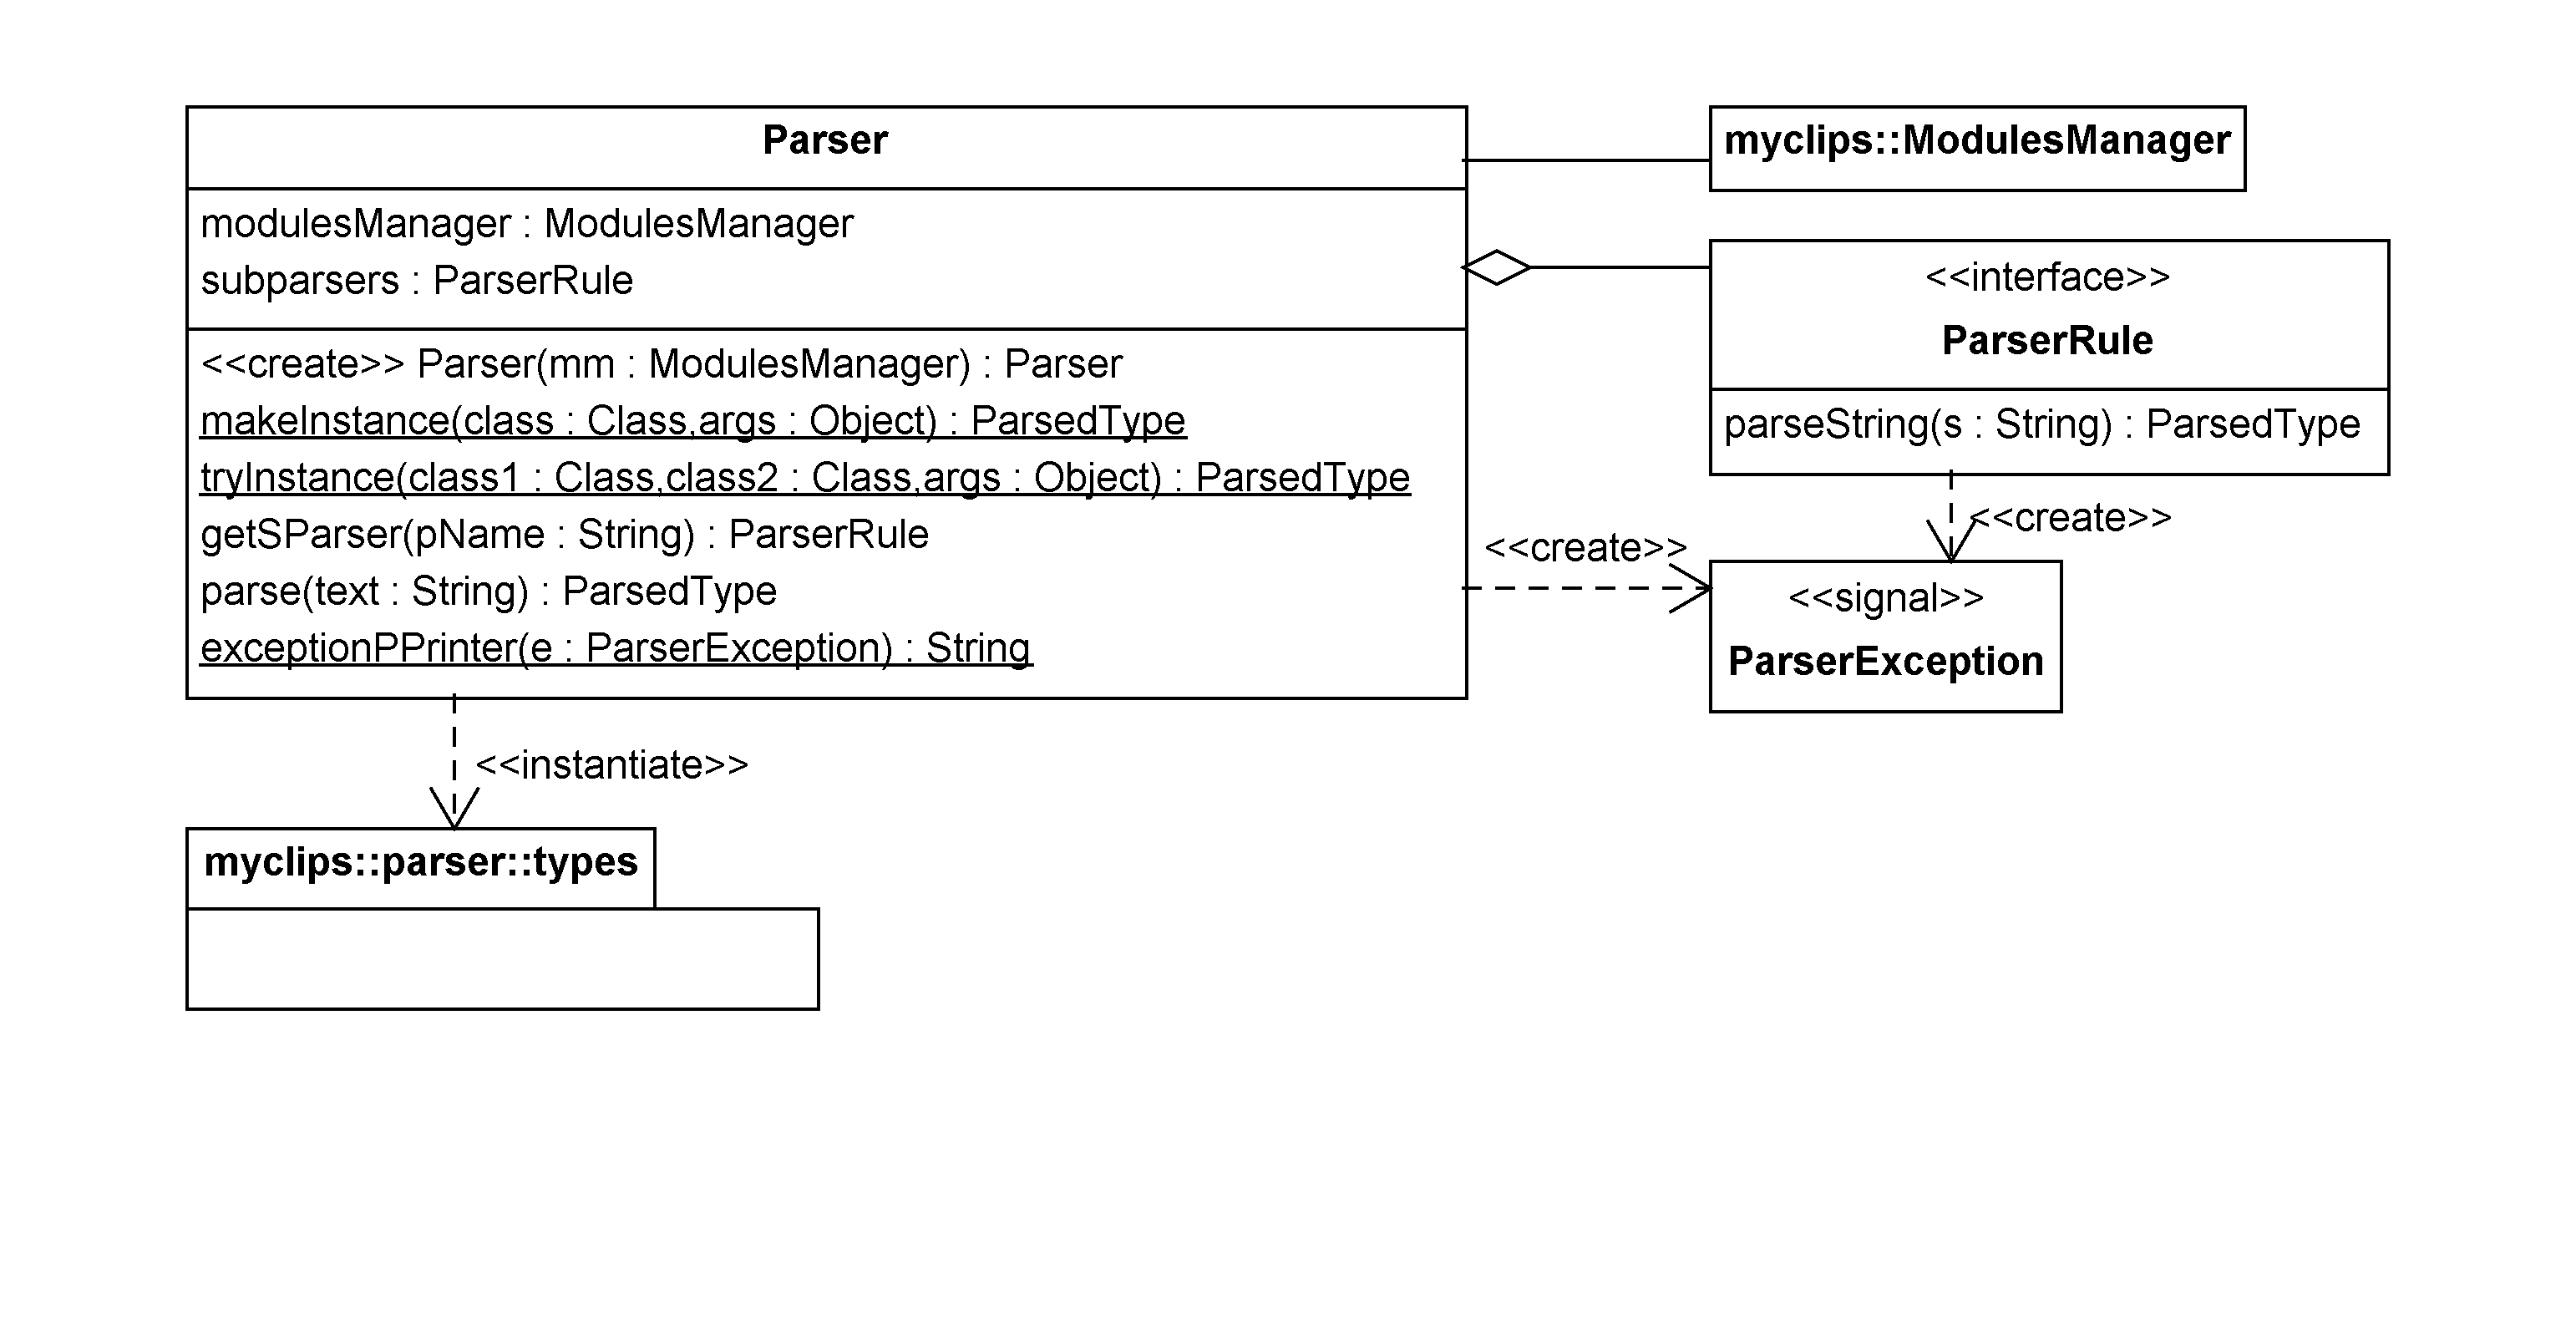
\includegraphics[width=1\textwidth]{Immagini/Capitolo3/Classi/myclips_parser_Parser.png}
\caption{Package \emph{myclips.parser}: vista delle classi relative al \emph{Parser}}\label{fig:class-myclips-parser-Parser}
\end{figure}

Il \emph{package} \emph{Parser} comprende l'insieme di classi e interfacce che realizzano la funzionalità di analisi e conversione del linguaggio di specifica in istanze utilizzabili dal motore inferenziale per il compimento delle proprie attività.

L'elemento principale del \emph{package} è la classe \emph{Parser}~(\figurename~\ref{fig:class-myclips-parser-Parser}), che organizza le regole di conversione (rappresentate dall'interfaccia \emph{ParserRule}) ed effettua le operazioni di conversione del testo in istanze. Le classi utilizzate per la rappresentazione dei costrutti convertiti sono organizzate all'interno del \emph{sub-package} \emph{myclips.parser.types}.

Il \emph{sub-package} contiene l'insieme di classi relative alla rappresentazione dei tipi atomici di base e dei costrutti compositi.

\begin{figure}[h]
\centering
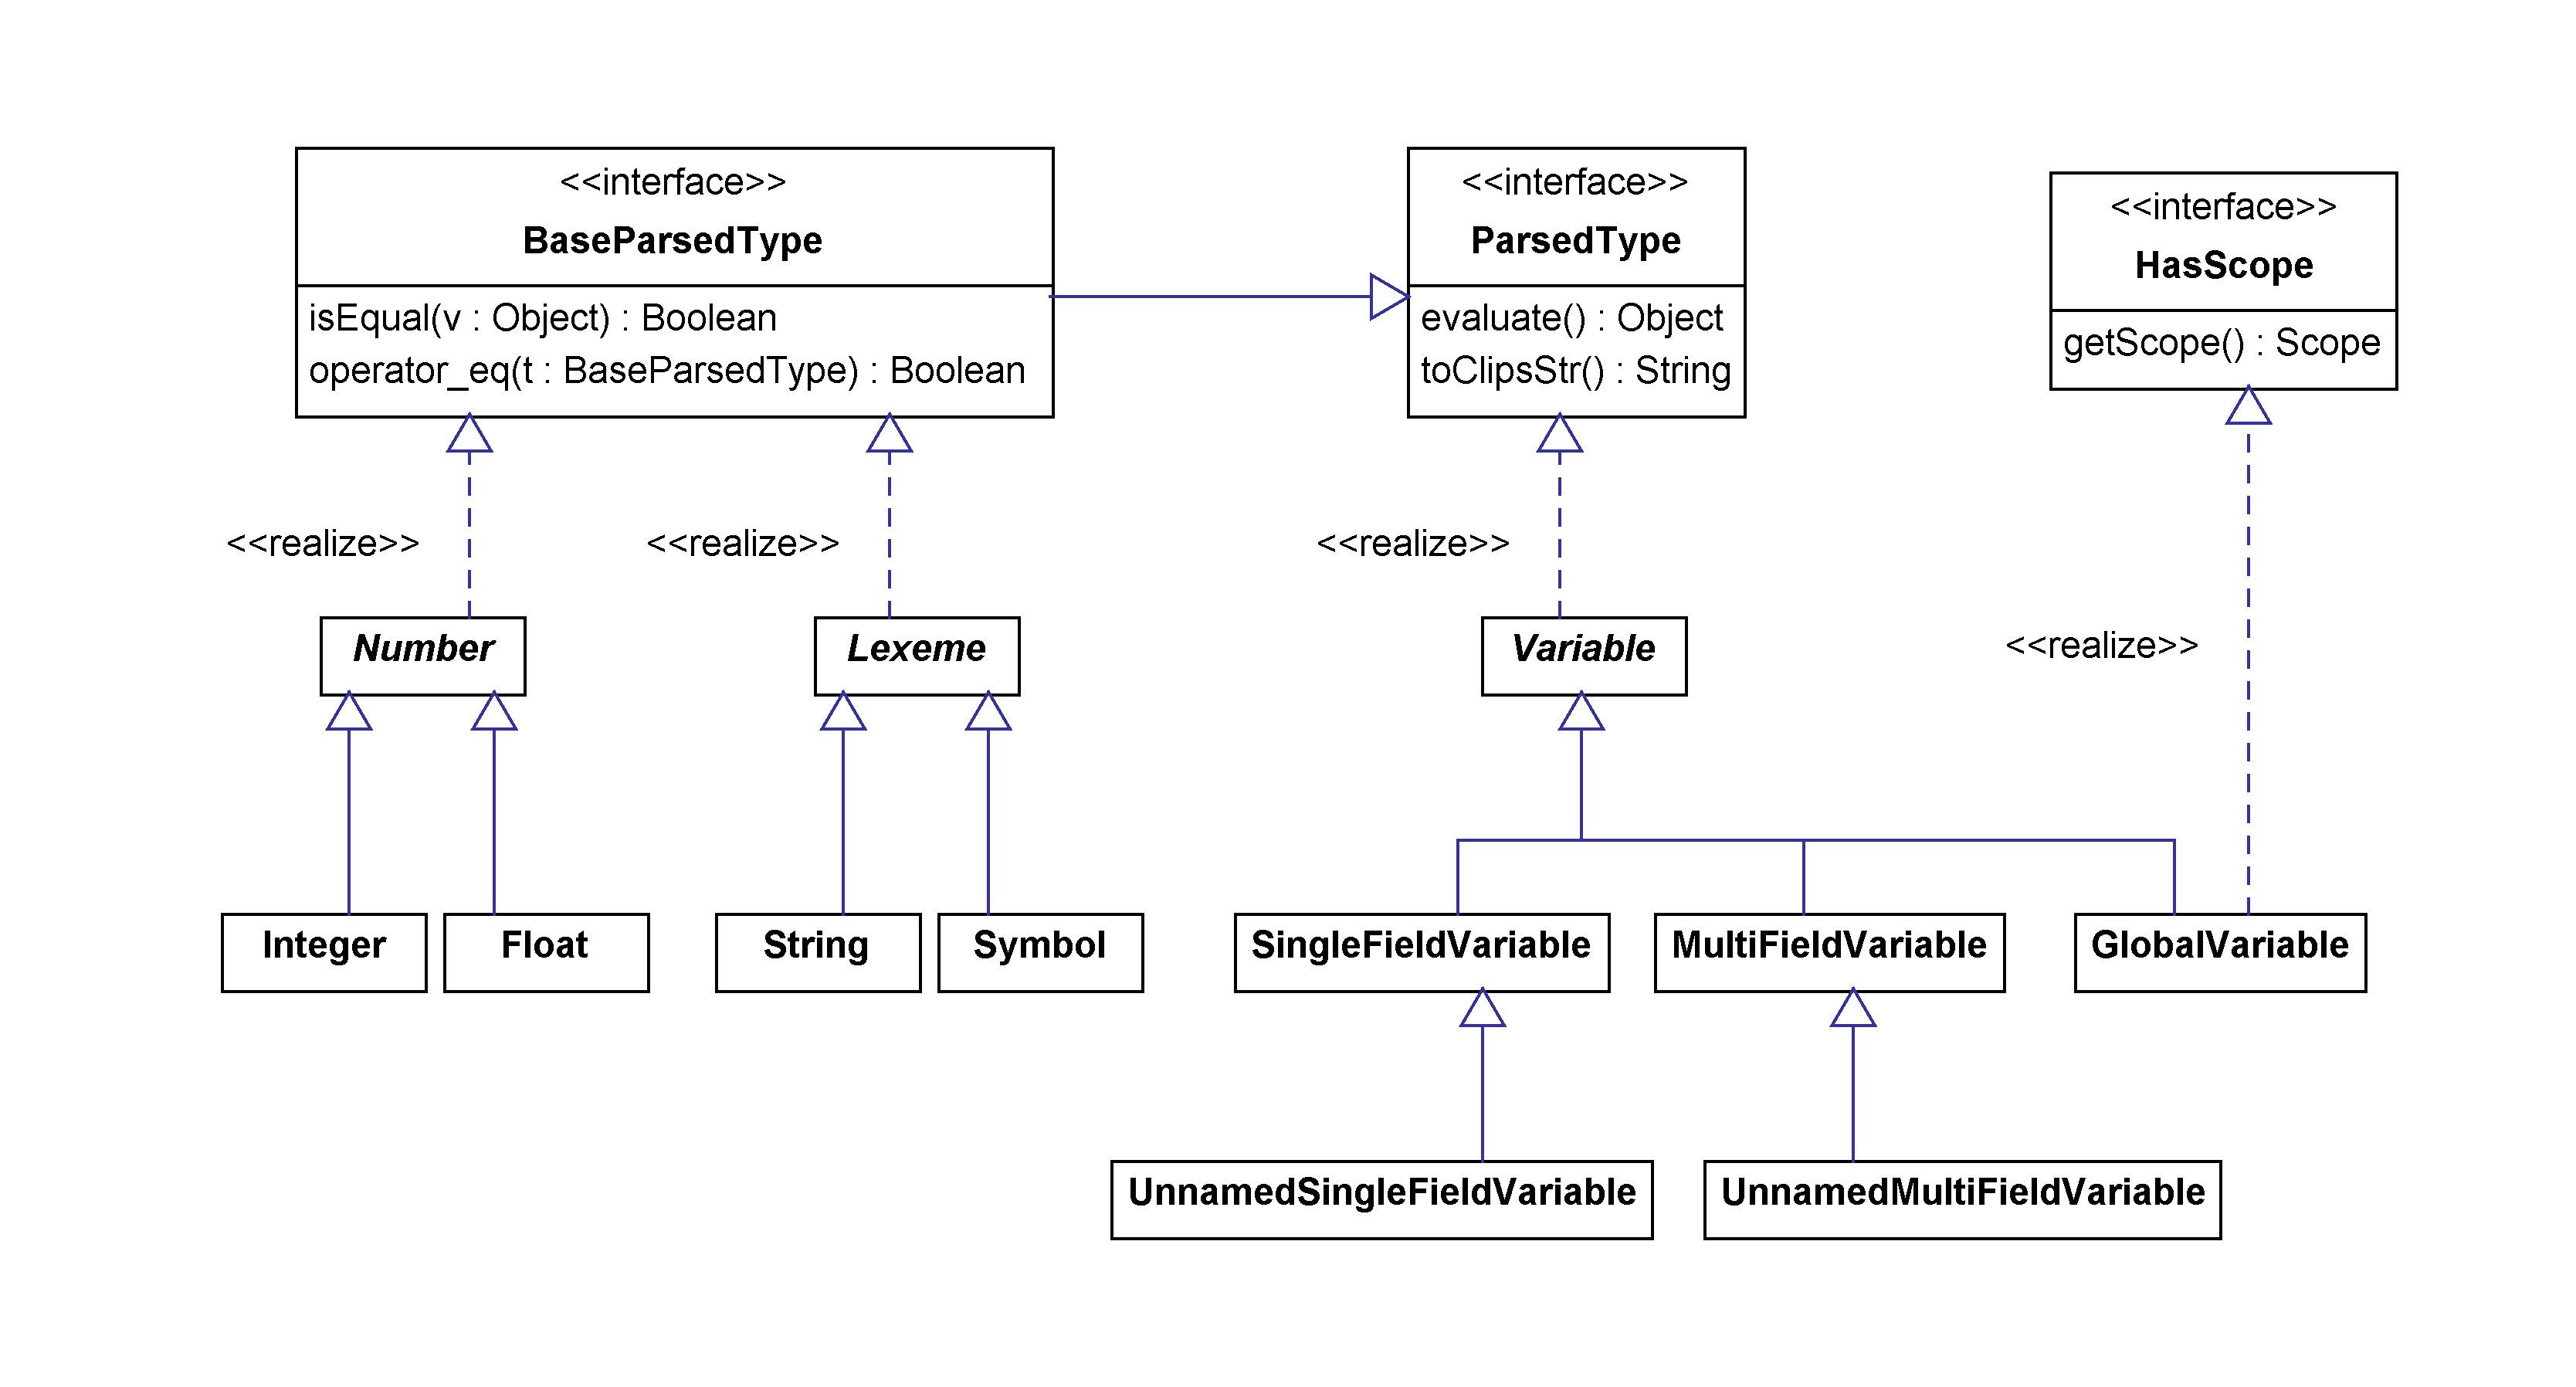
\includegraphics[width=0.8\textwidth]{Immagini/Capitolo3/Classi/myclips_parser_types_Atoms.png}
\caption{Package \emph{myclips.parser.types}: vista di classi e interfacce per gli elementi atomici}\label{fig:class-myclips-parser-types-Atoms}
\end{figure}

La gerarchia di tipi atomici supportata dal sistema segue le specifiche relative ai tipi proposti da CLIPS. Fanno parte di questa classificazione \emph{Lexeme}, specializzato da \emph{Symbol} e \emph{String}, e \emph{Number}, specializzato da \emph{Integer} e \emph{Float}. A questi tipi si uniscono quelli per la rappresentazioni delle variabili~(\figurename~\ref{fig:class-myclips-parser-types-Atoms}).

\begin{figure}[h]
\centering
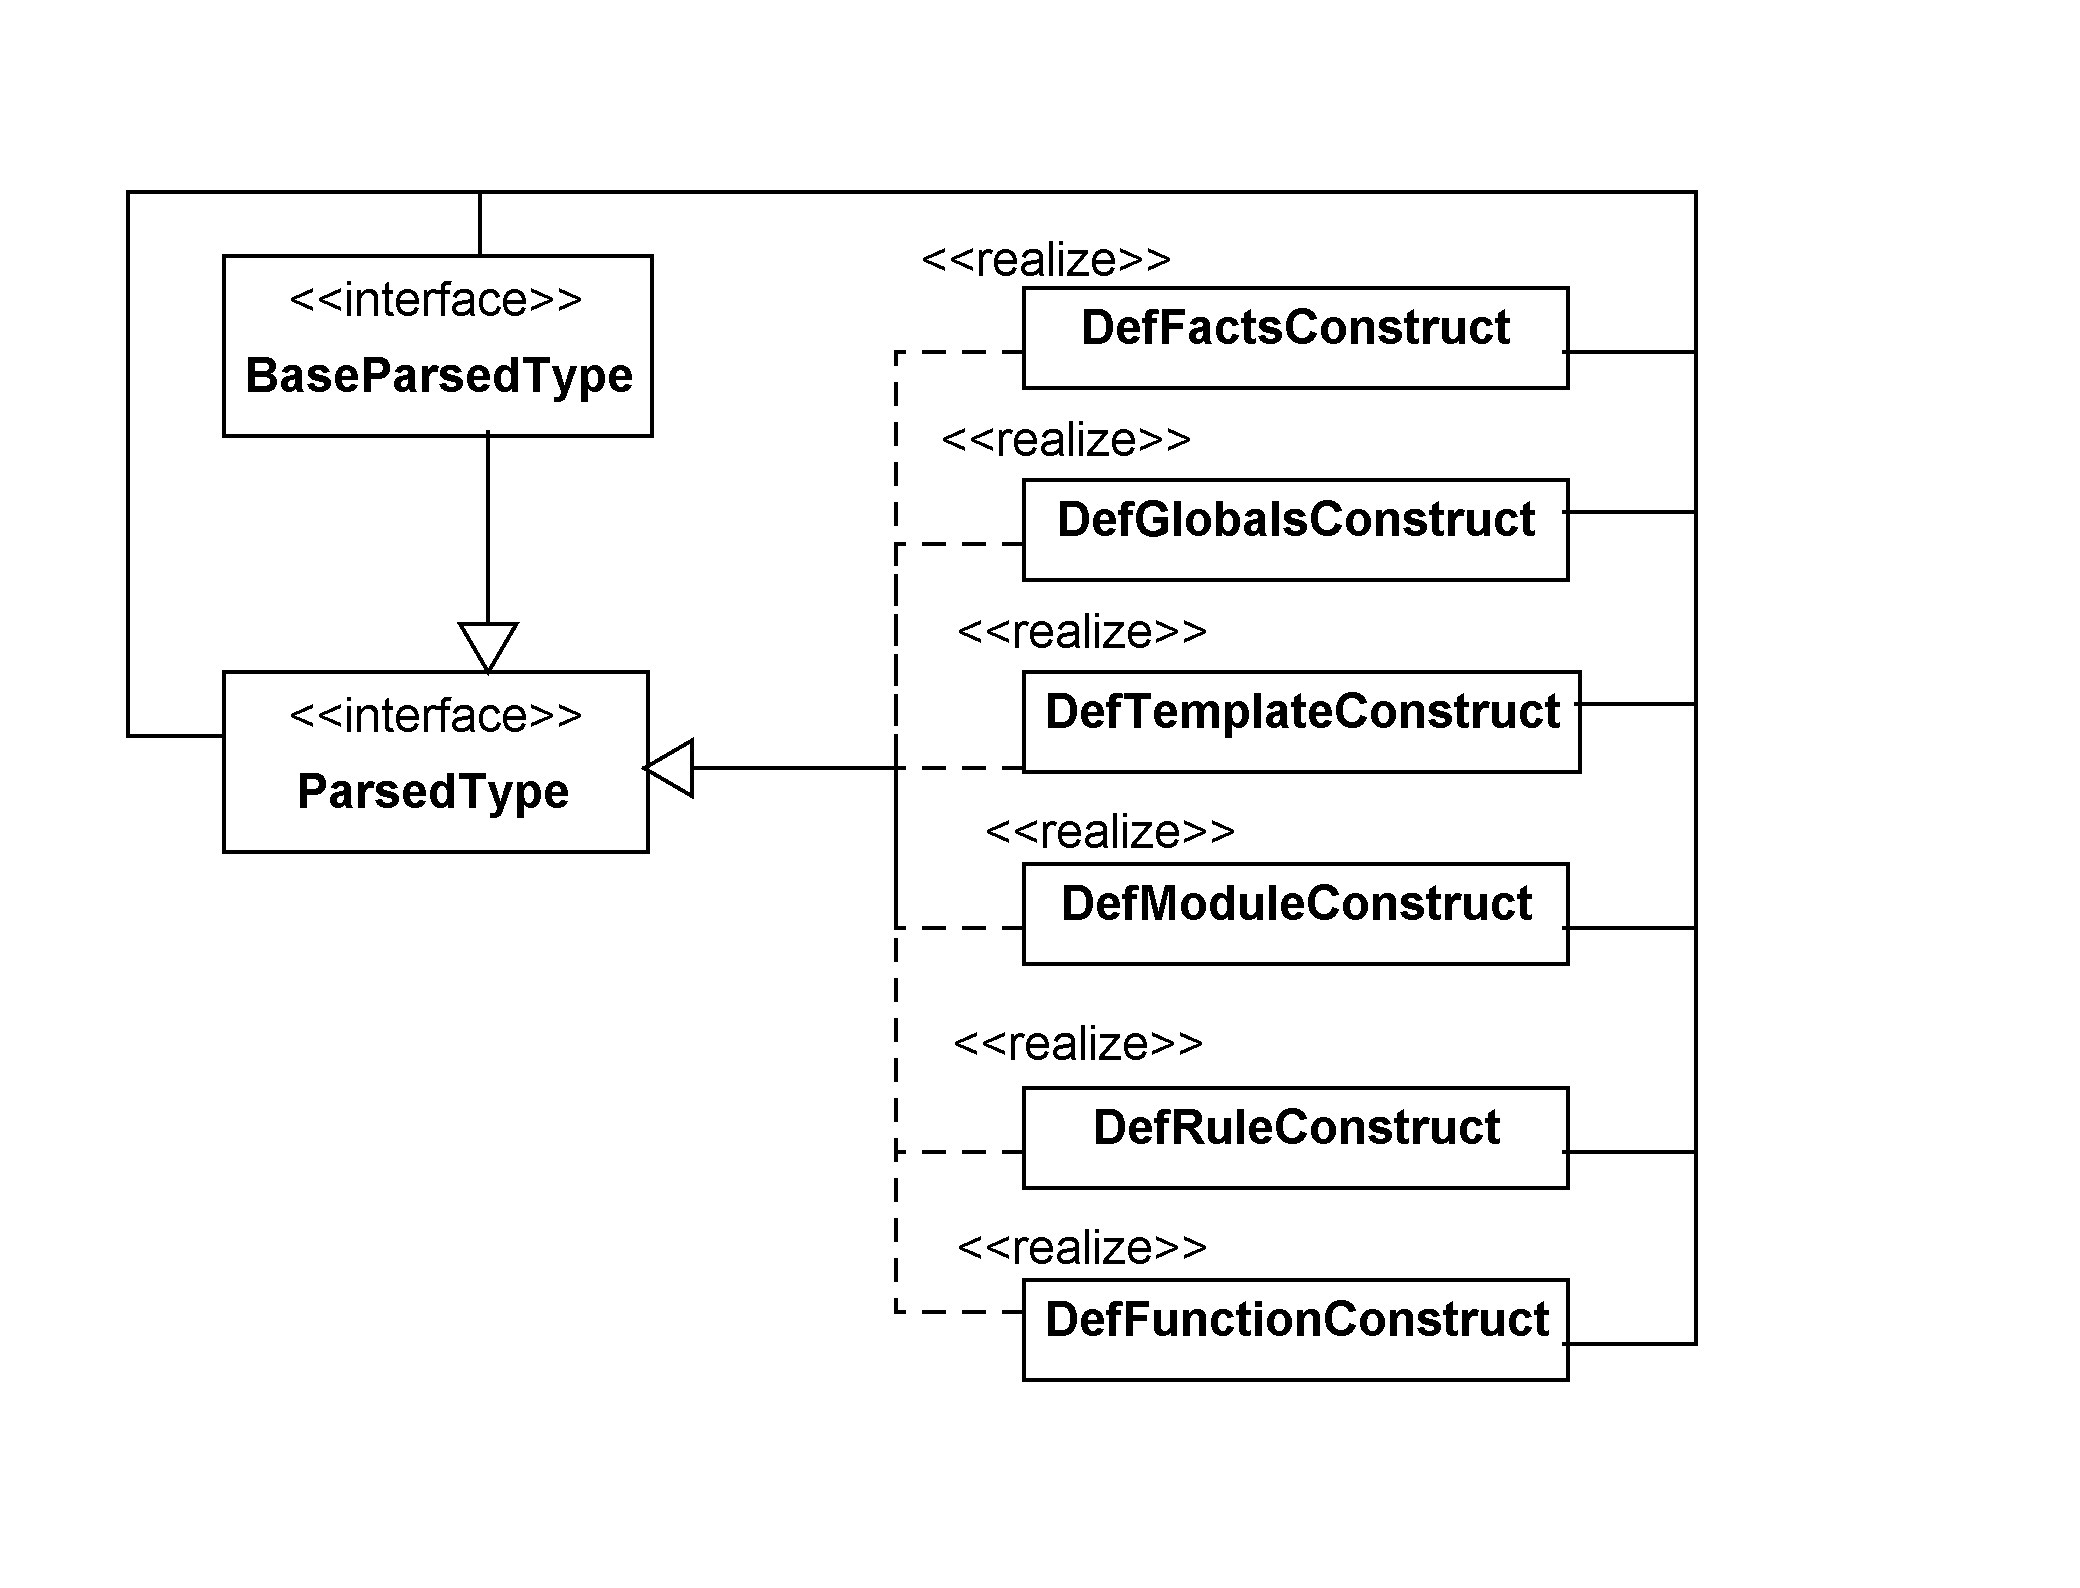
\includegraphics[width=0.8\textwidth]{Immagini/Capitolo3/Classi/myclips_parser_types_Constructs.png}
\caption{Package \emph{myclips.parser.types}: vista di classi e interfacce per i costrutti principali}\label{fig:class-myclips-parser-types-Constructs}
\end{figure}

La composizione dei tipi di base realizza un insieme di costrutti complessi principali. Le classi mostrate in \figurename~\ref{fig:class-myclips-parser-types-Constructs} sono le rappresentazioni corrispondenti ai formalismi \emph{defrule}, \emph{defglobals}, \emph{deffunction}, \emph{deftemplate} e \emph{defmodule}, utilizzate dal linguaggio di specifica per la formalizzazione dei sistemi esperti.

\begin{figure}[h]
\centering
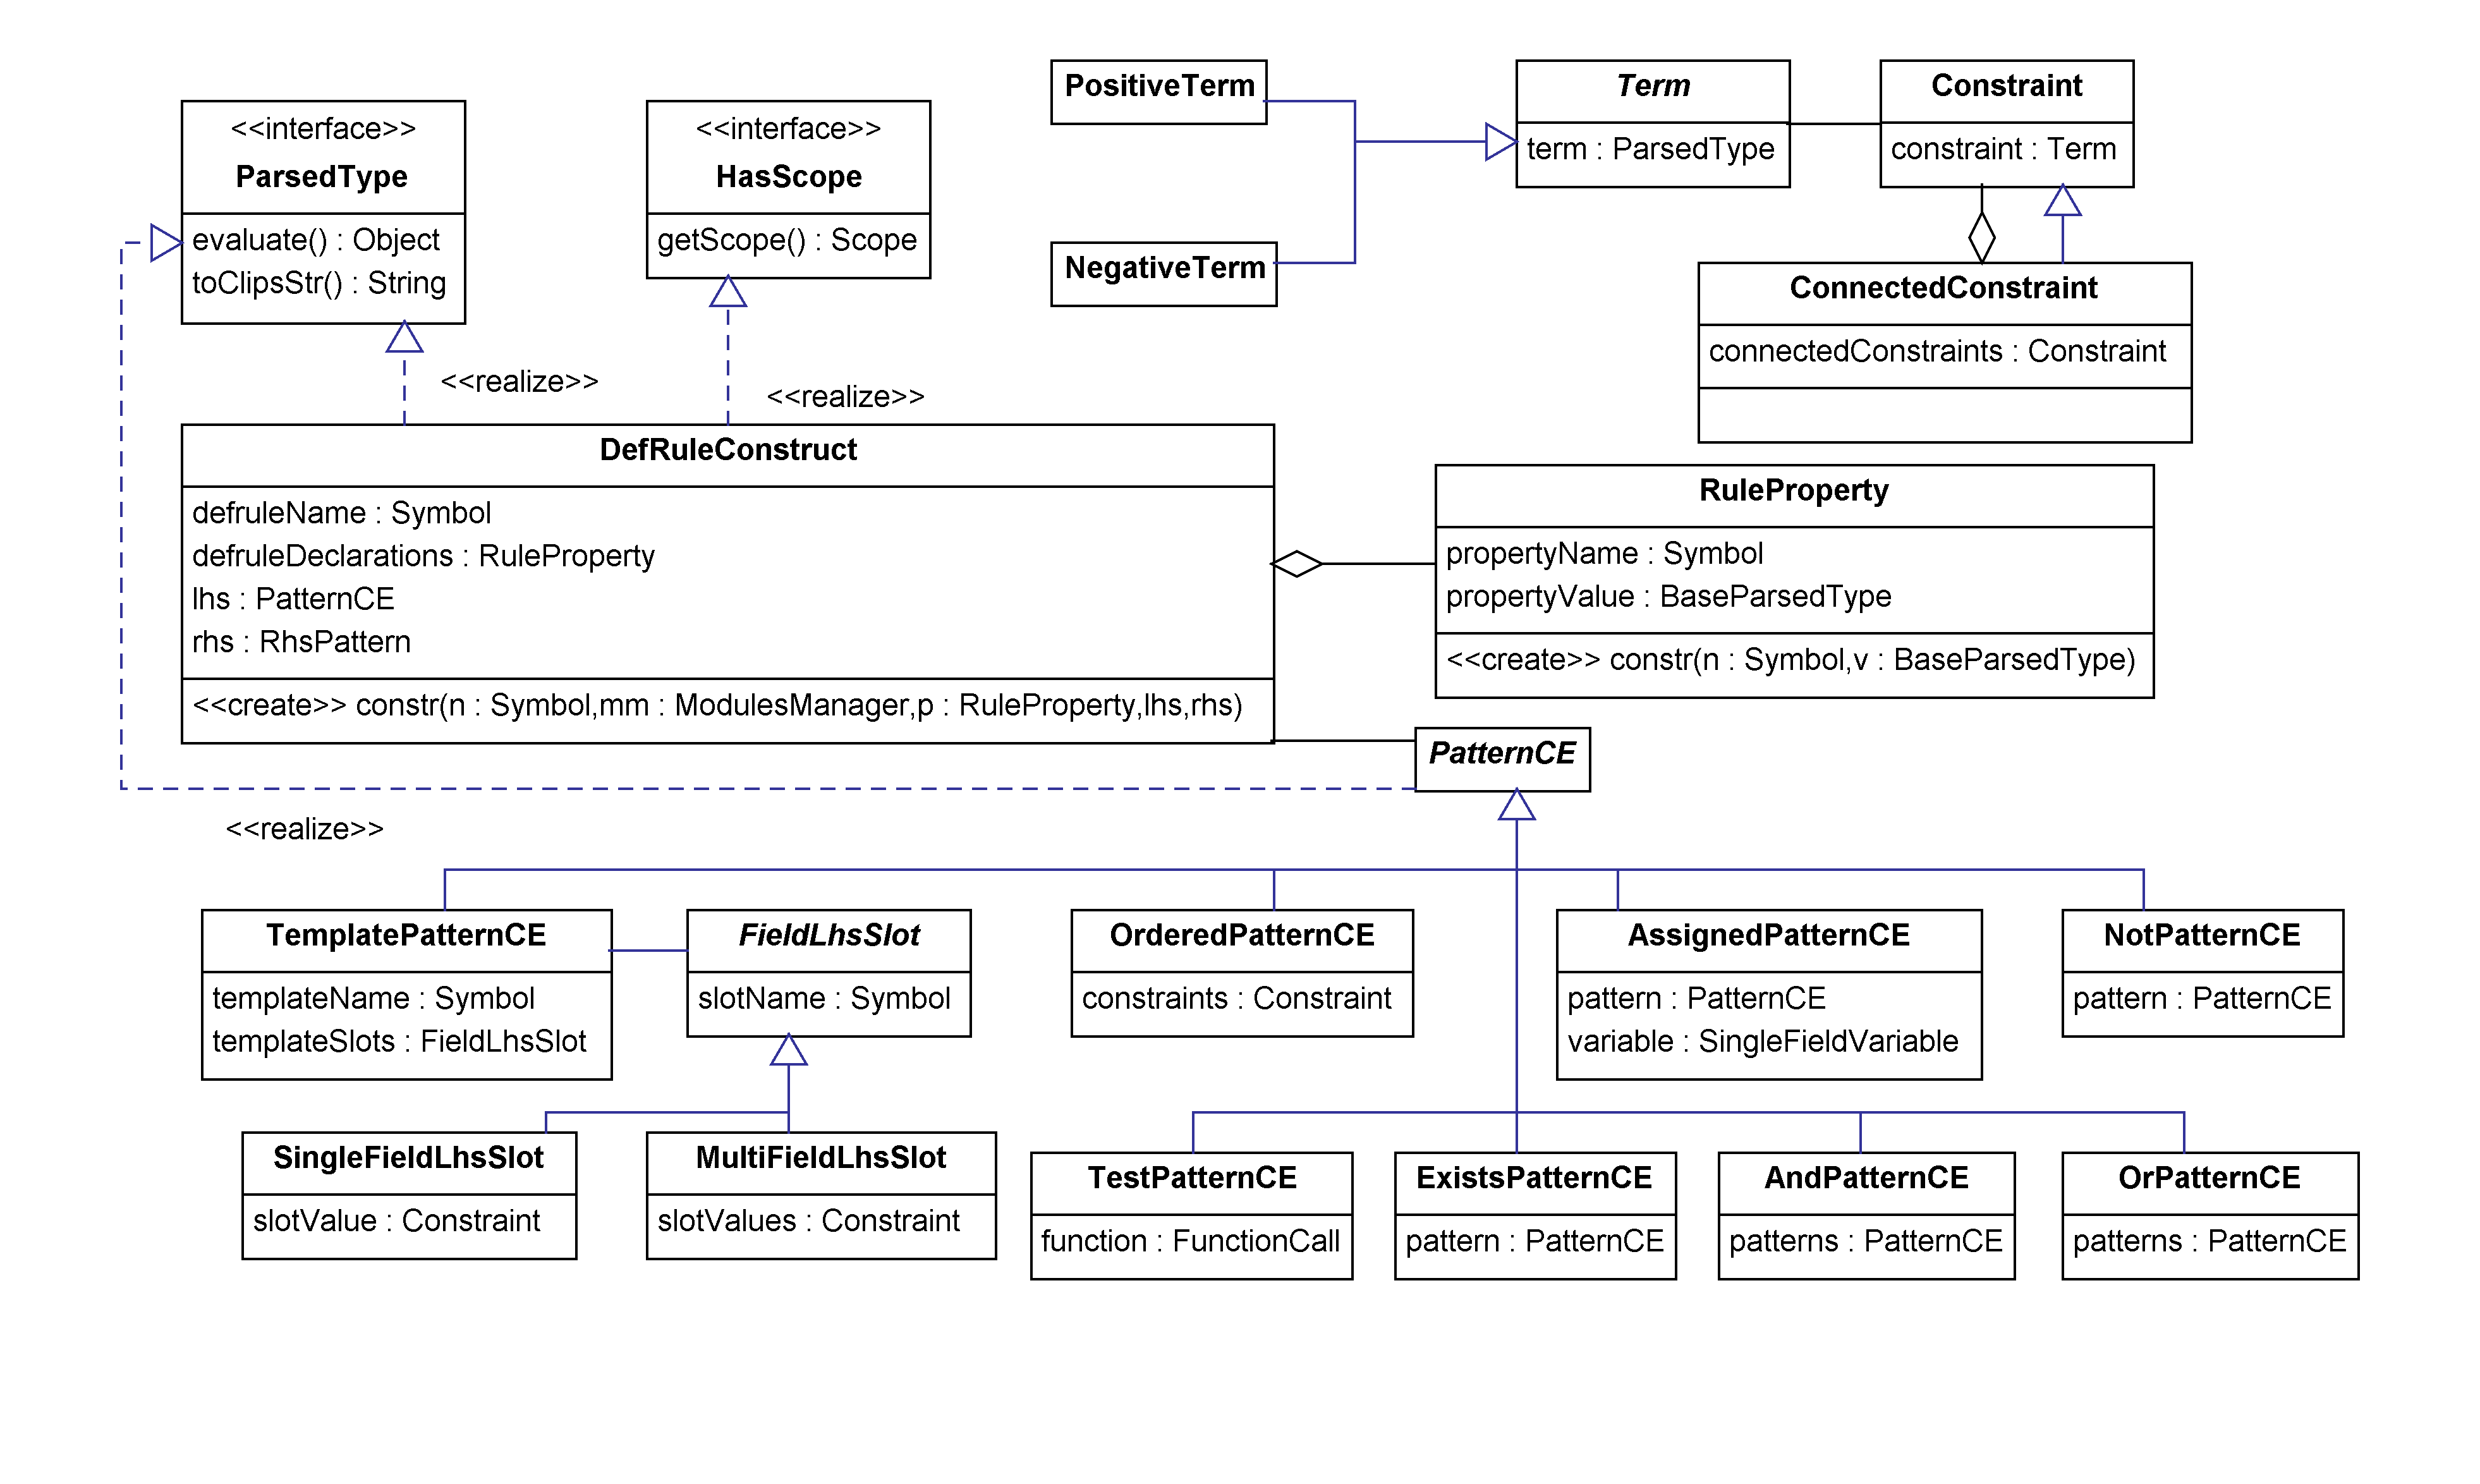
\includegraphics[width=1\textwidth]{Immagini/Capitolo3/Classi/myclips_parser_types_DefRule.png}
\caption{Package \emph{myclips.parser.types}: vista delle classi e interfacce relative al costrutto \emph{defrule}}\label{fig:class-myclips-parser-types-DefRuleConstruct}
\end{figure}

%\begin{figure}[h]
%\centering
%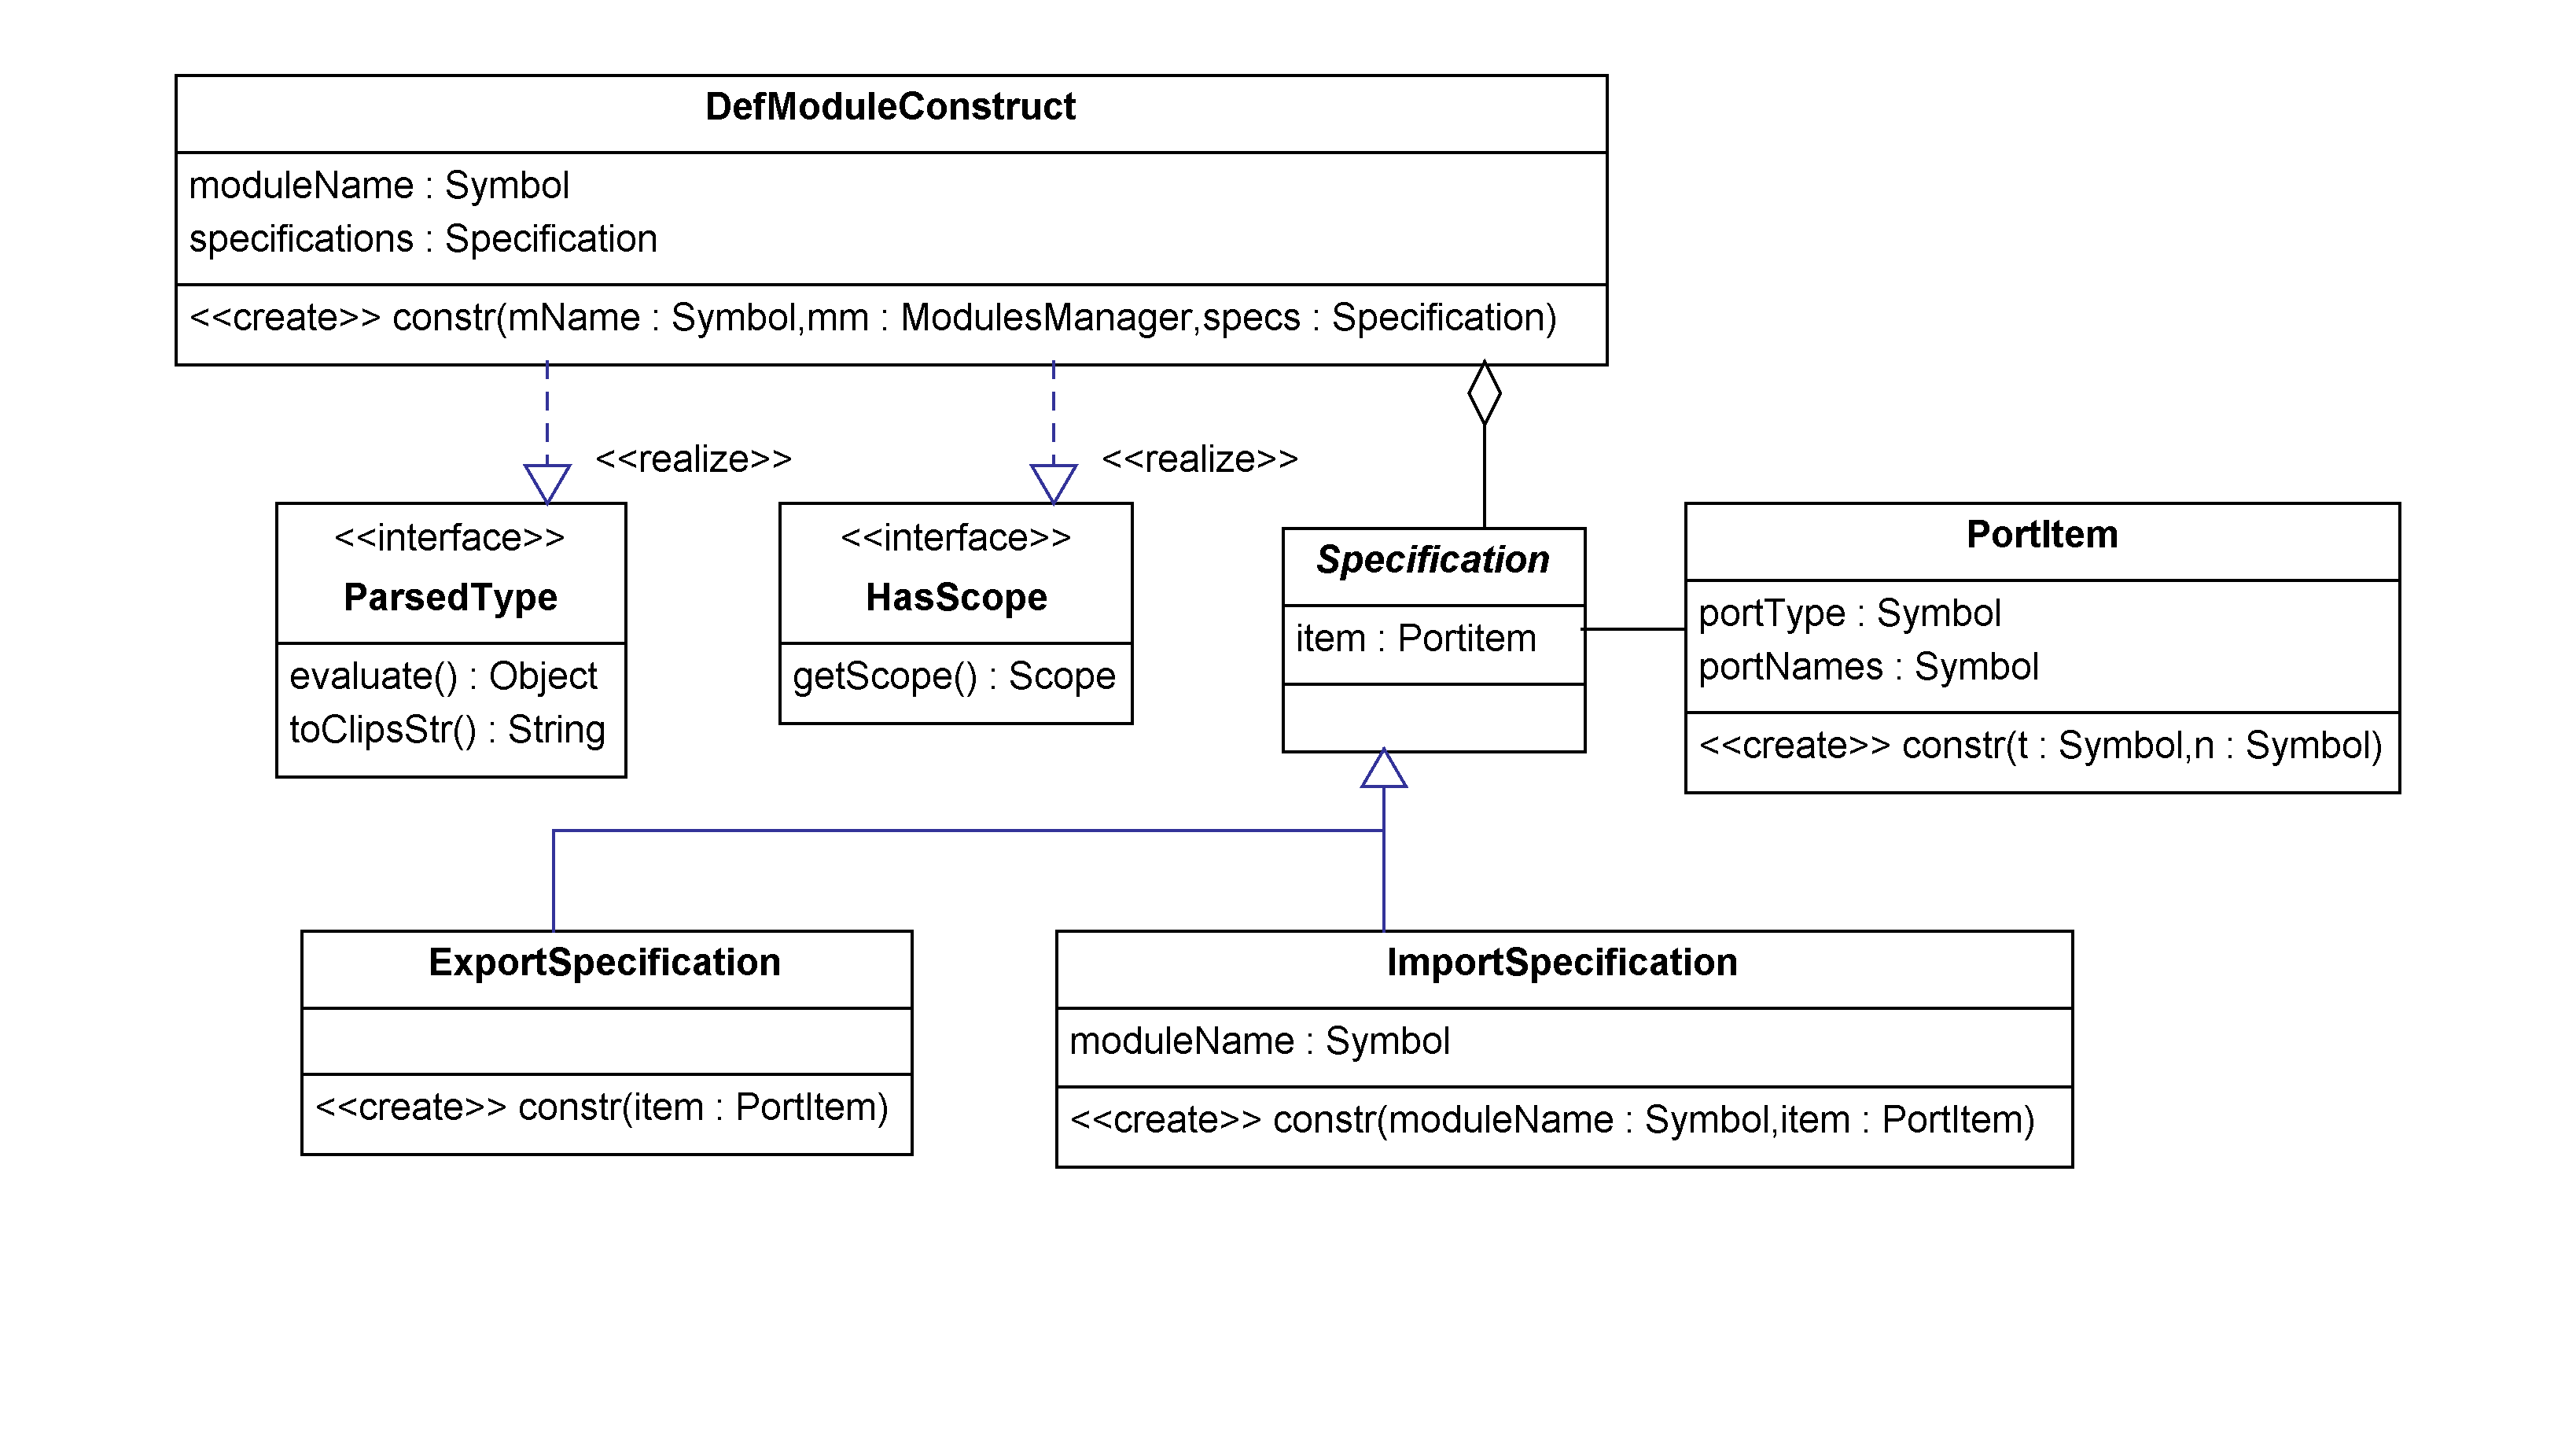
\includegraphics[width=0.9\textwidth]{Immagini/Capitolo3/Classi/myclips_parser_types_DefModule.png}
%\caption{Package \emph{myclips.parser.types}: vista delle classi e interfacce relative al costrutto \emph{defmodule}}\label{fig:class-myclips-parser-types-DefModuleConstruct}
%\end{figure}


%A titolo d'esempio di propongono le strutture delle classi \emph{DefRuleConstruct}~(\figurename~\ref{fig:class-myclips-parser-types-DefRuleConstruct}) e \emph{DefModuleConstruct}~(\figurename~\ref{fig:class-myclips-parser-types-DefModuleConstruct}), insieme ad i relativi sotto-costrutti utilizzati per la conversione e rappresentazione di pozioni di quest'ultimi.

A titolo d'esempio si propone la struttura della classe \emph{DefRuleConstruct}~(\figurename~\ref{fig:class-myclips-parser-types-DefRuleConstruct})  insieme ad i relativi sotto-costrutti utilizzati per la conversione e rappresentazione di pozioni di quest'ultima.

\clearpage

\subsubsection{Modulo Motore Inferenziale}

\begin{figure}[h]
\centering
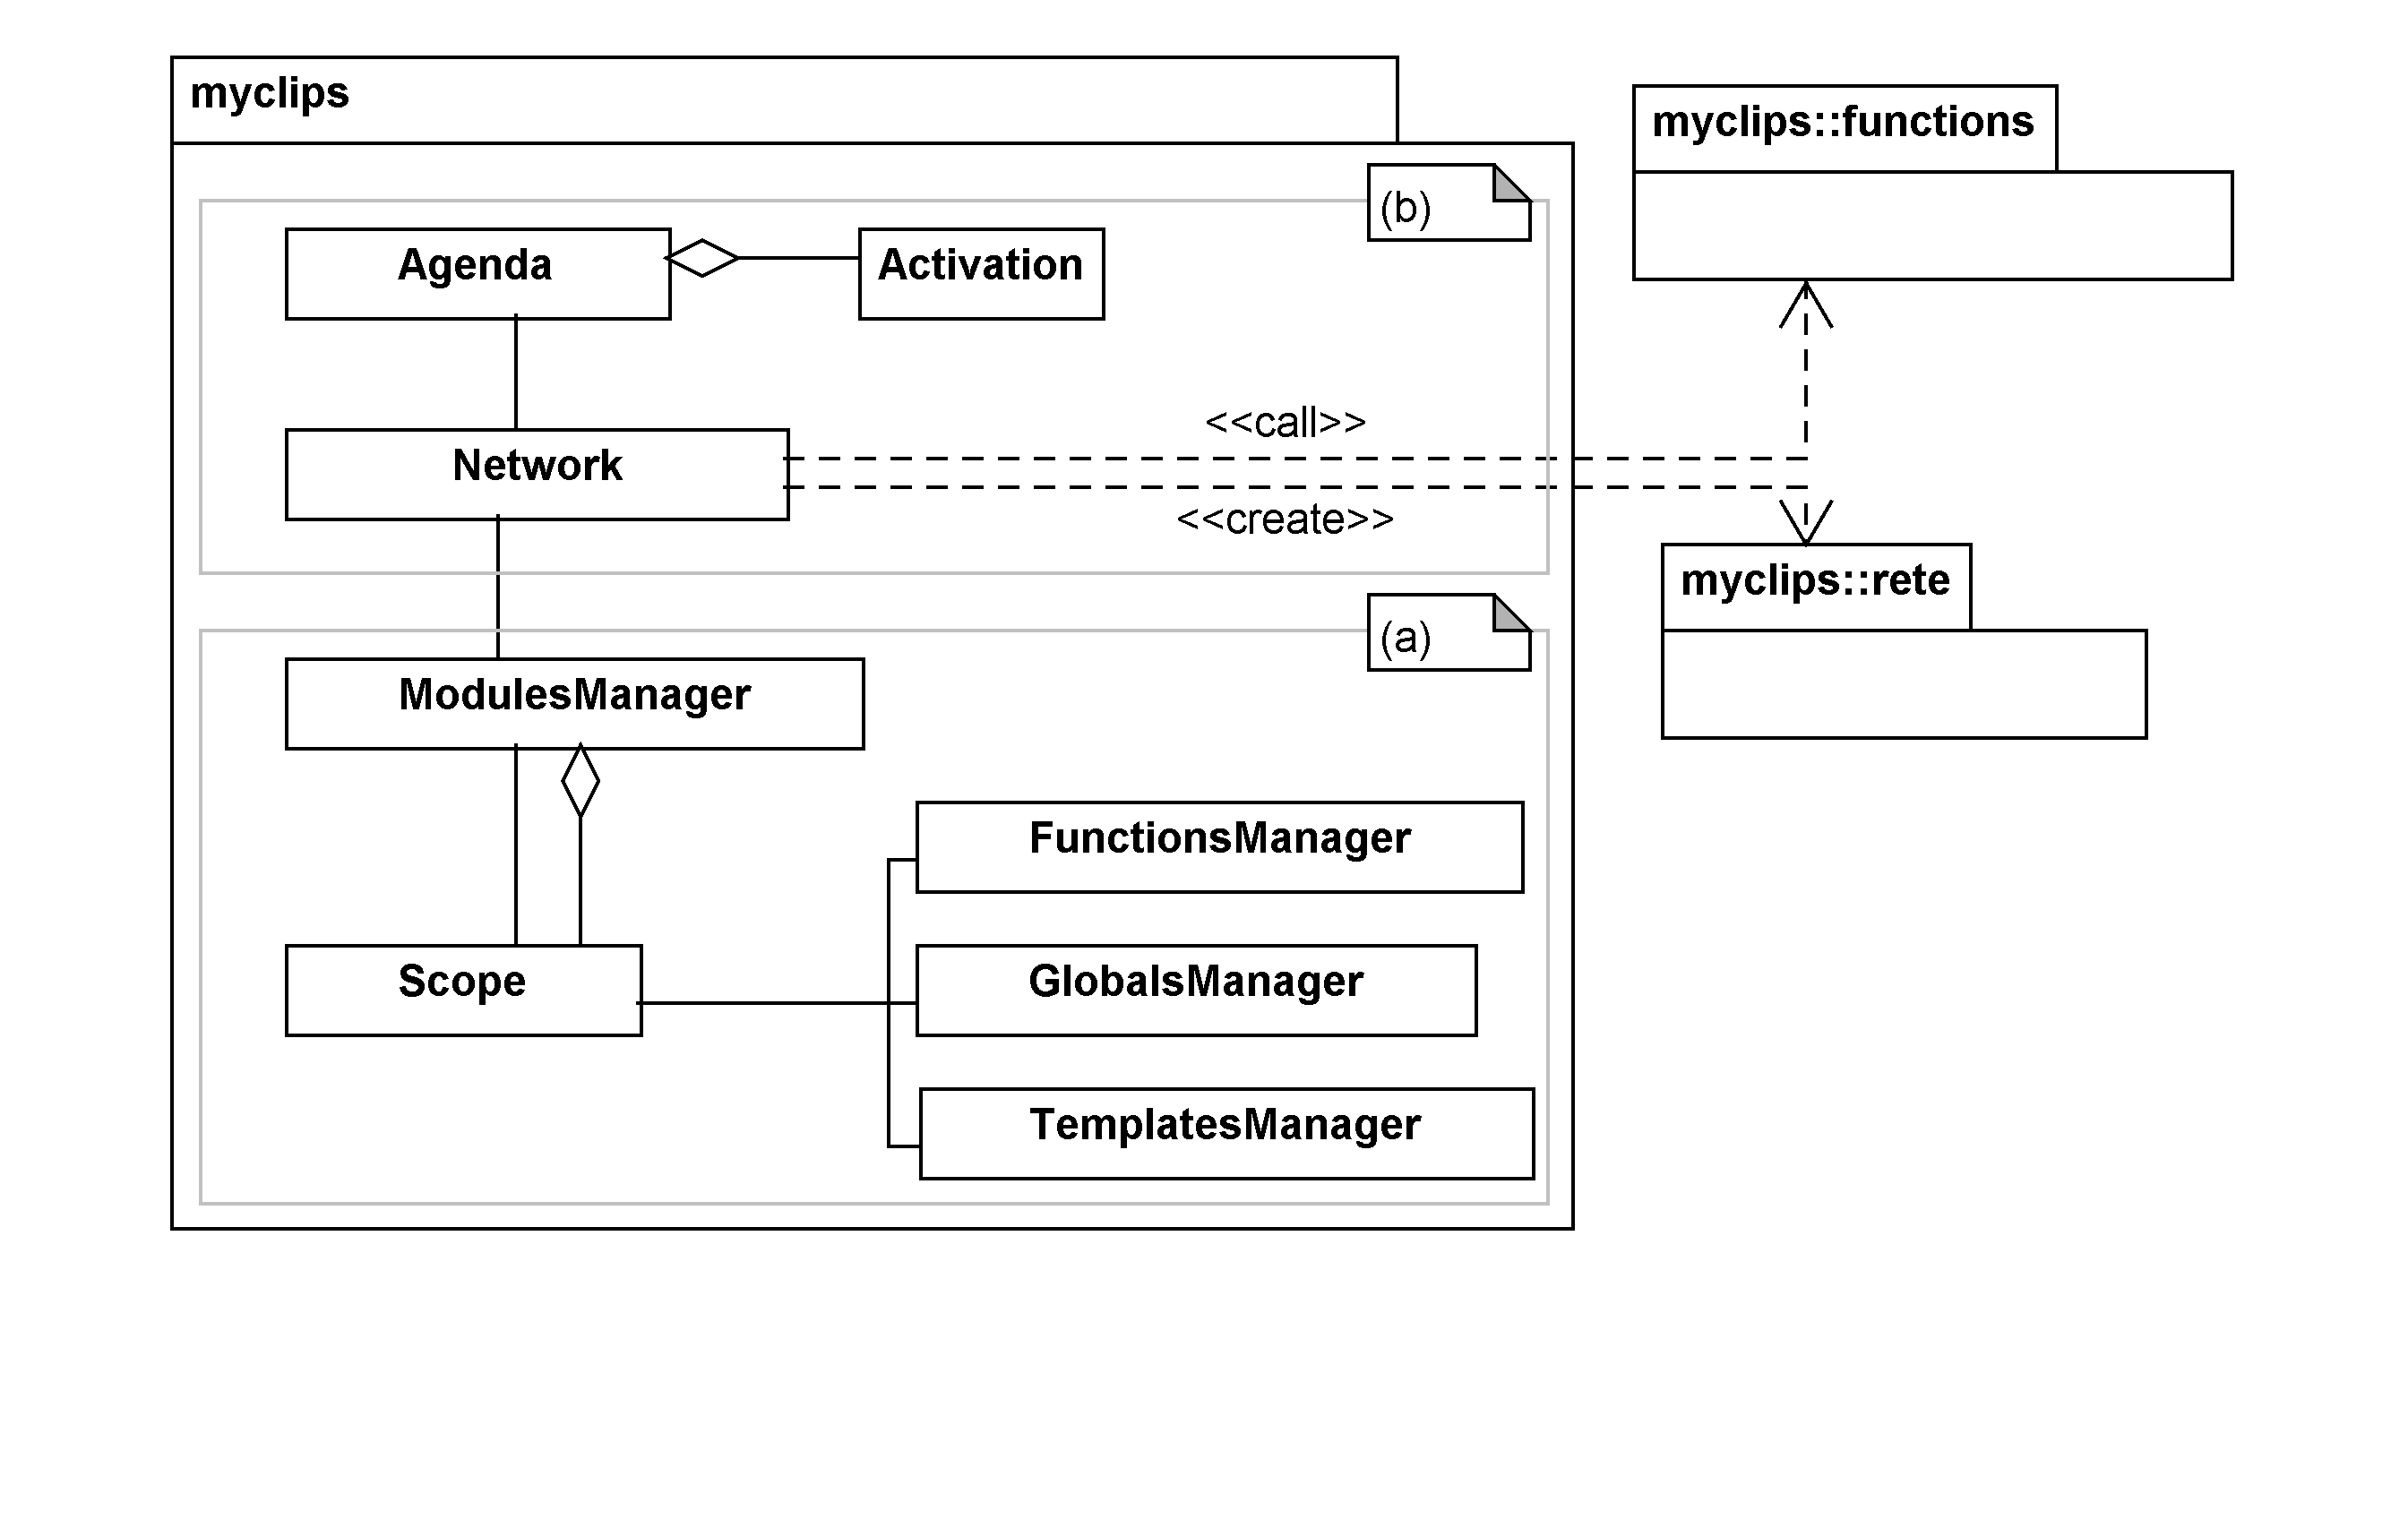
\includegraphics[width=1\textwidth]{Immagini/Capitolo3/Packages/IE.png}
\caption{Package \emph{myclips}: vista degli elementi che collaborano per la realizzazione dei servizi dell'\emph{IE}}\label{fig:packages-ie}
\end{figure}

Il ruolo del modulo \emph{Motore Inferenziale} (IE) è quello di offrire i servizi principali relativi alla gestione delle definizioni, all'esecuzione del ciclo \emph{recognize-act} e alla gestione delle transizioni fra gli stati del sistema.

A livello logico, le classi che lo realizzano possono essere raggruppate in due sezioni: una prima adibita alla gestione delle definizioni del sistema esperto (\figurename~\ref{fig:packages-ie}a), una seconda alla interpretazione e esecuzione dei costrutti (\figurename~\ref{fig:packages-ie}b).

\begin{figure}[h]
\centering
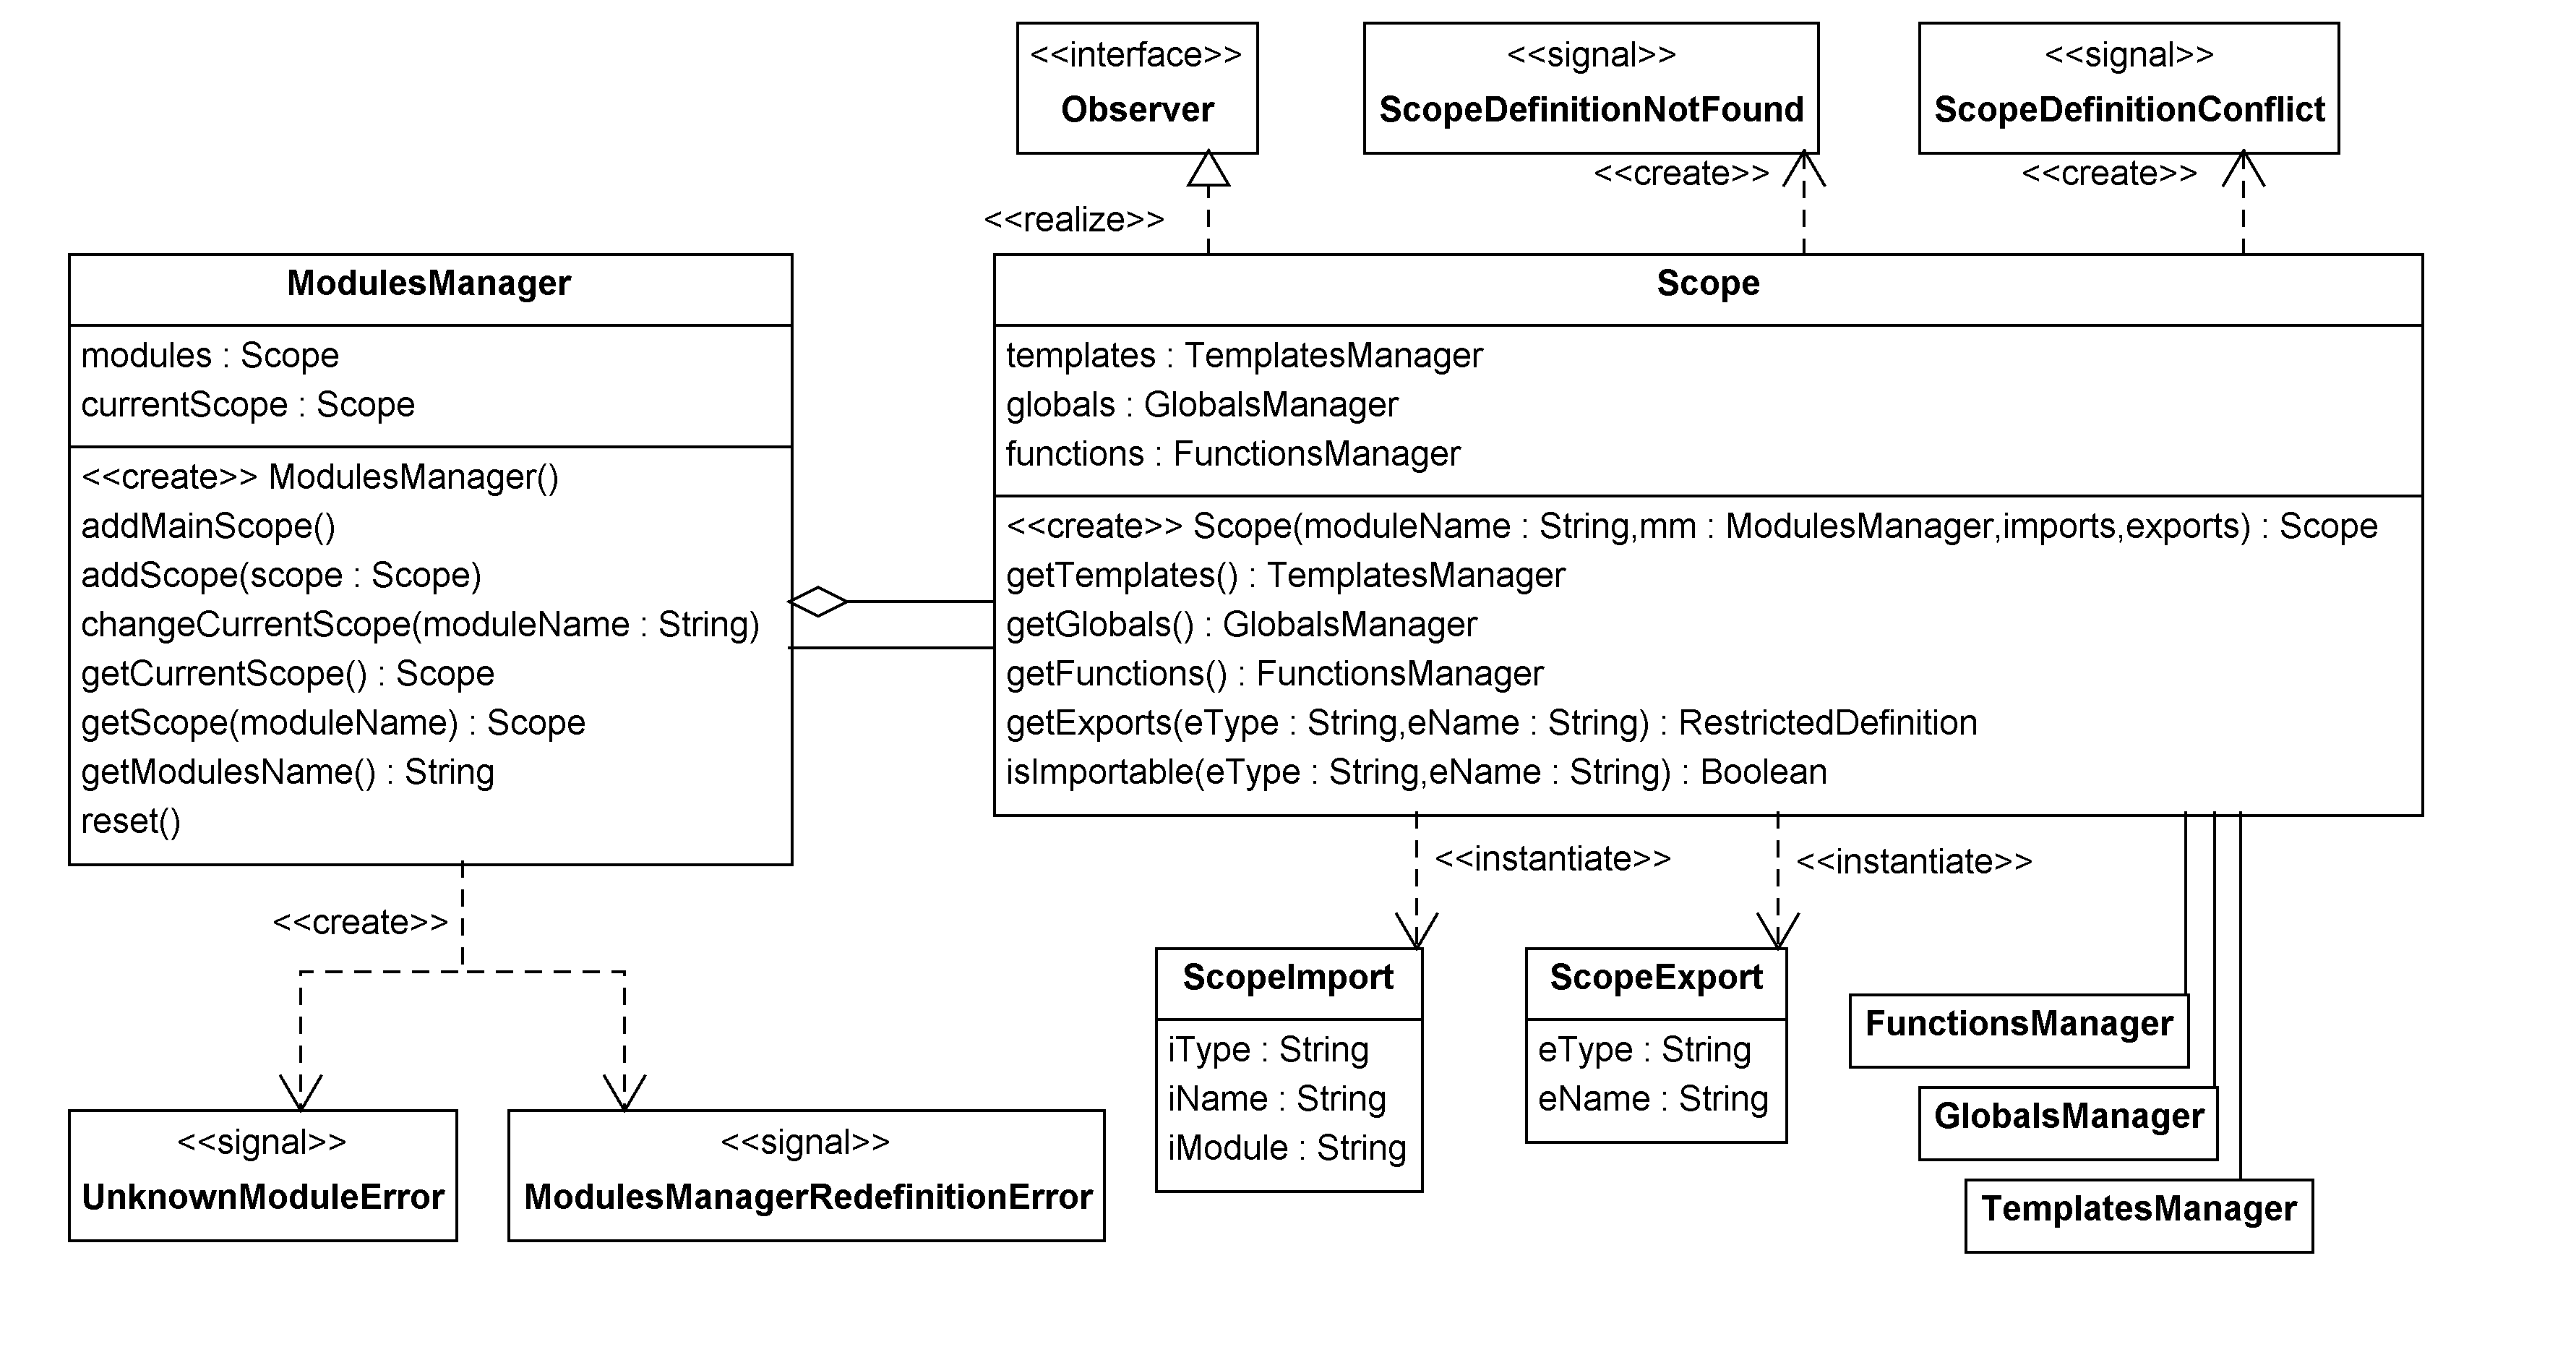
\includegraphics[width=1\textwidth]{Immagini/Capitolo3/Classi/myclips_Scope-ModulesManager.png}
\caption{Package \emph{myclips}: vista delle classi per la gestione dei moduli}\label{fig:class-myclips-scope-mm}
\end{figure}


\paragraph{Gestione delle definizioni}

La gestione dei moduli è affidata alla collaborazione fra le classi \emph{Scope} e \emph{ModulesManager}~(\figurename~\ref{fig:class-myclips-scope-mm}).
La classe \emph{ModulesManager} memorizza l'insieme dei moduli definiti in un sistema esperto e un attributo di stato (\emph{currentScope}) nel quale viene memorizzato il riferimento allo \emph{Scope} rappresentante il contesto corrente di esecuzione del sistema. Le definizioni o le azioni alle quali non è stato attribuito esplicitamente un modulo di appartenenza vengono automaticamente relazionate con il modulo corrente.

Le istanze di classe \emph{Scope} rappresentano singoli moduli definiti nel sistema. A differenza dell'entità \emph{modulo} intesa come collezione di costrutti e definizioni definiti nel \emph{modulo} stesso, quella di \emph{Scope} raggruppa l'insieme di definizioni disponibili in un preciso contesto d'uso relazionato ad un modulo. Ogni \emph{Scope} possiede i riferimenti ai manager dei tipi di costrutti definibili e gestisce il protocollo di \emph{import/export} delle definizioni~(\figurename~\ref{fig:sequence-def-import-export}).

\begin{figure}
\centering
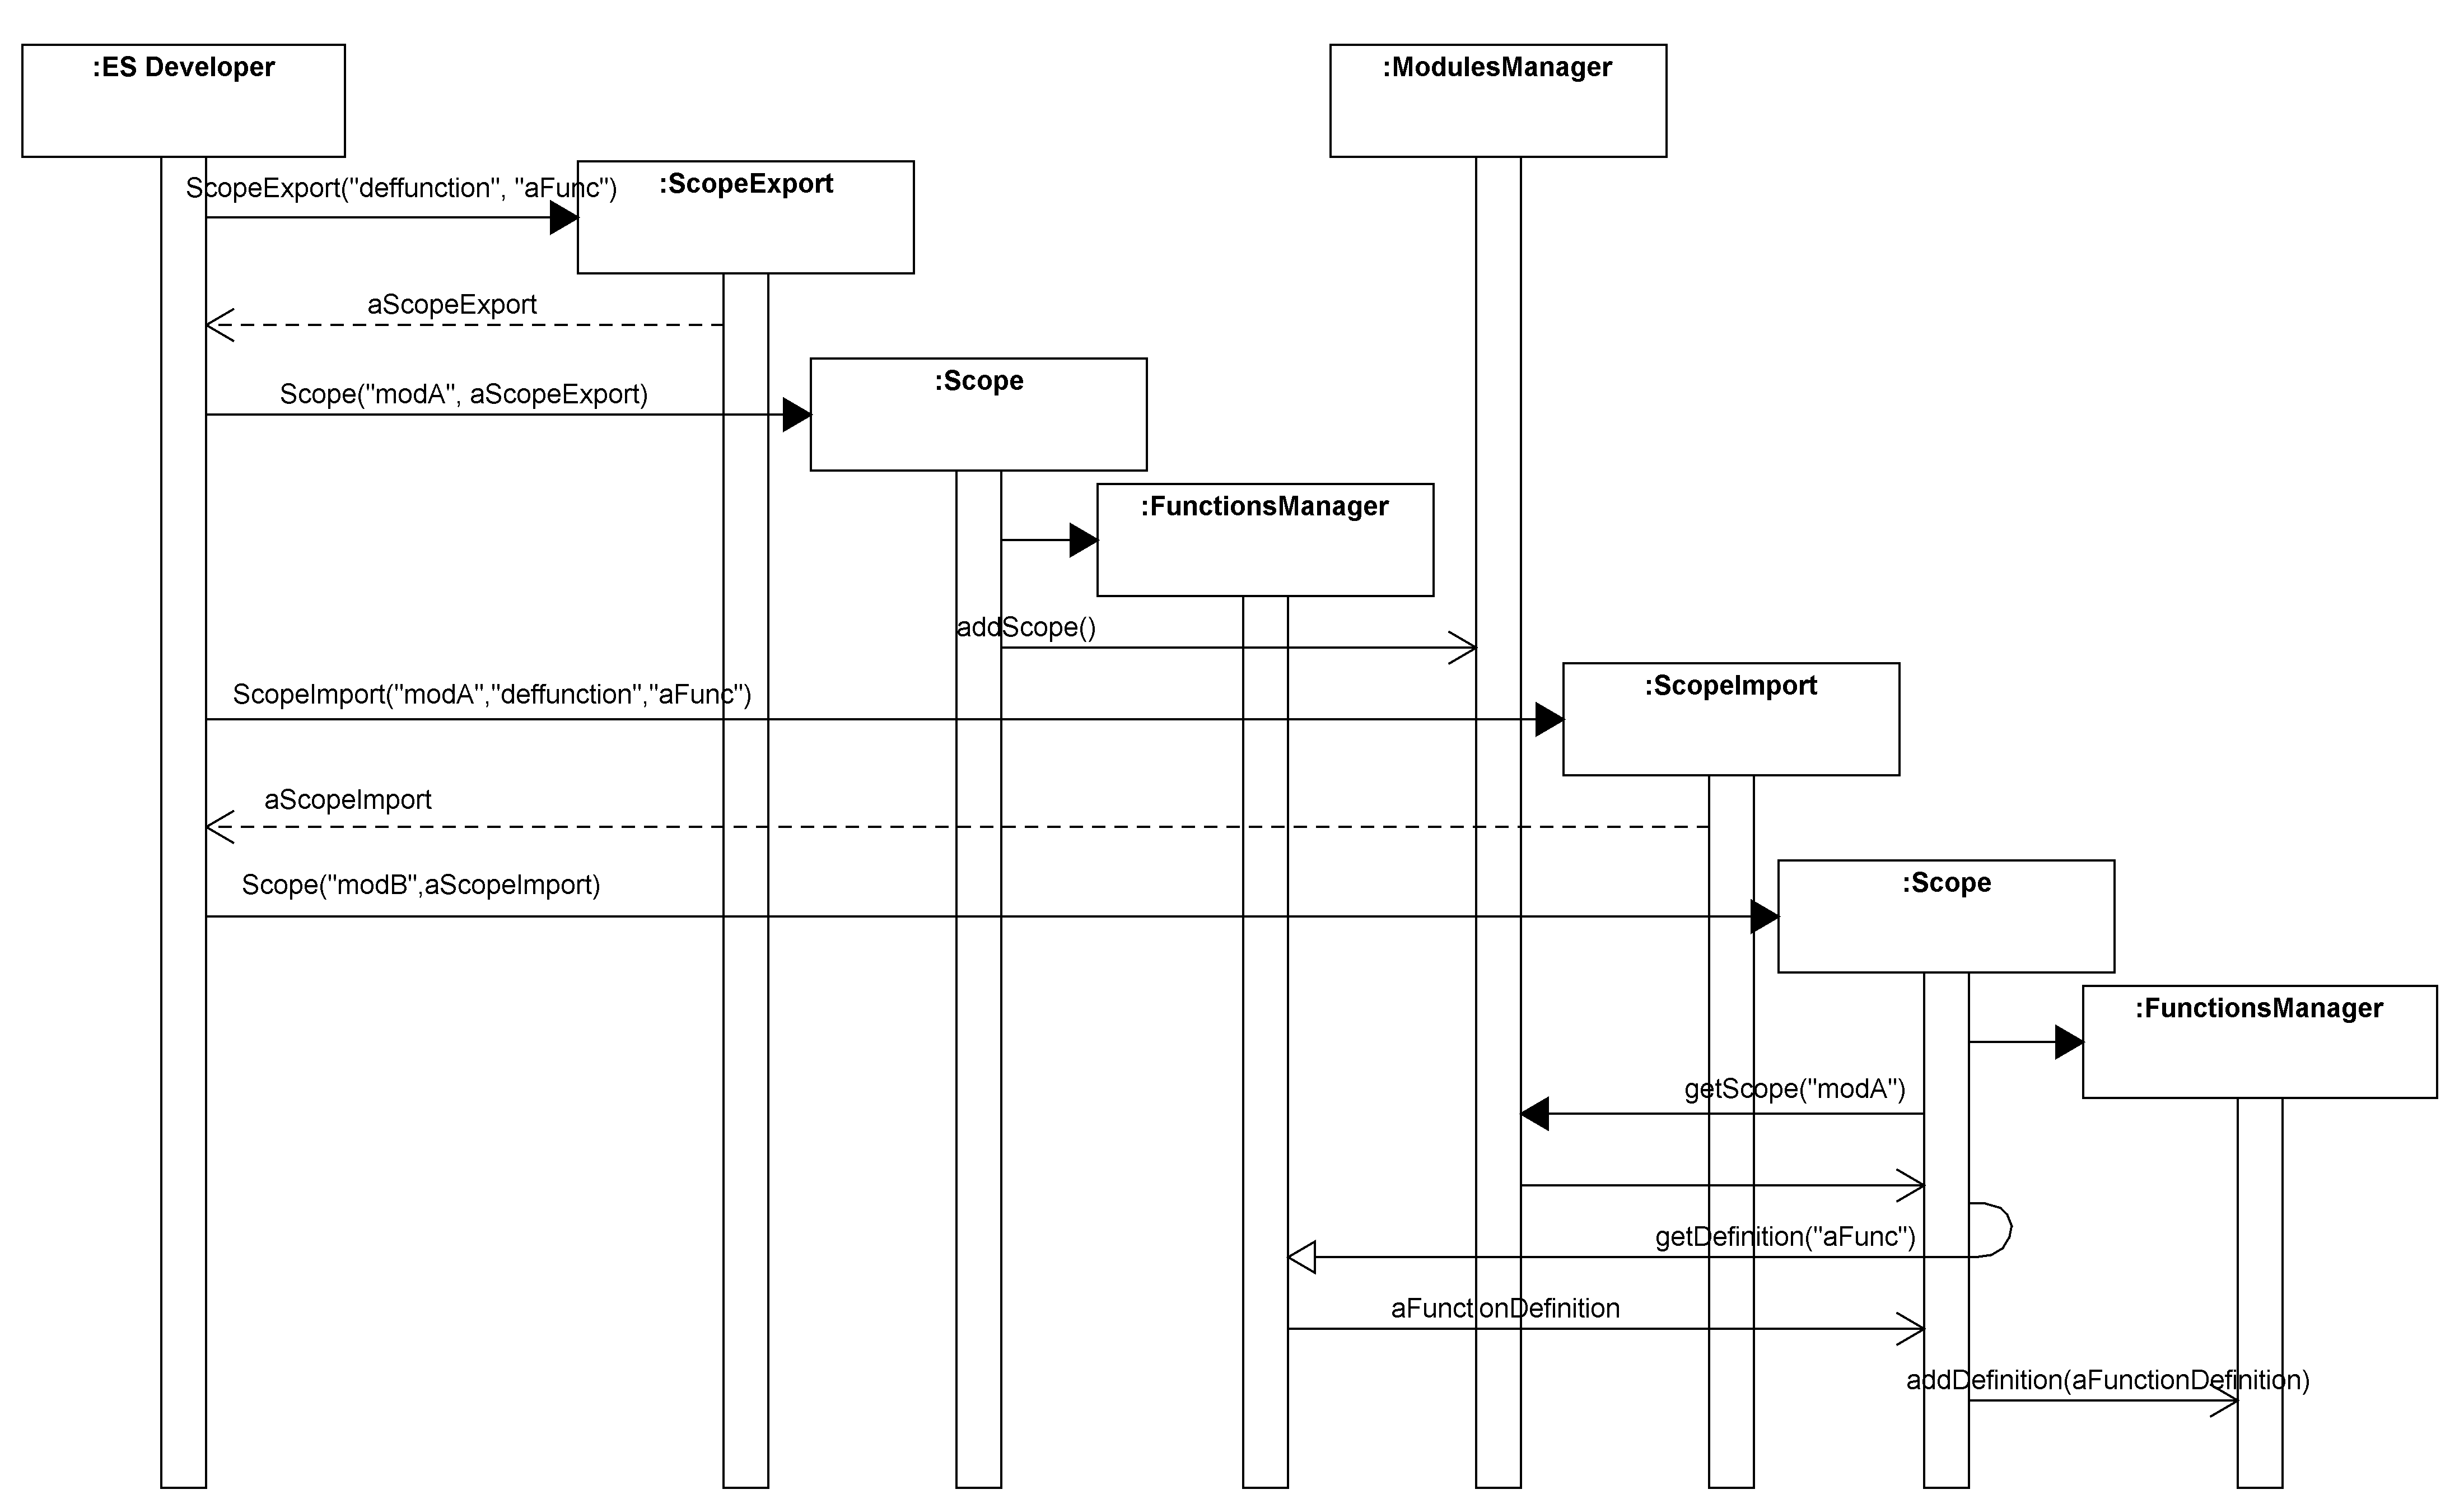
\includegraphics[width=1.2\textwidth, angle=270]{Immagini/Capitolo3/Sequenza/myclips_Scope_ImportExport.png}
\caption[Diagramma di sequenza \emph{import/export} delle definizioni]{Diagramma di sequenza \emph{import/export} delle definizioni: le clausule di importazione o esportazione determinano lo scambio di definizioni fra moduli}\label{fig:sequence-def-import-export}
\end{figure}

\begin{figure}
\centering
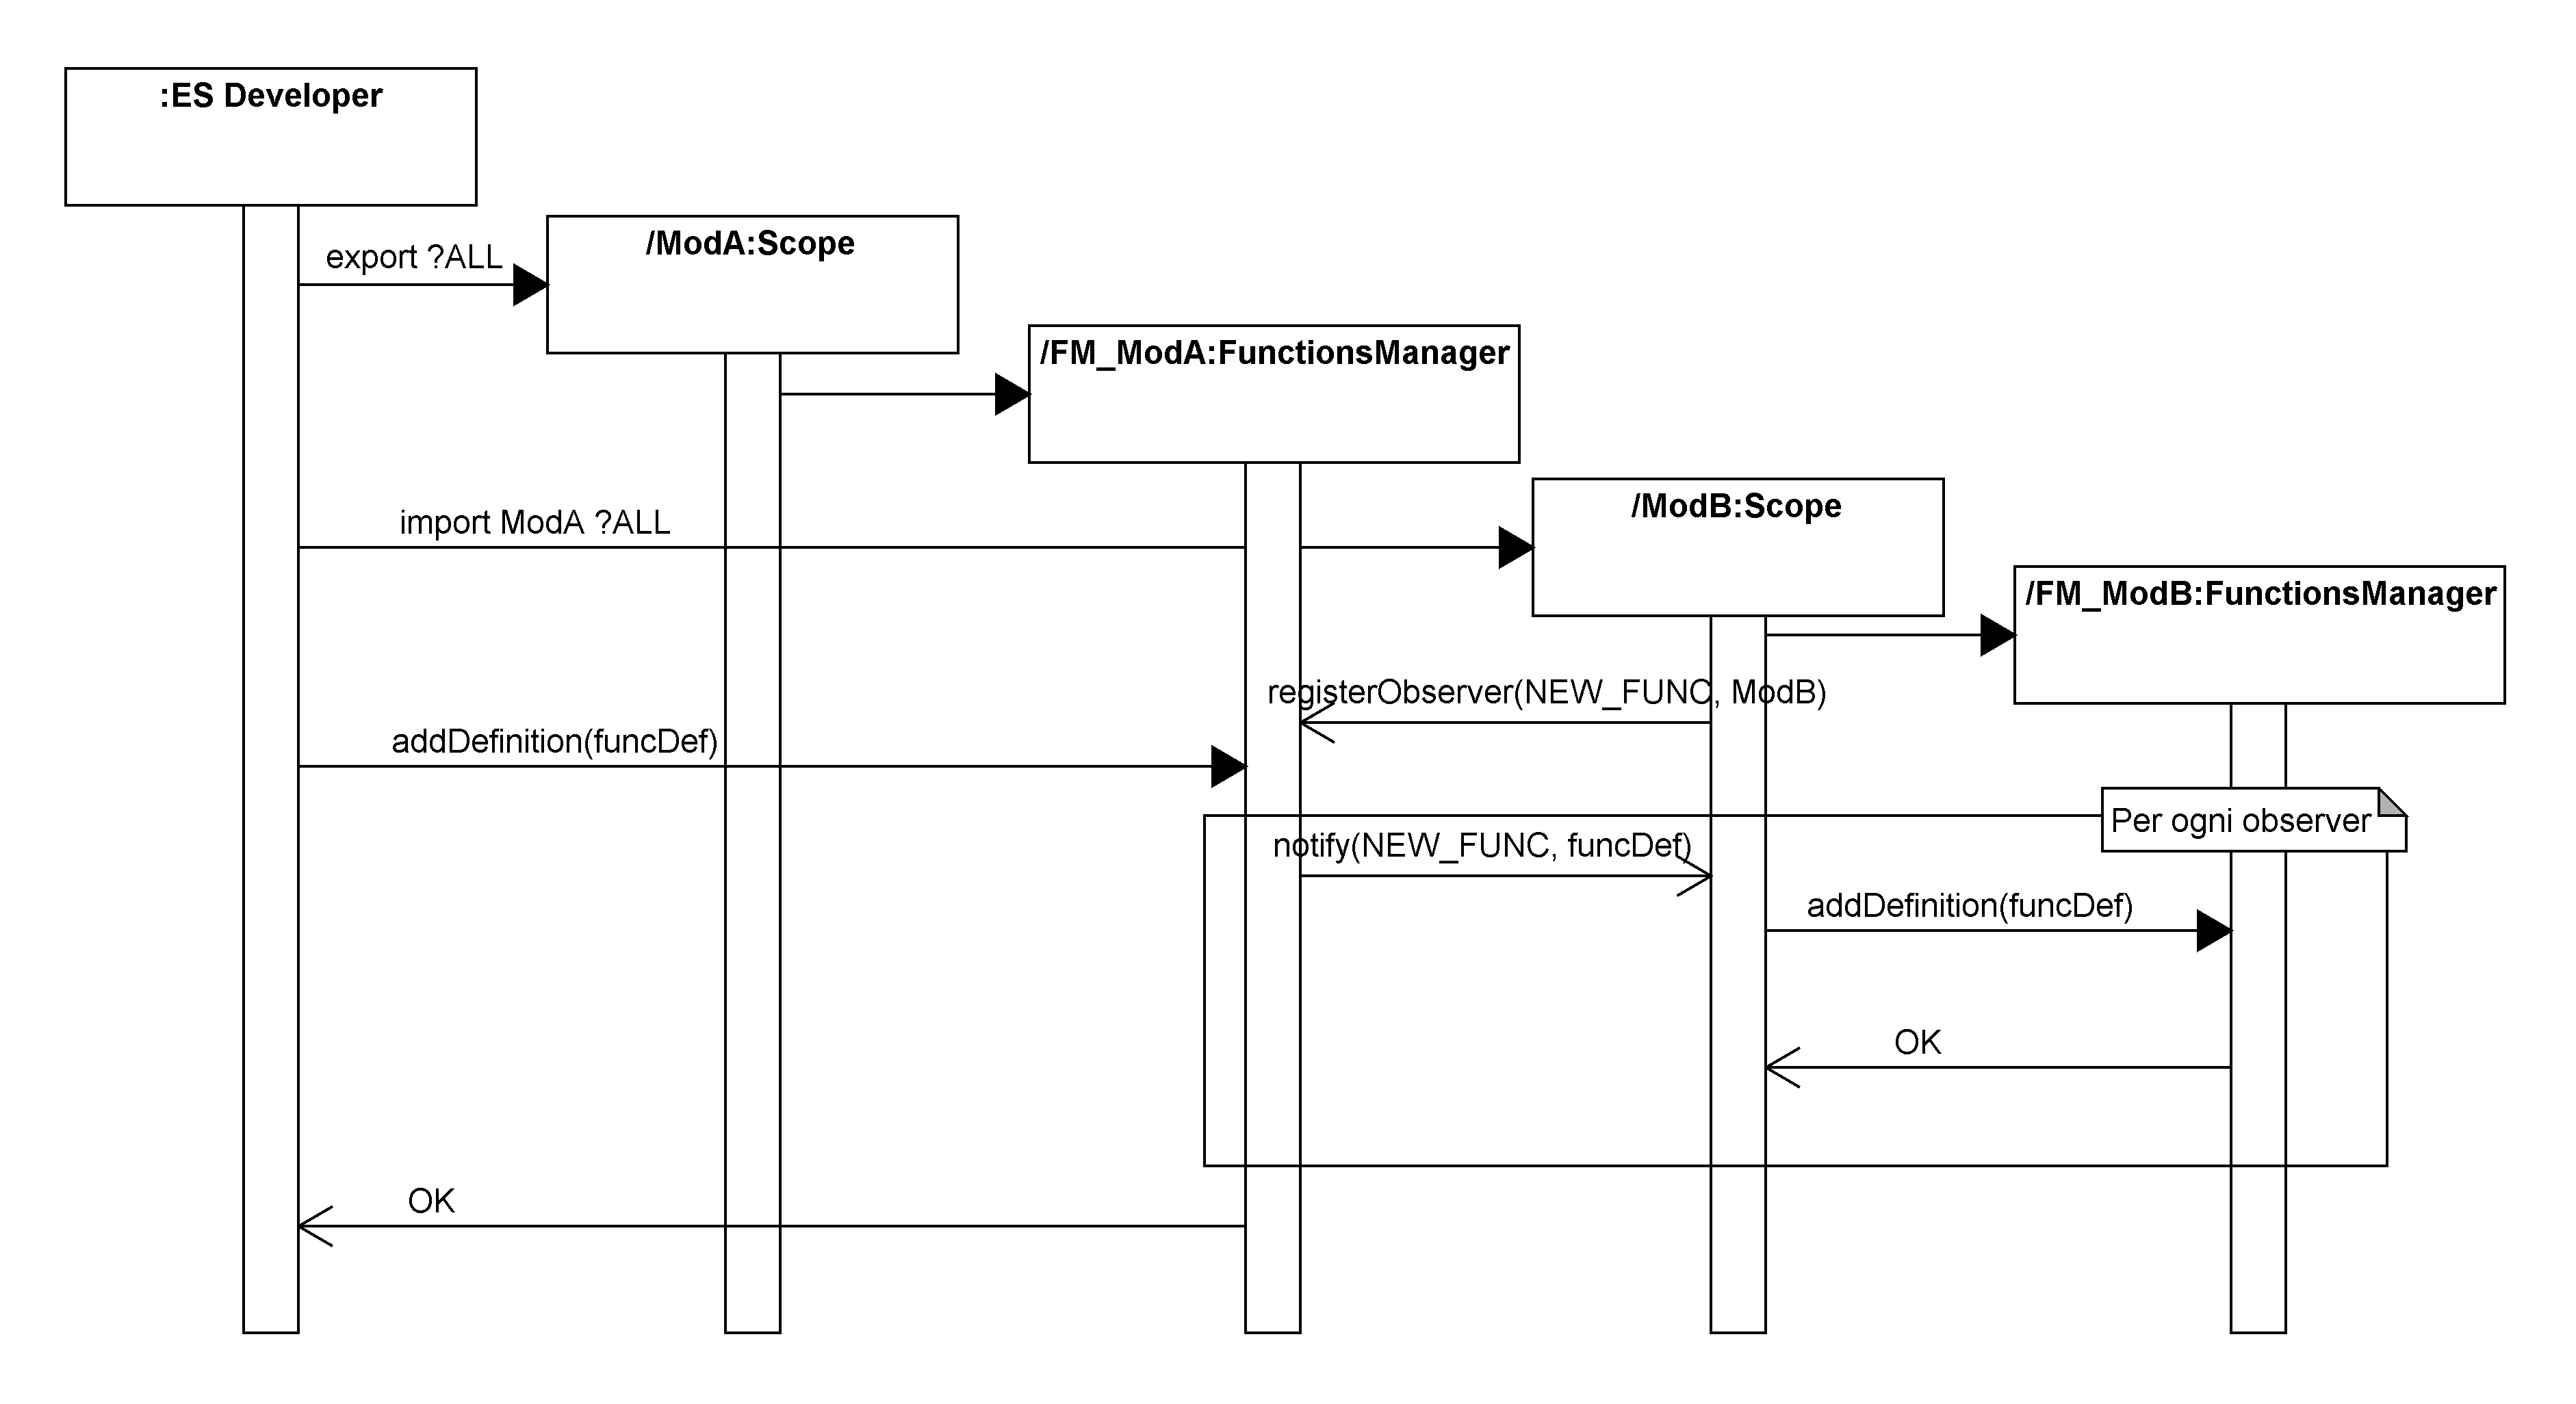
\includegraphics[width=1.3\textwidth, angle=270]{Immagini/Capitolo3/Sequenza/myclips_Scope_ExportPromise.png}
\caption[Diagramma di sequenza \emph{import/export} tramite l'uso di \emph{promesse}]{Diagramma di sequenza \emph{import/export} tramite l'uso di \emph{promesse}: i moduli vengono relazionati e l'aggiunta successiva di definizioni al primo modulo viene automaticamente inoltrata al secondo modulo}\label{fig:sequence-def-import-export-promise}
\end{figure}

Lo scambio di definizioni non ancora esplicitate avviene attraverso l'utilizzo delle \emph{promesse di import/export}. Nel momento in cui un modulo \emph{modA} definisce tutti i propri costrutti esportabili ed un secondo modulo \emph{modB} esplicita la volontà di importare tutti i costrutti di \emph{modA}, si fa uso di una \emph{promessa}: il protocollo prevede l'utilizzo di una soluzione basata sul pattern \emph{observer-observable} per eseguire il trasferimento delle definizioni aggiunte in fasi successive~(\figurename~\ref{fig:sequence-def-import-export-promise}).

\begin{figure}
\centering
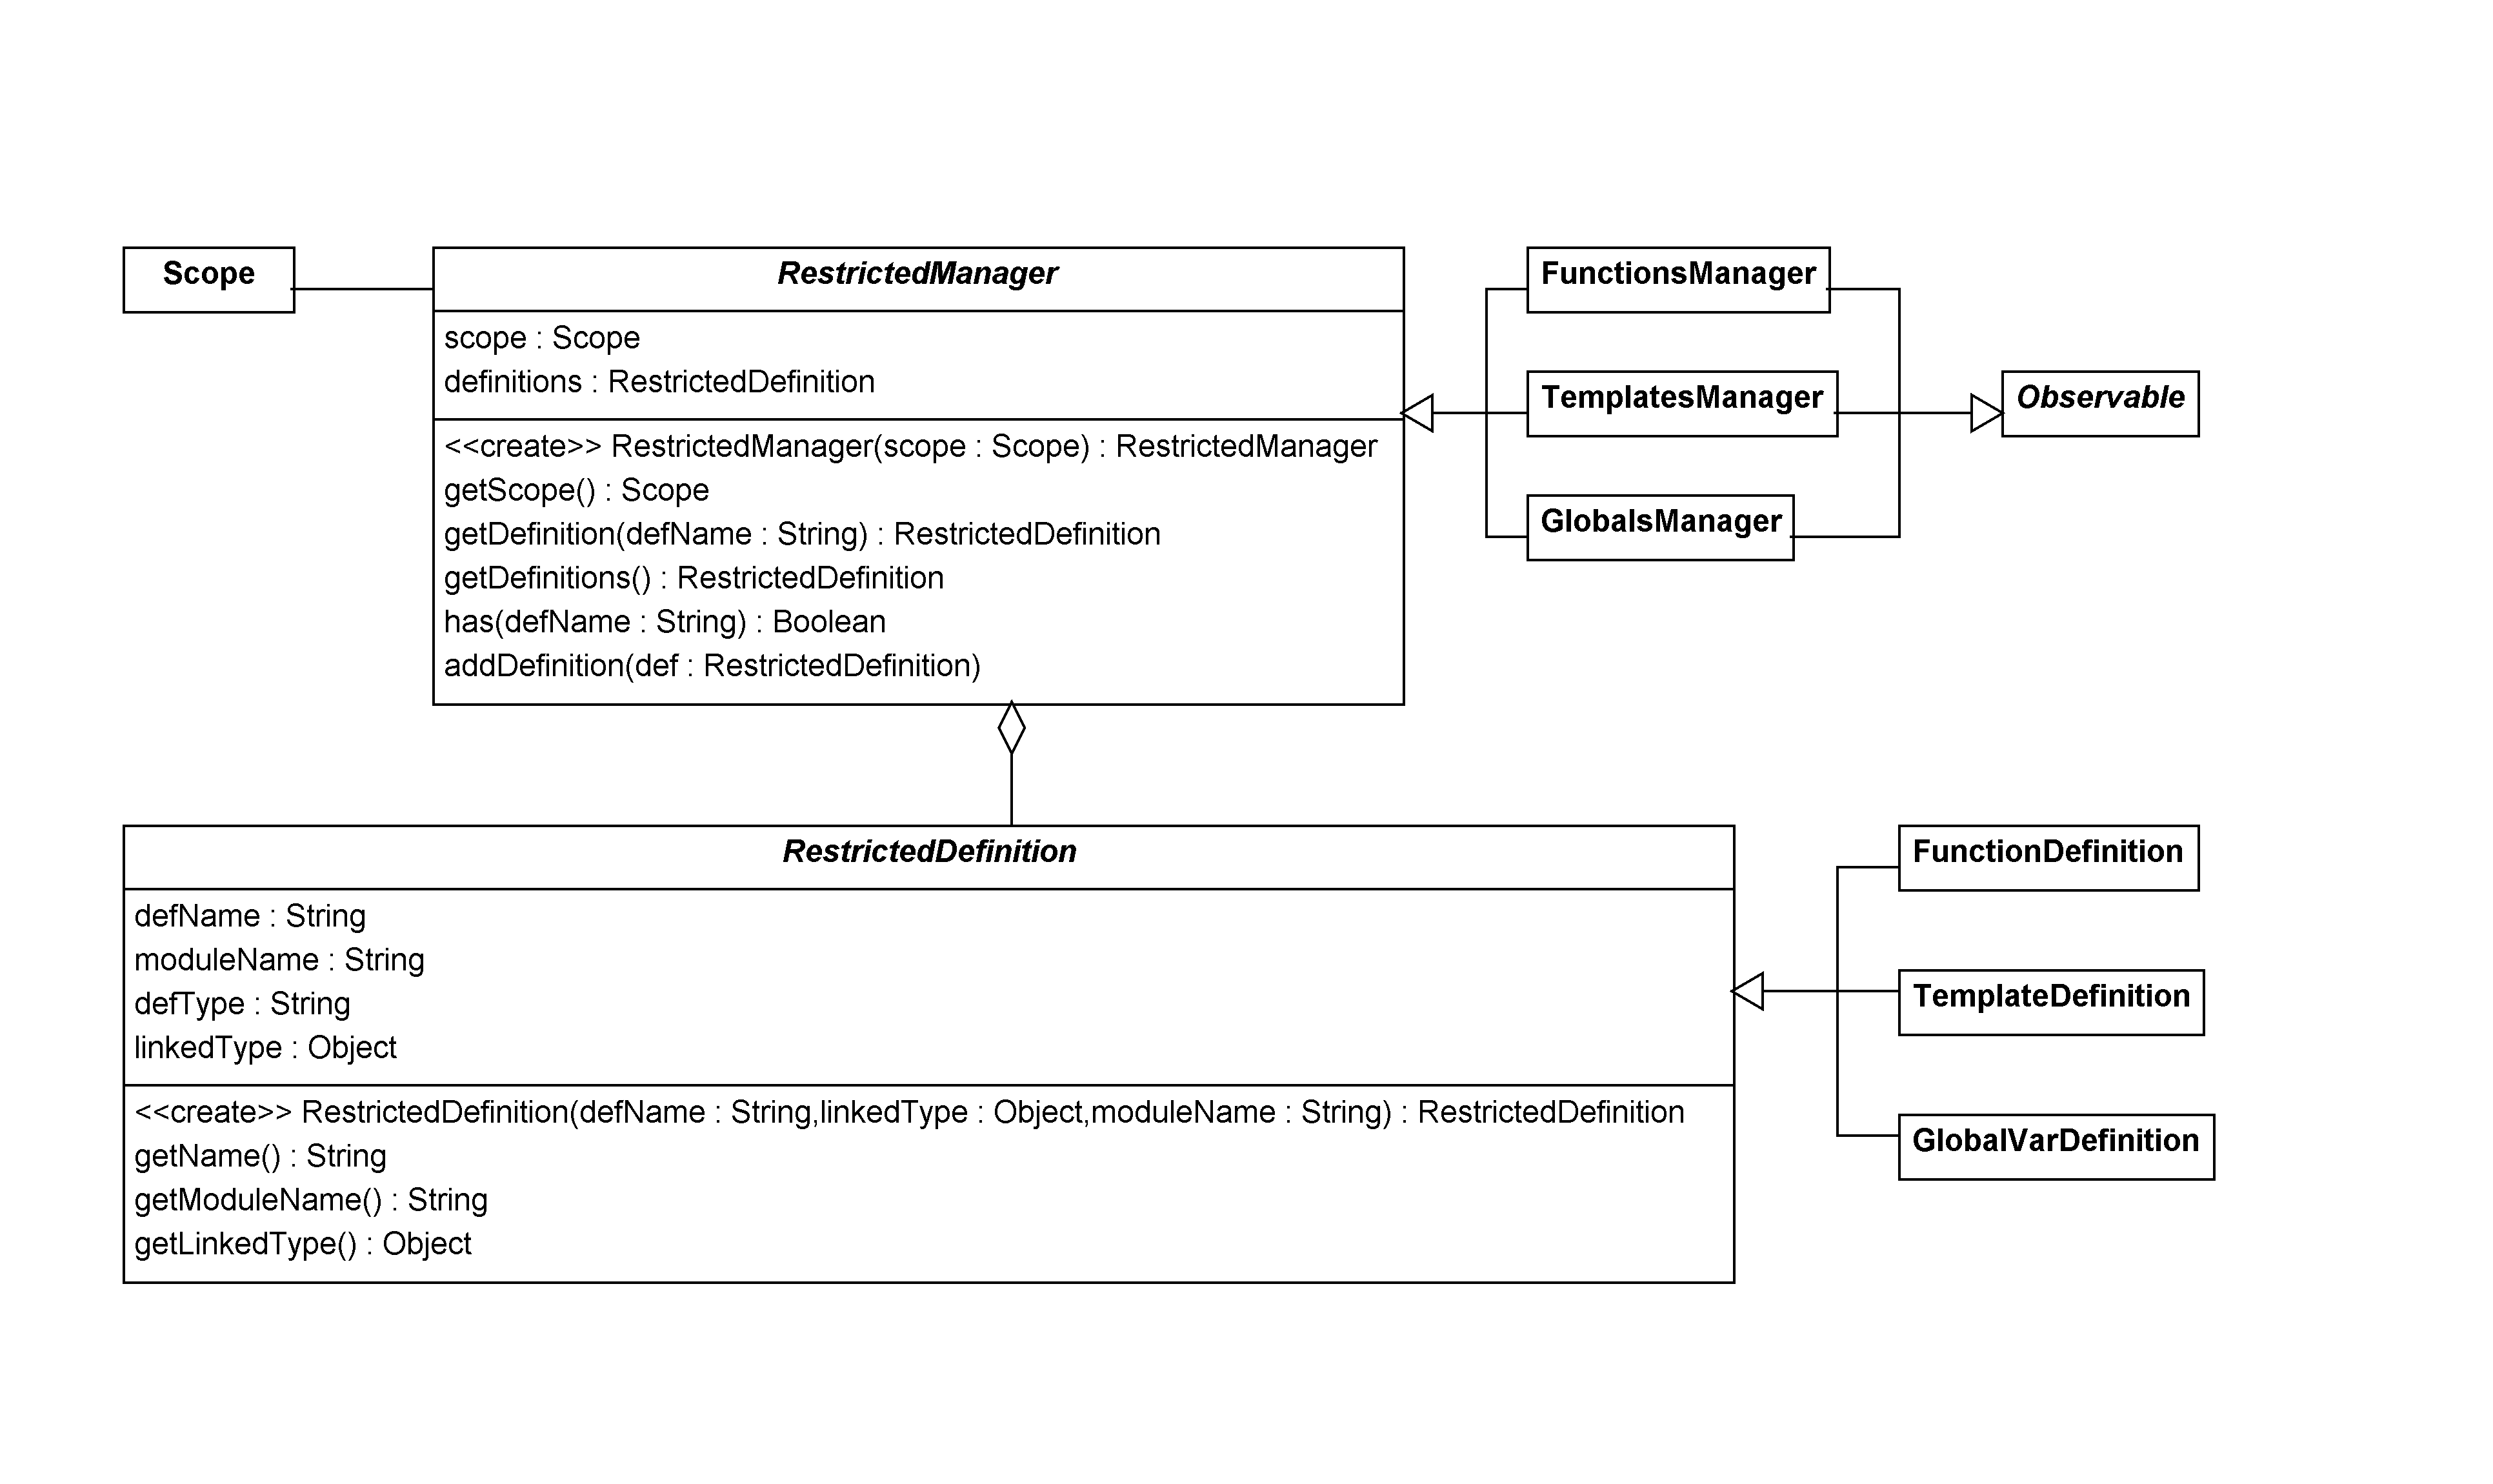
\includegraphics[width=1\textwidth]{Immagini/Capitolo3/Classi/myclips_RestrictedManager.png}
\caption{Vista delle classi \emph{manager} di definizioni}\label{fig:class-myclips-restricted-manager}
\end{figure}

La memorizzazione delle definizioni è affidata alle classi \emph{GlobalsManager}, \emph{TemplatesManager} e \emph{FunctionsManager}~(\figurename~\ref{fig:class-myclips-restricted-manager}). 
Ogni \emph{manager} memorizza un preciso tipo di definizioni che possono essere utilizzate nell'ambito di uno \emph{Scope} specifico. L'eventuale presenza di \emph{promesse di export} viene valutata durante l'aggiunta di nuove definizioni nei \emph{manager}~(\figurename~\ref{fig:sequence-def-import-export-promise}).

\clearpage

\paragraph{Gestione dell'inferenza}

\begin{figure}
\centering
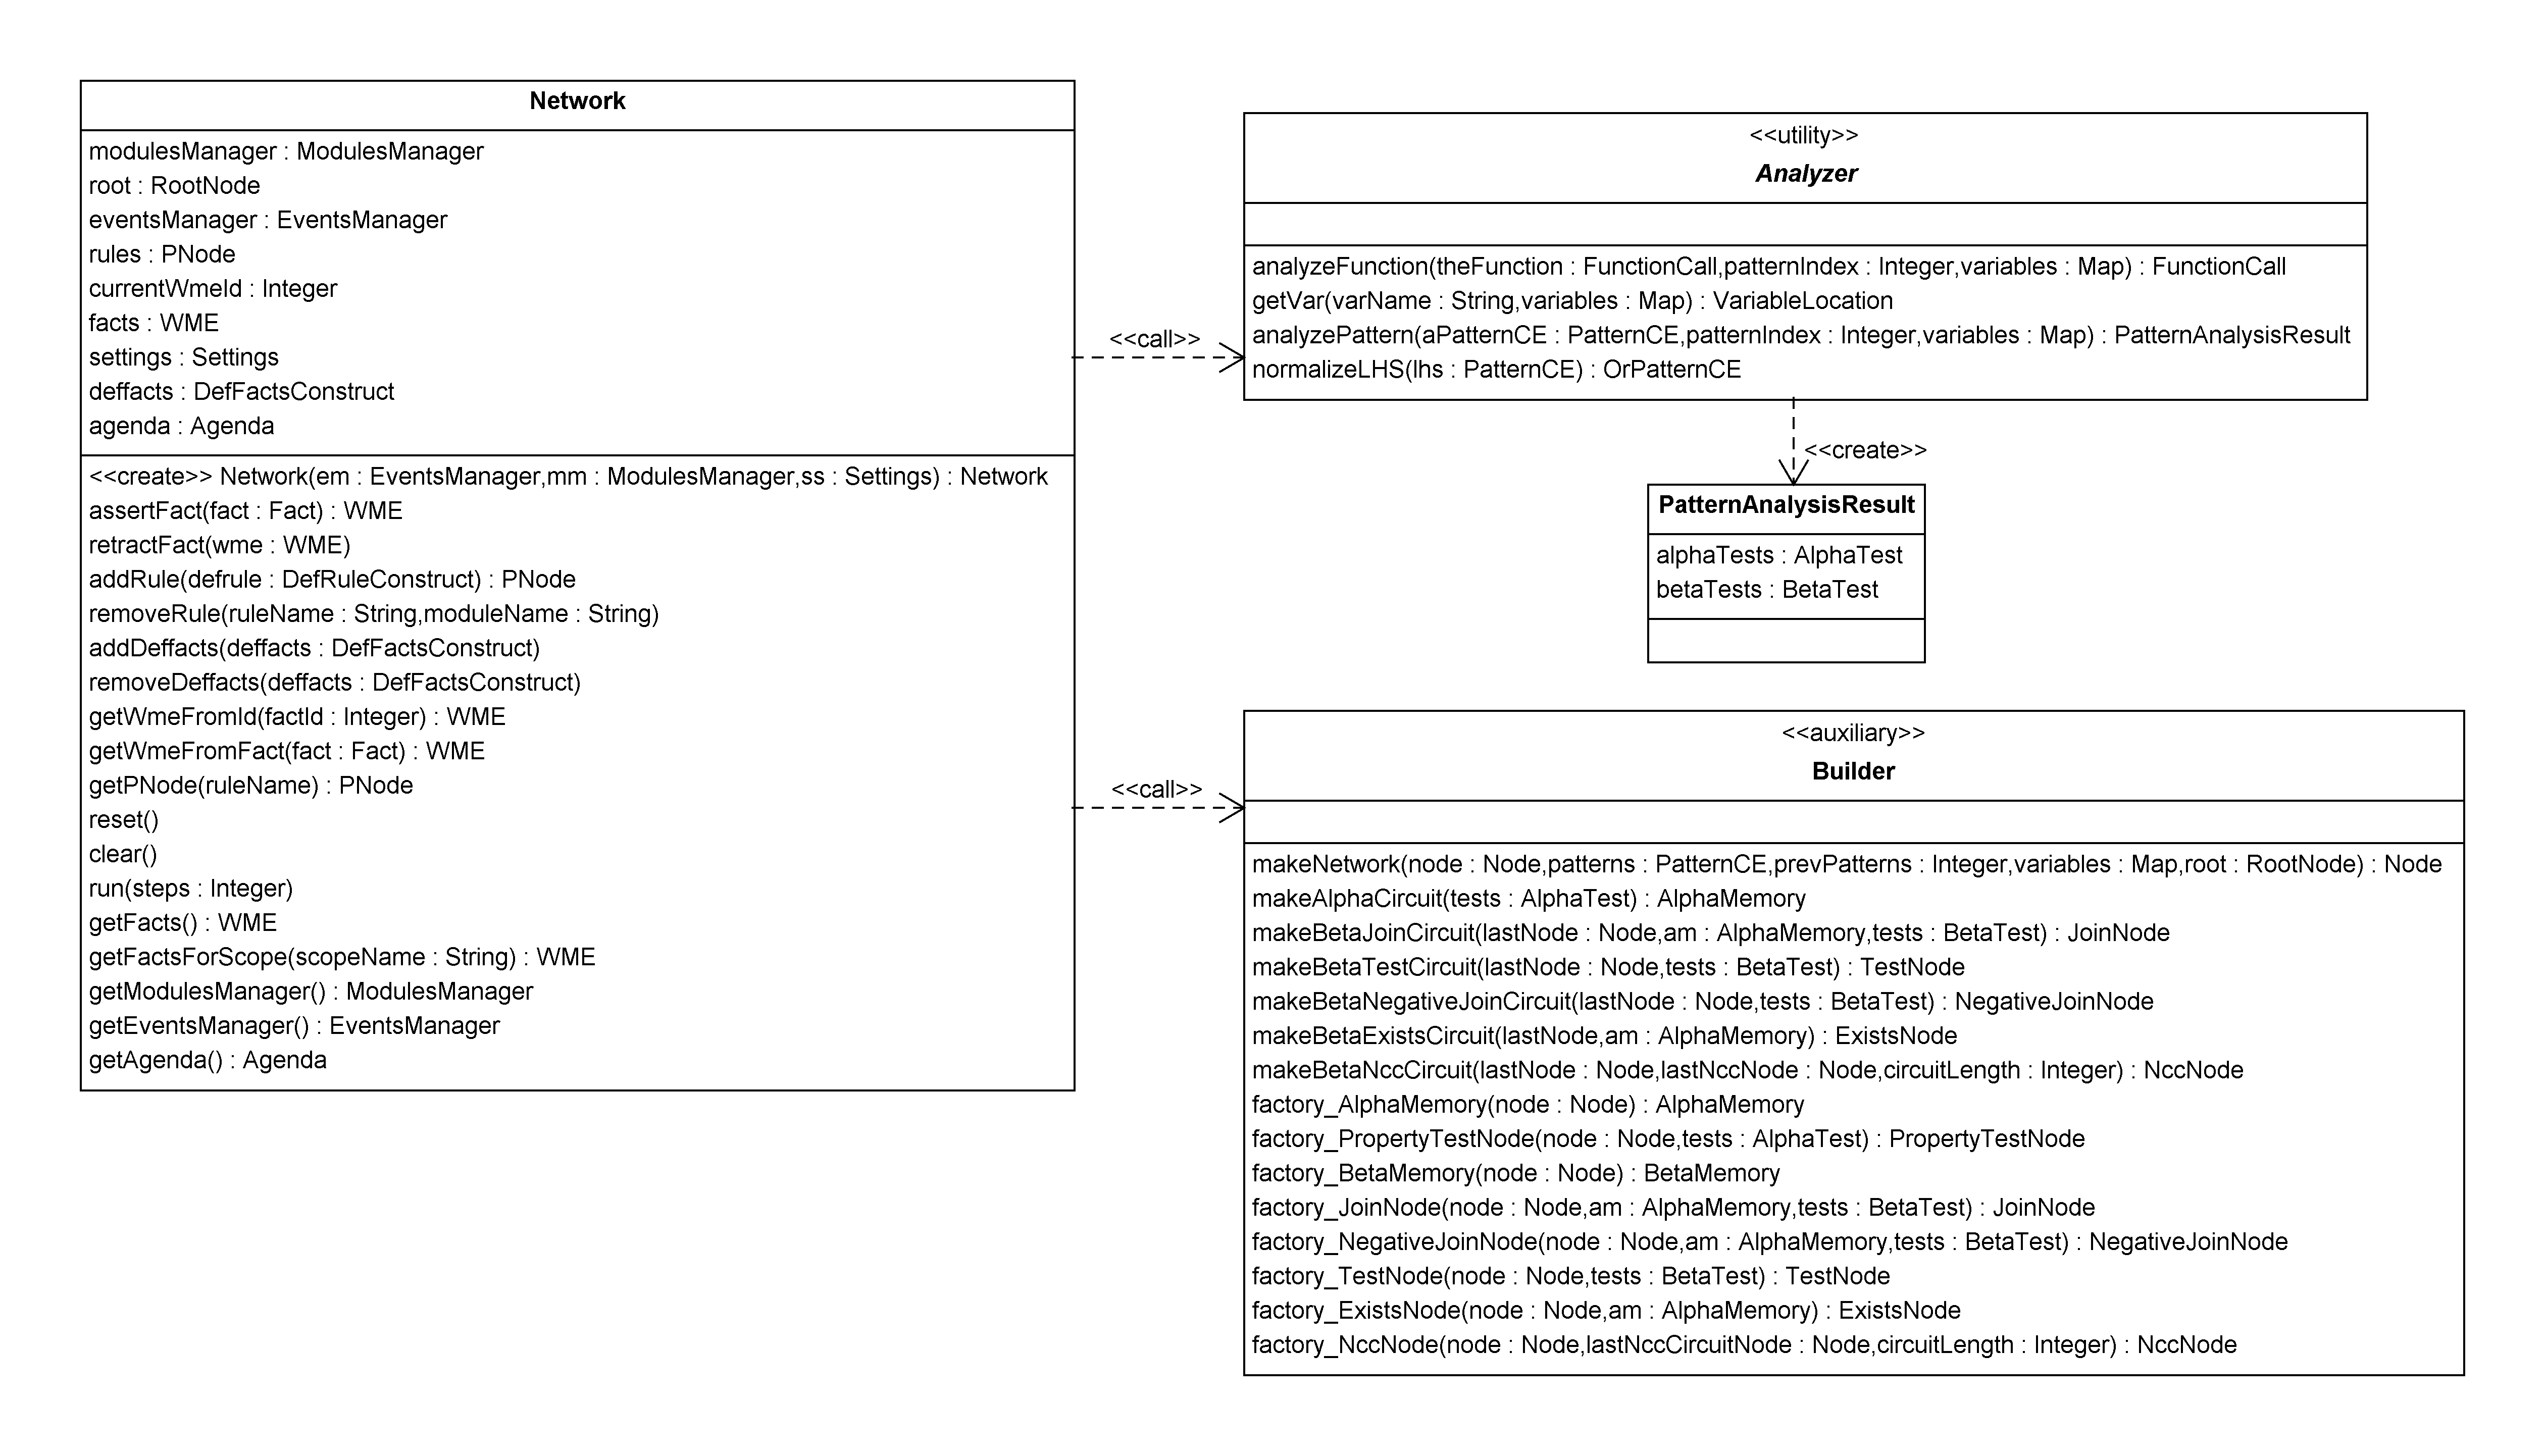
\includegraphics[width=0.9\textwidth]{Immagini/Capitolo3/Classi/myclips_rete_Network.png}
\caption{Package \emph{myclips}: vista della classe \emph{Network}}\label{fig:class-myclips-network}
\end{figure}

La classe principale per la gestione dell'inferenza è la classe \emph{fa\c{c}ade} \emph{Network}~(\figurename~\ref{fig:class-myclips-network}): astraendo dalla complessità delle interfacce offerte dal \emph{matcher}, offre metodi per la manipolazione del \emph{rules-set}, dei fatti iniziali e della \emph{working-memory}. Realizzando il ciclo \emph{recognize-act} al suo interno, permette l'utilizzo dei meccanismi di inferenza offerti dal sistema. La classe si affida a due componenti \emph{utility} per la reale implementazione delle funzionalità di compilazione e analisi delle regole interfacciandosi con il modulo \emph{matcher}, descritto in seguito.


\begin{figure}
\centering
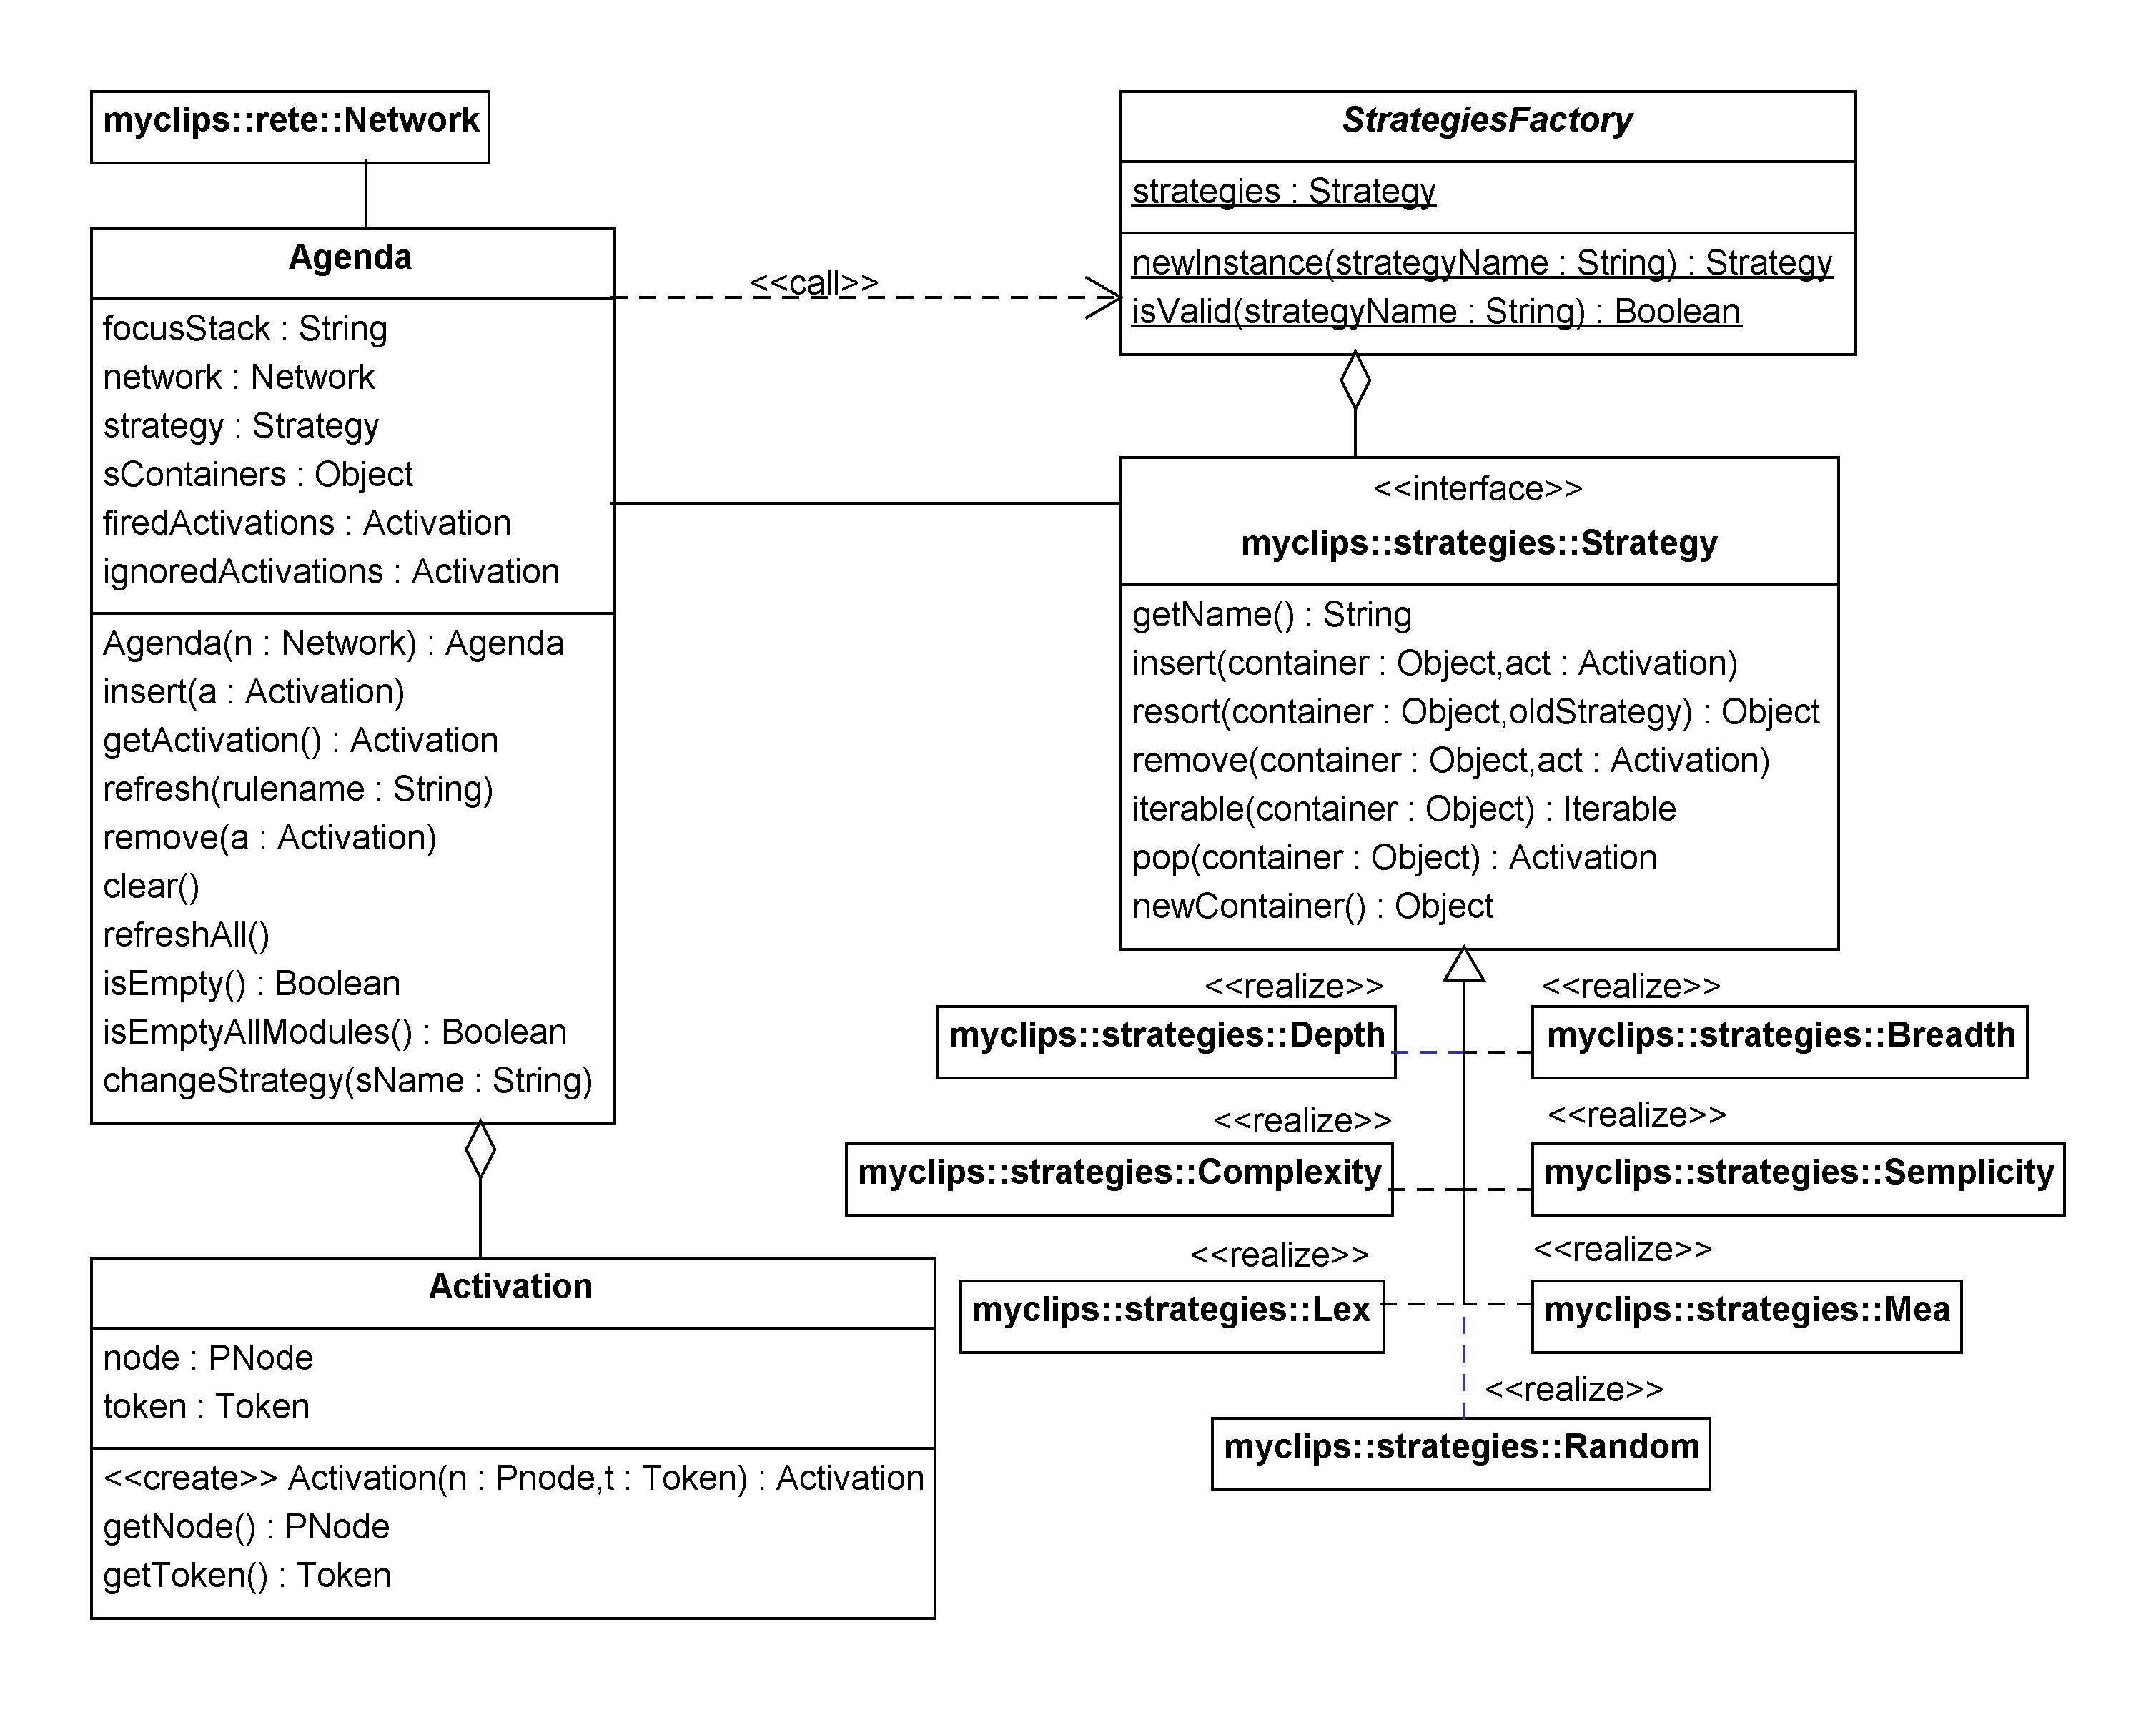
\includegraphics[width=0.9\textwidth]{Immagini/Capitolo3/Classi/myclips_Agenda-Strategies.png}
\caption{Package \emph{myclips}: vista delle classi e interfacce relative ad  \emph{Agenda} e \emph{Strategie} (CRS)}\label{fig:class-myclips-agenda-strategies}
\end{figure}

La gestione delle attivazioni viene affidata alla classe \emph{Agenda} e al \emph{package} \emph{myclips.strategies}~(\figurename~\ref{fig:class-myclips-agenda-strategies}). La classe organizza le attivazioni, offrendo servizi per l'aggiunta o la rimozione delle stesse, e gestendo le strategie di risoluzione dei conflitti. La collaborazione fra \emph{Agenda} e \emph{Strategy} viene realizzata attraverso l'utilizzo del pattern \emph{Factory}: la creazione dell'istanza di strategia viene delegata ad una istanza \emph{Singleton} della classe \emph{StrategiesFactory}, la quale inizializza un'implementazione dell'interfaccia \emph{Strategy} fornita basandosi su un id di strategia. L'implementazione dell'\emph{Agenda} viene realizzata tenendo conto dei metodi forniti dall'interfaccia, astraendo dall'implementazione concreta. Le strutture dati adibite alla memorizzazione delle sequenze di attivazioni vengono inizializzate e concretamente gestite dalla specifica implementazione della \emph{Strategy}.

\clearpage


\subsubsection{Modulo Matcher}
Lo scopo del modulo \emph{matcher} è quello di confrontare lo stato della \emph{working-memory} con il \emph{rule-set}, identificando l'insieme di attivazioni disponibili e inserendole nell'\emph{agenda delle attivazioni}.

\begin{figure}
\centering
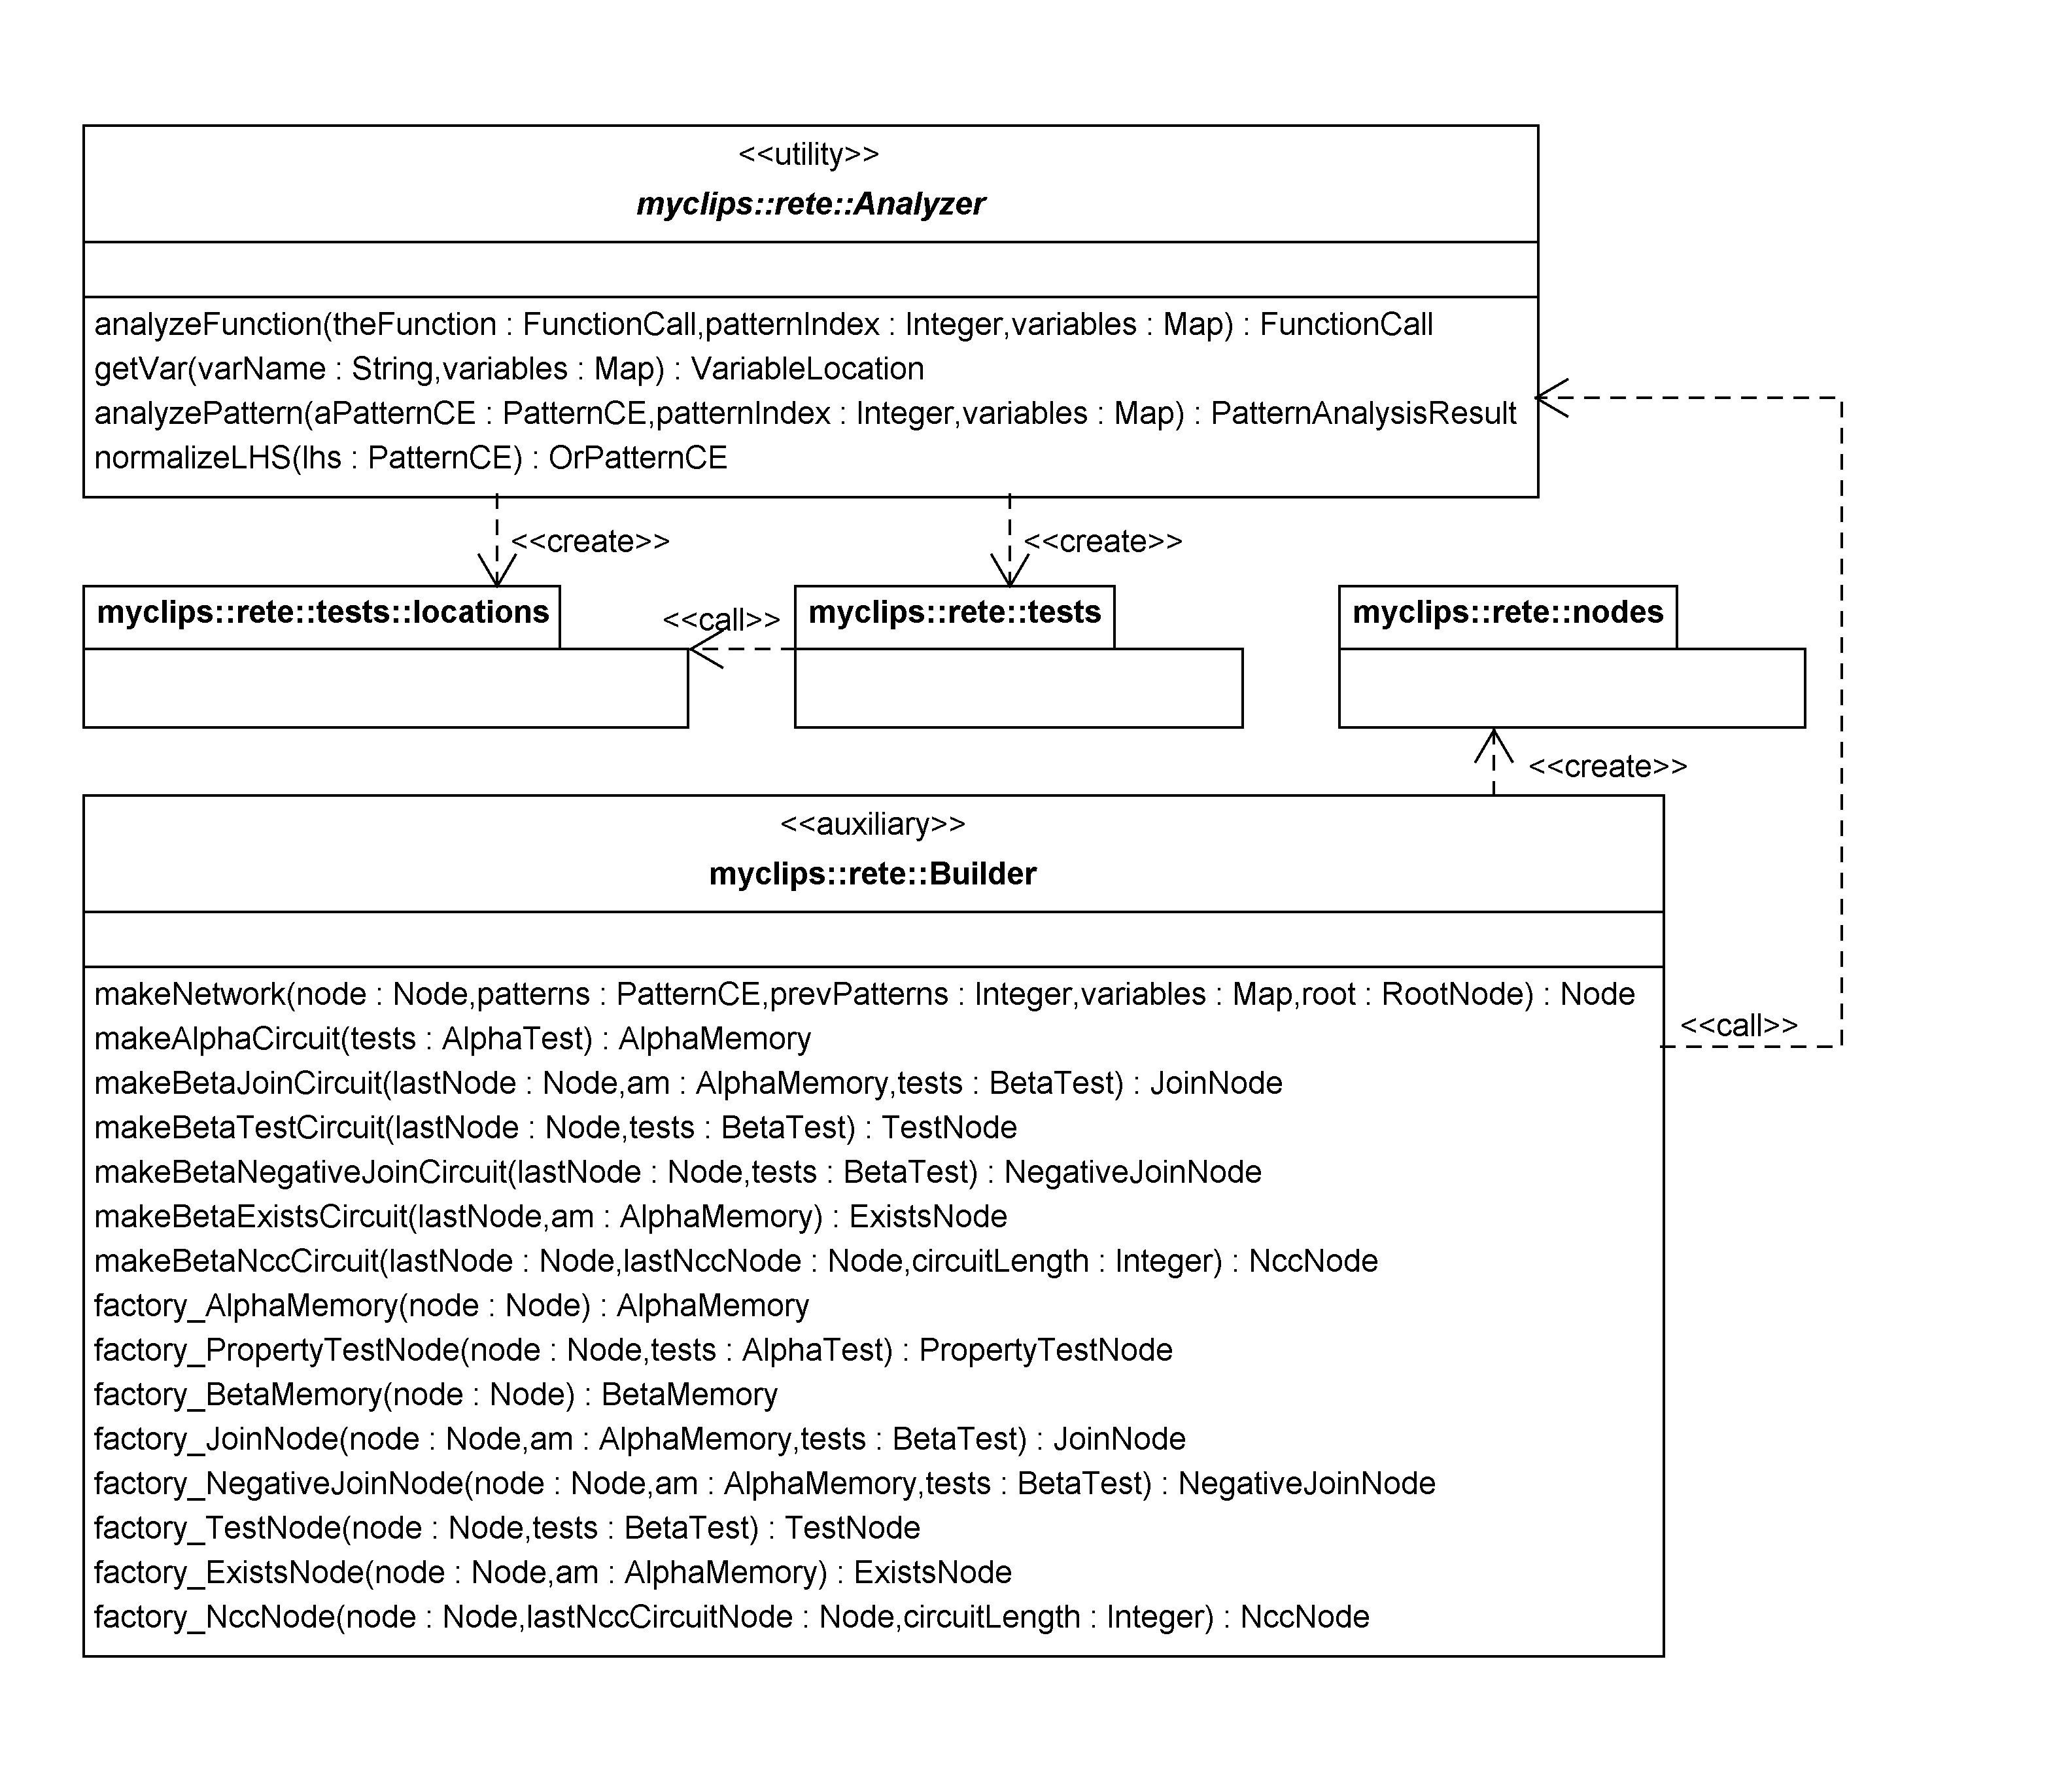
\includegraphics[width=0.9\textwidth]{Immagini/Capitolo3/Classi/myclips_rete_Builders.png}
\caption{Package \emph{myclips.rete}: vista delle classi utility per la conversione delle regole in strutture di RETE}\label{fig:class-myclips-rete-builders}
\end{figure}

Il modulo si basa sull'utilizzo di un'implementazione interpretata dell'algoritmo RETE. Attraverso l'uso di due classi utility~(\figurename~\ref{fig:class-myclips-rete-builders}), per l'analisi dei \emph{pattern} delle regole e per la costruzione del grafo, il \emph{rules-set} viene convertito nel grafo esplicito di valutazione caratteristico dell'algoritmo RETE.

La classe \emph{Analyzer} viene utilizzata per manipolare la forma dei pattern delle regole nel \emph{rules-set}, adattandole alla topologia del grafo di RETE, e individuare l'insieme dei test \emph{alpha} e \emph{beta} per i pattern, inizializzando le relative istanze delle classi di test organizzate nel package \emph{myclips.rete.tests}.

La classe \emph{Builder} ha invece il compito di creare l'insieme di nodi necessari alla costituzione del grafo, associandoli dove necessario ai test ottenuti dall'\emph{Analyzer}.
L'utilizzo dei metodi \emph{factory} per i nodi, come alternativa a normali costruttori, permette di utilizzare istanze condivise dei nodi quando possibile.

\paragraph{Compilazione delle regole}

L'algoritmo utilizzato per la compilazione delle regole segue quanto proposto in \cite{Doorenbos95productionmatching}, con alcune modifiche per permette l'utilizzo di pattern non previsti in origine come \emph{or-CE}, \emph{exists-CE} e \emph{test-CE}.

La procedura principale di compilazione ha inizio all'interno del metodo \emph{Network::addRule}: utilizzando \emph{Analyzer}, l'insieme dei pattern della regola vengono trasformati in modo che l'insieme di condizioni sia presentato in una forma normalizzata dove il primo pattern sia un elemento \emph{or-CE} con al suo interno almeno un elemento \emph{and-CE} che racchiuda le condizioni originali. Durante la normalizzazione, l'eventuale presenza di condizioni \emph{or} poste all'interno dei pattern viene trasferita nella radice della nuova \emph{LHS} normalizzata.



\begin{algorithm}
\caption{Compilazione di una regola}\label{alg:builder-makeNetwork}
\begin{algorithmic}
\Function{Builder.makeNetwork}{parent: node, conds: \textbf{list} of conditions, prevConds: integer}
\State \textbf{siano} $c_1,\dots,c_k$ le componenti di conds
\For{$i = 1 \to k$}
	\If {$c_i$ is-a Pattern-CE}
	    \State $tests_\alpha\gets$ Analysis.analyzePattern($c_i$, $\alpha$)
	    \State $memory_\alpha\gets$ Builder.makeAlphaCircuit($tests_\alpha$)
	    \State $tests_\beta\gets$ Analysis.analyzePattern($c_i$, $\beta$)
	    \State $parent\gets$ Builder.makeJoinCircuit($parent$, $memory_\alpha$, $tests_\beta$)
	\ElsIf {$c_i$ is-a Not-CE}
	    \State $tests_\alpha\gets$ Analysis.analyzePattern($c_i$, $\alpha$)
	    \State $memory_\alpha\gets$ Builder.makeAlphaCircuit($tests_\alpha$)
	    \State $tests_\beta\gets$ Analysis.analyzePattern($c_i$, $\beta$)
	    \State $parent\gets$ Builder.makeNegativeJoinCircuit($parent$, $memory_\alpha$, $tests_\beta$)
	\ElsIf {$c_i$ is-a Ncc-CE}
		\State \textbf{siano} $ncc_i$ le componenti negate da $c_i$
		\State \textbf{sia} $l$ il numero di componenti in $ncc_i$
	    \State $lastNccNode\gets$ Builder.makeNetwork($parent$, $ncc_i$, $prevConds$)
	    \State $node\gets$ Builder.makeNccCircuit($parent$, $lastNccNode$, $l$)
	\ElsIf {$c_i$ is-a Test-CE}
		\State $tests_\theta\gets$ Analysis.analyzePattern($c_i$, $\theta$)
		\State $parent\gets$ Builder.makeTestCircuit($parent$, $tests_\theta$)	
	\ElsIf {$c_i$ is-a Exists-CE}
	    \State $tests_\alpha\gets$ Analysis.analyzePattern($c_i$, $\alpha$)
	    \State $memory_\alpha\gets$ Builder.makeAlphaCircuit($tests_\alpha$)
	    \State $tests_\beta\gets$ Analysis.analyzePattern($c_i$, $\beta$)
	    \State $parent\gets$ Builder.makeExistsCircuit($parent$, $memory_\alpha$, $tests_\beta$)
	\EndIf
	\State $prevConds\gets prevConds + 1$
\EndFor
\State \Return{$node$}
\EndFunction
\end{algorithmic}
\end{algorithm}



Ogni gruppo di condizioni \emph{and-CE} genera un nuovo circuito indipendente. La compilazione del circuito ha luogo all'interno del metodo \emph{Builder::makeNetwork}~(Algoritmo~\ref{alg:builder-makeNetwork}): viene verificato il tipo di ogni pattern e quindi avviata la procedura di compilazione più indicata per lo stesso.



\begin{algorithm}
\caption{Creazione di un circuito $\alpha$}\label{alg:builder-makeAlpha}
\begin{algorithmic}
\Function{Builder.makeAlphaCircuit}{$tests_\alpha$: \textbf{list} of test}
\State \textbf{siano} $t_1,\dots,t_k$ le componenti di $tests_\alpha$
\State \textbf{sia} $root$ il nodo radice del grafo di RETE
\State $lastNode\gets root$
\For{$i = 1 \to k$}
	\State $lastNode\gets$ Builder.factory\_PropertyTestNode($lastNode$, $t_i$)
\EndFor
\State $lastNode\gets$ Builder.factory\_AlphaMemory($lastNode$)
\State \Return{$lastNode$}
\EndFunction
\end{algorithmic}
\end{algorithm}



\begin{algorithm}
\caption{Creazione di un circuito $\beta$ per il Join}\label{alg:builder-makeJoin}
\begin{algorithmic}
\Function{Builder.makeBetaJoinCircuit}{parent: node, $memory_\alpha$: node, $tests_\beta$: \textbf{list} of test}
\State $parent\gets$ Builder.factory\_BetaMemory($parent$)
\State $parent\gets$ Builder.factory\_JoinNode($parent$, $memory_\alpha$, $tests_\beta$)
\State \Return{$parent$}
\EndFunction
\end{algorithmic}
\end{algorithm}




Ad ogni tipo di pattern corrisponde una procedura apposita. Nel caso più comune, un normale \emph{Pattern-CE}, questo viene prima analizzato per l'identificazione dei test \emph{alpha} e \emph{beta}: i primi vengono utilizzati per la generazione di un circuito che filtri gli elementi della \emph{working-memory} in base ai criteri del pattern~(Algoritmo~\ref{alg:builder-makeAlpha}), mentre quelli \emph{beta} per la creazione di un nodo \emph{Join} che riunisca il circuito \emph{alpha} appena creato con le porzioni \emph{beta} della regola create in precedenza~(Algoritmo~\ref{alg:builder-makeJoin}).


\begin{algorithm}
\caption{Esempio di metodo \emph{factory} per i nodi}\label{alg:builder-factory}
\begin{algorithmic}
\Function{Builder.factory}{nodeType: un tipo di nodo, parent: node, params: \textbf{list} of parametri di creazione del nodo}
\State \textbf{siano} $child_1,\dots,child_k$ i nodi successori di $parent$
\For{$i = 1 \to k$}
	\State \textbf{siano} $params_{child_i}$ i parametri di creazioni usati per il nodo $child_i$
	\If {$child_i$ is-a $nodeType$ $\wedge$ $params = params_{child_i}$}
		\State \Return{$child_i$}
	\EndIf
\EndFor
\State \textbf{sia} $newNode$ un nuovo nodo di tipo $nodeType$ creato con i parametri $params$
\State aggiungi $newNode$ fra i successori di $parent$
\State imposta $parent$ come padre di $newNode$
\State \Return{$newNode$}
\EndFunction
\end{algorithmic}
\end{algorithm}


La procedura di generazione dei nodi~(Algoritmo~\ref{alg:builder-factory}) controlla prima la possibilità di condividere un nodo già esistente che verifichi condizioni analoghe a quelle desiderate, quindi provvede alla creazione di una nuova istanza nel caso la condivisione non sia possibile. La possibilità di condividere un nodo precedentemente creato dipende sia dall'esistenza di un nodo di tipo analogo a quello desiderato, sia dall'effettiva corrispondenza fra i test eseguiti dal nodo esistente con quelli che si desidera eseguiti dal nuovo nodo.

Di seguito sono mostrati gli algoritmi per la generazione delle varie tipologie di circuito


\begin{algorithm}[h]
\caption{Creazione di un circuito $\beta$ per il NegativeJoin}\label{alg:builder-makeNegativeJoin}
\begin{algorithmic}
\Function{Builder.makeNegativeJoinCircuit}{parent: node, $memory_\alpha$: node, $tests_\beta$: \textbf{list} of test}
\State $parent\gets$ Builder.factory\_NegativeJoinNode($parent$, $memory_\alpha$, $tests_\beta$)
\State \Return{$parent$}
\EndFunction
\end{algorithmic}
\end{algorithm}




\begin{algorithm}[h]
\caption{Creazione di un circuito $\beta$ per Exists}\label{alg:builder-makeExists}
\begin{algorithmic}
\Function{Builder.makeBetaExistsCircuit}{parent: node, $memory_\alpha$: node}
\State $parent\gets$ Builder.factory\_BetaMemory($parent$)
\State $parent\gets$ Builder.factory\_ExistsNode($parent$, $memory_\alpha$)
\State \Return{$parent$}
\EndFunction
\end{algorithmic}
\end{algorithm}




\begin{algorithm}
\caption{Creazione di un circuito $\beta$ per gruppi di negazioni (NCC)}\label{alg:builder-makeNcc}
\begin{algorithmic}
\Function{Builder.makeBetaNccCircuit}{parent: node, $ncc$: node, $l$: Integer}
\State $parent\gets$ Builder.factory\_NccNode($parent$, $ncc$, $l$)
\State \Return{$parent$}
\EndFunction
\end{algorithmic}
\end{algorithm}




\begin{algorithm}
\caption{Creazione di un circuito $\beta$ per il Test}\label{alg:builder-makeTest}
\begin{algorithmic}
\Function{Builder.makeBetaTestCircuit}{parent: node, $memory_\alpha$: node, $tests_\theta$: \textbf{list} of test}
\State $parent\gets$ Builder.factory\_BetaMemory($parent$)
\State $parent\gets$ Builder.factory\_TestNode($parent$, $memory_\alpha$, $tests_\theta$)
\State \Return{$parent$}
\EndFunction
\end{algorithmic}
\end{algorithm}




\begin{algorithm}
\caption{Algoritmo di generazione dei test $\alpha$}\label{alg:analyzer-test-alpha}
\begin{algorithmic}
\Function{Analyzer.analyzePatternAlpha}{$c$: pattern, $pi$: Integer}
\State \textbf{sia} $tests$ un vettore di test $\alpha$ inizialmente vuoto
\State \textbf{siano} $p_i$ le proprietà definite dal pattern $c$
\For{$i = 1 \to k$}
	\If {$p_i$ $\neg$ is-a $Variabile$}
		\State $t \gets$ un test adatto a descrivere $p_i$
		\State accoda $t$ a $tests$
	\EndIf
\EndFor
\State \Return{$tests$}
\EndFunction
\end{algorithmic}
\end{algorithm}



\begin{algorithm}
\caption{Algoritmo di generazione dei test $\beta$}\label{alg:analyzer-test-beta}
\begin{algorithmic}
\Function{Analyzer.analyzePatternBeta}{$c$: pattern, $pi$: integer}
\State \textbf{sia} $tests$ un vettore di test $\beta$ inizialmente vuoto
\State \textbf{sia} $vars$ un insieme di variabili identificate nel pattern inizialmente vuoto
\State \textbf{siano} $p_i$ le proprietà definite dal pattern $c$
\For{$i = 1 \to k$}
	\If {$p_i$ is-a $Variabile$}
		\If {$p_i$ e' gia contenuto in $vars$}
			\State $prev_{p_i}\gets$ recupera le coordinate della precedente posizione di $p_i$ da $vars$
			\State $t \gets$ un test adatto a verificare che il valore associato alla posizione $prev_{p_i}$ sia uguale a quella di $p_i$
			\State accoda $t$ a $tests$
		\Else
			\State $t \gets$ un test adatto a descrivere $p_i$
			\State inserisci le coordinate di $p_i$ all'interno di $vars$
		\EndIf
	\EndIf
\EndFor
\State \Return{$tests$}
\EndFunction
\end{algorithmic}
\end{algorithm}


%
\begin{algorithm}
\caption{Esempio di metodo \emph{factory} per i nodi}\label{alg:builder-factory}
\begin{algorithmic}
\Function{Builder.factory}{nodeType: un tipo di nodo, parent: node, params: \textbf{list} of parametri di creazione del nodo}
\State \textbf{siano} $child_1,\dots,child_k$ i nodi successori di $parent$
\For{$i = 1 \to k$}
	\State \textbf{siano} $params_{child_i}$ i parametri di creazioni usati per il nodo $child_i$
	\If {$child_i$ is-a $nodeType$ $\wedge$ $params = params_{child_i}$}
		\State \Return{$child_i$}
	\EndIf
\EndFor
\State \textbf{sia} $newNode$ un nuovo nodo di tipo $nodeType$ creato con i parametri $params$
\State aggiungi $newNode$ fra i successori di $parent$
\State imposta $parent$ come padre di $newNode$
\State \Return{$newNode$}
\EndFunction
\end{algorithmic}
\end{algorithm}



\begin{algorithm}
\caption{Metodo \emph{factory} per i \emph{PropertyTestNode}}\label{alg:builder-factory-property}
\begin{algorithmic}
\Function{Builder.factoryPropertyTestNode}{parent: node, t: un test di tipo $\alpha$}
\State \textbf{siano} $child_1,\dots,child_k$ i nodi successori di $parent$
\For{$i = 1 \to k$}
	\If {$child_i$ is-a $PropertyTestNode$ $\wedge$ il test di $child_i = t$}
		\State \Return{$child_i$}
	\EndIf
\EndFor
\State \textbf{sia} $newNode$ un nuovo nodo di tipo $PropertyTestNode$ creato con il test $t$
\State aggiungi $newNode$ fra i successori di $parent$
\State imposta $parent$ come padre di $newNode$
\State \Return{$newNode$}
\EndFunction
\end{algorithmic}
\end{algorithm}


%
\begin{algorithm}
\caption{Esempio di metodo \emph{factory} per i nodi}\label{alg:builder-factory}
\begin{algorithmic}
\Function{Builder.factory}{nodeType: un tipo di nodo, parent: node, params: \textbf{list} of parametri di creazione del nodo}
\State \textbf{siano} $child_1,\dots,child_k$ i nodi successori di $parent$
\For{$i = 1 \to k$}
	\State \textbf{siano} $params_{child_i}$ i parametri di creazioni usati per il nodo $child_i$
	\If {$child_i$ is-a $nodeType$ $\wedge$ $params = params_{child_i}$}
		\State \Return{$child_i$}
	\EndIf
\EndFor
\State \textbf{sia} $newNode$ un nuovo nodo di tipo $nodeType$ creato con i parametri $params$
\State aggiungi $newNode$ fra i successori di $parent$
\State imposta $parent$ come padre di $newNode$
\State \Return{$newNode$}
\EndFunction
\end{algorithmic}
\end{algorithm}


%
\begin{algorithm}
\caption{Esempio di metodo \emph{factory} per i nodi}\label{alg:builder-factory}
\begin{algorithmic}
\Function{Builder.factory}{nodeType: un tipo di nodo, parent: node, params: \textbf{list} of parametri di creazione del nodo}
\State \textbf{siano} $child_1,\dots,child_k$ i nodi successori di $parent$
\For{$i = 1 \to k$}
	\State \textbf{siano} $params_{child_i}$ i parametri di creazioni usati per il nodo $child_i$
	\If {$child_i$ is-a $nodeType$ $\wedge$ $params = params_{child_i}$}
		\State \Return{$child_i$}
	\EndIf
\EndFor
\State \textbf{sia} $newNode$ un nuovo nodo di tipo $nodeType$ creato con i parametri $params$
\State aggiungi $newNode$ fra i successori di $parent$
\State imposta $parent$ come padre di $newNode$
\State \Return{$newNode$}
\EndFunction
\end{algorithmic}
\end{algorithm}


%
\begin{algorithm}
\caption{Esempio di metodo \emph{factory} per i nodi}\label{alg:builder-factory}
\begin{algorithmic}
\Function{Builder.factory}{nodeType: un tipo di nodo, parent: node, params: \textbf{list} of parametri di creazione del nodo}
\State \textbf{siano} $child_1,\dots,child_k$ i nodi successori di $parent$
\For{$i = 1 \to k$}
	\State \textbf{siano} $params_{child_i}$ i parametri di creazioni usati per il nodo $child_i$
	\If {$child_i$ is-a $nodeType$ $\wedge$ $params = params_{child_i}$}
		\State \Return{$child_i$}
	\EndIf
\EndFor
\State \textbf{sia} $newNode$ un nuovo nodo di tipo $nodeType$ creato con i parametri $params$
\State aggiungi $newNode$ fra i successori di $parent$
\State imposta $parent$ come padre di $newNode$
\State \Return{$newNode$}
\EndFunction
\end{algorithmic}
\end{algorithm}


%
\begin{algorithm}
\caption{Esempio di metodo \emph{factory} per i nodi}\label{alg:builder-factory}
\begin{algorithmic}
\Function{Builder.factory}{nodeType: un tipo di nodo, parent: node, params: \textbf{list} of parametri di creazione del nodo}
\State \textbf{siano} $child_1,\dots,child_k$ i nodi successori di $parent$
\For{$i = 1 \to k$}
	\State \textbf{siano} $params_{child_i}$ i parametri di creazioni usati per il nodo $child_i$
	\If {$child_i$ is-a $nodeType$ $\wedge$ $params = params_{child_i}$}
		\State \Return{$child_i$}
	\EndIf
\EndFor
\State \textbf{sia} $newNode$ un nuovo nodo di tipo $nodeType$ creato con i parametri $params$
\State aggiungi $newNode$ fra i successori di $parent$
\State imposta $parent$ come padre di $newNode$
\State \Return{$newNode$}
\EndFunction
\end{algorithmic}
\end{algorithm}


%
\begin{algorithm}
\caption{Esempio di metodo \emph{factory} per i nodi}\label{alg:builder-factory}
\begin{algorithmic}
\Function{Builder.factory}{nodeType: un tipo di nodo, parent: node, params: \textbf{list} of parametri di creazione del nodo}
\State \textbf{siano} $child_1,\dots,child_k$ i nodi successori di $parent$
\For{$i = 1 \to k$}
	\State \textbf{siano} $params_{child_i}$ i parametri di creazioni usati per il nodo $child_i$
	\If {$child_i$ is-a $nodeType$ $\wedge$ $params = params_{child_i}$}
		\State \Return{$child_i$}
	\EndIf
\EndFor
\State \textbf{sia} $newNode$ un nuovo nodo di tipo $nodeType$ creato con i parametri $params$
\State aggiungi $newNode$ fra i successori di $parent$
\State imposta $parent$ come padre di $newNode$
\State \Return{$newNode$}
\EndFunction
\end{algorithmic}
\end{algorithm}


%
\begin{algorithm}
\caption{Esempio di metodo \emph{factory} per i nodi}\label{alg:builder-factory}
\begin{algorithmic}
\Function{Builder.factory}{nodeType: un tipo di nodo, parent: node, params: \textbf{list} of parametri di creazione del nodo}
\State \textbf{siano} $child_1,\dots,child_k$ i nodi successori di $parent$
\For{$i = 1 \to k$}
	\State \textbf{siano} $params_{child_i}$ i parametri di creazioni usati per il nodo $child_i$
	\If {$child_i$ is-a $nodeType$ $\wedge$ $params = params_{child_i}$}
		\State \Return{$child_i$}
	\EndIf
\EndFor
\State \textbf{sia} $newNode$ un nuovo nodo di tipo $nodeType$ creato con i parametri $params$
\State aggiungi $newNode$ fra i successori di $parent$
\State imposta $parent$ come padre di $newNode$
\State \Return{$newNode$}
\EndFunction
\end{algorithmic}
\end{algorithm}


%
\begin{algorithm}
\caption{Esempio di metodo \emph{factory} per i nodi}\label{alg:builder-factory}
\begin{algorithmic}
\Function{Builder.factory}{nodeType: un tipo di nodo, parent: node, params: \textbf{list} of parametri di creazione del nodo}
\State \textbf{siano} $child_1,\dots,child_k$ i nodi successori di $parent$
\For{$i = 1 \to k$}
	\State \textbf{siano} $params_{child_i}$ i parametri di creazioni usati per il nodo $child_i$
	\If {$child_i$ is-a $nodeType$ $\wedge$ $params = params_{child_i}$}
		\State \Return{$child_i$}
	\EndIf
\EndFor
\State \textbf{sia} $newNode$ un nuovo nodo di tipo $nodeType$ creato con i parametri $params$
\State aggiungi $newNode$ fra i successori di $parent$
\State imposta $parent$ come padre di $newNode$
\State \Return{$newNode$}
\EndFunction
\end{algorithmic}
\end{algorithm}


\clearpage

\paragraph{Nodi del grafo di RETE}

Il set di nodi che supportano l'implementazione dell'algoritmo RETE sono realizzazioni di un set di interfacce fondamentali (\figurename~\ref{fig:class-myclips-rete-interfaces}) che hanno il compito di formalizzare i metodi usati dai nodi per lo scambio di segnali e rendere possibile l'attraversamento da parte dei \emph{Token}.

\begin{figure}
\centering
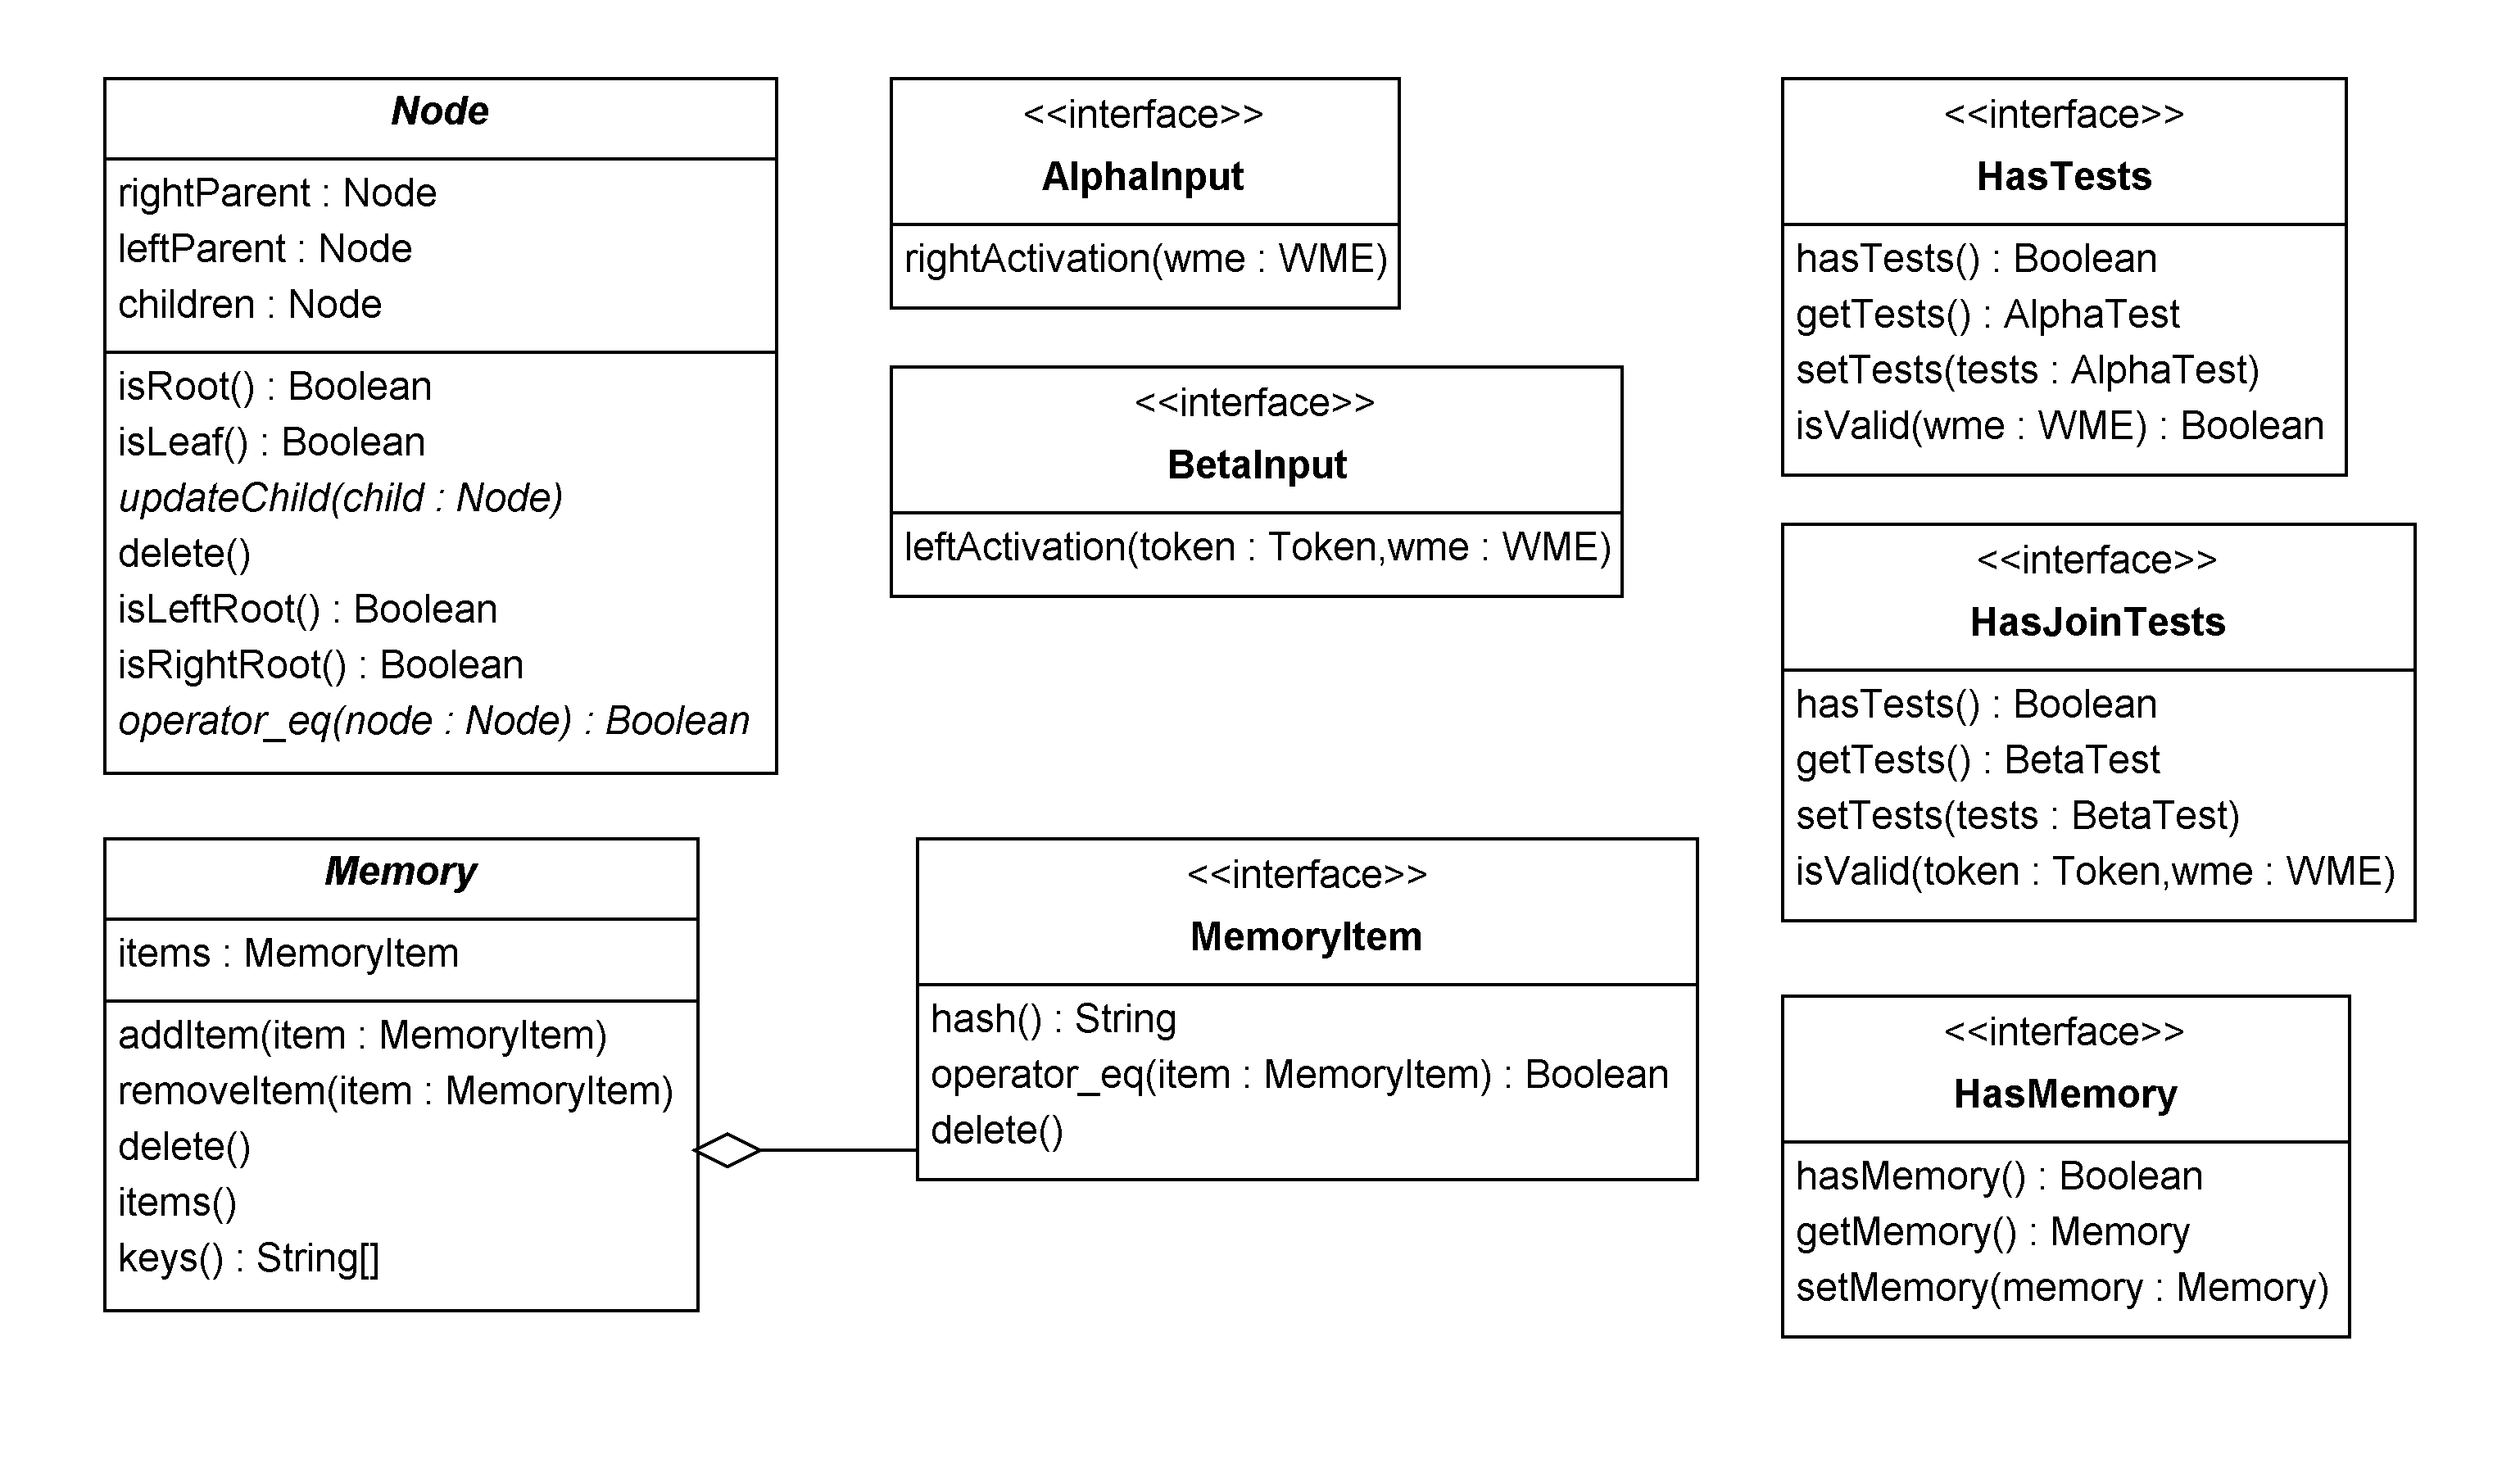
\includegraphics[width=1\textwidth]{Immagini/Capitolo3/Classi/myclips_rete_Interfacce.png}
\caption{Package \emph{myclips.rete}: vista delle interfacce di base usate dai nodi per l'implementazione di RETE}\label{fig:class-myclips-rete-interfaces}
\end{figure}

La classe astratta \emph{Node}, specializzata da tutti i nodi, rappresenta la struttura di base comune a tutti i tipi: memorizza i riferimenti ai nodi padre (destro per tutti i nodi, sinistro solo per quelli a due input) e i riferimenti ai nodi successori. Le memorie, \emph{alpha} e \emph{beta}, ed i nodi che memorizzano attivazioni parziali estendono inoltre la classe \emph{Memory}. Le ulteriori interfacce presenti in \figurename~\ref{fig:class-myclips-rete-interfaces} formalizzano i metodi relativi all'esecuzione dei test e alla propagazione delle attivazioni parziali.

\begin{figure}
\centering
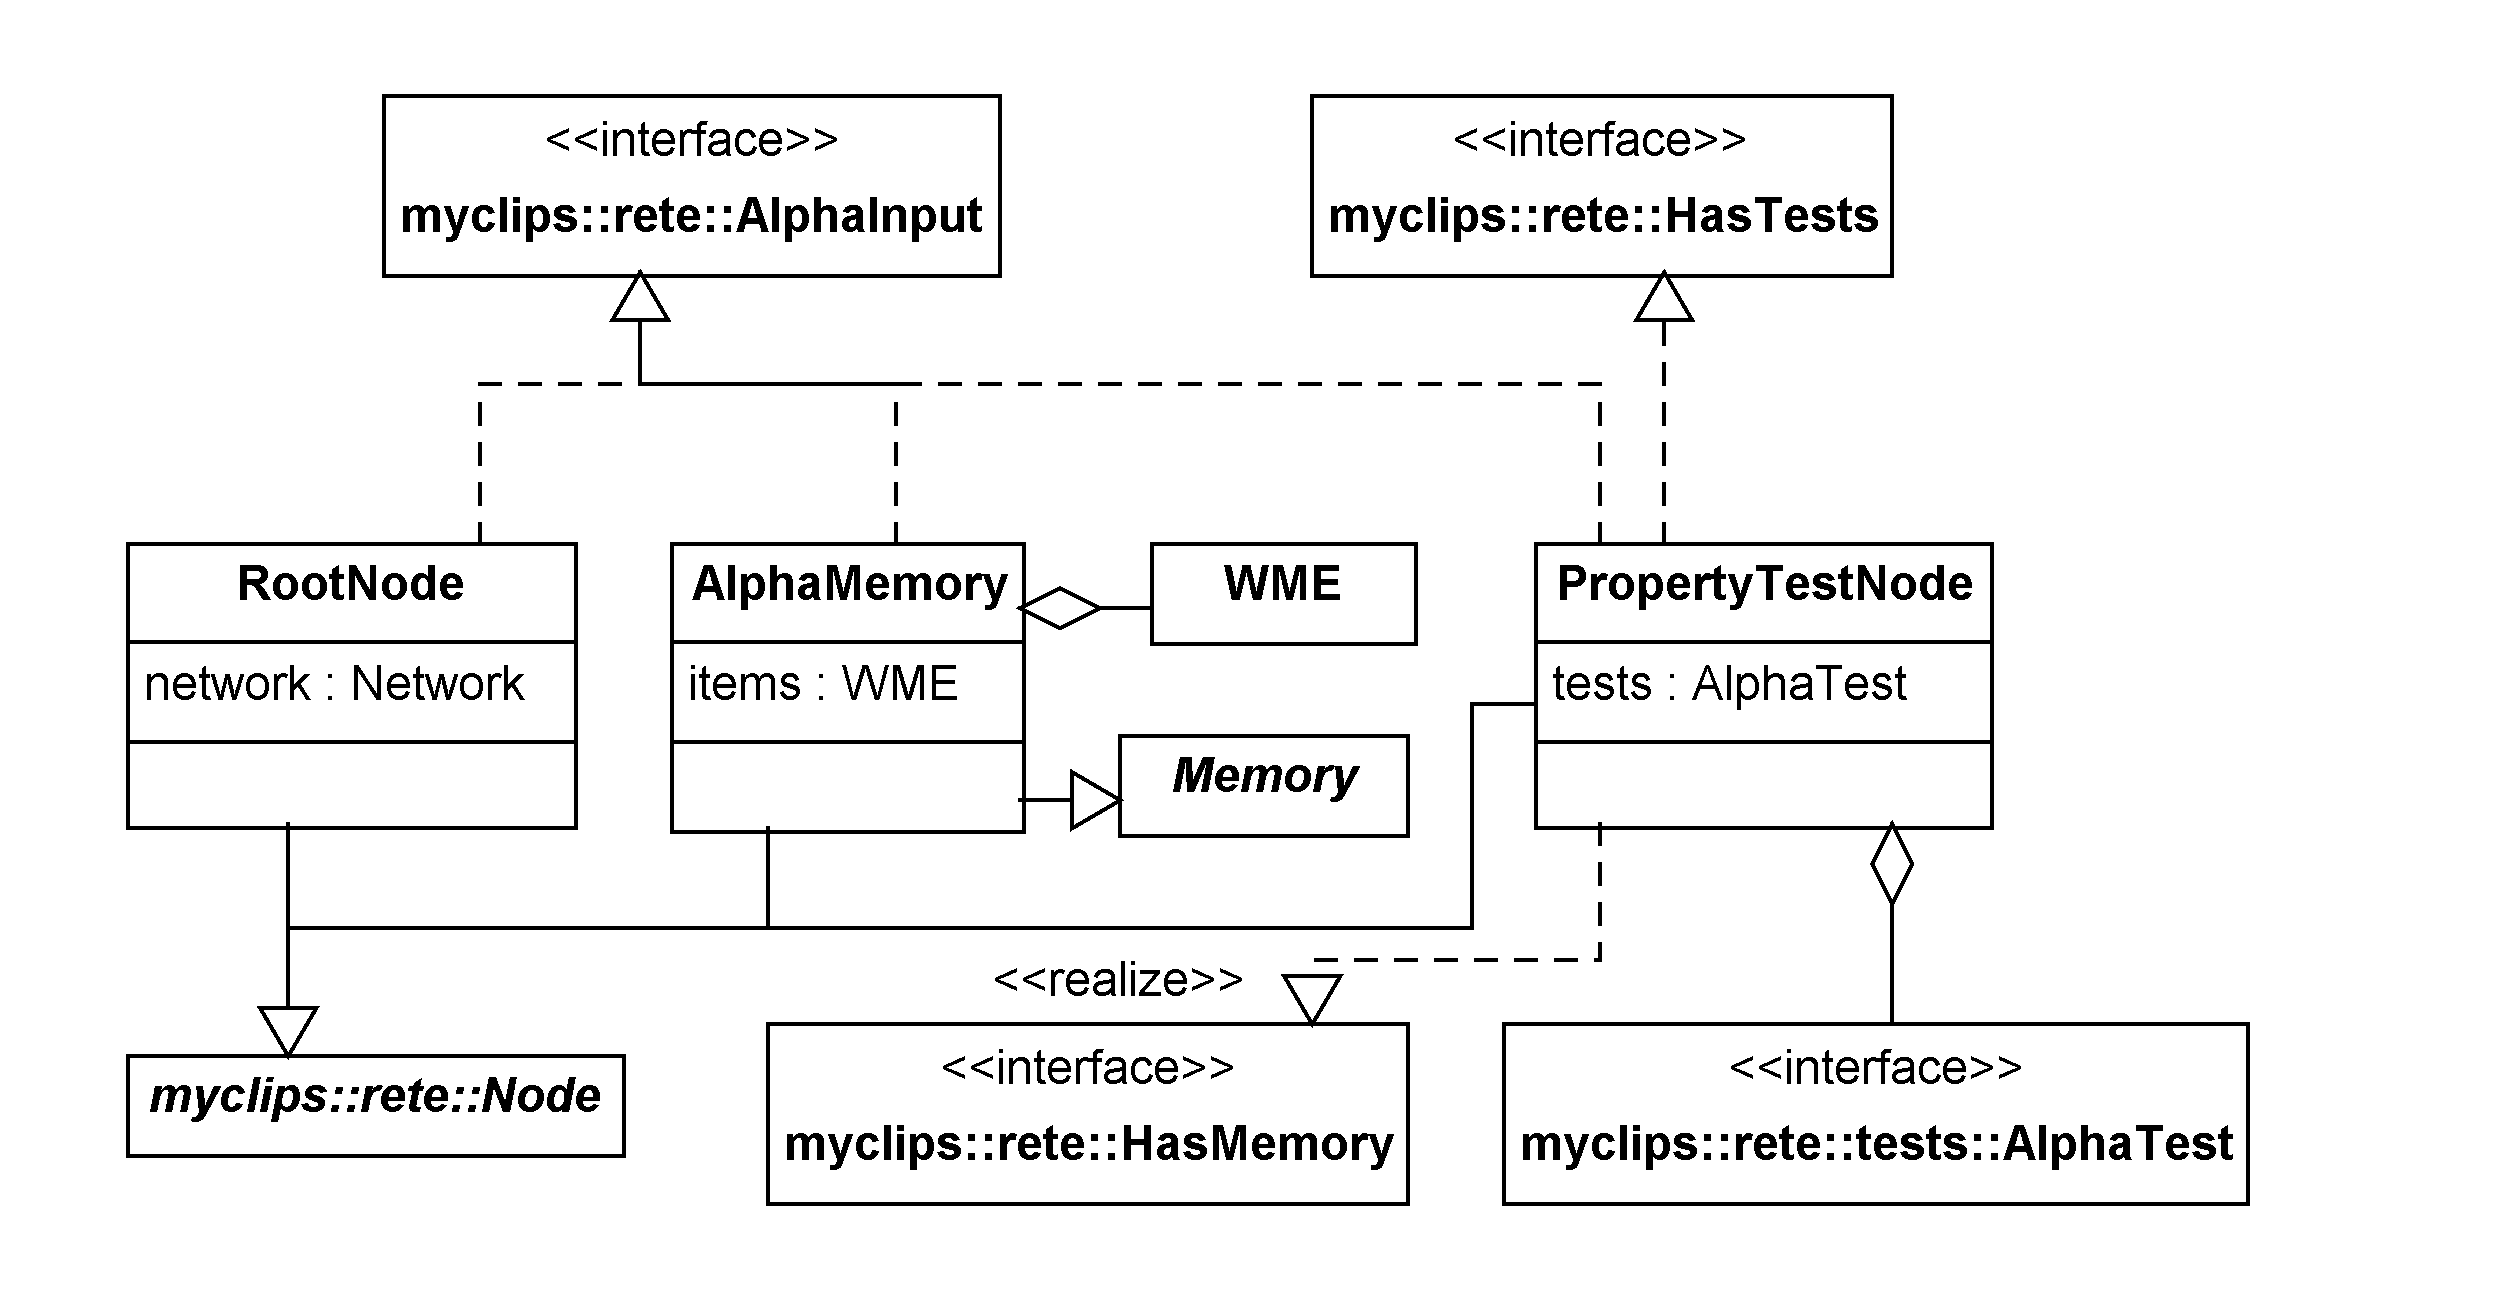
\includegraphics[width=1\textwidth]{Immagini/Capitolo3/Classi/myclips_rete_nodes_Nodi-Alpha.png}
\caption{Package \emph{myclips.rete.nodes}: vista dei nodi della pozione \emph{alpha}}\label{fig:class-myclips-rete-nodes-alpha}
\end{figure}

\begin{figure}
\centering
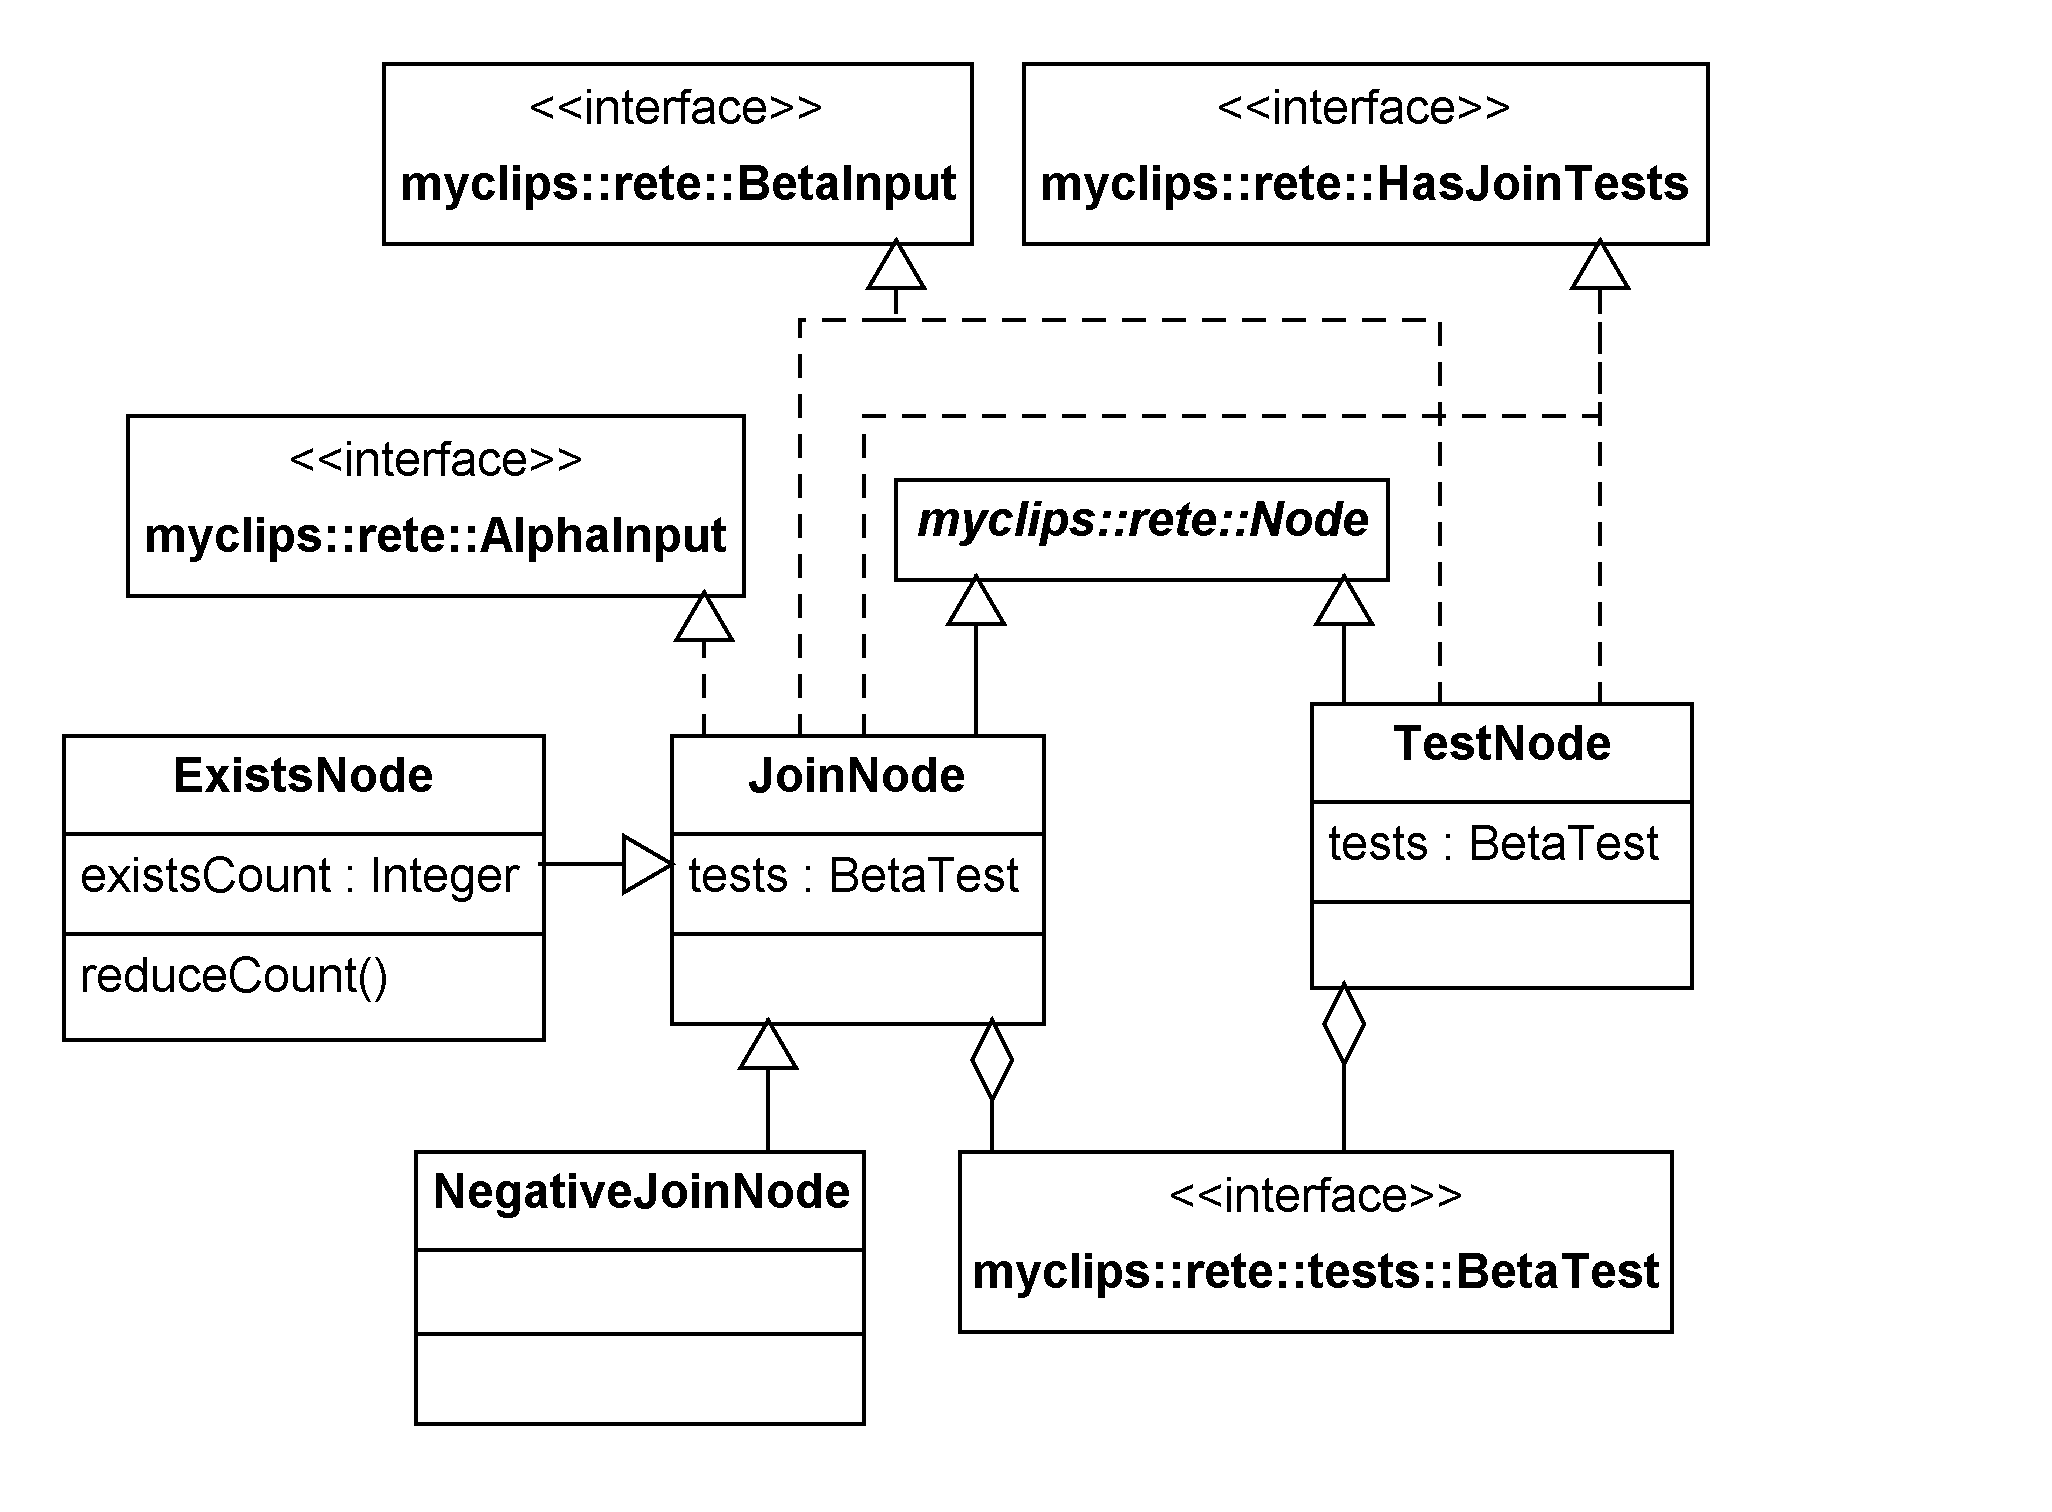
\includegraphics[width=1\textwidth]{Immagini/Capitolo3/Classi/myclips_rete_nodes_Join-Tests-Exists-Negative-Nodes.png}
\caption{Package \emph{myclips.rete.nodes}: vista dei nodi della pozione \emph{beta}}\label{fig:class-myclips-rete-nodes-beta}
\end{figure}

\begin{figure}
\centering
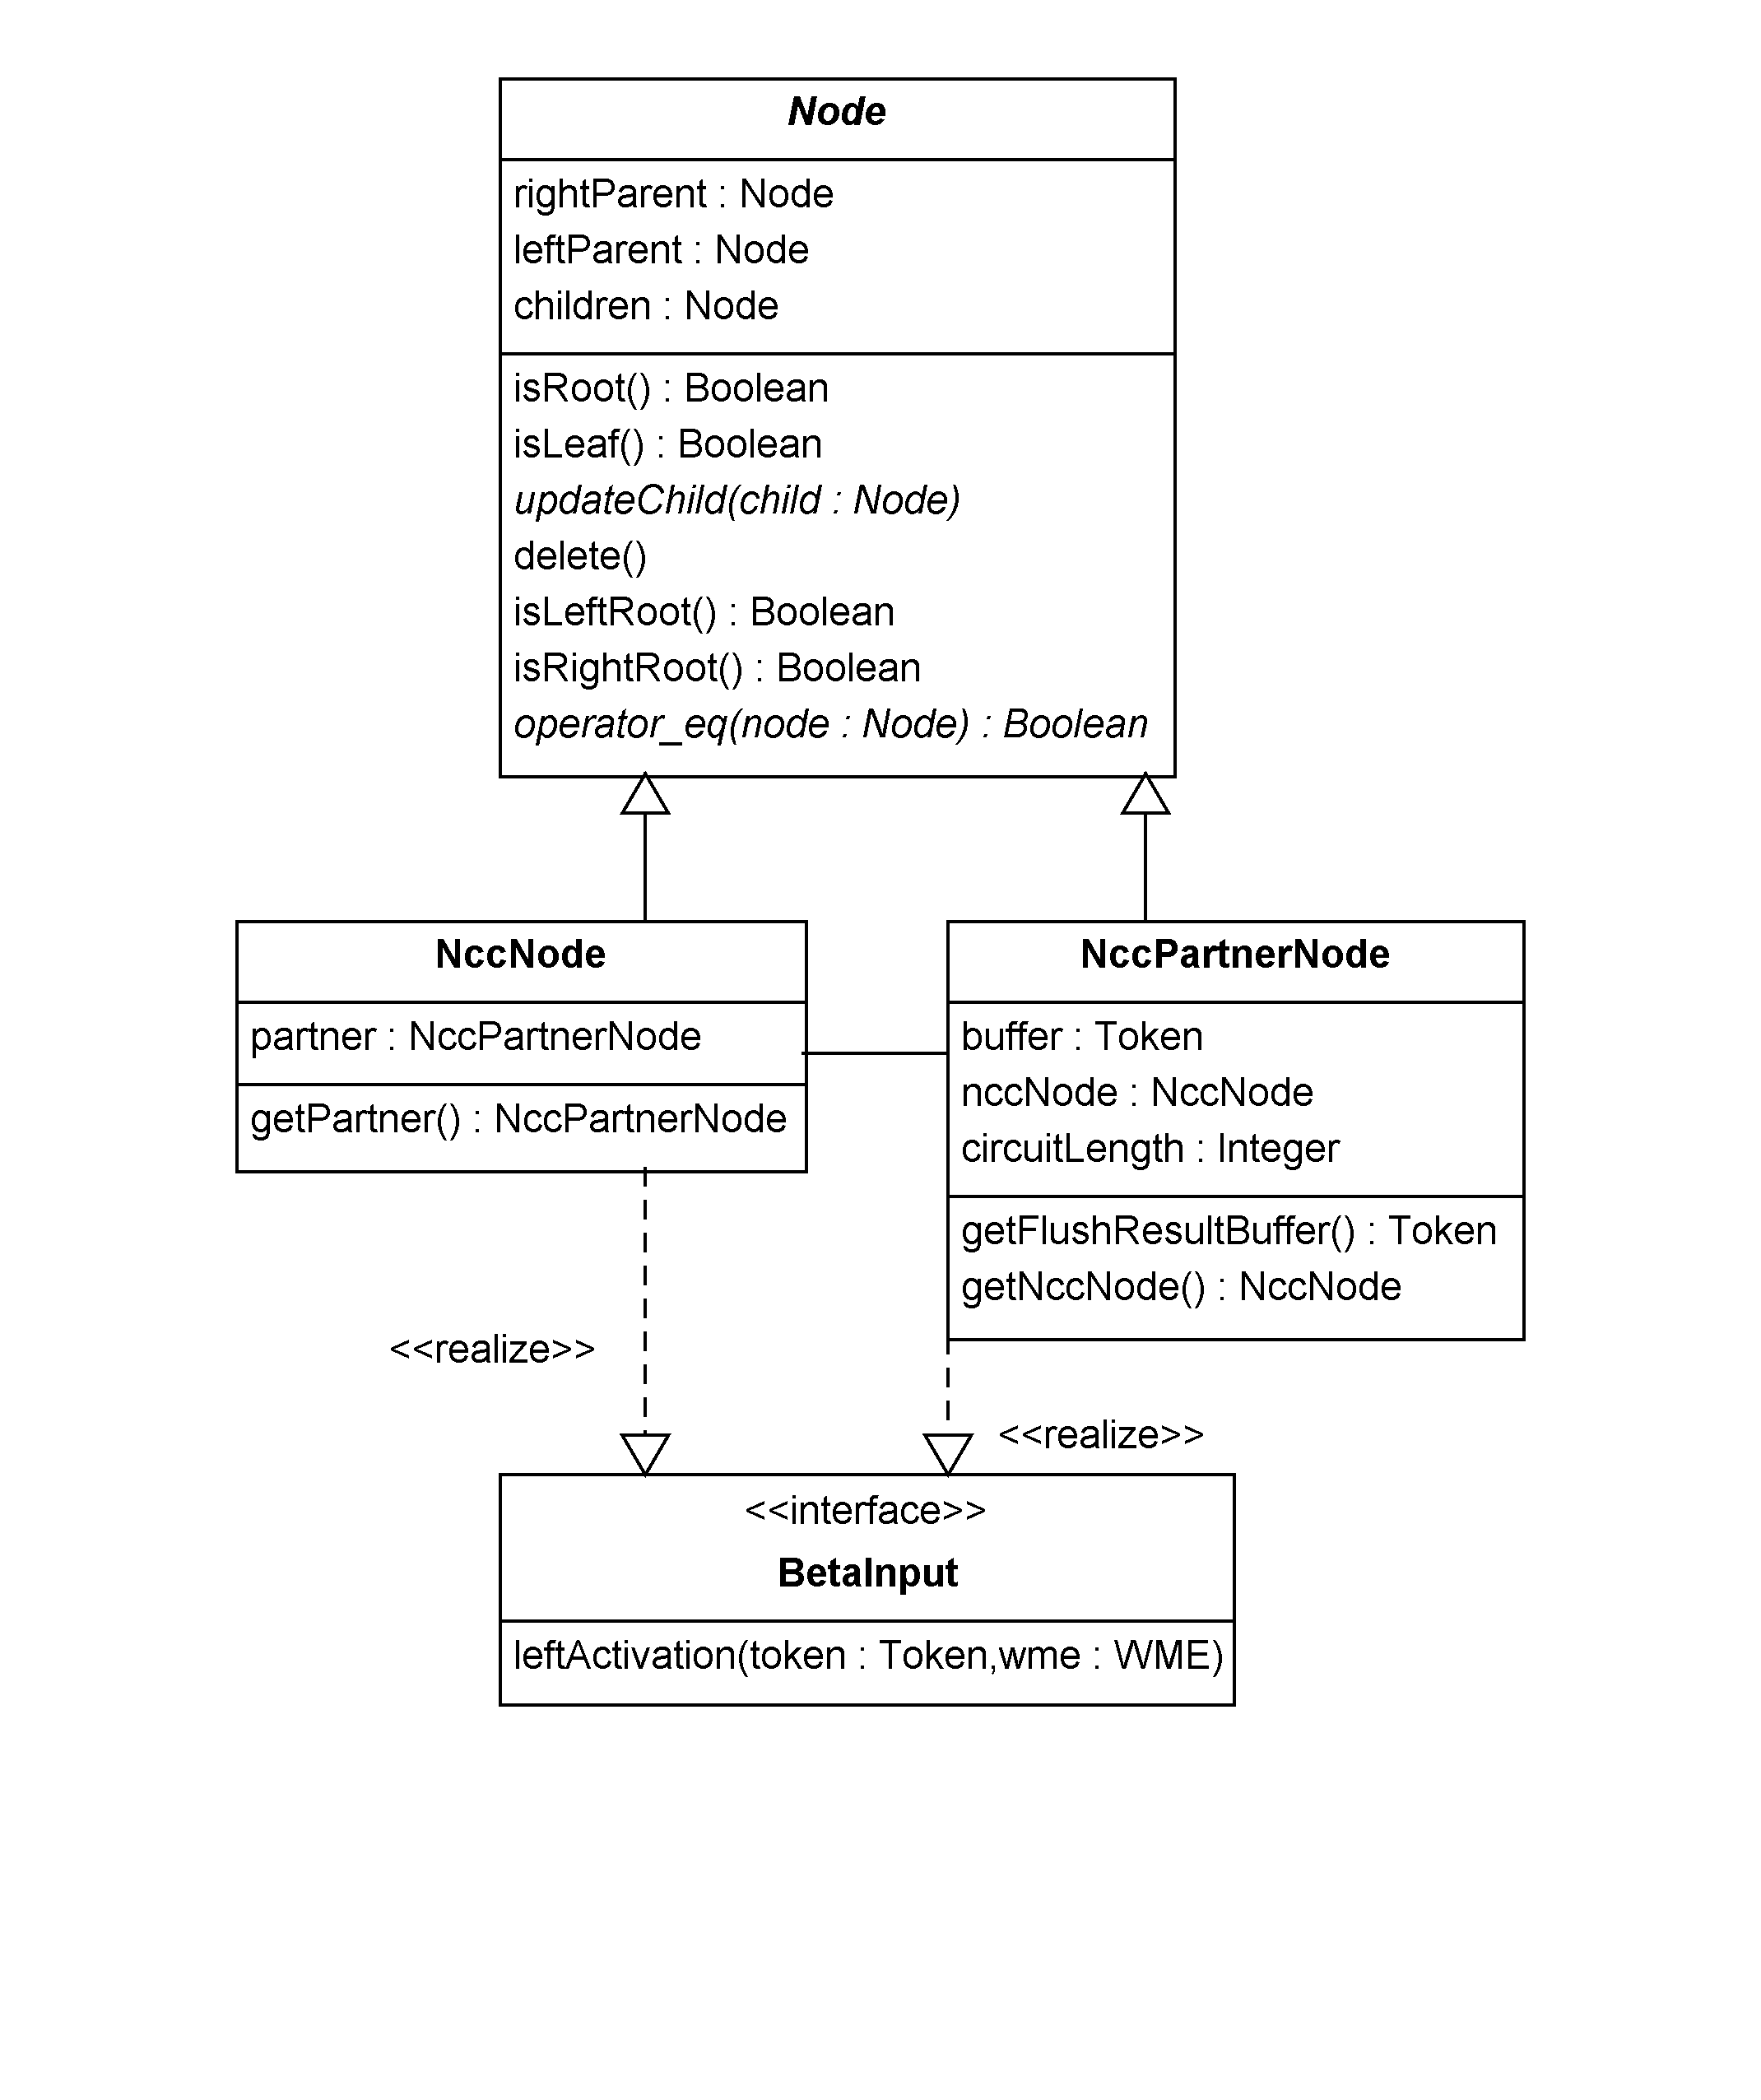
\includegraphics[width=1\textwidth]{Immagini/Capitolo3/Classi/myclips_rete_nodes_Ncc-Partner-Nodes.png}
\caption{Package \emph{myclips.rete.nodes}: vista dei nodi della pozione \emph{beta} (nodi \emph{Ncc})}\label{fig:class-myclips-rete-nodes-beta-ncc}
\end{figure}


Una classificazione approssimativa dei nodi può essere realizzata suddividendoli in base alla porzione della RETE che realizzano: \emph{alpha}~(\figurename~\ref{fig:class-myclips-rete-nodes-alpha}) o \emph{beta}~(\figurename~\ref{fig:class-myclips-rete-nodes-beta} e \ref{fig:class-myclips-rete-nodes-beta-ncc}). 

Ogni tipo di nodo svolge una specifica funzione, spesso anche in relazione alla tipologia di test che può inglobare:
\begin{description}
	\item[RootNode:] la radice del grafo radicato orientato che realizza RETE.
	
	\item[PropertyTestNode:] associabile a test di tipo \emph{alpha}, può effettuare controlli su elementi costanti di un pattern.
	
	\item[AlphaMemory:] unità locale di memoria posta a termine di ogni \emph{circuito alpha}. Conserva gli elementi \emph{WME} che hanno attraversato con successo il circuito a cui il nodo è collegato.
	
	\item[JoinNode:] nodo a due input, viene utilizzato per riunire istanze \emph{WME} provenienti dai due rami del grafo in \emph{Token} da propagare se i test collegati al nodo risultano verificati. Questo tipo di nodi viene utilizzato per realizzare i test di coerenza sul valore delle variabili presenti in pattern multipli.
	
	\item[NegativeJoinNode:] specializzazione del nodo \emph{JoinNode}, propaga un \emph{Token} solo se tutti i test di coerenza associati al nodo non risultano soddisfatti.
	
	\item[TestNode:] nodo con input singolo, esegue dei test su un \emph{Token} (spesso associati all'esecuzioni di funzioni dinamiche) e lo propaga nei casi di esito positivo.

	\item[ExistsNode:] nodo a due input utilizzato per fornire supporto al quantificatore esistenziale ($\exists$) all'interno delle porzioni LHS delle regole. Un'attivazione proveniente dal ramo sinistro (quindi \emph{beta}) del grafo viene propagato soltanto se esiste almeno un elemento all'interno dell'unità di memoria collegata come input destro (quindi \emph{alpha}).
	
	\item[NccNode] e \textbf{NccPartnerNode:} i nodi \emph{Ncc}~(\figurename~\ref{fig:class-myclips-rete-nodes-beta-ncc}) vengono utilizzati per realizzare negazioni di gruppi di condizioni. Le attivazioni provenienti dal ramo sinistro vengono propagate soltanto quando non viene identificata nessuna attivazione proveniente dal circuito negato associato.
	
\end{description} 

\paragraph{Classi di Test}

Gli algoritmi utilizzati dai nodi per eseguire le verifiche sulle attivazioni e gli elementi della \emph{working-memory} sono organizzati all'interno del \emph{package} \emph{myclips.rete.tests}. Alla base della strategia di progettazione dei test c'è l'utilizzo del \emph{design pattern} comportamentale \emph{Strategy}: allo scopo di rendere gli algoritmi di test intercambiabili fra loro, vengono fornite due interfacce di base che tutti i test realizzano. La scelta dell'interfaccia da implementare indica la classe di nodi che potranno utilizzare i test: \emph{AlphaTest} per i test utilizzabili nei nodi \emph{Alpha}, \emph{BetaTest} per quelli nei nodi \emph{Beta}.

\begin{figure}
\centering
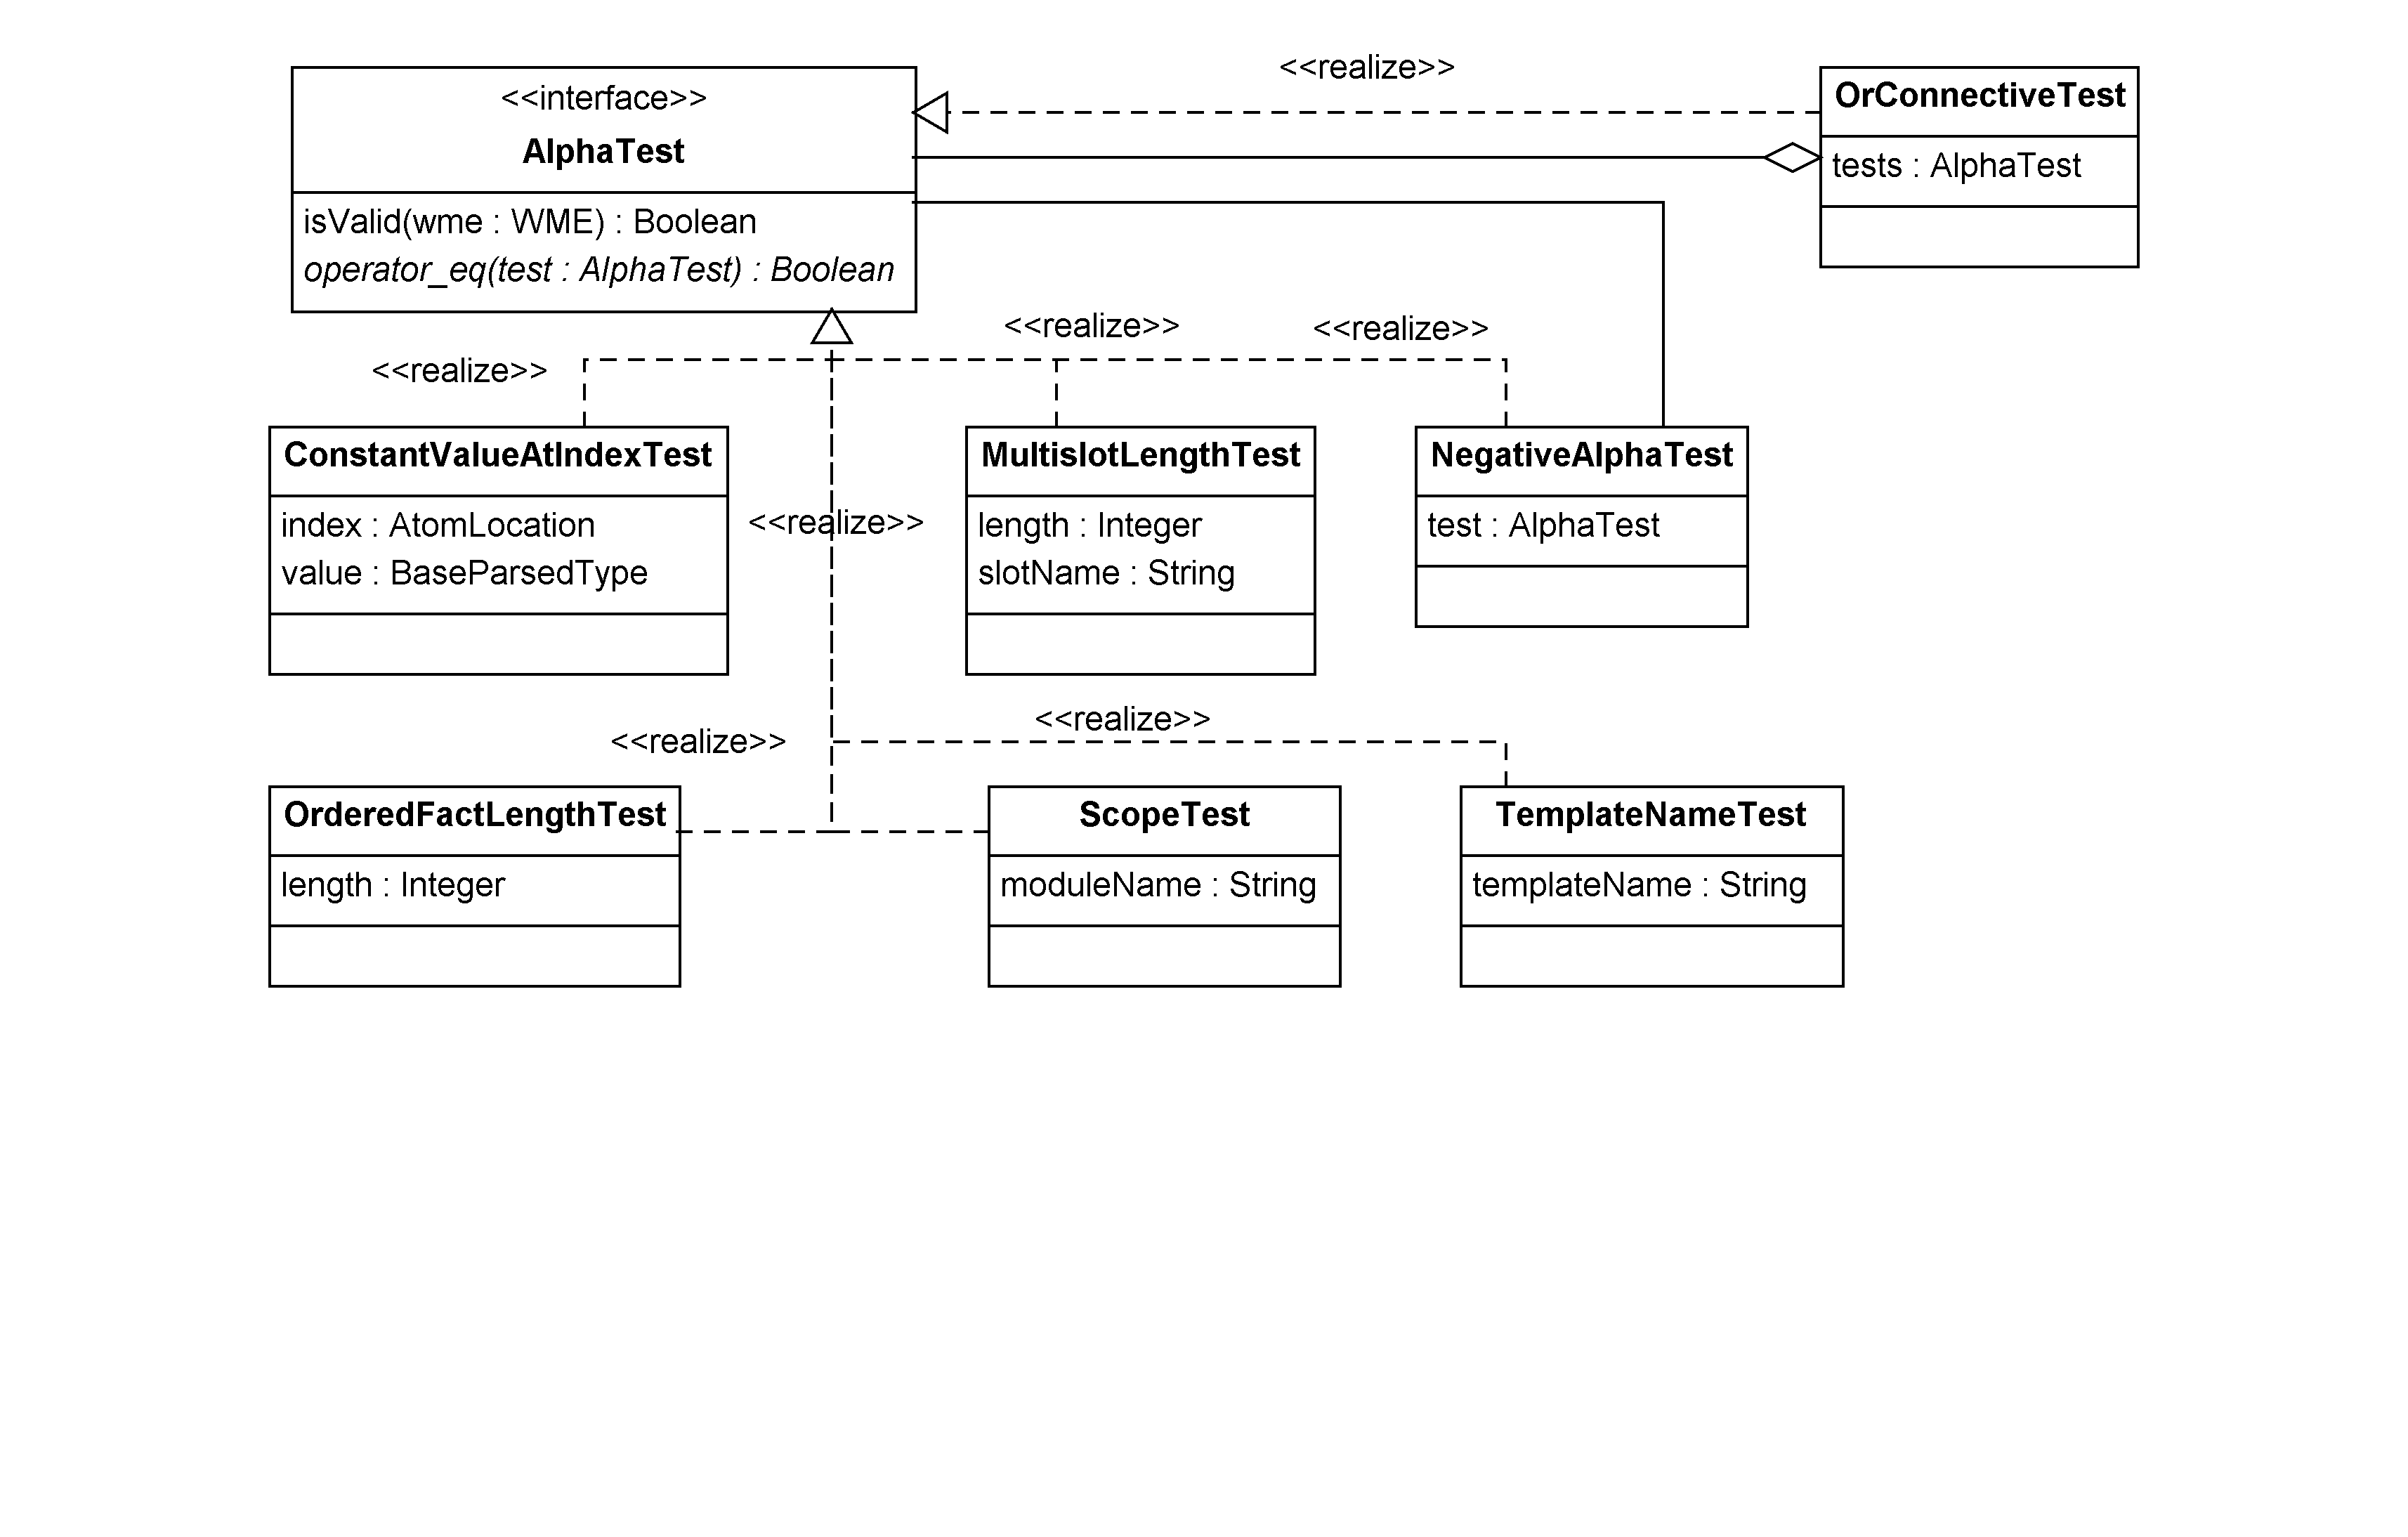
\includegraphics[width=1\textwidth]{Immagini/Capitolo3/Classi/myclips_rete_tests_Alpha.png}
\caption{Package \emph{myclips.rete.tests}: vista dei test eseguiti nella porzione \emph{alpha}}\label{fig:class-myclips-rete-tests-alpha}
\end{figure}

La prima tipologia (\figurename~\ref{fig:class-myclips-rete-tests-alpha}) esegue test su singoli elementi \emph{WME}, valutando il possibile inserimento all'interno delle memorie locali presenti al termine dei circuiti \emph{alpha}. Gli algoritmi possono valutare caratteristiche differenti dei singoli elementi come la lunghezza delle sequenze di \emph{OrderedFact}, la visibilità relativa ad un determinato \emph{Scope}, la presenza di un elemento costante in una determinata coordinata, etc.

\begin{figure}[h]
\centering
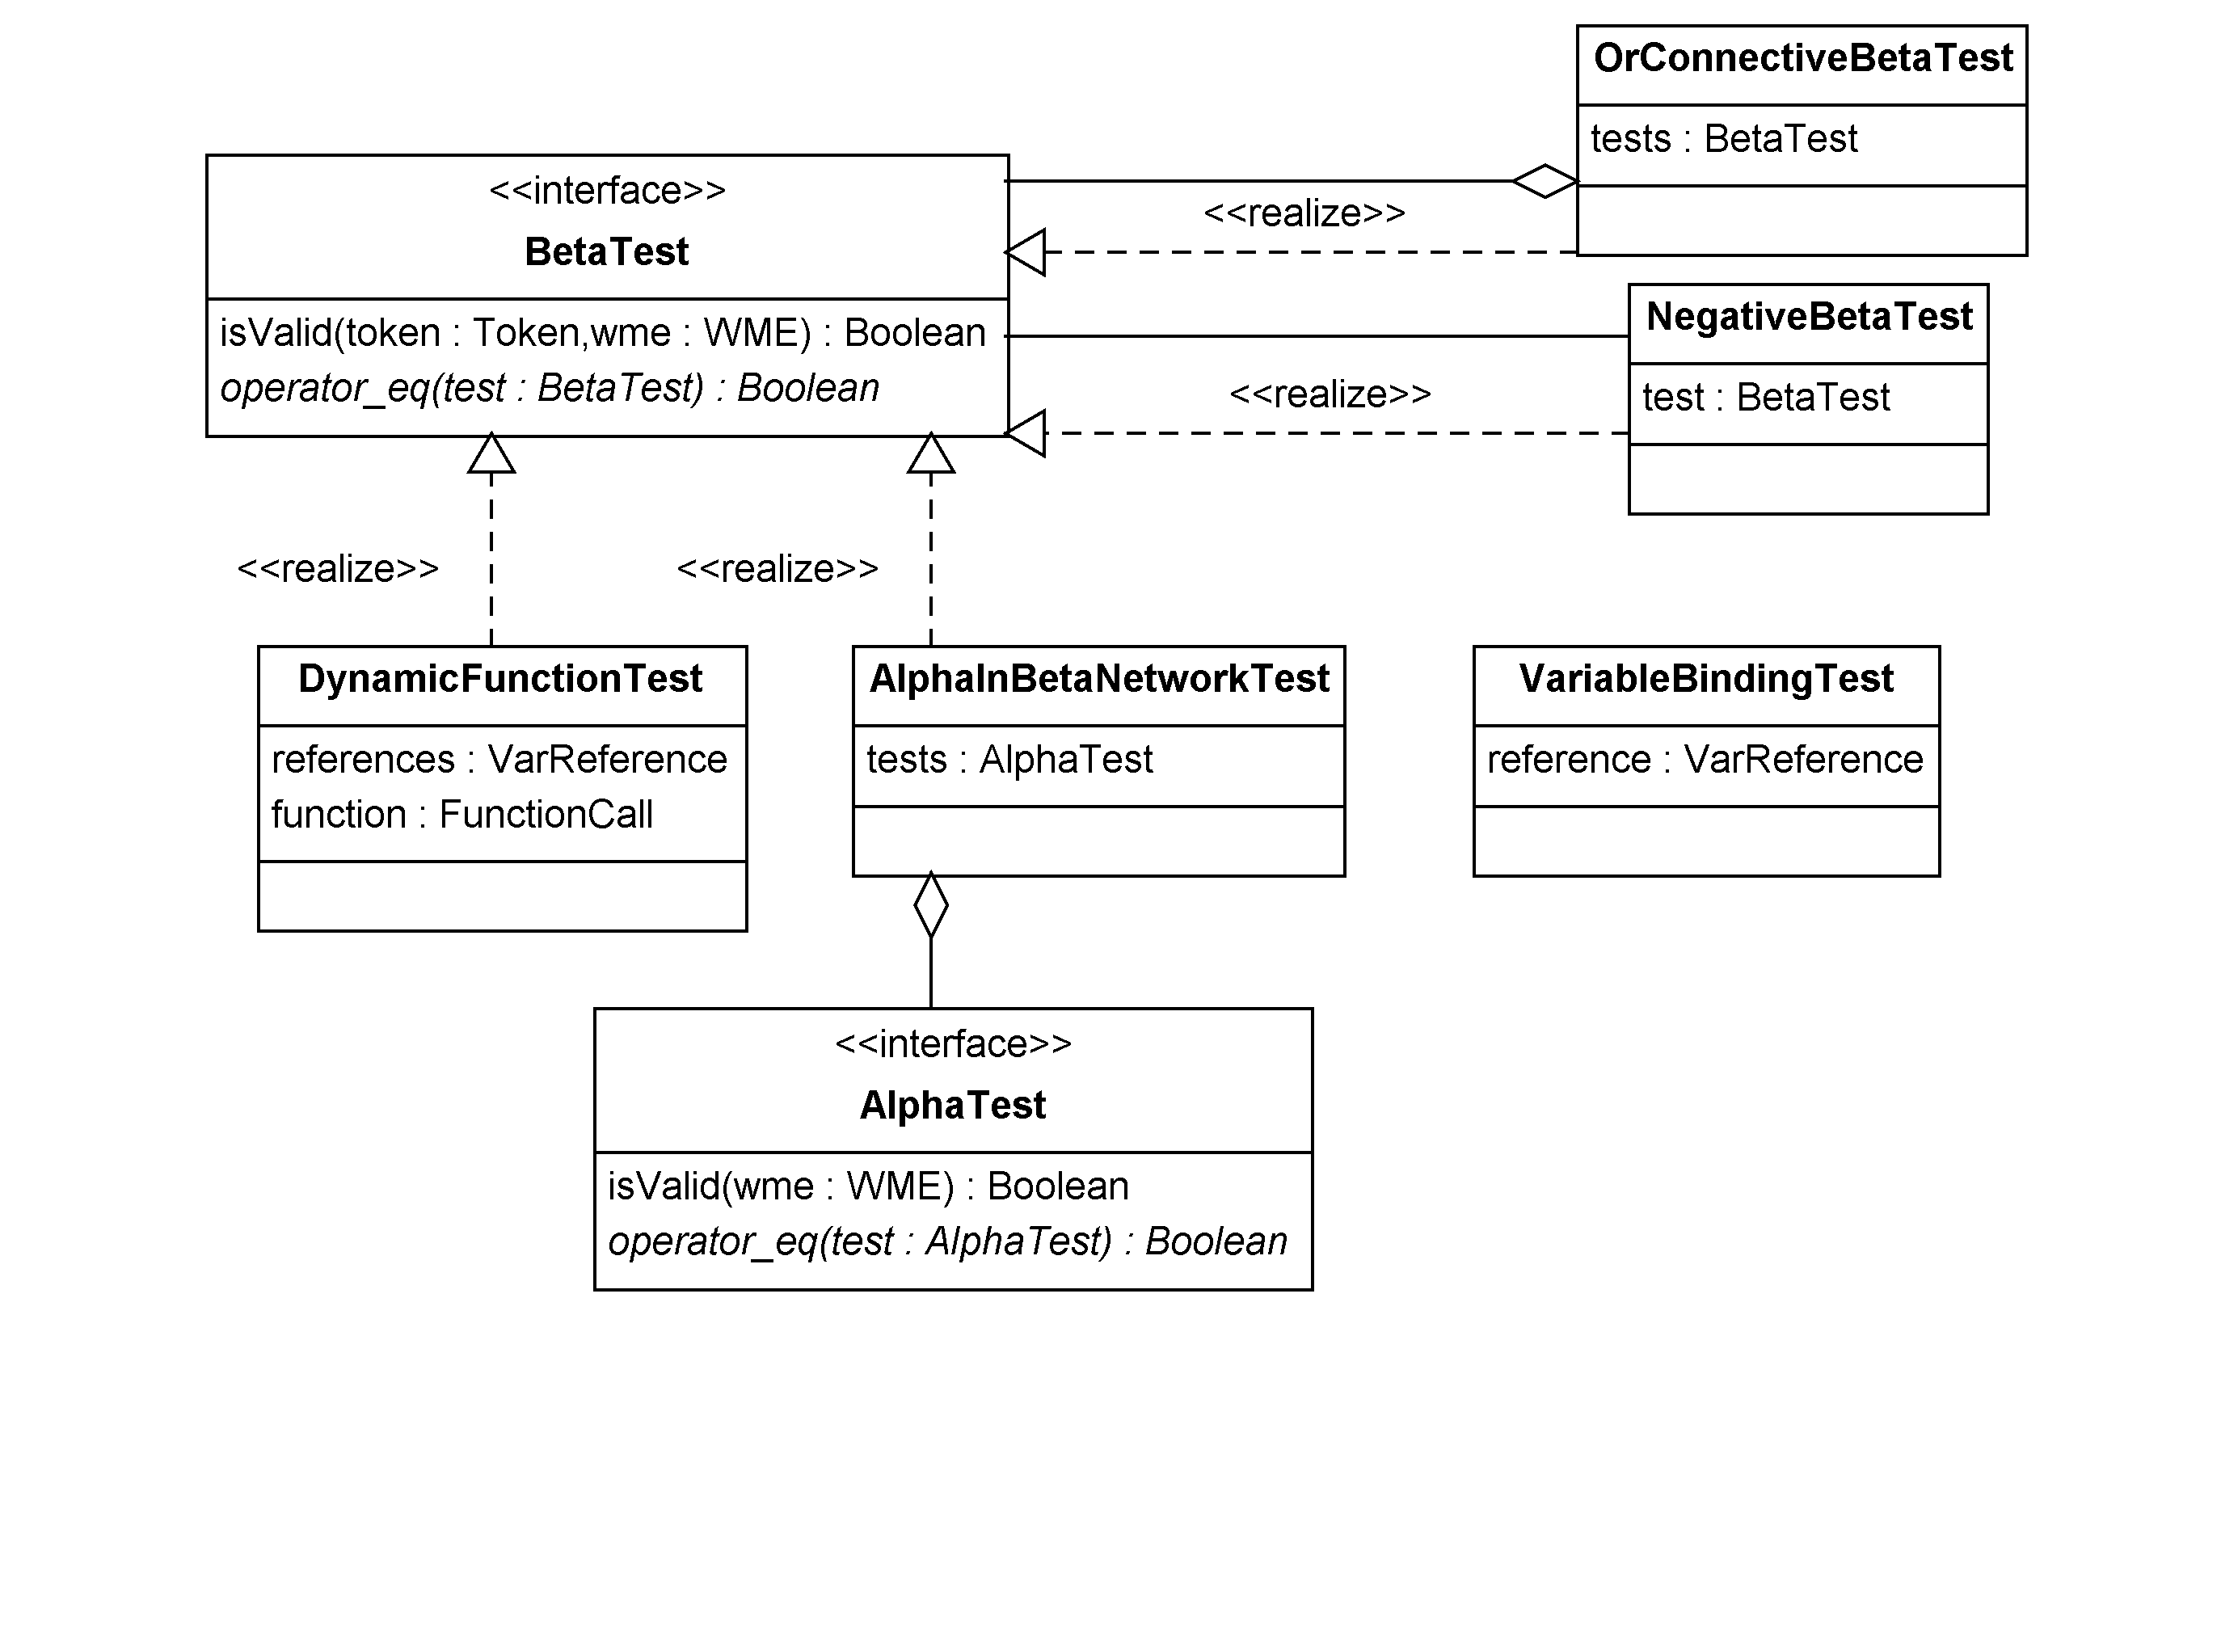
\includegraphics[width=1\textwidth]{Immagini/Capitolo3/Classi/myclips_rete_tests_Beta.png}
\caption{Package \emph{myclips.rete.tests}: vista dei test eseguiti nella porzione \emph{beta}}\label{fig:class-myclips-rete-tests-beta}
\end{figure}

La seconda tipologia (\figurename~\ref{fig:class-myclips-rete-tests-beta}) esegue verifiche su gruppi di \emph{WME}, rappresentati da \emph{Token}, valutando la coerenza del valore di variabili comuni a più pattern, il risultato dell'esecuzione di funzioni o valutando i risultato di test di tipo \emph{alpha} eseguiti nella porzione \emph{beta} del grafo. Al fine di poter eseguire i test di tipo \emph{alpha} nei nodi di tipo \emph{beta} è stata adottata una strategia facente riferimento al \emph{design pattern} strutturale \emph{Adapter} (anche noto con il nome di \emph{Wrapper} o \emph{Translator}): la classe \emph{AlphaInBetaNetworkTest}, che realizza l'interfaccia \emph{BetaTest}, incapsula oggetti con interfaccia \emph{AlphaTest} al suo interno. Le operazioni di traduzione degli argomenti dei test vengono eseguite all'interno dell'implementazione della classe.



\clearpage

\subsubsection{Modulo Interprete}

\begin{figure}[h]
\centering
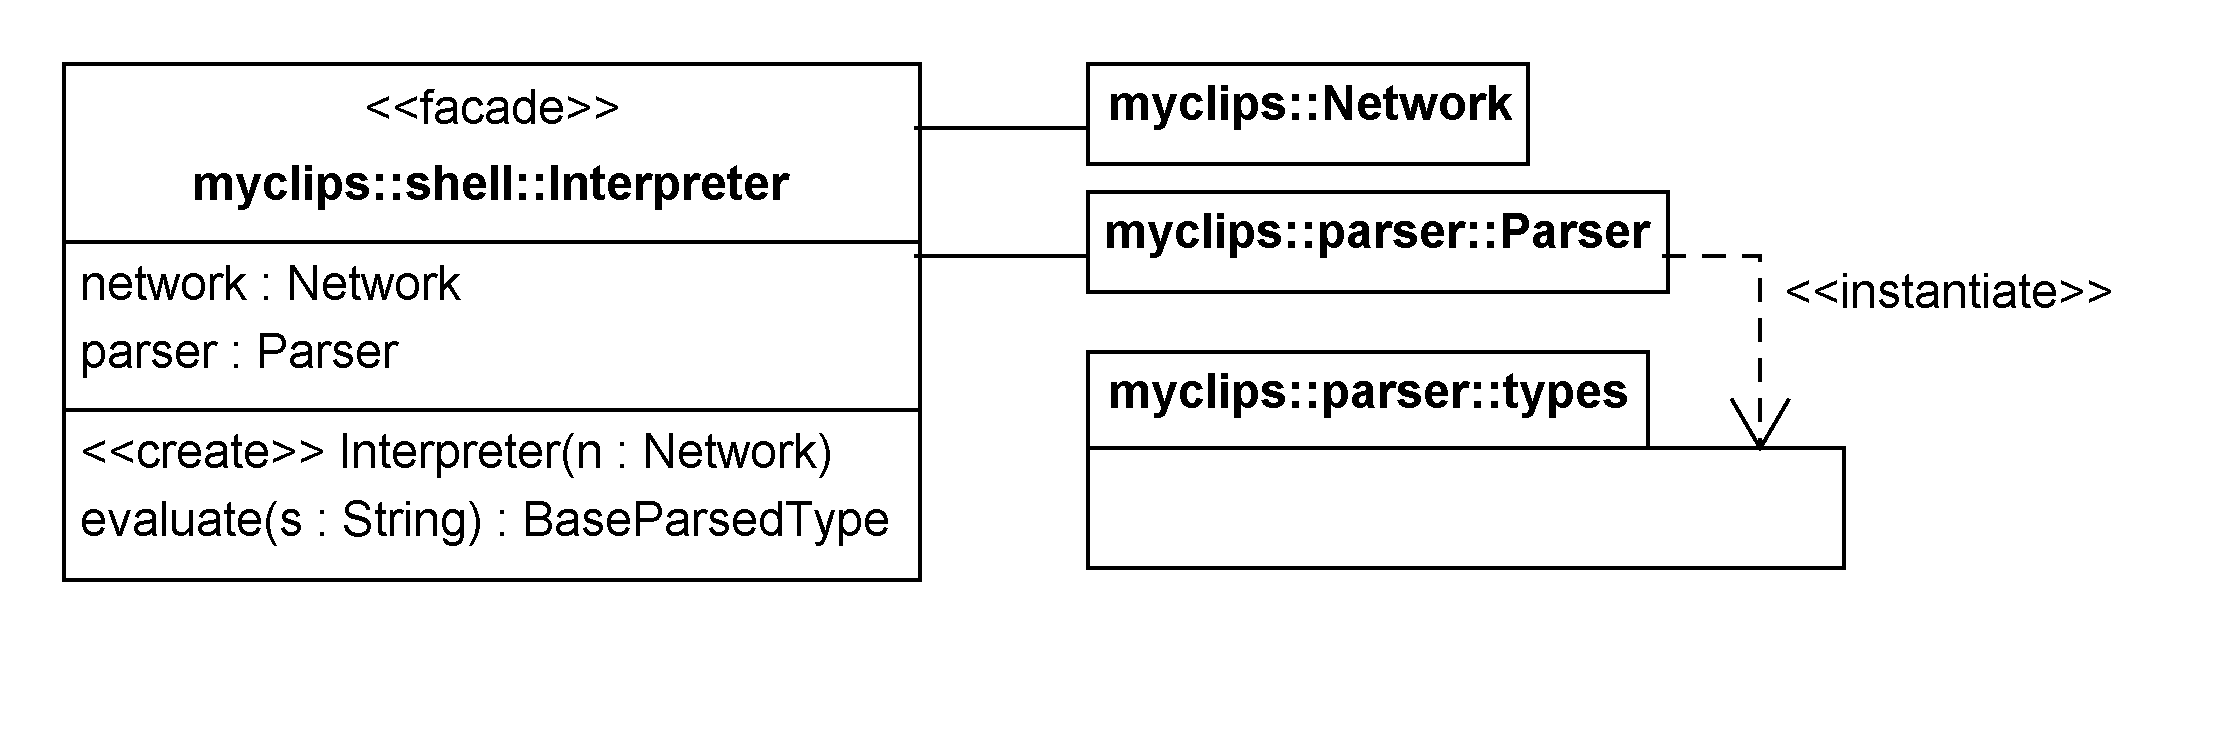
\includegraphics[width=1\textwidth]{Immagini/Capitolo3/Classi/myclips_shell_Interpreter.png}
\caption{Package \emph{myclips.rete.shell}: vista della classe \emph{Interpreter}}\label{fig:class-myclips-shell-interpreter}
\end{figure}

Il modulo \emph{Interprete}, contenuto nel \emph{package} \emph{myclips.shell}, consiste di un'unica classe \emph{fa\c{c}ade}: \emph{Interpreter}. Lo scopo della classe è quello semplificare ed unificare le operazioni di \emph{parsing} e valutazione dei costrutti, associandole alle attività di inizializzazione del \emph{motore inferenziale} e all'esecuzione del ciclo principale~(\figurename~\ref{fig:class-myclips-shell-interpreter}).

L'unica attività svolta dall'\emph{Interpreter} è quella di inizializzare un'istanza del \emph{Parser}, richiedere la valutazione di stringhe rappresentanti singoli \emph{costrutti} o \emph{comandi} e, se necessario, avviare l'interpretazione del costrutto dal parte di un'istanza di \emph{Network}. Nel caso l'elemento valutato dal parser sia un \emph{comando} (una chiamata a funzione di sistema), l'interprete provvede all'esecuzione dello stesso.

\subsubsection{Modulo Events Manager}

\begin{figure}[h]
\centering
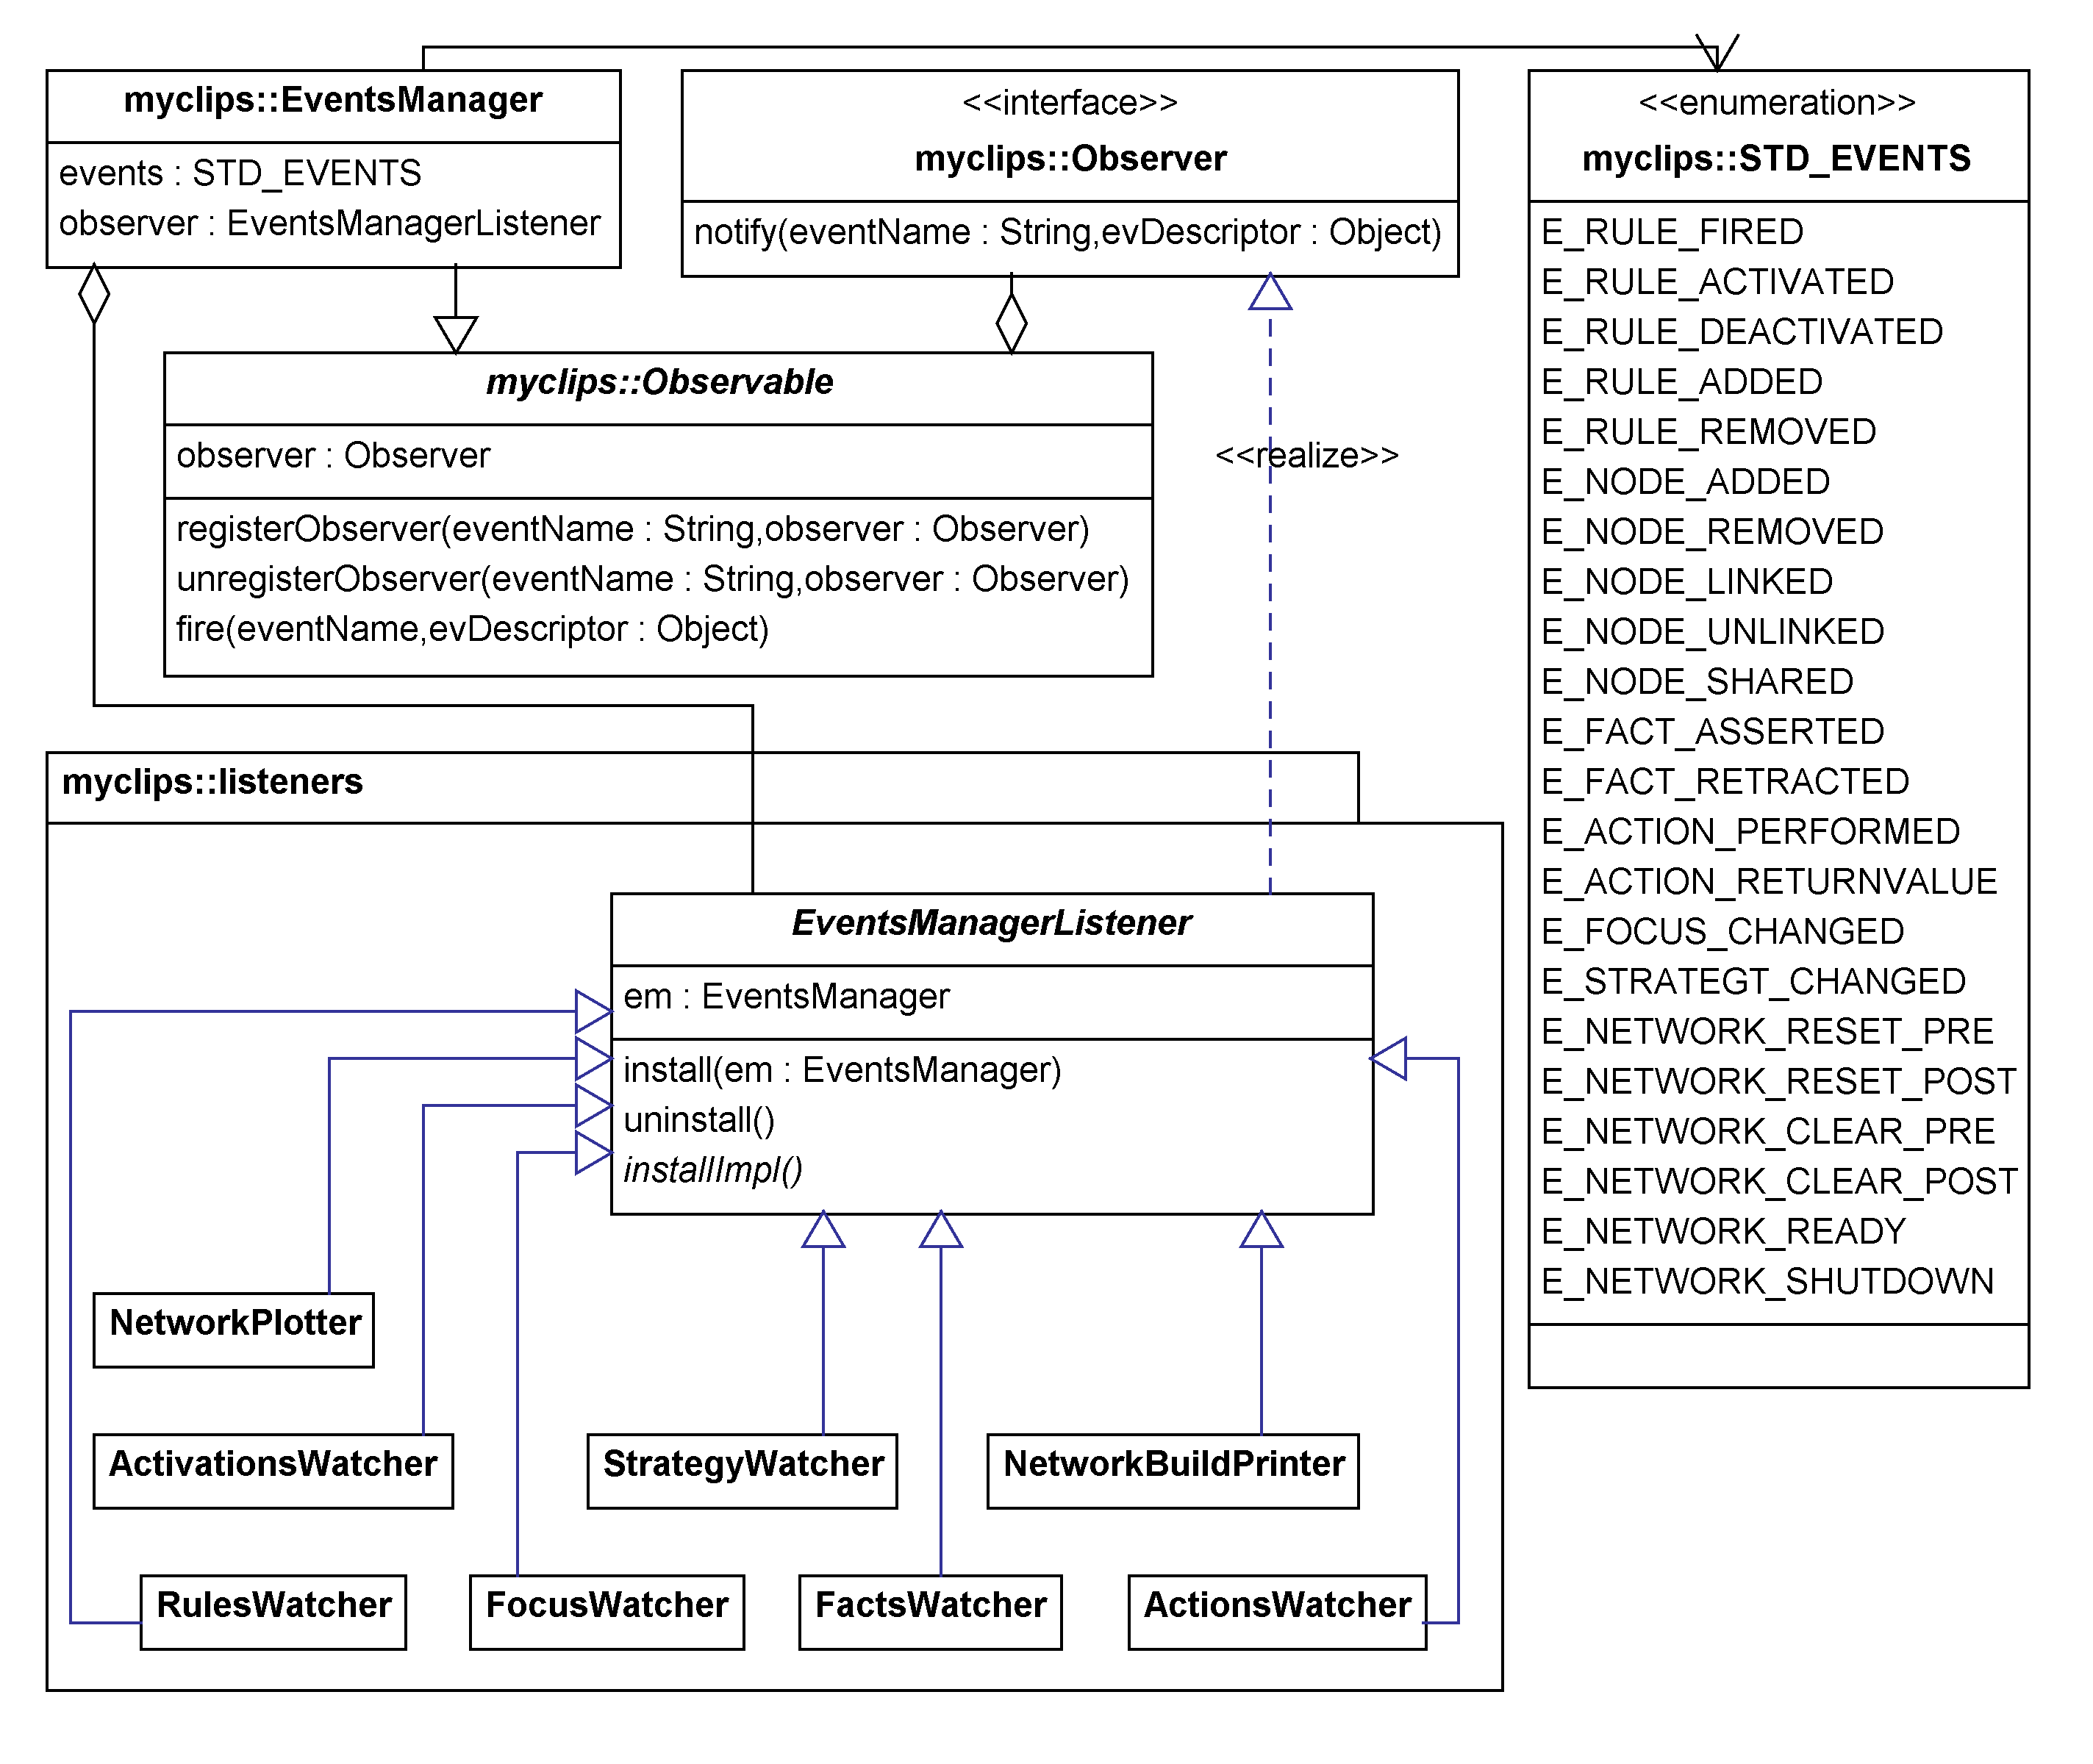
\includegraphics[width=1\textwidth]{Immagini/Capitolo3/Classi/myclips_EventsManager-Listeners.png}
\caption{Package \emph{myclips.rete.listeners}: vista della classi per la gestione degli eventi}\label{fig:class-myclips-eventsmanager}
\end{figure}

La gestione degli eventi è affidata alla collaborazione fra la classe \emph{EventsManager}, posta nel \emph{package} \emph{myclips}, e i \emph{listeners} riuniti nel \emph{package} \emph{myclips.listeners}~(\figurename~\ref{fig:class-myclips-eventsmanager}).

Usando come base l'infrastruttura offerta dallo schema \emph{Observer/Observable}, la classe \emph{EventsManager} viene utilizzata nel sistema per notificare il verificarsi di eventi. In aggiunta ad una serie di eventi predefiniti raggruppati in \emph{STD\_EVENTS}, la classe consente di notificare un qualsiasi evento personalizzato all'insieme di \emph{listener} registrati.

I \emph{listener} sono classi che estendono la classe astratta \emph{EventsManagerListener}. Il sistema fornisce un gruppo di definizioni predefinite con le quali intercettare gli eventi più comuni. Ogni classe, tramite la propria implementazione, esegue un comportamento differente come risposta ai singoli eventi per i quali si registra. La procedura di registrazione dei \emph{listener} è effettuata all'interno del metodo \emph{EventsManagerListener::install}, alle super-classi viene offerta la possibilità di personalizzare la procedura tramite l'implementazione del metodo \emph{EventsManagerListener::installImpl}, realizzando in questo modo lo schema previsto dal \emph{design pattern} comportamentale \emph{Template method}.

\subsubsection{Modulo Funzioni}
Il \emph{package} \emph{myclips.functions} gestisce la collezione di funzioni di sistema, così come l'intera infrastruttura per la manipolazione della stessa~(\figurename~\ref{fig:class-myclips-functions}).

\begin{figure}
\centering
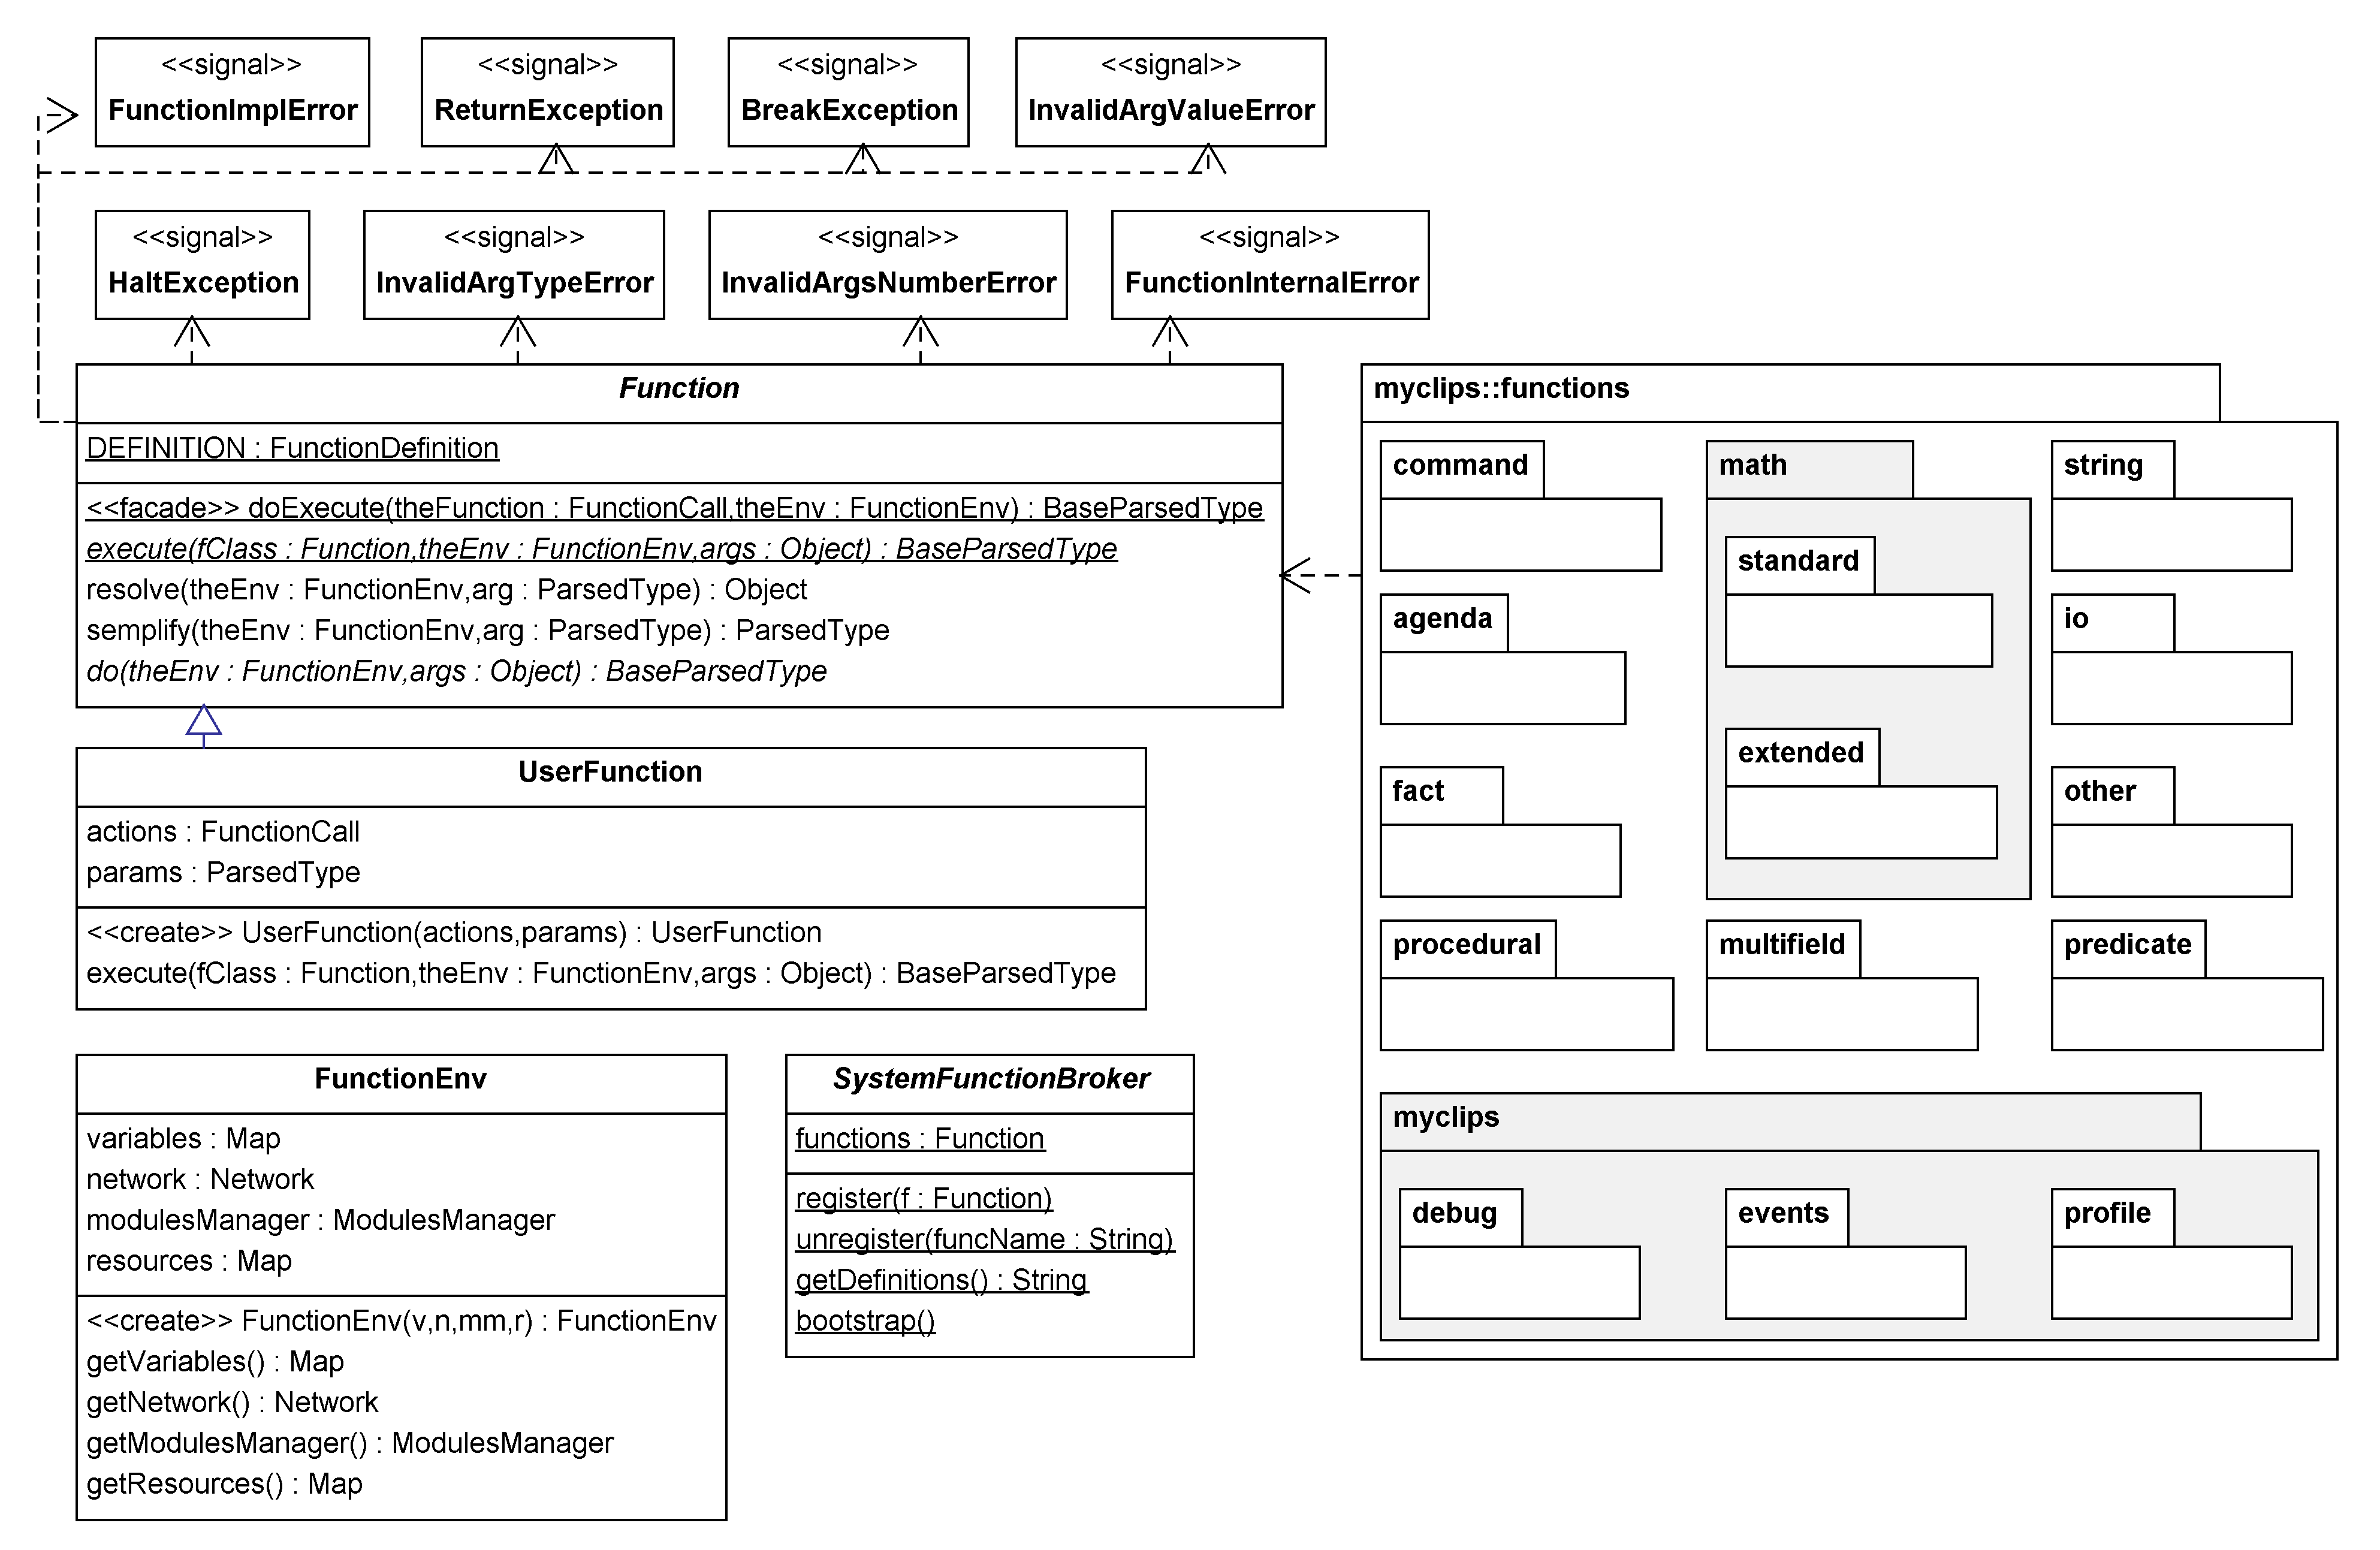
\includegraphics[width=1.3\textwidth, angle=270]{Immagini/Capitolo3/Classi/myclips_functions-Globale.png}
\caption{Package \emph{myclips.rete.functions}: vista della classi per la gestione delle funzioni di sistema}\label{fig:class-myclips-functions}
\end{figure}

Alla base di ogni funzione di sistema c'è la classe astratta \emph{Function}, la quale realizza una strategia basata sul \emph{design pattern} comportamentale \emph{Command}. Il contesto d'esecuzione delle funzioni viene fornito attraverso un'istanza di classe \emph{FunctionEnv}, la quale conserva riferimenti al \emph{Network}, \emph{ModulesManager} e alle risorse inizializzate dal sistema (l'elenco di \emph{stream di input/output}).

La base per la gestione delle definizioni è offerta dal \emph{SystemFunctionBroker}: definisce metodi per l'aggiunta o la rimozione di definizioni a \emph{run-time}, cosi come implementa il meccanismo automatico di caricamento delle definizioni partendo da un registro conservato su \emph{file} (tramite il metodo \emph{bootstrap}).

L'elenco di funzioni di sistema è distribuito all'interno del \emph{sub-package} \emph{myclips.function}. L'organizzazione adottata rispecchia la tipologia di funzioni. Le classi definite nel \emph{sub-package} \emph{myclips.functions.myclips} rappresentano funzioni originali del sistema MyCLIPS per la gestione di eventi e la valutazione degli artefatti (sia dal punto di vista prestazionale che di correttezza). Le restanti definizioni realizzano funzioni previste da CLIPS: le sintassi e le semantiche delle definizioni rispecchiano quelle previste dal software CLIPS per consentire la portabilità degli artefatti fra i sistemi.

\subsection{Server}

\begin{figure}[h]
\centering
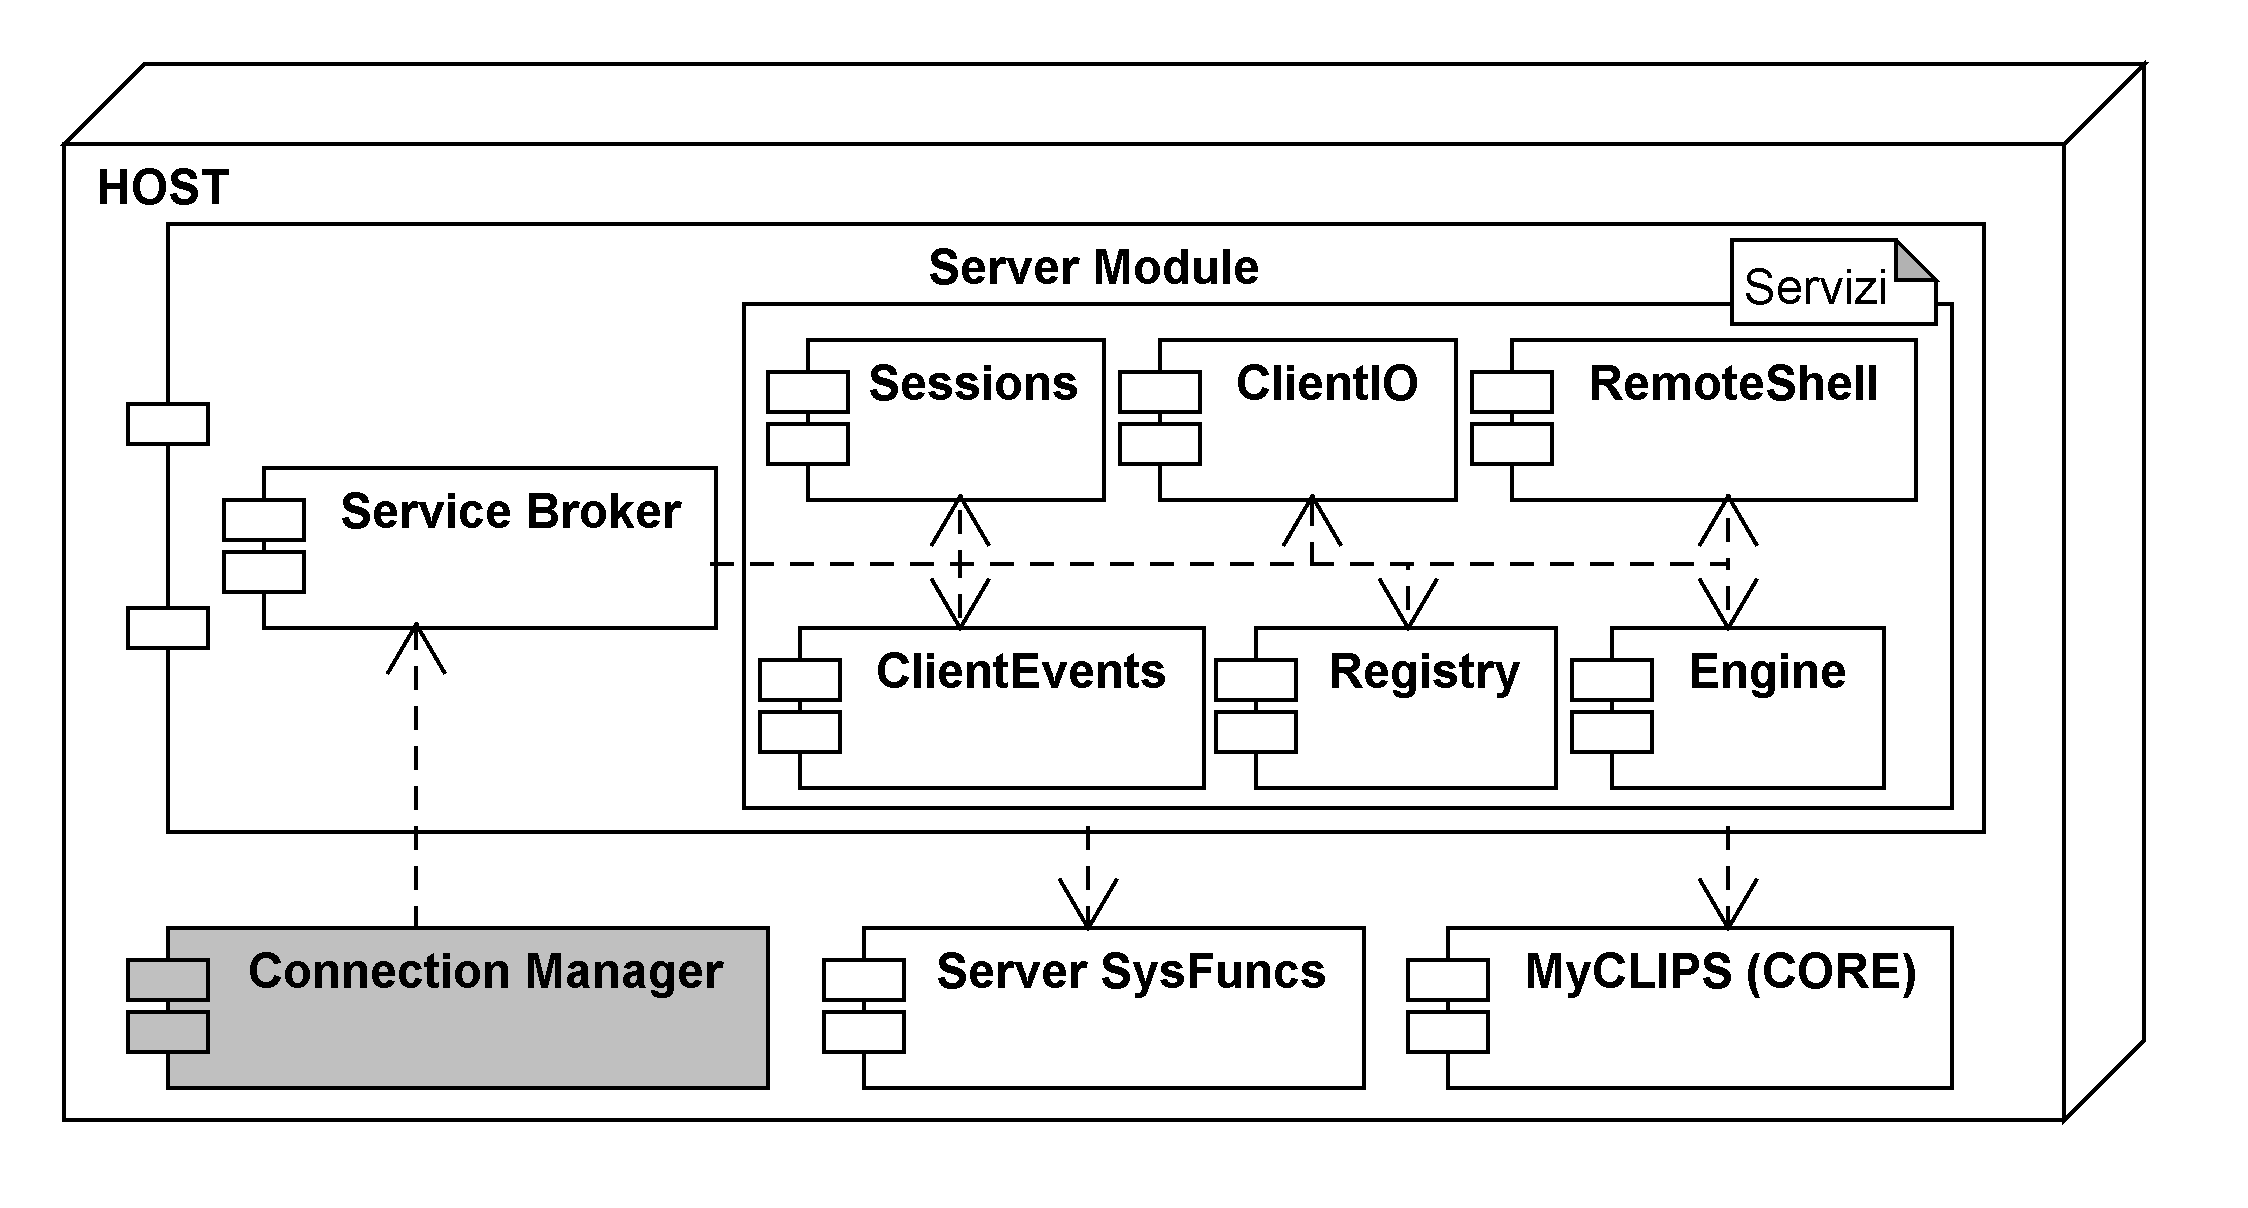
\includegraphics[width=1\textwidth]{Immagini/Capitolo3/Deployment/Server.png}
\caption{Vista generale dell'architettura server}\label{fig:architettura-server}
\end{figure}

L'architettura del modulo server rispecchia uno schema orientato alla suddivisione delle attività svolte in servizi differenti e che realizzano specifiche tipologie di interfaccia~(\figurename~\ref{fig:architettura-server}). Alla base delle implementazioni dei differenti servizi viene posto il componente software principale MyCLIPS.

\subsubsection{Broker di servizi}

\begin{figure}
\centering
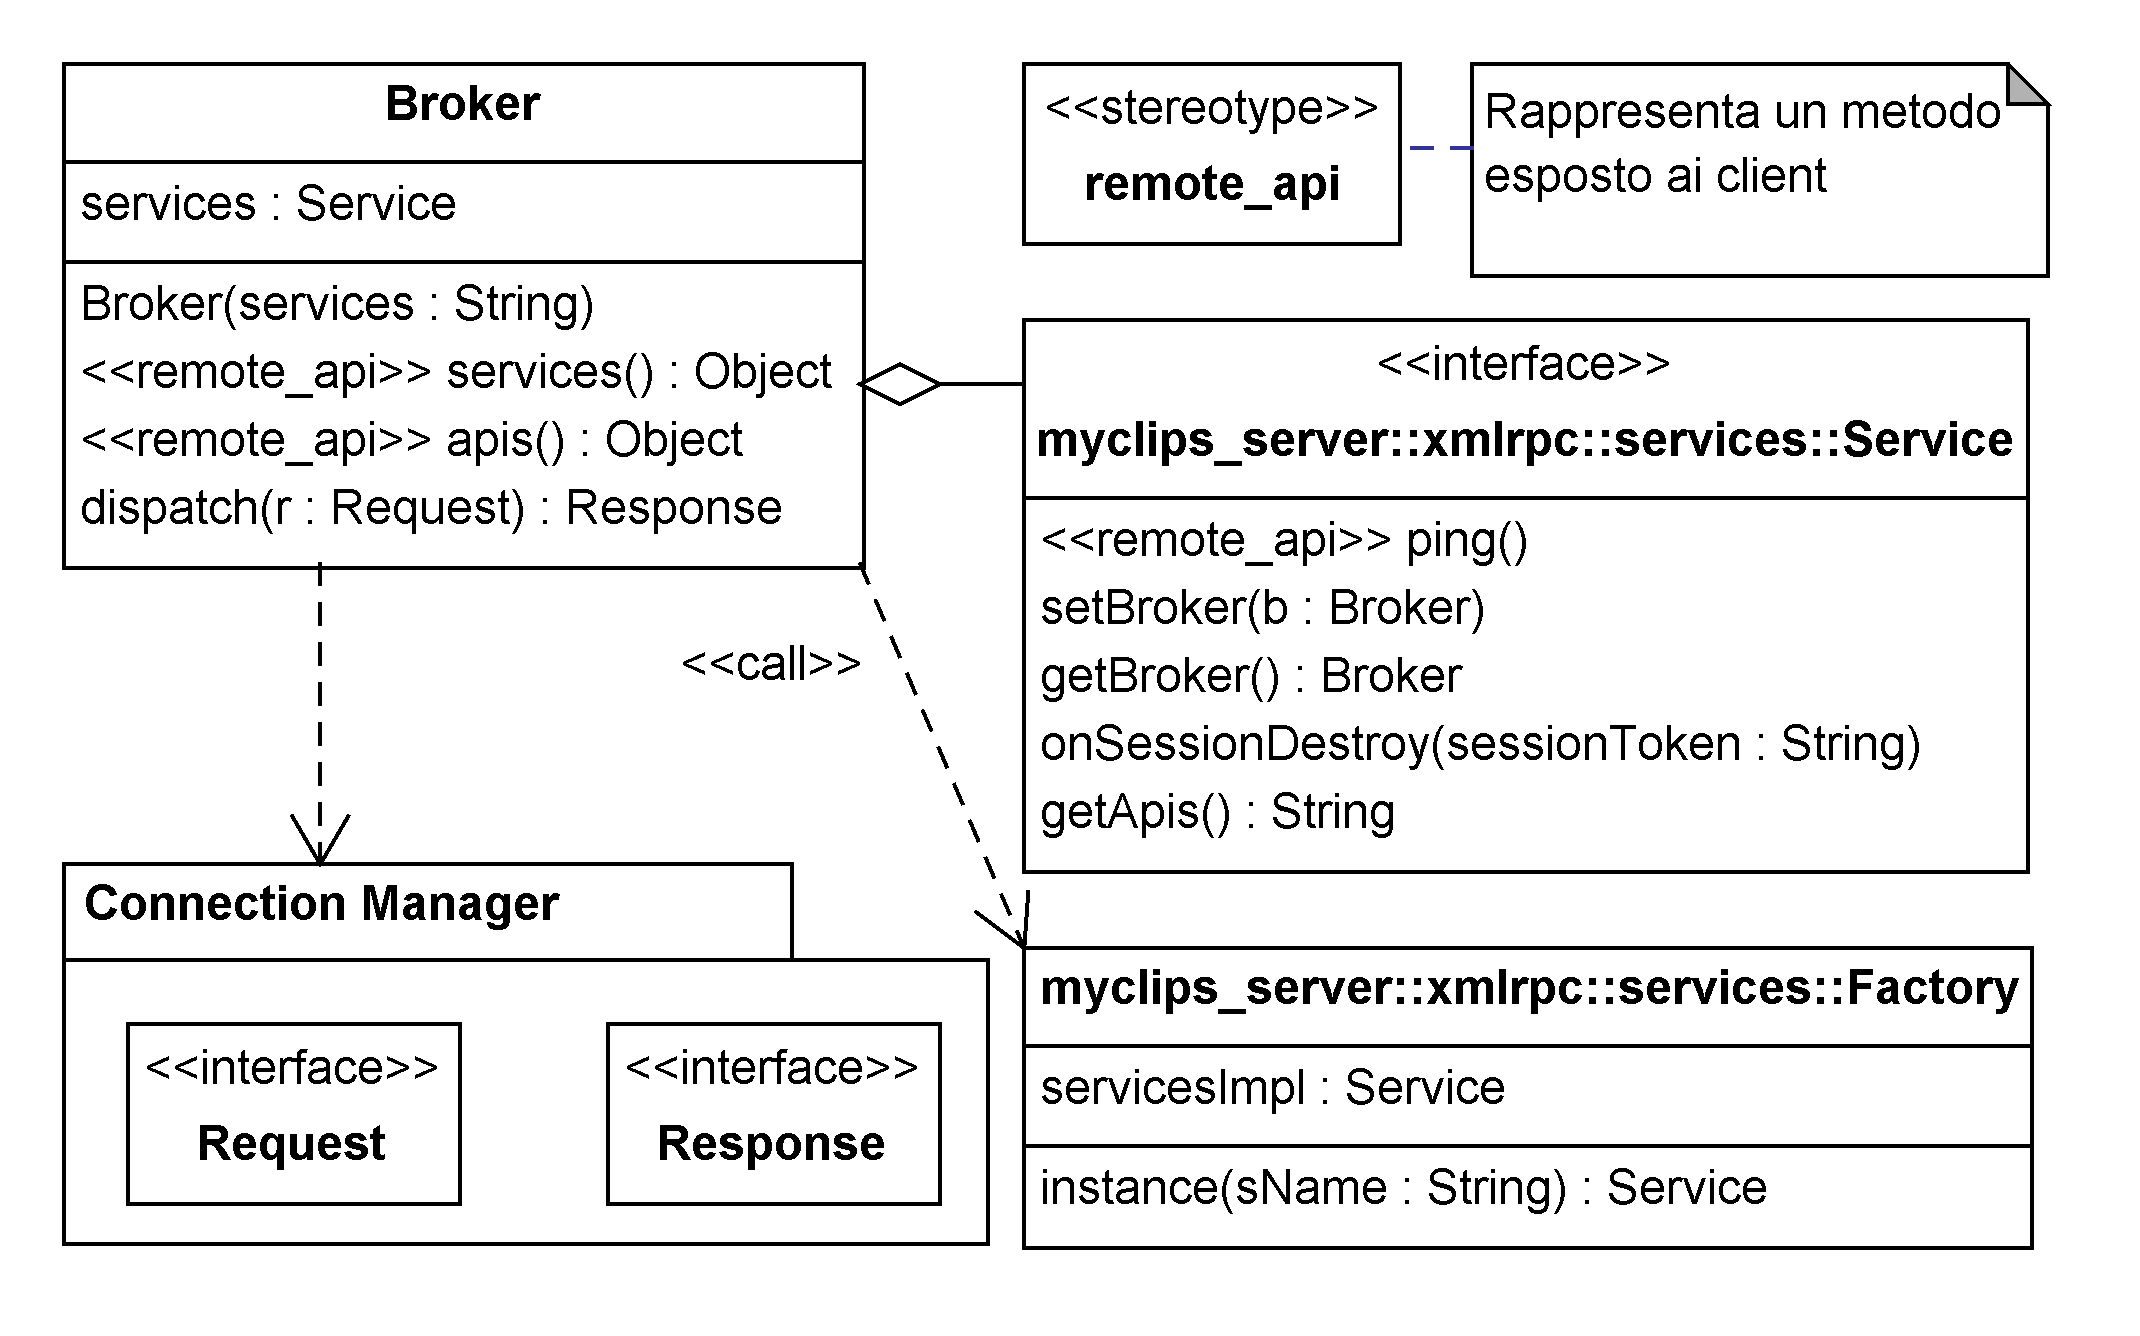
\includegraphics[width=1\textwidth]{Immagini/Capitolo3/Classi/myclips_server_Broker.png}
\caption{Package \emph{myclips\_server}: vista delle classi e interfacce relative al \emph{Broker}}\label{fig:class-myclips-server-broker}
\end{figure}

Il componente \emph{Broker}~(\figurename~\ref{fig:class-myclips-server-broker}) ha il compito di organizzare i servizi offerti dal modulo \emph{server}, controllando il flusso di richieste e risposte provenienti dall'infrastruttura addetta alla gestione delle connessioni con i client.

La realizzazione dell'interfaccia \emph{Service}, richiesta ad ogni classe concreta di servizio, garantisce l'implementazione dei metodi necessari alla registrazione della classe nel \emph{Broker}. L'interfaccia viene ulteriormente estesa da ogni tipologia specifica di servizio.

La creazione delle istanze concrete dei servizi viene delegata alle funzioni del \emph{Service Factory} (classe \emph{Factory} in \figurename~\ref{fig:class-myclips-server-broker})

\subsubsection{Servizio Sessioni}

\begin{figure}
\centering
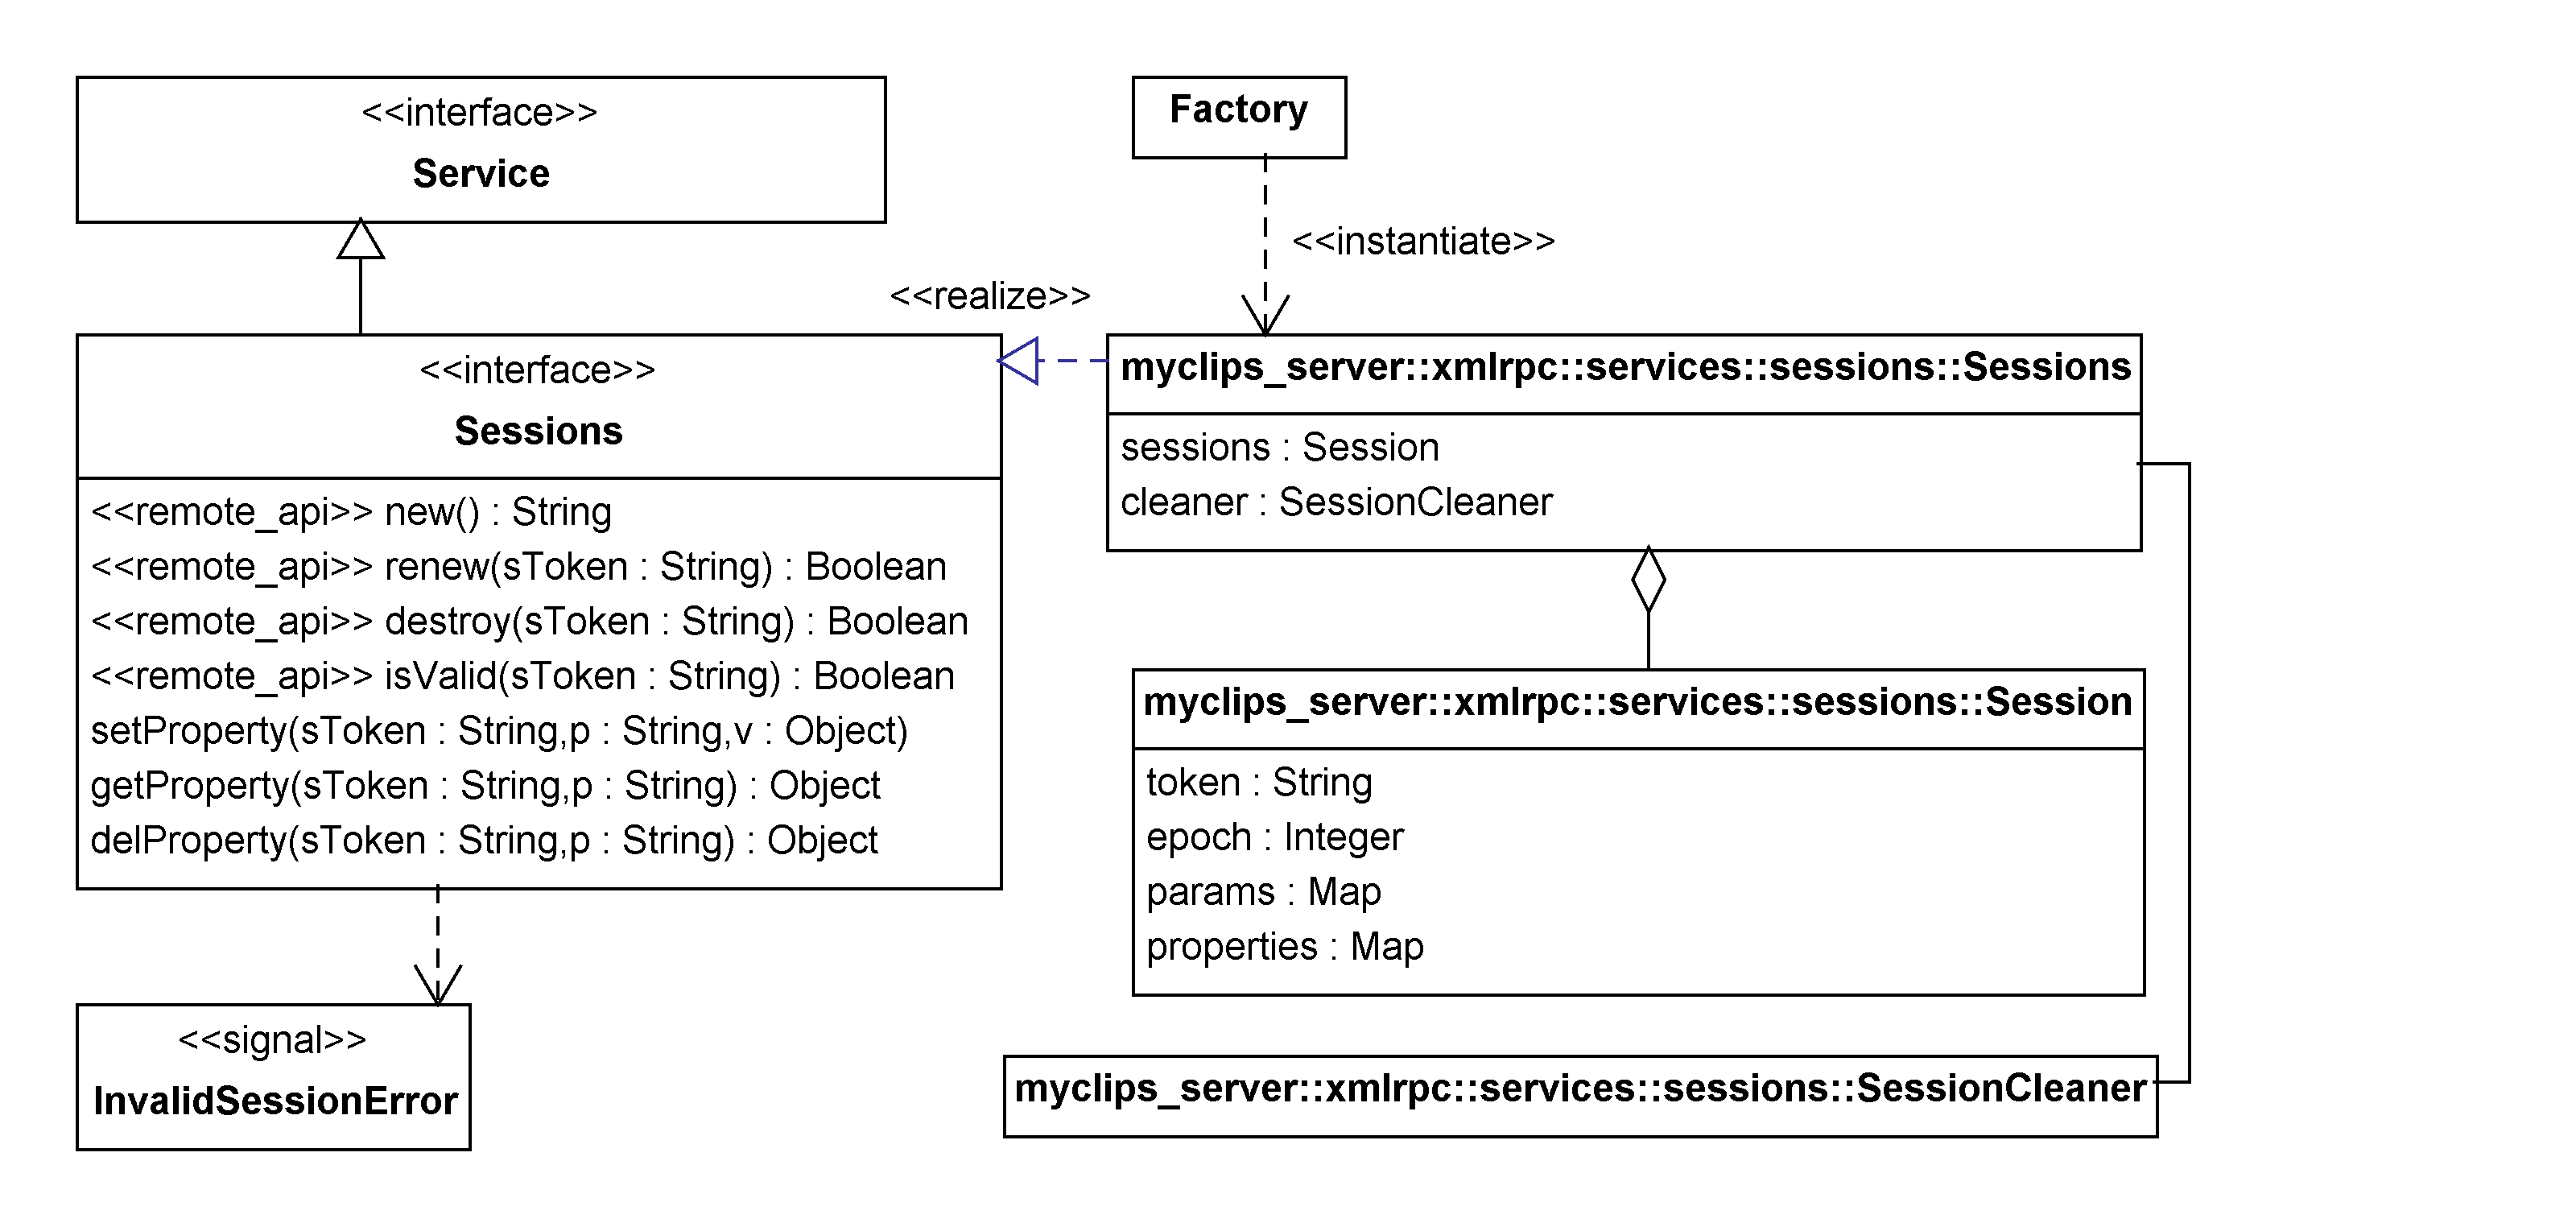
\includegraphics[width=1\textwidth]{Immagini/Capitolo3/Classi/myclips_server_services_Sessions.png}
\caption{Package \emph{myclips\_server.xmlrpc.services}: vista delle classi e interfacce relative al servizio \emph{Sessions}}\label{fig:class-myclips-server-services-sessions}
\end{figure}

Il servizio \emph{Sessions}~(\figurename~\ref{fig:class-myclips-server-services-sessions}) consente ai \emph{client} di creare sessioni persistenti fra più richieste successive. Ogni sessione viene inizializzata e gestita dalla classe concreta, che provvederà a memorizzarla fino a quando non verranno riscontrate condizioni favorevoli all'eliminazione.
Il servizio fornisce sia un'interfaccia rivolta ai client (per la creazione, rimozione e rinnovo delle sessioni), sia ad altri servizi del sistema (per realizzare un meccanismo di stoccaggio persistente delle informazioni).


\subsubsection{Servizio Registro di tipi}

\begin{figure}[h]
\centering
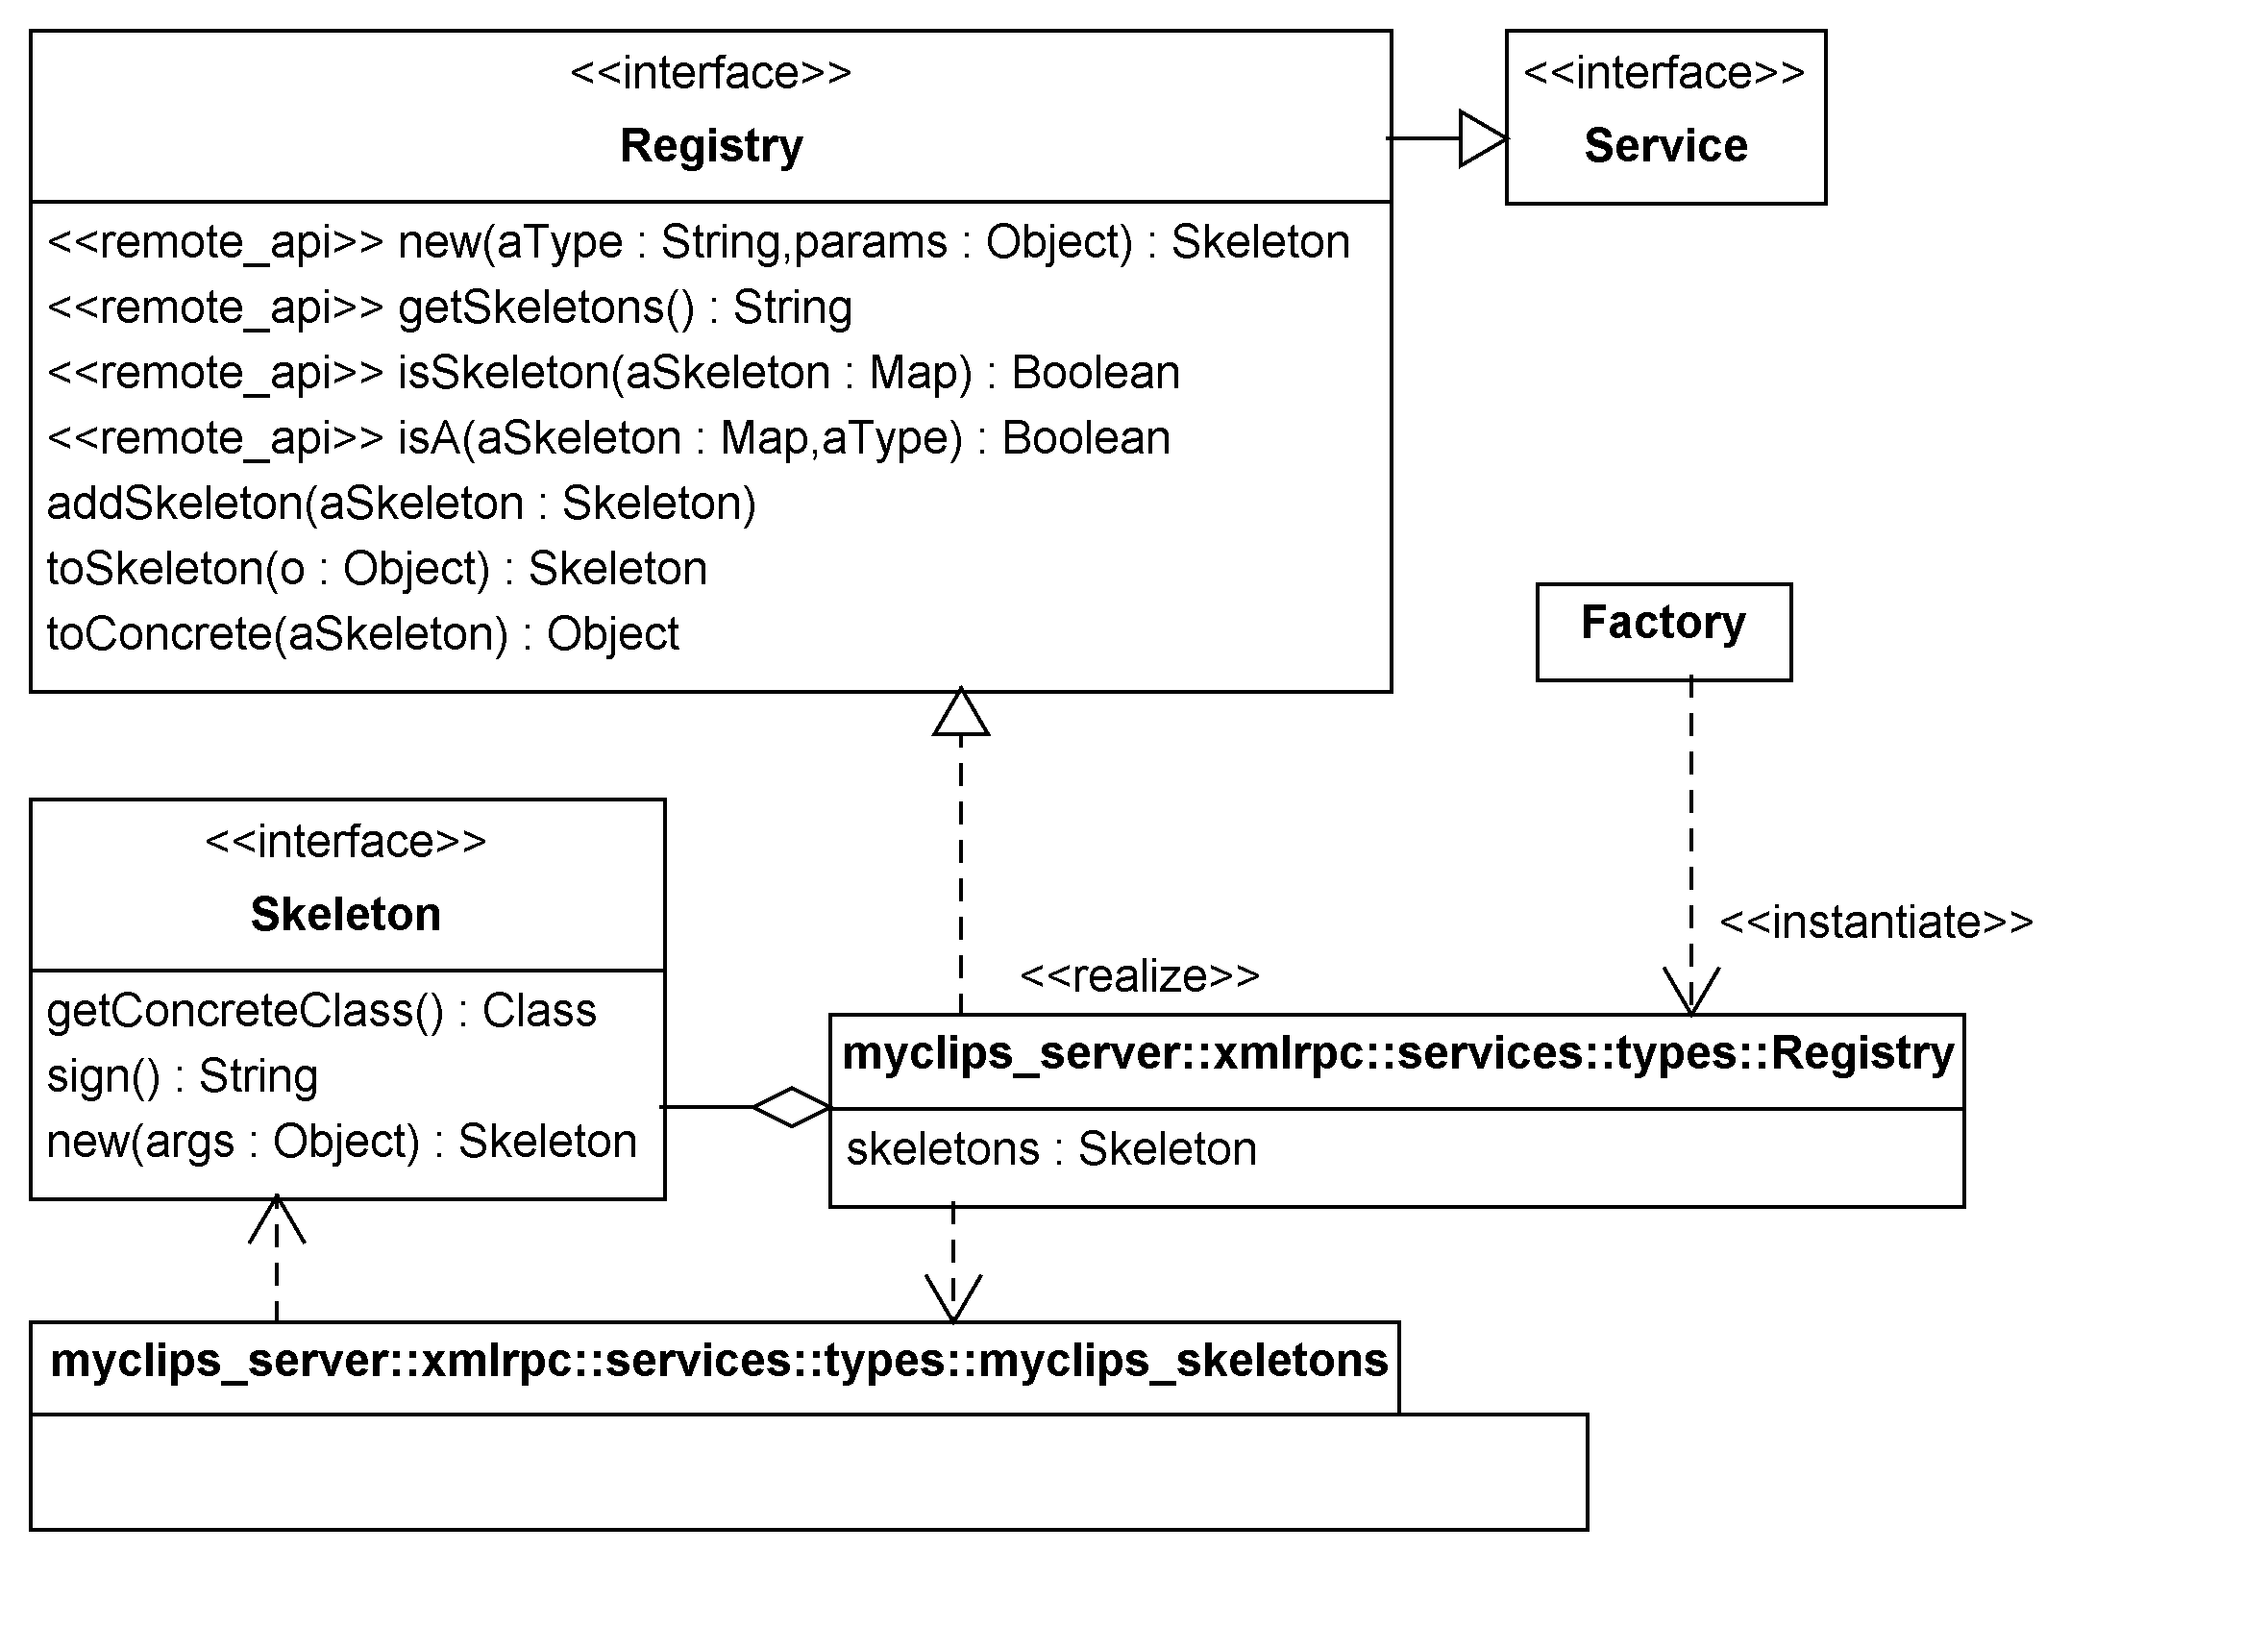
\includegraphics[width=1\textwidth]{Immagini/Capitolo3/Classi/myclips_server_services_Registry.png}
\caption{Package \emph{myclips\_server.xmlrpc.services}: vista delle classi e interfacce relative al servizio \emph{Registry}}\label{fig:class-myclips-server-services-registry}
\end{figure}

Il servizio \emph{Registry}~(\figurename~\ref{fig:class-myclips-server-services-registry}) consente, a client e altri servizi, di manipolare tipi complessi non previsti da specifiche implementazioni del protocollo di trasmissione dei messaggi fra \emph{client} e \emph{server}. Le attività svolte dal servizio sono quelle di organizzare una collezione di classi \emph{Skeleton} che forniscano i metodi di conversione da classi specifiche a forme di più facile trasmissione e viceversa.
Il servizio offre anche la possibilità ad altre parti del sistema di registrare tipi di \emph{Skeleton} personalizzati.

L'implementazione concreta dell'interfaccia del servizio, realizzata dalla classe \emph{Registry}, utilizza una collezione di \emph{Skeleton} riuniti nel \emph{sub-package} \emph{myclips\_server.xmlrpc.services.types.myclips\_skeletons} per rappresentare costrutti e tipi utilizzati dal motore inferenziale.

\subsubsection{Servizio Client IO}

\begin{figure}[h]
\centering
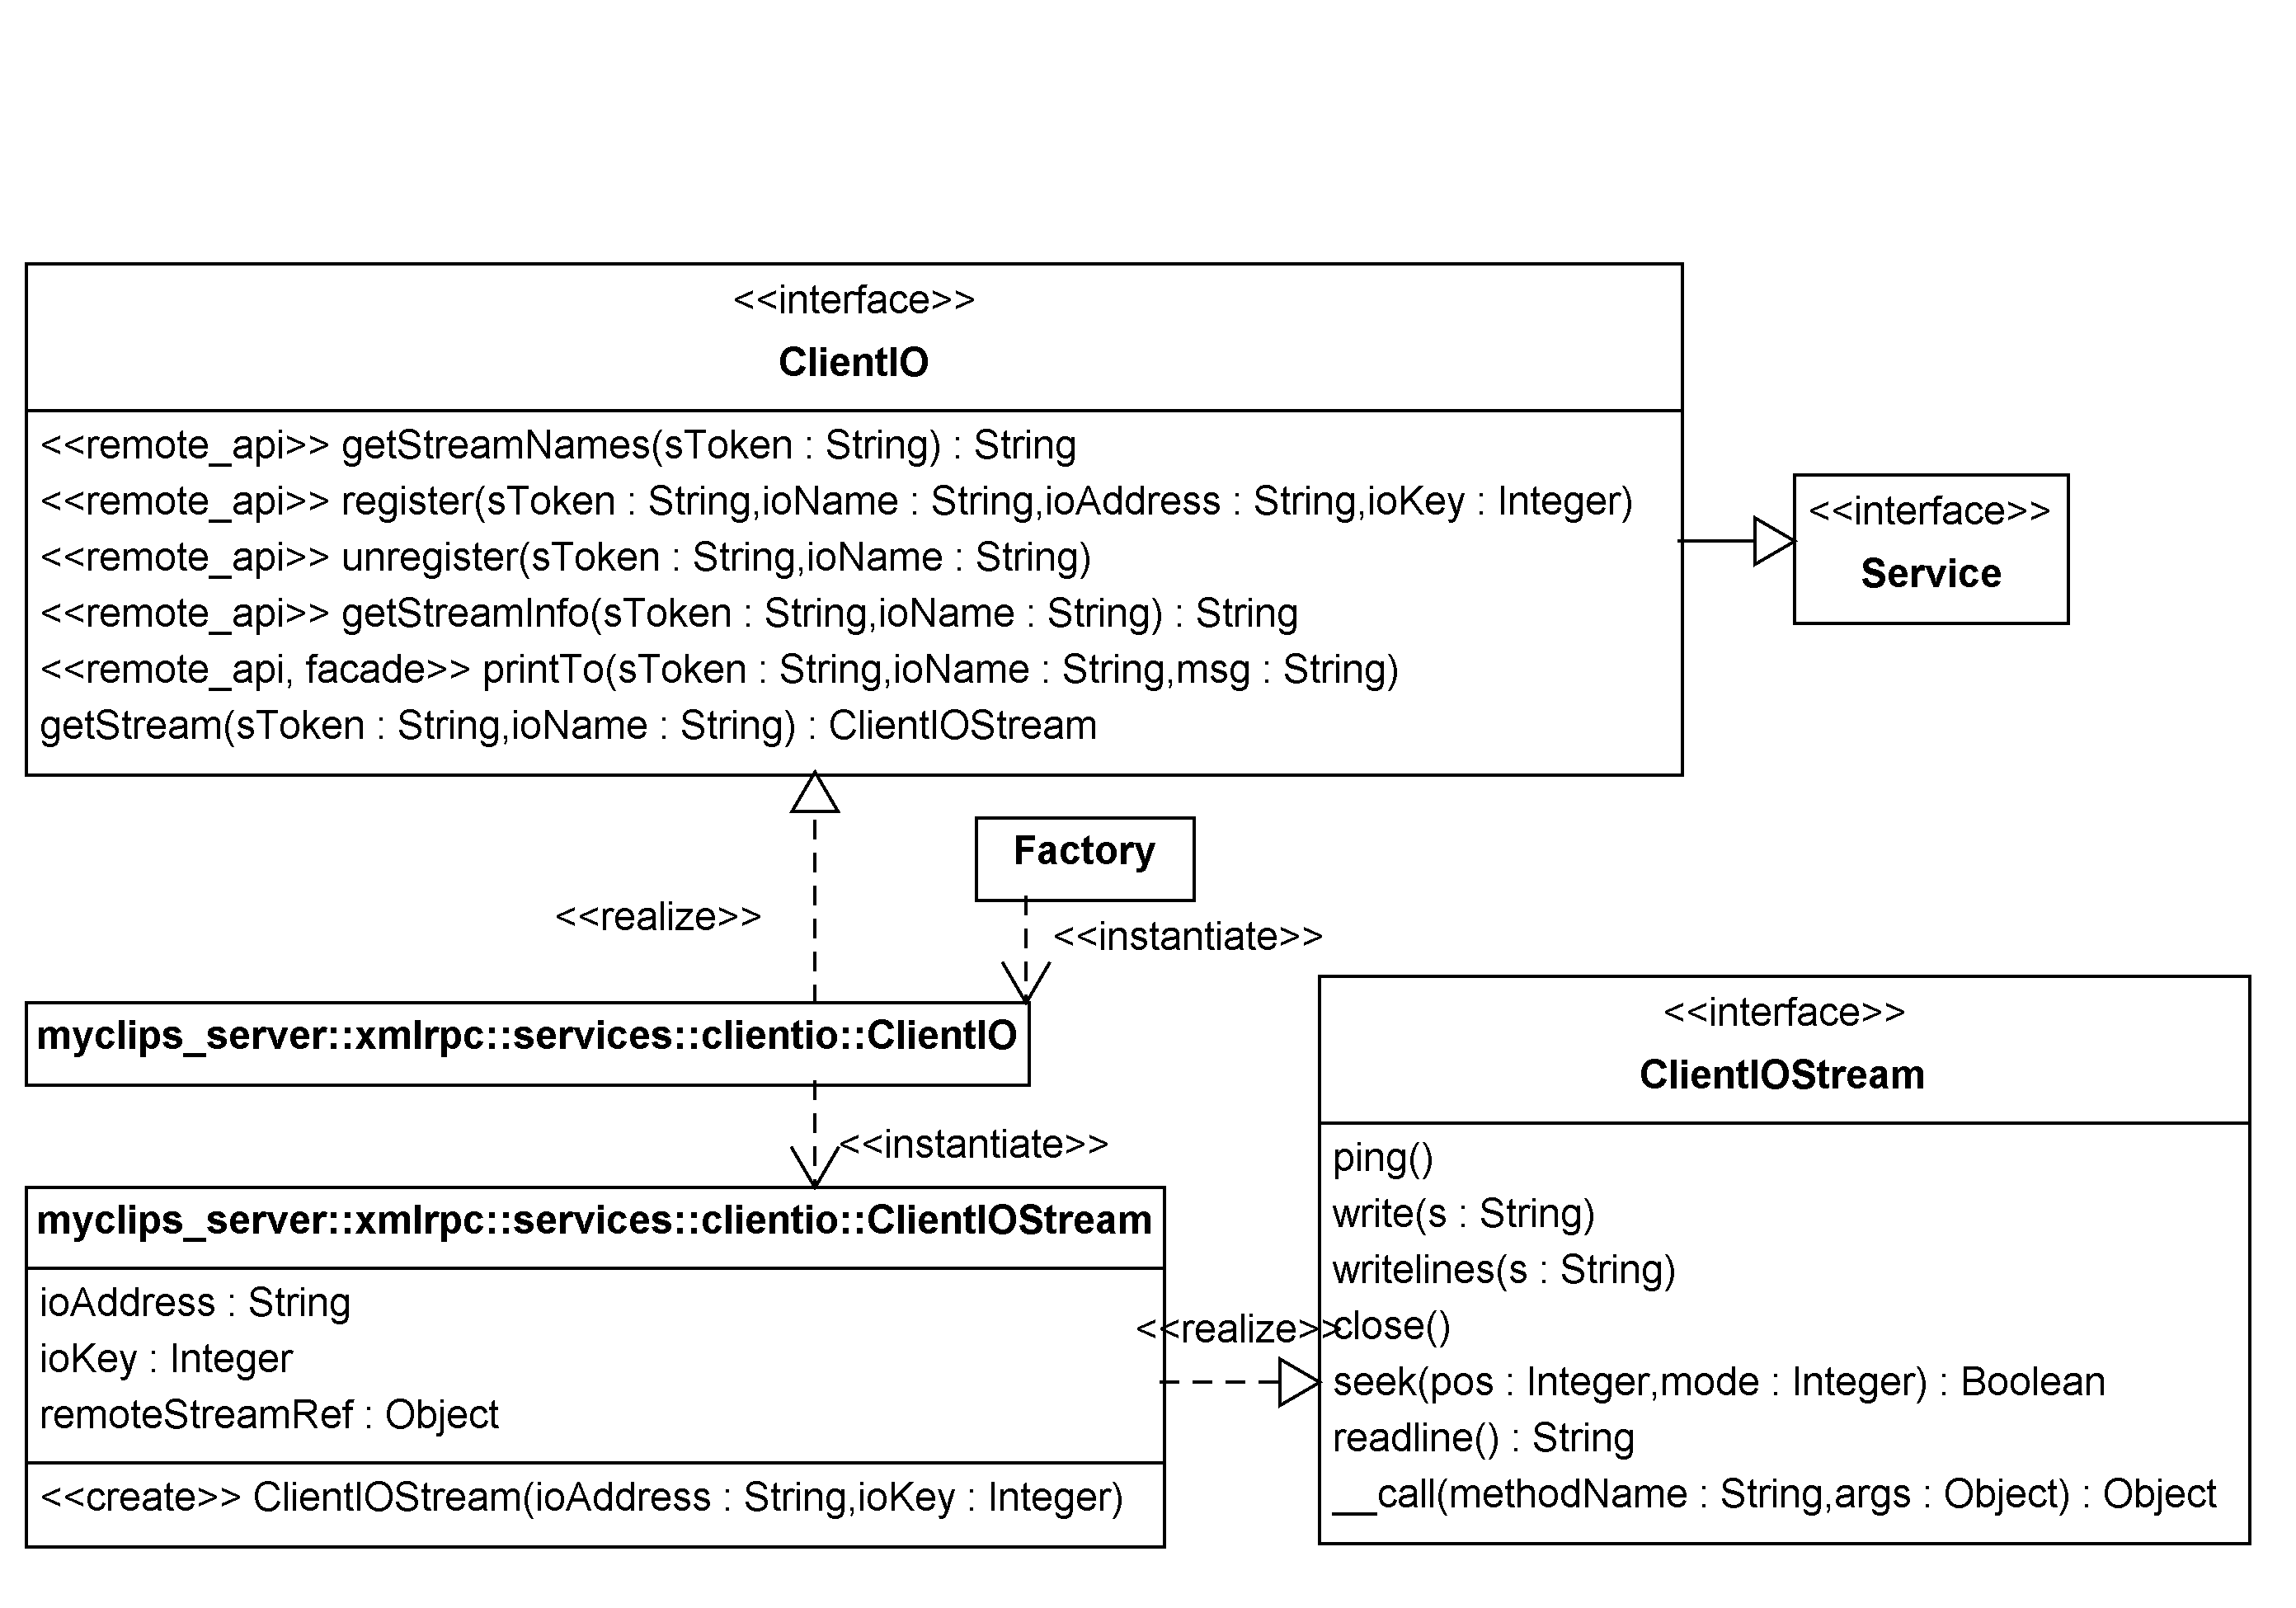
\includegraphics[width=1\textwidth]{Immagini/Capitolo3/Classi/myclips_server_services_ClientIO.png}
\caption{Package \emph{myclips\_server.xmlrpc.services}: vista delle classi e interfacce relative al servizio \emph{ClientIO}}\label{fig:class-myclips-server-services-clientio}
\end{figure}

Il servizio \emph{ClientIO}~(\figurename~\ref{fig:class-myclips-server-services-clientio}) permette ai client di fornire i parametri di utilizzo relativi a stream remoti che il server  (e i relativi servizi) può utilizzare in sostituzione degli stream locali. L'utilizzo degli stream remoti consente di dirottare tutte le normali operazioni di scrittura e lettura, eseguite all'interno del motore inferenziale, verso le risorse messe a disposizione dal client in maniera trasparente.
Al client viene richiesta l'implementazione di un'interfaccia analoga a \emph{ClientIOStream}.

\subsubsection{Servizio Remote Shell}

\begin{figure}[h]
\centering
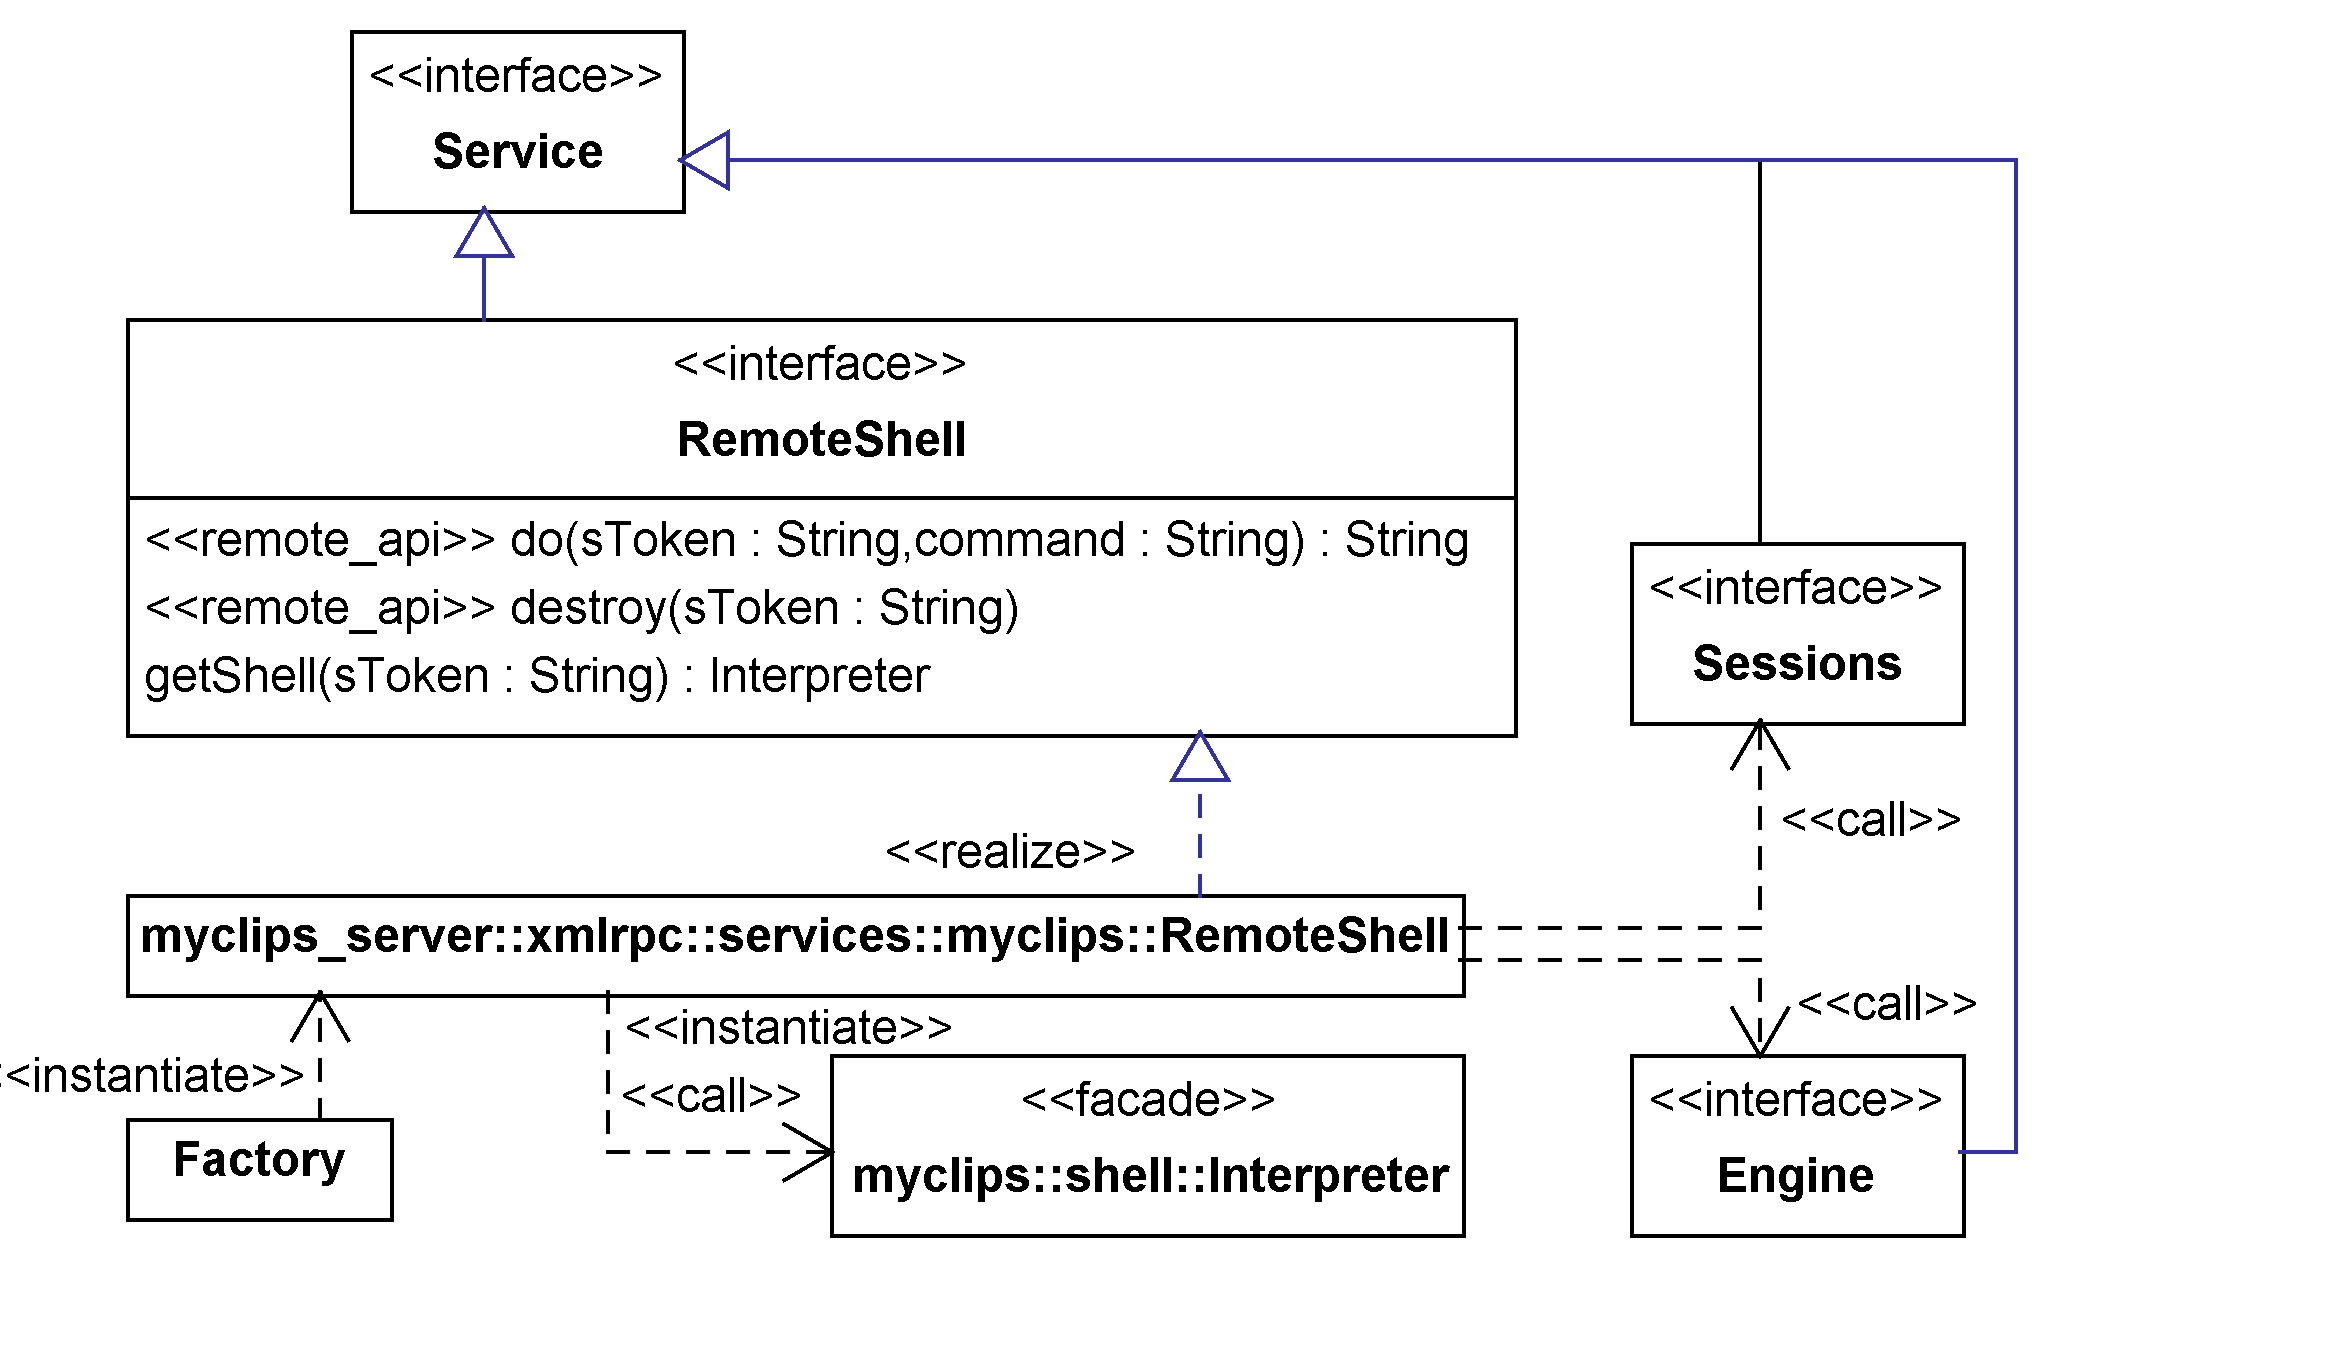
\includegraphics[width=1\textwidth]{Immagini/Capitolo3/Classi/myclips_server_services_RemoteShell.png}
\caption{Package \emph{myclips\_server.xmlrpc.services}: vista delle classi e interfacce relative al servizio \emph{RemoteShell}}\label{fig:class-myclips-server-services-remoteshell}
\end{figure}

Il servizio \emph{RemoteShell}~(\figurename~\ref{fig:class-myclips-server-services-remoteshell}) viene utilizzato per distribuire i servizi del modulo Interprete del sistema principale: attraverso lo scambio di comandi, trasferiti come stringhe di testo, è possibile manipolare istanze remote del motore inferenziale in maniera esattamente analoga a quanto avviene tramite l'utilizzo di un \emph{Terminale} locale.

Il servizio fa uso delle interfacce \emph{Sessions} (per memorizzare l'istanza \emph{Interpreter}), \emph{Engine} (per l'infrastruttura necessaria all'\emph{Interpreter}) e di \emph{ClientIO} (per l'inoltro dei flussi \emph{input/output}).

\subsubsection{Servizio Engine}

\begin{figure}[h]
\centering
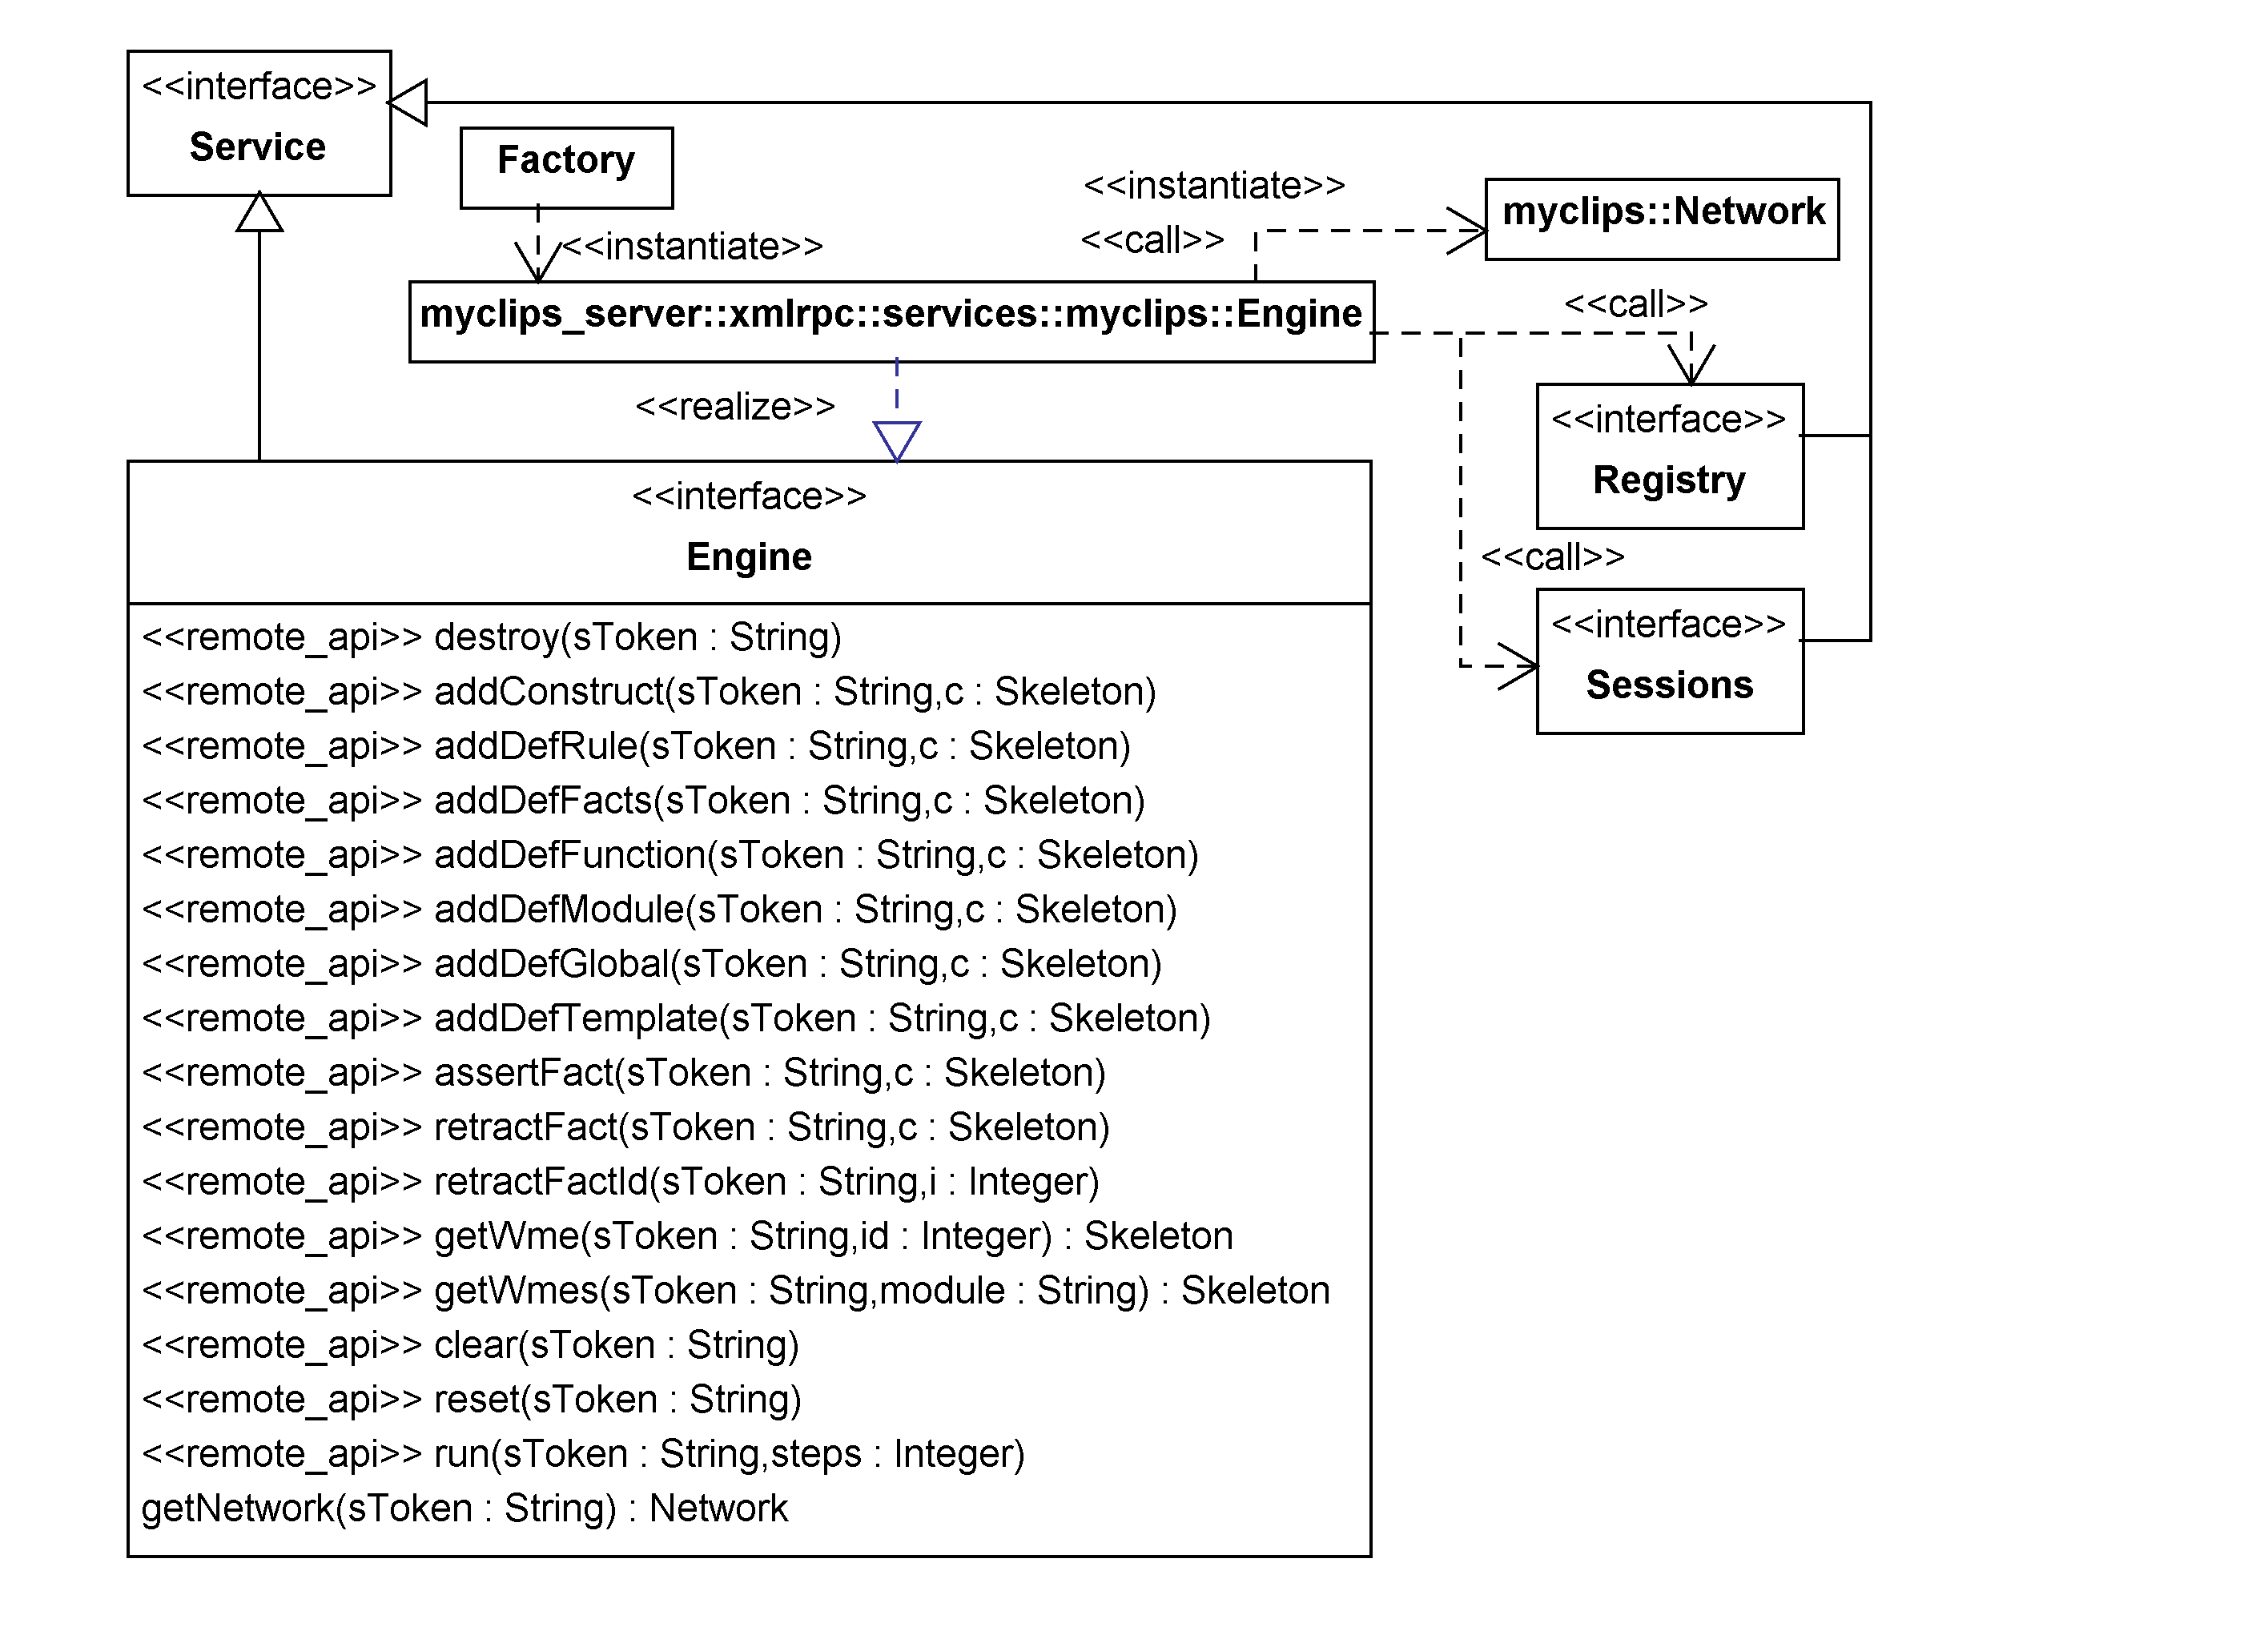
\includegraphics[width=1\textwidth]{Immagini/Capitolo3/Classi/myclips_server_services_Engine.png}
\caption{Package \emph{myclips\_server.xmlrpc.services}: vista delle classi e interfacce relative al servizio \emph{Engine}}\label{fig:class-myclips-server-services-engine}
\end{figure}

Il servizio che realizza il collegamento fra \emph{client} e il motore inferenziale prende il nome di \emph{Engine}~(\figurename~\ref{fig:class-myclips-server-services-engine}). Utilizzando i metodi pubblicizzati tramite l'interfaccia di servizio \emph{Engine}, al client viene data la possibilità di inizializzare il motore inferenziale aggiungendo costrutti (opportunamente creati tramite l'utilizzo del servizio \emph{Registry}), eseguire il ciclo \emph{recognize-act} e, utilizzando i metodi di ispezione forniti, analizzare lo stato finale del sistema. Tramite l'utilizzo dei servizi \emph{ClientIO} e \emph{ClientEvents}, il motore offre la stessa gamma di funzionalità utilizzabili attraverso un'istanza locale del sistema. La classe concreta che realizza il servizio si affida all'utilizzo dei metodi offerti dalla classe del core \emph{Network}.

\subsection{Terminale}

\begin{figure}[h]
\centering
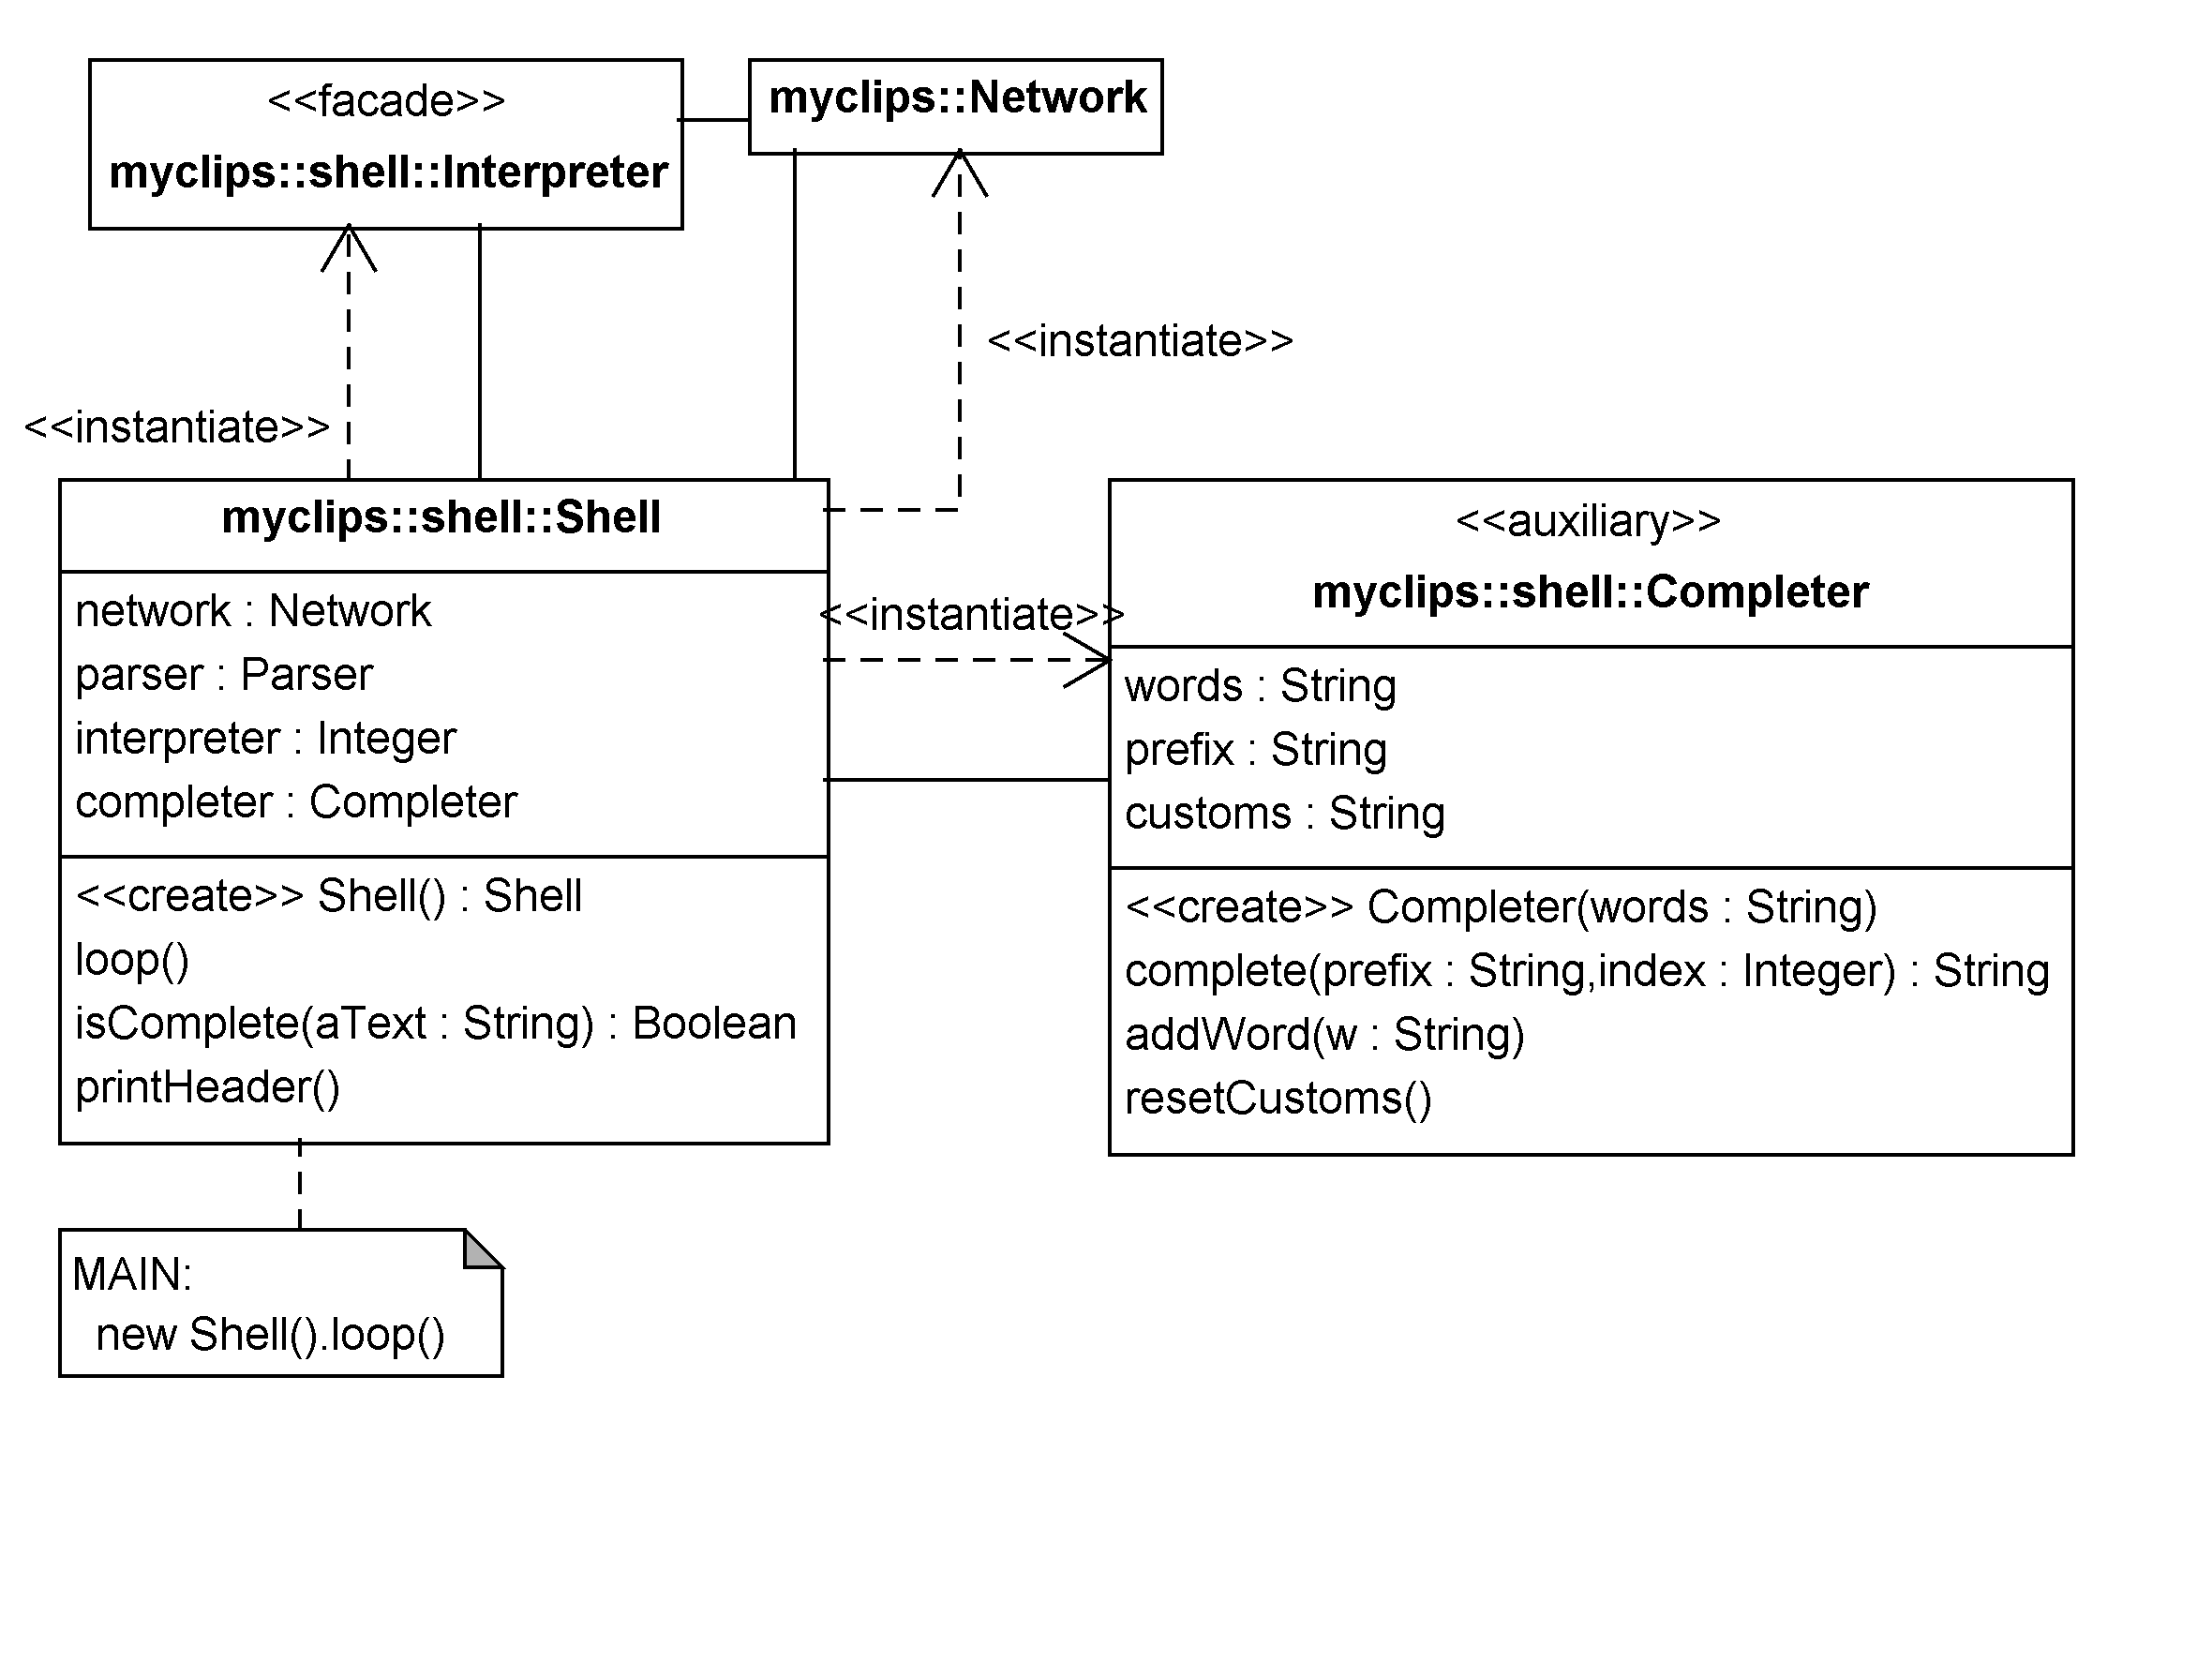
\includegraphics[width=1\textwidth]{Immagini/Capitolo3/Classi/myclips_shell_Shell.png}
\caption{Package \emph{myclips.shell}: vista delle classi relative al \emph{Terminale}}\label{fig:class-myclips-shell-Shell}
\end{figure}

L'interfaccia Terminale offerta dal sistema viene implementata tramite la collaborazione di due classi presenti nel \emph{package} \emph{myclips.shell}: \emph{Shell} e \emph{Completer}.~(\figurename~\ref{fig:class-myclips-shell-Shell})
La prima realizza il ciclo principale di immissione e valutazione dei comandi testuali forniti dall'utente, utilizzando le funzionalità di \emph{Interpreter}, la seconda valuta il completamento automatico delle immissioni dell'utente, quando richiesto dalla pressione di un tasto speciale.


\section{Implementazione}

La fase di implementazione ha richiesto la conversione delle strutture progettate e mostrate nei paragrafi precedenti tramite l'utilizzo di un linguaggio di programmazione. Inoltre è stata necessaria la selezione del protocollo da utilizzare per le comunicazioni \emph{client-server}.

\subsection{Tecnologie Utilizzate}

\subsubsection{Python}

\begin{figure}[h]
\centering
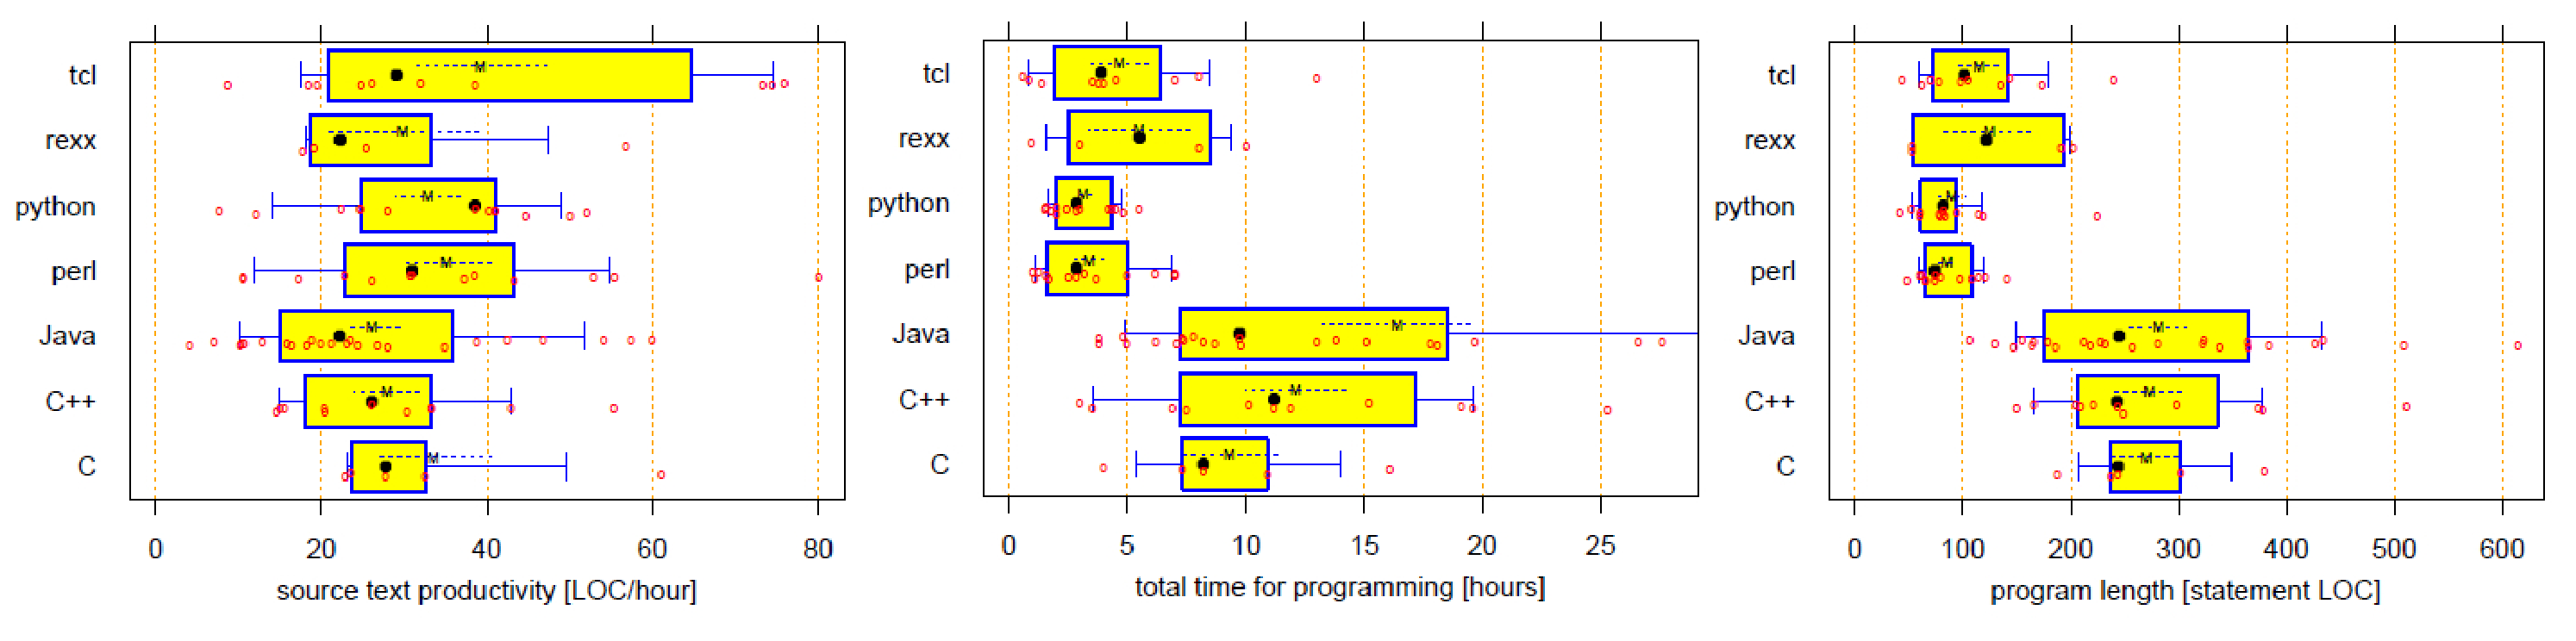
\includegraphics[viewport=0 0 1434 347, width=1\textwidth]{Immagini/Capitolo3/Python-comparison.pdf}
\caption[Comparazione fra Python e altri linguaggi di programmazione]{Comparazione fra Python e altri linguaggi di programmazione mostrando, da sinistra a destra, velocità di produzione del codice, tempo totale di produzione e lunghezza degli artefatti~\cite{prechelt2000}.}\label{fig:python-comparison}
\end{figure}

La scelta del linguaggio di programmazione da utilizzare per l'implementazione del sistema è ricaduta su linguaggio intepretato \emph{Python}\footnote{http://www.python.org/}. A supporto della scelta si propongono le seguenti argomentazioni:
\begin{description}
	\item[Gratuità:] Python è un linguaggio open-source utilizzabile, modificabile e distribuibile gratuitamente. Lo sviluppo del linguaggio è affidato ad una organizzazione \emph{no-profit} (Python Software Foundation)~\cite{pythonfaq}.
	
	\item[Facilità di sviluppo:] Python è un linguaggio di programmazione \emph{general-purpose} di alto livello. La grande varietà di librerie distribuite insieme alle implementazioni del linguaggio (con ambiti che variano dalla programmazione asincrona alla gestione degli archivi zip~\cite{pythonfaq}~\cite{pythonstdlib}) o prodotte dalla comunità\footnote{http://pypi.python.org/pypi} consente di utilizzare le soluzioni offerte per velocizzare i processi di sviluppo degli artefatti~\cite{prechelt2000}~\cite{prashant2008}.
	
	\item[Sinteticità del linguaggio:] studi comparativi fra linguaggi di programmazione attualmente disponibili (\figurename~\ref{fig:python-comparison}) hanno evidenziato la proprietà del linguaggio di utilizzare una sintassi concisa senza ridurre le capacità espressive~\cite{prechelt2000}~\cite{prashant2008}.
	
	\item[Meccanismi di riflessione:] il linguaggio integra dei meccanismi di riflessione e caricamento a \emph{run-time} avanzati che rendono agevole la realizzazione dei meccanismi di estensione dell'environment progettato. Le attività di inclusione di nuove funzioni di sistema o strategie CRS si riducono alla semplice serializzazione degli algoritmi, senza la necessità di eseguire fasi di compilazione o integrazione complesse.
	
	\item[Multi-piattaforma:] il supporto al linguaggio è disponibile per numerose piattaforme e sistemi operativi~\cite{pythonfaq} (compresi quelli richiesti per il  soddisfacimento del \emph{Vincolo-6}).
	
	\item[Capacità di integrazione:] sono disponibili numerose implementazioni di Python (con diversi livelli di compatibilità), realizzate in linguaggi come  Java\footnote{http://www.jython.org/}, C\#\footnote{http://ironpython.net/}, C\footnote{Implementazione di riferimento: http://www.python.org/}. Ognuna consente un'integrazione diretta con meccanismi propri del linguaggio di implementazione. In aggiunta, le capacità offerte dalle librerie permettono di utilizzare meccanismi di integrazione agnostici tra linguaggi eterogenei.
\end{description}

%Come rovescio della medaglia, la scelta ha determinato alcuni effetti sulle prestazioni complessive del sistema: nonostante le prestazioni teoricamente migliori ottenibili con linguaggi alternativi, il \emph{Vincolo-7} risulta egualmente soddisfatto. Le ridotte prestazioni offerte da Python (se messo in relazione con altri linguaggi), non sono state ritenute una ragione sufficiente ad invalidare la preferenza espressa, soprattutto tenendo conto dei vantaggi alternativi che la soluzione offre.

\subsubsection{Protocollo: XML-RPC}

\emph{Remote Procedure Call}, o \emph{RPC}, è un meccanismo tramite il quale un'applicazione posizionata su una \emph{macchina} richiede l'utilizzo di servizi forniti da un'altra applicazione residente su una \emph{macchina} differente. Con il termine \emph{macchina} non viene unicamente inteso un \emph{host}, un'installazione fisicamente separata, ma anche un processo residente in una porzione di memoria indipendente e che rende l'accesso alle risorse del servizio impossibile se non tramite il meccanismo \emph{RPC}. 

Il meccanismo \emph{RPC} prevede che una prima applicazione possa inviare uno o più messaggi ad una applicazione differente per invocare delle procedure. L'applicazione ricevente ha la possibilità,  a sua volta, di inviare i risultati dell'elaborazione tramite un ulteriore messaggio verso applicazione richiedente~\cite{MERRICK:2006:misc}.

\emph{RPC} descrive un meccanismo generalizzato per l'invocazione di procedure remote, non una concreta implementazione di un protocollo o di tecnologie per lo scambio dei messaggi fra gli \emph{host}. Partendo dal concetto generale di \emph{RPC}, nel tempo sono state proposte differenti implementazioni basate su protocolli proprietari o codifiche dei messaggi differenti~\cite{JAIRATH:2004:misc}~\cite{dcerpc}.

\begin{figure}[h]
\centering
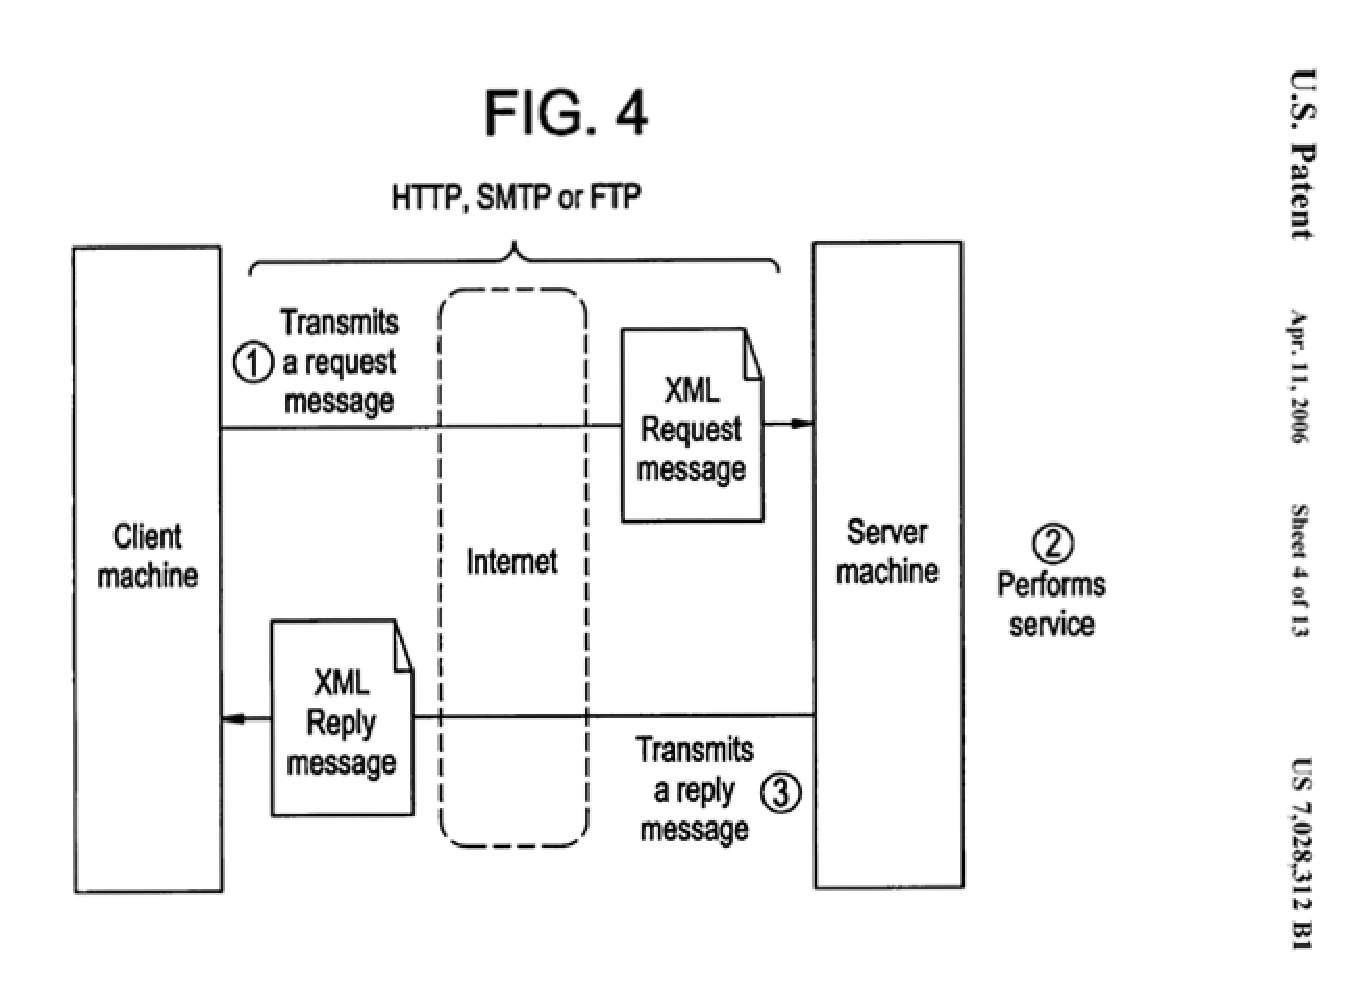
\includegraphics[scale=0.5, viewport=0 0 646 440]{Immagini/Capitolo3/XMLRPC-patent.pdf}
\caption[Comunicazione tramite \emph{XML-RPC}]{Comunicazione tramite \emph{XML-RPC}: immagine presente nella richiesta originale di brevetto~\cite{MERRICK:2006:misc}.}\label{fig:xmlrpc-patent}
\end{figure}

\emph{XML-RPC} è una fra le implementazioni proposte per \emph{RPC}: si propone come un meccanismo di chiamata a procedura remote semplice e versatile. Il brevetto originale con il quale è stato proposto descrive sia il meccanismo di chiamata, che un sistema per l'implementazione del metodo~\cite{MERRICK:2006:misc}.
\emph{XML-RPC} prevede lo scambio di richieste e risposte usando il formato \emph{XML}, attraverso meccanismi di trasporto multipli. Solitamente, con l'uso del termine \emph{XML-RPC} si è soliti però indicare il protocollo di scambio messaggi in \emph{XML} attraverso un meccanismo di trasporto basato sul protocollo \emph{HTTP}.

\begin{program}
\begin{verbatimtab}

POST /RPC2 HTTP/1.0
User-Agent: Frontier/5.1.2 (WinNT)
Host: betty.userland.com
Content-Type: text/xml
Content-length: 181


<?xml version="1.0"?>
<methodCall>
   <methodName>examples.getStateName</methodName>
   <params>
      <param>
         <value><i4>41</i4></value>
         </param>
      </params>
   </methodCall>
\end{verbatimtab}
\caption{Esempio di chiamata ad una procedura remota usando \emph{XML-RPC over HTTP}}\label{code:xmlrpc-request}
\end{program}

La codifica dei messaggi viene effettuata incapsulando i parametri di chiamata ed i valori di ritorno all'interno di appositi frammenti del documento \emph{XML}, i quali hanno il compito di attribuire una semantica alla stringa rappresentante il valore.

\begin{program}
\begin{verbatimtab}
HTTP/1.1 200 OK
Connection: close
Content-Length: 158
Content-Type: text/xml
Date: Fri, 17 Jul 1998 19:55:08 GMT
Server: UserLand Frontier/5.1.2-WinNT


<?xml version="1.0"?>
<methodResponse>
   <params>
      <param>
         <value><string>South Dakota</string></value>
         </param>
      </params>
   </methodResponse>
\end{verbatimtab}
\caption{Esempio di messaggi inviato a risposta di una chiamata a procedura remota usando \emph{XML-RPC over HTTP}}\label{code:xmlrpc-response}
\end{program}

I \emph{tag} che contengono il valore ne determinano il tipo. Nell'esempio fornito in Codice~\ref{code:xmlrpc-request}, il valore ''41'' (tipo \emph{integer}) viene incapsulato nel \emph{tag i4}. Il tag indica appunto che il tipo del valore, come da specifica, è un \emph{4 bytes signed integer}.

La specifica prevede la possibilità di utilizzare un set di tipi atomici con i quali rappresentare tutti i parametri di chiamata a procedura o i valori di ritorno (''integer'', ''string'', ''boolean'', ''double'', ''dateTime.iso8601'', ''base64'') e un gruppo di strutture composte (''struct'' per strutture analoghe a dizionari, ''array'' per vettori)~\cite{xmlrpcspec}.

A supporto della scelta di utilizzare \emph{XML-RPC} come protocollo RPC si propongono le seguenti argomentazioni:
\begin{description}
	\item[Semplicità:] il protocollo formalizza un metodo di interazione relativamente semplice se comparato con le alternative disponibili. Il trasferimento delle informazioni avviene nella forma di parametri di input o output di funzioni ed il modello di comunicazione non forza l'utilizzo di modelli di sicurezza complessi. La fornitura del servizio non richiede la necessità di creare descrizioni formali dello stesso, sebbene l'utilizzo di strumenti di supporto\footnote{XRDL: http://code.google.com/p/xrdl/} permettano la generazione automatica di client per i servizi.
	\item[Disponibilità:] l'utilizzo del protocollo è possibile in molti linguaggi di programmazione e piattaforme attraverso le implementazioni fornite da librerie apposite. Una stima approssimativa suggerisce la disponibilità di oltre 40 implementazioni differenti per un totale di oltre 25 piattaforme e linguaggi di programmazione~\cite{wikipedia-xmlrpc}.
\end{description}

\subsubsection{Pyparsing}
Pyparsing\footnote{http://pyparsing.wikispaces.com/home}$^,$\footnote{http://sourceforge.net/projects/pyparsing} è un modulo completamente scritto in linguaggio Python che fornisce un insieme di classi per la creazione di parser di espressioni, sia elementari che complesse e che prevedono l'uso di componenti variabili. Le espressioni sono combinate usando gruppi di operatori (come ad esempio ''+'' per definire la sequenzialità o ''$\mid$'' per le alternative), prevedendo l'utilizzo di espressioni replicate o ricorsive~\cite{pyparsing-gs}.

\begin{figure}[h]
\centering
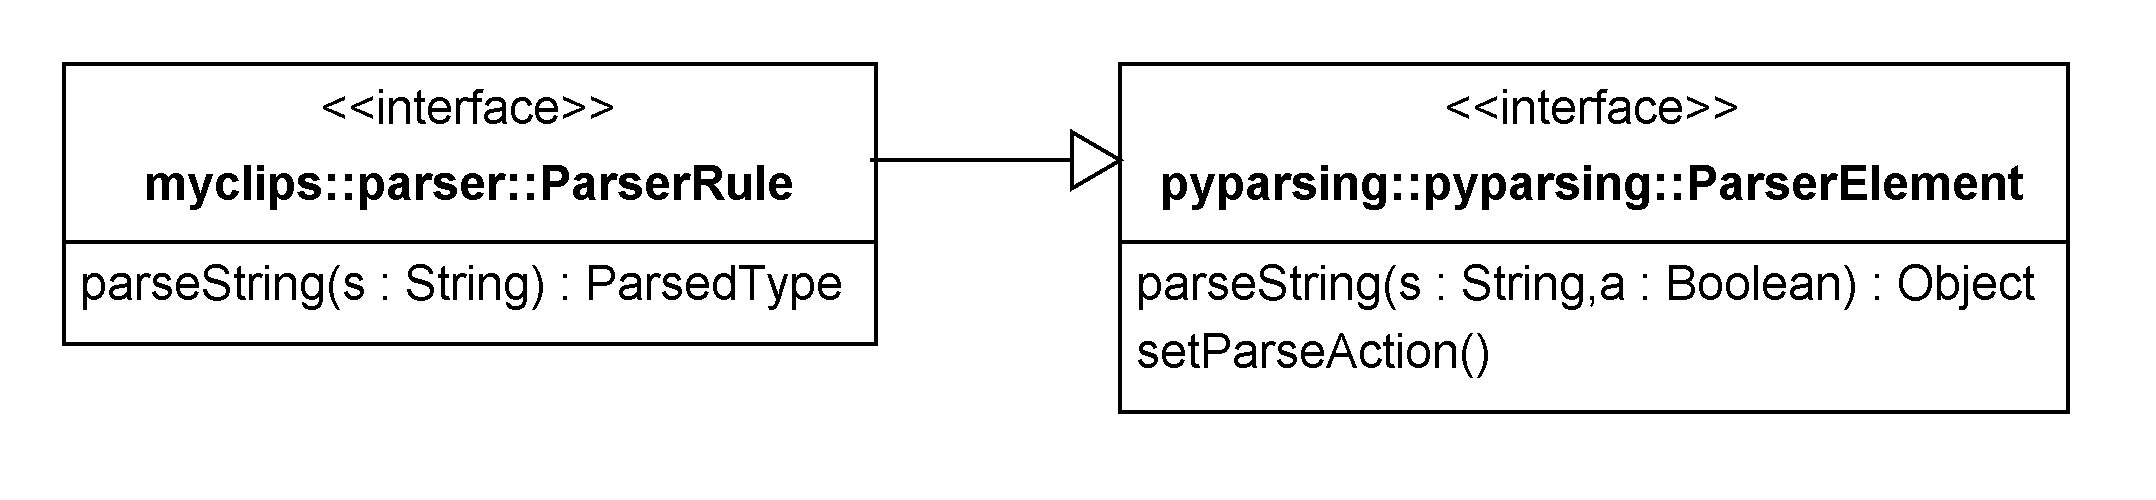
\includegraphics[width=1\textwidth]{Immagini/Capitolo3/Classi/myclips_parser_PyParsing.png}
\caption[Integrazione di PyParsing nel modulo Parser]{Integrazione di PyParsing nel modulo Parser}\label{fig:class-myclips-parser-pyparsing}
\end{figure}

Il modulo Parser è stato implementato facendo uso delle classi fornite da Pyparsing per la definizione delle regole di valutazione. L'interfaccia \emph{ParserRule} mostrata nella descrizione del modulo Parser è stata sostituita dall'uso delle classi fornite da PyParsing. La classe principale \emph{Parser} è stata conseguentemente adattata per l'uso delle nuove istanze (\figurename~\ref{fig:class-myclips-parser-pyparsing})~\cite{pyparsing-apidoc}.

\subsubsection{BList}

\begin{figure}[h]
\centering
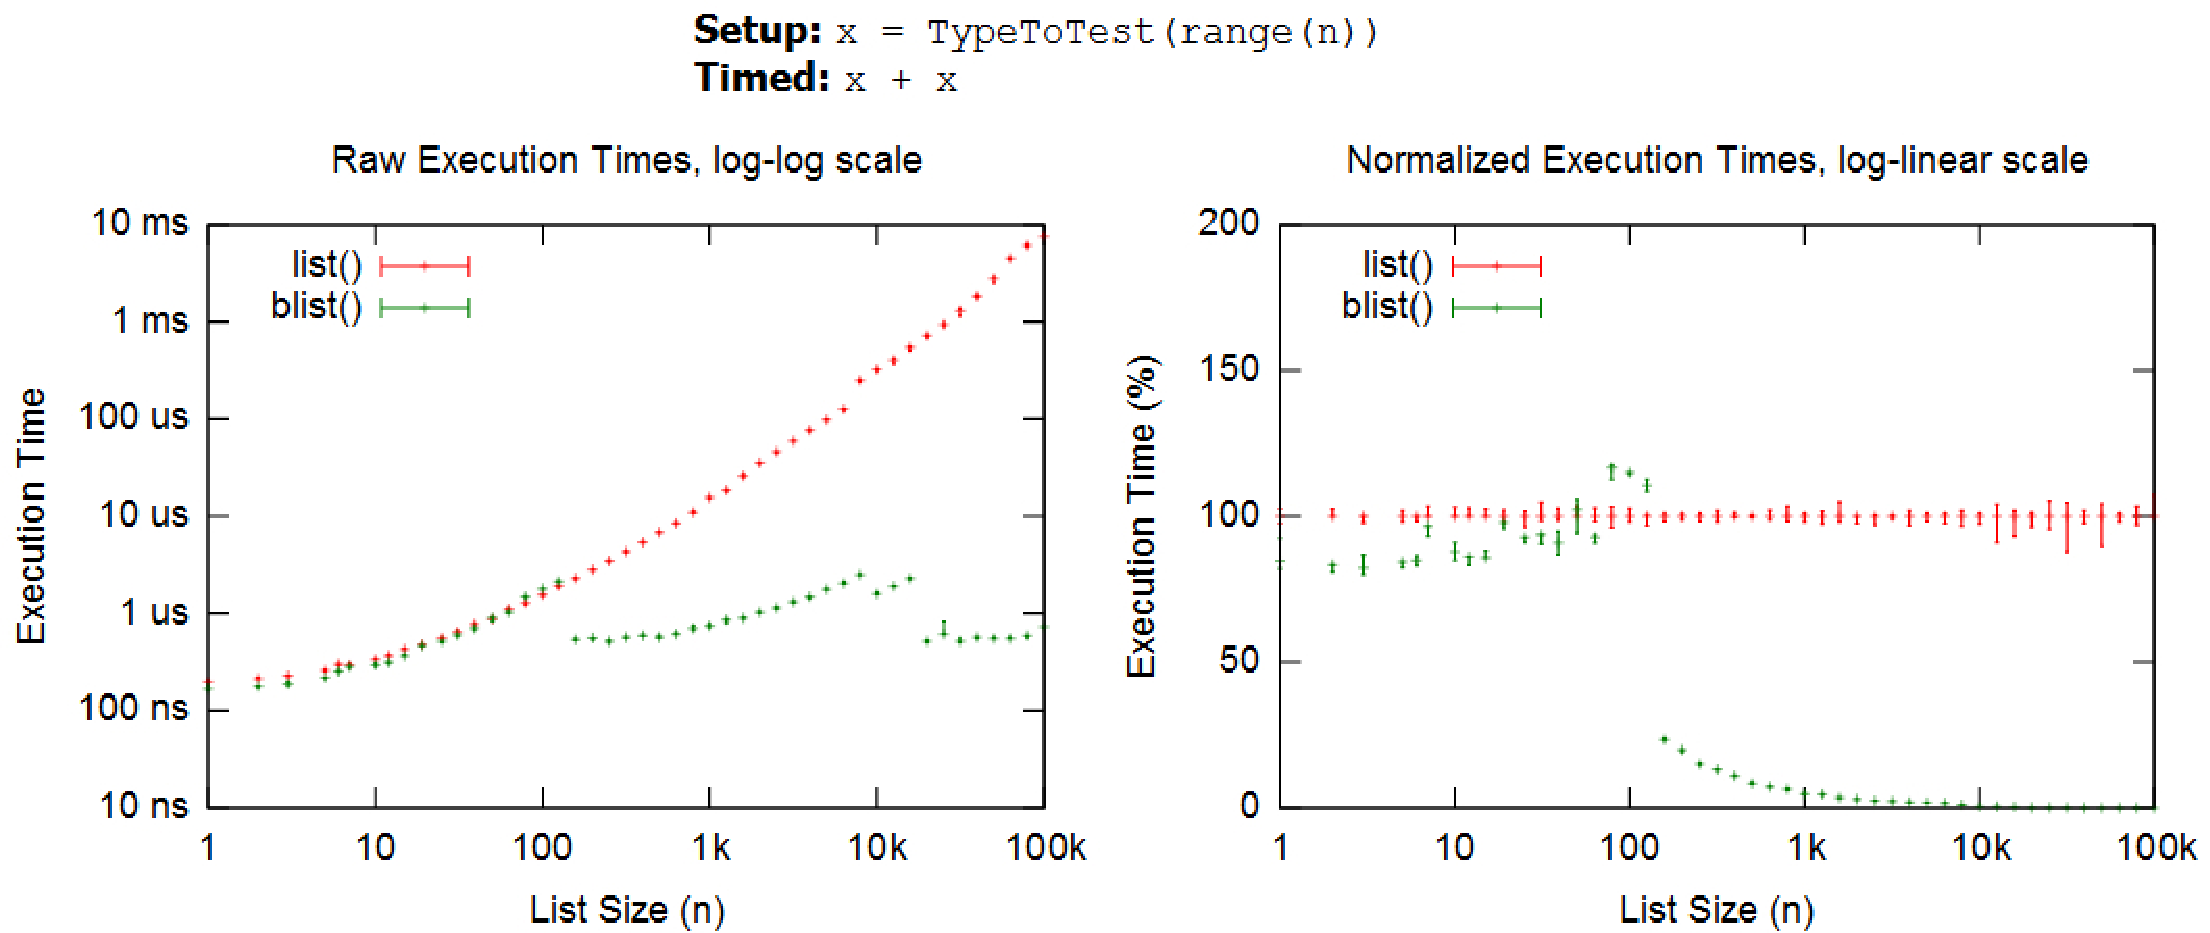
\includegraphics[width=1\textwidth]{Immagini/Capitolo3/BList-comparison.pdf}
\caption[Confronto fra l'implementazione di vettori fornita da BList e di \emph{default}]{Confronto fra l'implementazione di vettori fornita da BList e quella di \emph{default} fornita da CPython: prestazioni dell'operazione di inserimento~\cite{blist-prest}.}\label{fig:blist-comparison}
\end{figure}

La libreria BList\footnote{http://stutzbachenterprises.com/blist/} è un modulo Python per la sostituzione trasparente dell'implementazione delle collezioni fornite dal linguaggio~\cite{blist-manual}. Fornisce prestazioni superiori rispetto all'implementazione \emph{standard} dei vettori durante la manipolazione di collezioni di grandi dimensioni e fornisce realizzazioni di liste ordinate (\figurename~\ref{fig:blist-comparison})~\cite{blist-prest}.

Le liste ordinate fornite da Blist sono state utilizzate nell'implementazione delle strategie CRS \emph{Mea} e \emph{Lex} per l'inserimento ordinato delle attivazioni nell'agenda.


\subsubsection{NetworkX}

\begin{figure}
\centering
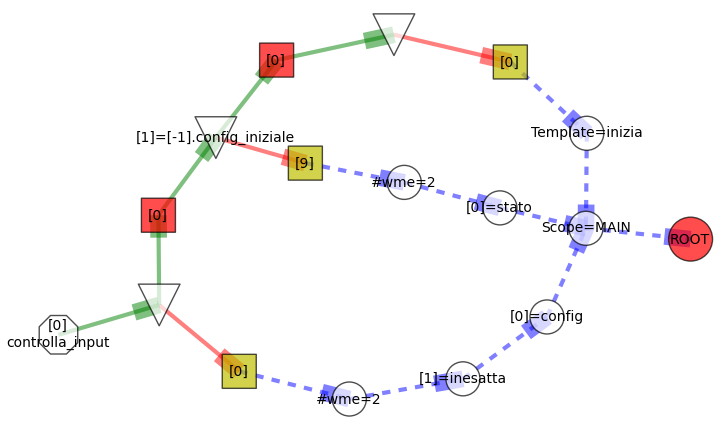
\includegraphics[width=1\textwidth]{Immagini/Capitolo3/draw-circuit.png}
\caption[Esempio d'uso della libreria NetworkX]{Esempio d'uso della libreria NetworkX per la rappresentazione del circuito compilato ottenuto dalla regola \emph{controlla\_input} in Codice~\ref{code:agricoltore-1}}\label{fig:networkx-example}
\end{figure}

NetworkX\footnote{http://networkx.lanl.gov/} è un pacchetto software per il linguaggio Python per la creazione, manipolazione e lo studio di strutture, dinamiche e funzioni di reti complesse.

La libreria viene utilizzata per l'implementazione del \emph{Listener} \emph{NetworkPlotter}, usato per offrire una rappresentazione grafica della RETE compilata (\figurename~\ref{fig:networkx-example}), e per la generazione degli script in formato \emph{dot}\footnote{http://en.wikipedia.org/wiki/DOT\_language} contenenti una serializzazione della rappresentazione di RETE da trasmettere ai \emph{client}.

\subsection{Specifica delle classi \emph{Core}}

L'implementazione delle funzionalità previste dal componente Core del sistema è stata suddivisa in sette \emph{package} differenti:

\begin{enumerate}
	\item \texttt{myclips}: package di base che organizza le classi concrete e astratte d'utilità condivise da altri package
	\item \texttt{myclips.parser}: sono organizzate al suo interno le classi relative alla valutazione del linguaggio di specifica e alle classi d'entità utilizzate per mappare i costrutti del linguaggio di specifica
	\item \texttt{myclips.listener}: contiene le classi \emph{listener} per il monitoraggio degli eventi e l'implementazione dei comportamenti associati
	\item \texttt{myclips.functions}: racchiude definizioni e implementazioni delle funzioni di sistema utilizzate nell\emph{environment}
	\item \texttt{myclips.rete}: contiene le classi relative all'implementazione dell'algoritmo RETE per il \emph{matching}. Le classi sono strutturate ulteriormente in 3 \emph{sub-package}:
		\begin{enumerate}
			\item \texttt{myclips.rete}: contiene le classi astratte per la formalizzazione delle interfacce dei nodi e delle memorie
			\item \texttt{mycllps.rete.nodes}: organizza le classi relative alle implementazioni dei nodi del grafo di RETE
			\item \texttt{myclips.rete.tests}: organizza le interfacce e le realizzazioni delle classi di test utilizzate nei nodi
		\end{enumerate}
	\item \texttt{myclips.strategies}: organizza le interfacce e le classi relative alla gestione delle strategie di risoluzione dei conflitti, cosi come le realizzazioni delle strategie fornite dal sistema
	\item \texttt{myclips.shell}: racchiude le classi relative alle funzionalità svolte dalla componente \emph{Interpreter}
\end{enumerate}

Di seguito si fornisce il dettaglio delle classi, organizzate in base al \emph{package} di appartenenza

\subsubsection{Package \texttt{myclips}}

\begin{longtable}{p{5.5cm}p{6.5cm}}
\hline 
\textbf{Classe} & \textbf{Descrizione} \\ 
\hline\hline 
\endhead

\multicolumn{2}{c}{\emph{Modulo} \texttt{Agenda.py}}\\
	\hdashline[5pt/5pt]
		\texttt{Agenda} & Organizza le strutture di memorizzazione delle attivazioni fornite dalle strategie CRS e le strategie stesse\\ 
	\hdashline[1pt/5pt]
		\texttt{AgendaNoMoreActi\-vationError} & Eccezione utilizzata l'assenza di ulteriori attivazioni per il focusStack selezionato\\ 
	\hline\\

\multicolumn{2}{c}{\emph{Modulo} \texttt{EventsManager.py}}\\
	\hdashline[5pt/5pt]
		\texttt{EventsManager} & Gestore degli eventi e dei listener\\ 
	\hline\\

\multicolumn{2}{c}{\emph{Modulo} \texttt{Fact.py}}\\
	\hdashline[5pt/5pt]
		\texttt{Fact} & Rappresenta un fatto\\ 
	\hdashline[1pt/5pt]
		\texttt{Fact\-Length\-Not\-Computable\-Error} & Eccezione utilizzata per notificare l'impossibilità di computare la lunghezza delle componenti di un'istanza \\ 
	\hdashline[1pt/5pt]
		\texttt{Fact\-Slot\-Value\-Can\-not\-Be\-Set\-Er\-ror} & Eccezione utilizzata per notificare l'errore relativo al tentativo di modificare lo slot di un fatto non di tipo \emph{TemplateFact}\\ 
	\hdashline[1pt/5pt]
		\texttt{Fact\-Slots\-Not\-Com\-pu\-ta\-ble\-Error} & Eccezione utilizzata per notificare l'impossibilità di valutare l'insieme degli slot\\
	\hdashline[1pt/5pt]
		\texttt{Fact\-InvalidIndex} & Eccezione utilizzata per notificare l'errore nella richiesta di un indice non valido per un \emph{OrderedFact}\\ 
	\hdashline[1pt/5pt]
		\texttt{Fact\-InvalidSlotName} & Eccezione utilizzata per notificare l'errore nella richiesta di uno slot non valido per un \emph{TemplateFact}\\ 
	\hline\\

\multicolumn{2}{c}{\emph{Modulo} \texttt{FunctionsManager.py}}\\
	\hdashline[5pt/5pt]
		\texttt{FunctionsManager} & Manager delle definizioni di funzione utilizzabili in uno \emph{Scope}\\ 
	\hdashline[1pt/5pt]
		\texttt{FunctionDefinition} & Rappresenta una definizione di funzione\\ 
	\hdashline[1pt/5pt]
		\texttt{FunctionConstraint} & Rappresenta una restrizione definita nella firma di funzione\\ 
	\hdashline[1pt/5pt]
		\texttt{Contraint\_MinArgsLength} & Definisce una restrizione sul numero minimo di parametri richiesti dalla chiamata a funzione\\ 
	\hdashline[1pt/5pt]
		\texttt{Contraint\_MaxArgsLength} & Definisce una restrizione sul numero massimo di parametri richiesti dalla chiamata a funzione\\ 
	\hdashline[1pt/5pt]
		\texttt{Contraint\_ExactArgsLength} & Definisce una restrizione sull'esatto numero di parametri richiesti dalla chiamata a funzione\\ 
	\hdashline[1pt/5pt]
		\texttt{Contraint\_ArgType} & Definisce una restrizione sul un tipo di un parametro richiesto dalla chiamata a funzione\\ 
	\hline\\

\multicolumn{2}{c}{\emph{Modulo} \texttt{GlobalsManager.py}}\\
	\hdashline[5pt/5pt]
		\texttt{GlobalsManager} & Manager delle definizioni di variabili globali utilizzabili in uno \emph{Scope}\\ 
	\hdashline[1pt/5pt]
		\texttt{GlobalVarDefinition} & Rappresenta una definizione di variabile globale\\ 
	\hline\\

\multicolumn{2}{c}{\emph{Modulo} \texttt{ModulesManager.py}}\\
	\hdashline[5pt/5pt]
		\texttt{ModulesManager} & Manager degli \emph{Scope} definiti\\ 
	\hdashline[1pt/5pt]
		\texttt{Modules\-Manager\-Re\-de\-fi\-ni\-tion\-Er\-ror} & Eccezione usata per notificare il tentativo di ridefinire un modulo già definito\\ 
	\hdashline[1pt/5pt]
		\texttt{UnknownModulesError} & Eccezione usata per notificare il tentativo di sostituire lo \emph{Scope} corrente con uno non definito\\ 
	\hline\\

\multicolumn{2}{c}{\emph{Modulo} \texttt{MyClipsException.py}}\\
	\hdashline[5pt/5pt]
		\texttt{MyClipsException} & Classe base di tutte le eccezioni propagate in MyCLIPS\\ 
	\hdashline[1pt/5pt]
		\texttt{MyClipsBugException} & Classe utilizzata per notificare una condizione errata del sistema dovuta a errori di implementazione\\ 
	\hline\\

\multicolumn{2}{c}{\emph{Modulo} \texttt{Observable.py}}\\
	\hdashline[5pt/5pt]
		\texttt{Observable} & Classe astratta per la realizzazione della componente \emph{Observable} del design pattern \emph{Observer}\\ 
	\hline\\


\multicolumn{2}{c}{\emph{Modulo} \texttt{Observer.py}}\\
	\hdashline[5pt/5pt]
		\texttt{Observer} & Classe astratta per la realizzazione della componente \emph{Observer} del design pattern \emph{Observer}\\ 
	\hline\\

\multicolumn{2}{c}{\emph{Modulo} \texttt{RestrictedManager.py}}\\
	\hdashline[5pt/5pt]
		\texttt{RestrictedManager} & Classe astratta che generalizza la gestione delle definizioni sottoposte a vincoli di \emph{Scope}\\ 
	\hdashline[1pt/5pt]
		\texttt{RestrictedDefinition} & Classe astratta che generalizza le definizioni gestibili da \emph{RestrictedManager}\\ 
	\hdashline[1pt/5pt]
		\texttt{MultipleDefinitionError} & Eccezione utilizzata per notificare il tentativo di ridefinire un elemento già esplicitato\\ 
	\hline\\

\multicolumn{2}{c}{\emph{Modulo} \texttt{Scope.py}}\\
	\hdashline[5pt/5pt]
		\texttt{Scope} & Rappresenta una definizione di modulo e gestisce i manager delle definizioni disponibili nel modulo\\ 
	\hdashline[1pt/5pt]
		\texttt{ScopeImport} & Rappresenta una direttiva di importazione\\ 
	\hdashline[1pt/5pt]
		\texttt{ScopeExport} & Rappresenta una definizione di esportazione\\ 
	\hdashline[1pt/5pt]
		\texttt{\_ScopeExportPromise} & Rappresenta una definizione di promessa di esportazione\\ 
	\hdashline[1pt/5pt]
		\texttt{ScopeDefinitionNotFound} & Eccezione utilizzata per notificare il tentativo di accedere ad uno \emph{Scope} non definito\\ 
	\hdashline[1pt/5pt]
		\texttt{ScopeDefinitionConflict} & Eccezione utilizzata per notificare un conflitto di definizioni importante o esportate\\ 
	\hline\\

\multicolumn{2}{c}{\emph{Modulo} \texttt{Settings.py}}\\
	\hdashline[5pt/5pt]
		\texttt{Settings} & Gestisce le impostazioni di sessione del motore inferenziale\\ 
	\hline\\

\multicolumn{2}{c}{\emph{Modulo} \texttt{TemplatesManager.py}}\\
	\hdashline[5pt/5pt]
		\texttt{TemplatesManager} & Manager delle definizioni di template utilizzabili in uno \emph{Scope}\\ 
	\hdashline[1pt/5pt]
		\texttt{TemplateDefinition} & Rappresenta una definizione di template\\ 
	\hdashline[1pt/5pt]
		\texttt{SlotDefinition} & Rappresenta una definizione di slot di template\\ 
	\hdashline[1pt/5pt]
		\texttt{Attribute} & Generalizzazione di un attributo associabile ad una definizione di slot di template\\ 
	\hdashline[1pt/5pt]
		\texttt{Attribute\_DefaultValue} & Rappresenta la definizione del valore di default associato ad uno slot di template\\ 
	\hdashline[1pt/5pt]
		\texttt{Attribute\_TypeConstraint} & Rappresenta la definizione di restrizione di tipo associata ad uno slot di template\\ 
	\hline\\

\end{longtable} 


\subsubsection{Package \texttt{myclips.parser}}

\begin{longtable}{p{5.5cm}p{6.5cm}}
\hline 
\textbf{Classe} & \textbf{Descrizione} \\ 
\hline\hline 
\endhead

\multicolumn{2}{c}{\emph{Modulo} \texttt{Parser.py}}\\
	\hdashline[5pt/5pt]
		\texttt{Parser} & Organizza e gestisce le regole di \emph{parsing} del linguaggio di definizione e esegue la conversione in istanze utilizzabili nel motore inferenziale \\ 
	\hline\\

\multicolumn{2}{c}{\emph{Modulo} \texttt{Types.py}}\\
	\hdashline[5pt/5pt]
		\texttt{ParsedType} & Classe base per le entità riconosciute tramite \emph{Parser}\\ 
	\hdashline[1pt/5pt]
		\texttt{BaseParsedType} & Classe base per i tipi atomici\\ 
	\hdashline[1pt/5pt]
		\texttt{HasScope} & Classe astratta per le entità che richiedono uno \emph{Scope} per validare o aggiungere una definizione\\ 
	\hdashline[1pt/5pt]
		\texttt{Number} & Classe base per i tipi numerici\\ 
	\hdashline[1pt/5pt]
		\texttt{Lexeme} & Classe base per i tipi simbolici\\
	\hdashline[1pt/5pt]
		\texttt{Integer} & Mappa un elemento Integer\\
	\hdashline[1pt/5pt]
		\texttt{Float} & Mappa un element Float\\ 
	\hdashline[1pt/5pt]
		\texttt{Symbol} & Mappa un elemento Symbol\\ 
	\hdashline[1pt/5pt]
		\texttt{String} & Mappa una stringa compresa fra doppi apici\\ 
	\hdashline[1pt/5pt]
		\texttt{Variable} & Classe base per le entità variabili\\ 	
	\hdashline[1pt/5pt]
		\texttt{SingleFieldVariable} & Mappa una variabile di tipo \emph{single-field}\\ 
	\hdashline[1pt/5pt]
		\texttt{MultiFieldVariable} & Mappa una variabile di tipo \emph{multi-field}\\ 
	\hdashline[1pt/5pt]
		\texttt{UnnamedSingleFieldVariable} & Mappa un wildcard \emph{single-field}\\
	\hdashline[1pt/5pt]
		\texttt{UnnamedMultiFieldVariable} & Mappa un wildcard \emph{multi-field}\\ 
	\hdashline[1pt/5pt]
		\texttt{GlobalVariable} & Mappa una variable globale\\ 
	\hdashline[1pt/5pt]
		\texttt{FunctionCall} & Mappa una chiamata a funzione\\
	\hdashline[1pt/5pt]
		\texttt{DefFactsConstruct} & Mappa un costrutto \emph{deffacts}\\
	\hdashline[1pt/5pt]
		\texttt{OrderedRhsPattern} & Mappa una definizione di fatto in notazione \emph{Ordered-Fact}\\ 
	\hdashline[1pt/5pt]
		\texttt{TemplateRhsPattern} & Mappa una definizione di fatto in notazione \emph{Template-Fact}\\ 
	\hdashline[1pt/5pt]
		\texttt{FieldRhsSlot} & Classe astratta per la definizione di un valore di uno slot di un fatto in notazione \emph{Template-Fact} \\ 
	\hdashline[1pt/5pt]
		\texttt{MultiFieldRhsSlot} & Mappa un valore \emph{multi-field} in uno slot di un fatto in notazione \emph{Template-Fact} \\ 
	\hdashline[1pt/5pt]
		\texttt{SingleFieldRhsSlot} & Mappa un valore \emph{single-field} in uno slot di un fatto in notazione \emph{Template-Fact} \\ 
	\hdashline[1pt/5pt]
		\texttt{DefRuleConstruct} & Mappa un costrutto \emph{defrule}\\ 
	\hdashline[1pt/5pt]
		\texttt{RuleProperty} & Mappa una definizione di proprietà di una regola\\
	\hdashline[1pt/5pt]
		\texttt{PatternCE} & Classe base per i \emph{PatternCE}\\
	\hdashline[1pt/5pt]
		\texttt{OrderedPatternCE} & Mappa una definizione di pattern per il ritrovamento di un \emph{Ordered-Fact}\\ 
	\hdashline[1pt/5pt]
		\texttt{TemplatePatternCE} & Mappa una definizione di pattern per il ritrovamento di un \emph{Template-Fact}\\ 
	\hdashline[1pt/5pt]
		\texttt{AssignedPatternCE} & Mappa una definizione di pattern associato a variabile\\ 
	\hdashline[1pt/5pt]
		\texttt{NotPatternCE} & Mappa una definizione di pattern negata\\ 
	\hdashline[1pt/5pt]
		\texttt{ExistsPatternCE} & Mappa una definizione di pattern \emph{exists-CE}\\ 
	\hdashline[1pt/5pt]
		\texttt{AndPatternCE} & Mappa una definizione di congiunzione di pattern\\ 
	\hdashline[1pt/5pt]
		\texttt{OrPatternCE} & Mappa una definizione di pattern \emph{or-CE}\\ 
	\hdashline[1pt/5pt]
		\texttt{TestPatternCE} & Mappa una definizione di pattern \emph{test-CE}\\
	\hdashline[1pt/5pt]
		\texttt{Constraint} & Mappa una definizione di condizione in un pattern\\ 
	\hdashline[1pt/5pt]
		\texttt{ConnectedConstraint} & Mappa una definizione di condizione collegata in un pattern\\ 
	\hdashline[1pt/5pt]
		\texttt{Term} & Classe astratta per i termini di un pattern\\ 
	\hdashline[1pt/5pt]
		\texttt{NotTerm} & Mappa un termine negato di un pattern\\ 
	\hdashline[1pt/5pt]
		\texttt{PositiveTerm} & Mappa un termine di un pattern\\ 
	\hdashline[1pt/5pt]
		\texttt{FieldLhsSlot} & Classe astratta per la definizione di slot per i pattern per fatti \emph{Template-Fact}\\ 
	\hdashline[1pt/5pt]
		\texttt{SingleFieldLhsSlot} & Mappa una definizione di slot \emph{single-field} in un pattern \emph{TemplatePatternCE}\\ 
	\hdashline[1pt/5pt]
		\texttt{MultiFieldLhsSlot} & Mappa una definizione di slot \emph{multi-field} in un pattern \emph{TemplatePatternCE}\\ 
	\hdashline[1pt/5pt]
		\texttt{SlotDefinition} & Classe base per le definizioni di slot nei costrutti \emph{deftemplate}\\ 
	\hdashline[1pt/5pt]
		\texttt{SingleSlotDefinition} & Mappa una definizione di slot singolo\\ 
	\hdashline[1pt/5pt]
		\texttt{MultiSlotDefinition} & Mappa una definizione di slot multiplo\\ 
	\hdashline[1pt/5pt]
		\texttt{Attribute} & Classe base per le definizioni di attributi di slot\\ 
	\hdashline[1pt/5pt]
		\texttt{DefaultAttribute} & Mappa una definizione di attributo di tipo default per uno slot\\ 
	\hdashline[1pt/5pt]
		\texttt{TypeAttribute} & Mappa una definizione di attributo per restrizione di tipo per uno slot\\ 
	\hdashline[1pt/5pt]
		\texttt{DefTemplateConstruct} & Mappa un costrutto \emph{deftemplate}\\ 
	\hdashline[1pt/5pt]
		\texttt{DefGlobalConstruct} & Mappa un costrutto \emph{defglobal}\\ 
	\hdashline[1pt/5pt]
		\texttt{GlobalAssignment} & Mappa un'assegnazione di valore ad una variabile globale\\ 
	\hdashline[1pt/5pt]
		\texttt{PortItem} & Mappa una definizione di elemento importabile o esportabile\\ 
	\hdashline[1pt/5pt]
		\texttt{ImportSpecification} & Mappa una definizione di specifica di importazione di costrutti per un modulo\\ 
	\hdashline[1pt/5pt]
		\texttt{ExportSpecification} & Mappa una definizione di specifica di esportazione di costrutti per un modulo\\ 
	\hdashline[1pt/5pt]
		\texttt{DefModuleConstruct} & Mappa un costrutto \emph{defmodule}\\ 
	\hdashline[1pt/5pt]
		\texttt{DefFunctionConstruct} & Mappa un costrutto \emph{deffunction}\\ 
	\hdashline[1pt/5pt]
		\texttt{TypeInstanceCreationError} & Eccezione usata per indicare l'impossibilità di creazione di un'istanza definizione\\ 
	\hdashline[1pt/5pt]
		\texttt{Type\-Recoverable\-Instance\-Creation\-Error} & Eccezione usata per indicare un errore recuperabile nella creazione di un'istanza di definizione\\ 
	\hline\\

\end{longtable}


\subsubsection{Package \texttt{myclips.listeners}}

\begin{longtable}{p{5.5cm}p{6.5cm}}
\hline 
\textbf{Classe} & \textbf{Descrizione} \\ 
\hline\hline 
\endhead

\multicolumn{2}{c}{\emph{Modulo} \texttt{EventsManagerListener.py}}\\
	\hdashline[5pt/5pt]
		\texttt{EventsManagerListener} & Classe astratta per la definizione dell'interfaccia richiesta ai listener utilizzabili con \emph{EventsManager} \\ 
	\hline\\

\multicolumn{2}{c}{\emph{Modulo} \texttt{ActionWatcher.py}}\\
	\hdashline[5pt/5pt]
		\texttt{ActionWatcher} & Controlla il realizzarsi di eventi legati all'esecuzione di azioni \\ 
	\hline\\

\multicolumn{2}{c}{\emph{Modulo} \texttt{ActivationsWatcher.py}}\\
	\hdashline[5pt/5pt]
		\texttt{ActivationsWatcher} & Controlla il realizzarsi di eventi legati all'aggiunta o rimozione di attivazioni nel \emph{conflict-set} \\ 
	\hline\\

\multicolumn{2}{c}{\emph{Modulo} \texttt{FactsWatcher.py}}\\
	\hdashline[5pt/5pt]
		\texttt{FactsWatcher} & Controlla il realizzarsi di eventi legati all'asserzione o ritrattazione di fatti nella \emph{working-memory} \\ 
	\hline\\

\multicolumn{2}{c}{\emph{Modulo} \texttt{FocusWatcher.py}}\\
	\hdashline[5pt/5pt]
		\texttt{FocusWatcher} & Controlla il realizzarsi di eventi legati al cambiamento del focus \\ 
	\hline\\

\multicolumn{2}{c}{\emph{Modulo} \texttt{RulesWatcher.py}}\\
	\hdashline[5pt/5pt]
		\texttt{RulesWatcher} & Controlla il realizzarsi di eventi legati all'esecuzione di regole \\ 
	\hline\\
	
\multicolumn{2}{c}{\emph{Modulo} \texttt{StrategyWatcher.py}}\\
	\hdashline[5pt/5pt]
		\texttt{StrategyWatcher} & Controlla il realizzarsi di eventi legati al cambiamento della strategia di risoluzione dei conflitti \\ 
	\hline\\

\multicolumn{2}{c}{\emph{Modulo} \texttt{\_\_init\_\_.py}}\\
	\hdashline[5pt/5pt]
		\texttt{NetworkPlotter} & Controlla il realizzarsi di eventi legati alla costruzione del \emph{network} e li inoltra ad un adattatore per la visualizzazione grafica\\ 
	\hline\\

\multicolumn{2}{c}{\emph{Modulo} \texttt{\_NetworkPlotterAdapter\_NetworkX.py}}\\
	\hdashline[5pt/5pt]
		\texttt{\_NetworkPlotterAdapter\_NetworkX} & Inoltra gli eventi di costruzione del \emph{network} alla libreria \emph{NetworkX} per la generazione del grafo\\ 
	\hdashline[1pt/5pt]
		\texttt{\_NetworkXWrapper} & Incapsula l'interfaccia della libreria \emph{NetworkX} in una utilizzabile da \emph{\_NetworkPlotterAdapter\_NetworkX}\\ 
	\hline\\

\multicolumn{2}{c}{\emph{Modulo} \texttt{NetworkBuildPrinter.py}}\\
	\hdashline[5pt/5pt]
		\texttt{NetworkBuildPrinter} & Controlla il realizzarsi di eventi legati alla costruzione del \emph{network} e li visualizza su console \emph{stdout} \\ 
	\hline\\


\end{longtable}

\subsubsection{Package \texttt{myclips.functions}}

\begin{longtable}{p{5.5cm}p{6.5cm}}
\hline 
\textbf{Classe} & \textbf{Descrizione} \\ 
\hline\hline 
\endhead

\multicolumn{2}{c}{\emph{Modulo} \texttt{\_\_init\_\_.py}}\\
	\hdashline[5pt/5pt]
		\texttt{SystemFunctionBroker} & Manager delle definizioni di funzioni di sistema \\ 
	\hdashline[1pt/5pt]
		\texttt{FunctionEnv} & Incapsula le informazioni riguardanti il contesto d'uso di una funzione\\ 
	\hdashline[1pt/5pt]
		\texttt{SystemFunctionRedefinitionError} & Eccezione utilizzata per notificare il tentativo di caricare (senza ammettere ridefinizione) una definizione con un nome di funzione già utilizzato nel sistema\\
	\hline\\
	
\multicolumn{2}{c}{\emph{Modulo} \texttt{Function.py}}\\
	\hdashline[5pt/5pt]
		\texttt{Function} & Classe base per la definizione del corpo di funzione \\ 
	\hdashline[1pt/5pt]
		\texttt{FunctionImplError} & Eccezione utilizzata per notificare un errore d'implementazione nel corpo di funzione\\ 
	\hdashline[1pt/5pt]
		\texttt{HaltException} & Eccezione utilizzata per notificare la richiesta di arresto di ogni operazione del motore inferenziale\\
	\hdashline[1pt/5pt]
		\texttt{ReturnException} & Eccezione utilizzata per notificare la richiesta di arresto dell'esecuzione di un corpo di funzione e di ritorno al flusso chiamante\\
	\hdashline[1pt/5pt]
		\texttt{BreakException} & Eccezione utilizzata per notificare la richiesta di arresto della valutazione di un ciclo procedurale e di ritorno al flusso chiamante\\
	\hdashline[1pt/5pt]
		\texttt{InvalidArgValueError} & Eccezione utilizzata per notificare l'utilizzo di un valore non valido come argomento di funzione\\
	\hdashline[1pt/5pt]
		\texttt{InvalidArgTypeError} & Eccezione utilizzata per notificare l'utilizzo di un tipo di valore non valido come argomento di funzione\\
	\hdashline[1pt/5pt]
		\texttt{InvalidArgsNumberError} & Eccezione utilizzata per notificare l'utilizzo di un numero di parametri non coerente con la firma di funzione\\
	\hdashline[1pt/5pt]
		\texttt{FunctionInternalError} & Eccezione utilizzata per incapsulare un'eccezione provocata da una specifica implementazione all'interno di un'interfaccia consistente\\
	\hline\\
	
\multicolumn{2}{c}{\emph{Modulo} \texttt{UserFunction.py}}\\
	\hdashline[5pt/5pt]
		\texttt{UserFunction} & Permette la definizione del corpo di funzioni utente definite tramite il costrutto \emph{deffunction} \\ 
	\hline	
\end{longtable}

Si elencano brevemente i \emph{package} e una descrizione delle funzioni di sistema definite e contenute nei singoli \emph{package}

\begin{longtable}{p{3.5cm}p{8.5cm}}
\hline 
\textbf{Classe} & \textbf{Descrizione} \\ 
\hline\hline 
\endhead

\multicolumn{2}{c}{\emph{Sub-Package} \texttt{agenda}}\\
	\hdashline[5pt/5pt]
		\texttt{Focus} & Implementazione della funzione \texttt{focus}: accoda un elenco di moduli nel \emph{focus-stack} \\ 
	\hdashline[1pt/5pt]
		\texttt{GetFocus} & Implementazione della funzione \texttt{get-focus}: restituisce il focus corrente \\ 
	\hdashline[1pt/5pt]
		\texttt{GetFocusStack} & Implementazione della funzione \texttt{get-focus-stack}: restituisce il contenuto del \emph{focus-stack} \\ 
	\hdashline[1pt/5pt]
		\texttt{GetStrategy} & Implementazione della funzione \texttt{get-strategy}: restituisce l'identificativo della strategia CRS in uso \\ 
	\hdashline[1pt/5pt]
		\texttt{Halt} & Implementazione della funzione \texttt{halt}: arresta il ciclo \emph{recognize-act} e le valutazioni del motore inferenziale \\ 
	\hdashline[1pt/5pt]
		\texttt{PopFocus} & Implementazione della funzione \texttt{pop-focus}: estrae l'elemento in testa al \emph{focus-stack}, alterando il focus stesso \\ 
	\hdashline[1pt/5pt]
		\texttt{SetStrategy} & Implementazione della funzione \texttt{set-strategy}: altera la strategia CRS\\ 
	\hline\\
		
\multicolumn{2}{c}{\emph{Sub-Package} \texttt{command}}\\
	\hdashline[1pt/5pt]
		\texttt{Agenda} & Implementazione della funzione \texttt{agenda}: visualizza una descrizione del contenuto dell'agenda delle attivazioni \\ 
	\hdashline[1pt/5pt]
		\texttt{Batch} & Implementazione della funzione \texttt{batch}: legge il contenuto di un file, valutando ed eseguendo i comandi contenuti\\ 
	\hdashline[1pt/5pt]
		\texttt{Clear} & Implementazione della funzione \texttt{clear}: elimina qualsiasi definizione presente nel motore inferenziale\\ 
	\hdashline[1pt/5pt]
		\texttt{Load} & Implementazione della funzione \texttt{load}: legge il contenuto di un file, valutando ed interpretando i costrutti contenuti\\ 
	\hdashline[1pt/5pt]
		\texttt{Reset} & Implementazione della funzione \texttt{reset}: ripristina lo stato iniziale del motore inferenziale \\ 
	\hdashline[1pt/5pt]
		\texttt{Run} & Implementazione della funzione \texttt{run}: esegue il ciclo \emph{recognize-act}\\ 
	\hdashline[1pt/5pt]
		\texttt{Watch} & Implementazione della funzione \texttt{watch}: permette il tracciamento di eventi\\
	\hdashline[1pt/5pt]
		\texttt{Unwatch} & Implementazione della funzione \texttt{unwatch}: disattiva il tracciamento di eventi\\
	\hline\\	

\multicolumn{2}{c}{\emph{Sub-Package} \texttt{fact}}\\
	\hdashline[5pt/5pt]
		\texttt{Assert} & Implementazione della funzione \texttt{assert}: asserisce nuovi fatti \\ 
	\hdashline[1pt/5pt]
		\texttt{AssertString} & Implementazione della funzione \texttt{assert-string}: asserisci nuovi fatti interpretati da una stringa\\ 
	\hdashline[1pt/5pt]
		\texttt{Duplicate} & Implementazione della funzione \texttt{duplicate}: asserisce un nuovo fatto sulla base di uno già asserito, specificando solo le differenze\\ 
	\hdashline[1pt/5pt]
		\texttt{FactIndex} & Implementazione della funzione \texttt{fact-index}: restituisce l'indice di un fatto\\ 
	\hdashline[1pt/5pt]
		\texttt{Modify} & Implementazione della funzione \texttt{modify}: ritratta e asserisce una versione modificata del medesimo fatto\\ 
	\hdashline[1pt/5pt]
		\texttt{Retract} & Implementazione della funzione \texttt{retract}: ritratta un fatto nella \emph{working-memory}\\ 
	\hline\\
	
\multicolumn{2}{c}{\emph{Sub-Package} \texttt{io}}\\
	\hdashline[5pt/5pt]
		\texttt{Close} & Implementazione della funzione \texttt{close}: chiude un handler di risorsa\\ 
	\hdashline[1pt/5pt]
		\texttt{Format} & Implementazione della funzione \texttt{format}: inoltra verso un handler di risorsa una stringa formattata\\ 
	\hdashline[1pt/5pt]
		\texttt{Open} & Implementazione della funzione \texttt{open}: inizializza un handler di risorsa\\ 
	\hdashline[1pt/5pt]
		\texttt{Printout} & Implementazione della funzione \texttt{printout}: inoltra verso un handler di risorsa una serializzazione di parametri\\ 
	\hdashline[1pt/5pt]
		\texttt{Read} & Implementazione della funzione \texttt{read}: legge un'entità da un handler di risorsa \\ 
	\hdashline[1pt/5pt]
		\texttt{ReadLine} & Implementazione della funzione \texttt{readline}: legge una riga da un handler di risorsa restituendo una stringa che lo rappresenti\\ 
	\hline\\		
	
	
\multicolumn{2}{c}{\emph{Sub-Package} \texttt{math.extended}}\\
	\hdashline[5pt/5pt]
		\texttt{Modulus} & Implementazione della funzione \texttt{mod}: calcola il modulo\\ 
	\hline\\		
	
\multicolumn{2}{c}{\emph{Sub-Package} \texttt{math.standard}}\\
	\hdashline[5pt/5pt]
		\texttt{Absolute} & Implementazione della funzione \texttt{abs}: calcola il valore assoluto \\ 
	\hdashline[1pt/5pt]
		\texttt{Addition} & Implementazione della funzione \texttt{+}: esegue una somma\\ 
	\hdashline[1pt/5pt]
		\texttt{Division} & Implementazione della funzione \texttt{/}: esegue una divisione\\ 
	\hdashline[1pt/5pt]
		\texttt{Float} & Implementazione della funzione \texttt{float}: esegue una conversione in \emph{Float}\\ 
	\hdashline[1pt/5pt]
		\texttt{Integer} & Implementazione della funzione \texttt{integer}: esegue una conversione in \emph{Integer}\\ 
	\hdashline[1pt/5pt]
		\texttt{IntegerDivision} & Implementazione della funzione \texttt{div}: esegue una divisione intera\\ 
	\hdashline[1pt/5pt]
		\texttt{Max} & Implementazione della funzione \texttt{max}: calcola il massimo\\
	\hdashline[1pt/5pt]
		\texttt{Min} & Implementazione della funzione \texttt{min}: calcola il minimo\\
	\hdashline[1pt/5pt]
		\texttt{Multiplication} & Implementazione della funzione \texttt{*}: esegue una moltiplicazione\\
	\hdashline[1pt/5pt]
		\texttt{Subtraction} & Implementazione della funzione \texttt{-}: esegue una sottrazione\\
	\hline\\
	
\multicolumn{2}{c}{\emph{Sub-Package} \texttt{multifield}}\\
	\hdashline[5pt/5pt]
		\texttt{Create} & Implementazione della funzione \texttt{create\$}: crea un multi-field\\ 
	\hdashline[1pt/5pt]
		\texttt{Delete} & Implementazione della funzione \texttt{delete\$}: rimuove elementi da un multi-field\\ 
	\hdashline[1pt/5pt]
		\texttt{Explode} & Implementazione della funzione \texttt{explode\$}: converte una stringa in un multi-field\\ 
	\hdashline[1pt/5pt]
		\texttt{First} & Implementazione della funzione \texttt{first\$}: restituisce il primo valore di un multi-field\\ 
	\hdashline[1pt/5pt]
		\texttt{Implode} & Implementazione della funzione \texttt{implode\$}: converte un multi-field in una stringa\\
	\hdashline[1pt/5pt]
		\texttt{Insert} & Implementazione della funzione \texttt{insert\$}: inserisce un elemento in un multi-field\\ 
	\hdashline[1pt/5pt]
		\texttt{Length} & Implementazione della funzione \texttt{length\$}: calcola la lunghezza di un multi-field\\
	\hdashline[1pt/5pt]
		\texttt{\_Length} & Implementazione della funzione \texttt{length}: calcola la lunghezza di un multi-field\\
	\hdashline[1pt/5pt]
		\texttt{Nth} & Implementazione della funzione \texttt{nth}: restituisce un elemento del multi-field\\
	\hdashline[1pt/5pt]
		\texttt{Member} & Implementazione della funzione \texttt{member\$}: verifica la presenza di un elemento nel multi-field\\
	\hdashline[1pt/5pt]
		\texttt{Replace} & Implementazione della funzione \texttt{replace\$}: sostituisce elementi di multi-field\\
	\hdashline[1pt/5pt]
		\texttt{Rest} & Implementazione della funzione \texttt{rest\$}: restituisce tutti i valori tranne il primo di un multi-field\\
	\hdashline[1pt/5pt]
		\texttt{Subseqp} & Implementazione della funzione \texttt{subseqp}: verifica se  un multi-field è una sotto-sequenza di un altro\\
	\hline\\
	
\multicolumn{2}{c}{\emph{Sub-Package} \texttt{other}}\\
	\hdashline[5pt/5pt]
		\texttt{Bind} & Implementazione della funzione \texttt{bind}: assegna un valore ad una variabile\\ 
	\hdashline[1pt/5pt]
		\texttt{Refresh} & Implementazione della funzione \texttt{refresh}: rivaluta le attivazioni già eseguite di una regola\\ 
	\hline\\
	
\multicolumn{2}{c}{\emph{Sub-Package} \texttt{predicate}}\\
	\hdashline[5pt/5pt]
		\texttt{\_TypeTesting} & Classe base per le funzioni di verifica del tipo di un valore \\ 
	\hdashline[1pt/5pt]
		\texttt{And} & Implementazione della funzione \texttt{and}: valuta condizioni congiunte\\ 
	\hdashline[1pt/5pt]
		\texttt{And} & Implementazione della funzione \texttt{or}: valuta condizioni alternative\\ 
	\hdashline[1pt/5pt]
		\texttt{Eq} & Implementazione della funzione \texttt{eq}: operatore d'uguaglianza generico\\ 
	\hdashline[1pt/5pt]
		\texttt{Neq} & Implementazione della funzione \texttt{neq}: operatore di disuguaglianza generico\\ 
	\hdashline[1pt/5pt]
		\texttt{Evenp} & Implementazione della funzione \texttt{evenp}: valuta se un numero è pari\\ 
	\hdashline[1pt/5pt]
		\texttt{Oddp} & Implementazione della funzione \texttt{oddp}: valuta se un numero è dispari\\ 
	\hdashline[1pt/5pt]
		\texttt{Floatp} & Implementazione della funzione \texttt{floatp}: valuta se un elemento è un \emph{Float}\\ 
	\hdashline[1pt/5pt]
		\texttt{GreaterEqualThan} & Implementazione della funzione \texttt{>=}: operatore maggiore uguale\\ 
	\hdashline[1pt/5pt]
		\texttt{GreaterThan} & Implementazione della funzione \texttt{>}: operatore maggiore\\
	\hdashline[1pt/5pt]
		\texttt{LessEqualThan} & Implementazione della funzione \texttt{<=}: operatore minore uguale\\ 
	\hdashline[1pt/5pt]
		\texttt{LessThan} & Implementazione della funzione \texttt{<}: operatore minore\\
	\hdashline[1pt/5pt]
		\texttt{Integerp} & Implementazione della funzione \texttt{integerp}: valuta se un elemento è un \emph{Integer}\\
	\hdashline[1pt/5pt]
		\texttt{Lexemep} & Implementazione della funzione \texttt{lexemep}: valuta se un elemento è un \emph{Lexeme}\\
	\hdashline[1pt/5pt]
		\texttt{Symbolp} & Implementazione della funzione \texttt{symbolp}: valuta se un elemento è un \emph{Symbol}\\
	\hdashline[1pt/5pt]
		\texttt{Stringp} & Implementazione della funzione \texttt{stringp}: valuta se un elemento è un \emph{String}\\
	\hdashline[1pt/5pt]
		\texttt{Numberp} & Implementazione della funzione \texttt{numberp}: valuta se un elemento è un \emph{Number}\\
	\hdashline[1pt/5pt]
		\texttt{Multifieldp} & Implementazione della funzione \texttt{multifieldp}: valuta se un elemento è un \emph{MultiField}\\
	\hdashline[1pt/5pt]
		\texttt{Not} & Implementazione della funzione \texttt{not}: operatore di negazione\\
	\hdashline[1pt/5pt]
		\texttt{NumericEq} & Implementazione della funzione \texttt{=}: operatore di uguaglianza numerica\\
	\hdashline[1pt/5pt]
		\texttt{NumericNeq} & Implementazione della funzione \texttt{<>}: operatore di disuguaglianza numerica\\
	\hline\\	
	
	
\multicolumn{2}{c}{\emph{Sub-Package} \texttt{procedural}}\\
	\hdashline[5pt/5pt]
		\texttt{Break} & Implementazione della funzione \texttt{break}: altera l'esecuzione di un ciclo o di uno switch\\ 
	\hdashline[1pt/5pt]
		\texttt{IfThenElse} & Implementazioni della funzione \texttt{if},\texttt{then} ed \texttt{else}: realizza il flusso di controllo \emph{if-then-else}\\ 
	\hdashline[1pt/5pt]
		\texttt{LoopForCount} & Implementazione della funzione \texttt{loop-for-count}: realizza un flusso di controllo simile al \emph{for}\\ 
	\hdashline[1pt/5pt]
		\texttt{Return} & Implementazione della funzione \texttt{return}: operatore ritorno da funzione\\ 
	\hdashline[1pt/5pt]
		\texttt{SwitchCaseDefault} & Implementazione della funzione \texttt{switch}: realizza il flusso di controllo \emph{switch-case-default}\\ 
	\hdashline[1pt/5pt]
		\texttt{WhileDo} & Implementazione della funzione \texttt{while}: realizza il ciclo \emph{while-do}\\ 
	\hline\\
	
\multicolumn{2}{c}{\emph{Sub-Package} \texttt{string}}\\
	\hdashline[5pt/5pt]
		\texttt{Build} & Implementazione della funzione \texttt{build}: valuta una stringa e interpreta la prima definizione di costrutto\\ 
	\hdashline[1pt/5pt]
		\texttt{Eval} & Implementazioni della funzione \texttt{eval}: valuta una stringa e interpreta un comando\\ 
	\hdashline[1pt/5pt]
		\texttt{Lowcase} & Implementazione della funzione \texttt{lowcase}: converte un \emph{Lexeme} in lettere minuscole\\ 
	\hdashline[1pt/5pt]
		\texttt{Upcase} & Implementazione della funzione \texttt{upcase}: converte un \emph{Lexeme} in lettere maiuscole\\ 
	\hdashline[1pt/5pt]
		\texttt{StringCompare} & Implementazione della funzione \texttt{str-compare}: compara due stringhe\\ 
	\hdashline[1pt/5pt]
		\texttt{StringConcat} & Implementazione della funzione \texttt{str-cat}: concatena due stringhe\\ 
	\hdashline[1pt/5pt]
		\texttt{StringIndex} & Implementazione della funzione \texttt{str-index}: restituisce l'indice d'inizio di una sotto-stringa\\ 
	\hdashline[1pt/5pt]
		\texttt{StringLength} & Implementazione della funzione \texttt{str-length}: calcola la lunghezza di una stringa\\ 
	\hdashline[1pt/5pt]
		\texttt{SubString} & Implementazione della funzione \texttt{sub-string}: estrae una porzione di una stringa\\ 
	\hdashline[1pt/5pt]
		\texttt{SymbolConcat} & Implementazione della funzione \texttt{sym-cat}: concatena due \emph{Symbol}\\ 
	\hline\\	

\multicolumn{2}{c}{\emph{Sub-Package} \texttt{myclips-debug}}\\
	\hdashline[5pt/5pt]
		\texttt{DrawCircuit} & Implementazione della funzione \texttt{draw-circuit}: restituisce una visualizzazione grafica del circuito compilato di una regola\\ 
	\hdashline[1pt/5pt]
		\texttt{SetLogLevel} & Implementazioni della funzione \texttt{set-log-level}: modifica il livello di dettaglio delle informazioni visualizzate nel log di esecuzione\\ 
	\hdashline[1pt/5pt]
		\texttt{TraceScope} & Implementazione della funzione \texttt{trace-scope}: visualizza informazioni riguardanti le definizioni (di qualsiasi tipo) importate, esportate e definite in un modulo\\ 
	\hdashline[1pt/5pt]
		\texttt{TraceWme} & Implementazione della funzione \texttt{trace-wme}: visualizza informazioni sulle Memorie, Token e NegativeJoinNode interessate da una specifica WME\\ 
	\hline\\

\multicolumn{2}{c}{\emph{Sub-Package} \texttt{myclips-events}}\\
	\hdashline[5pt/5pt]
		\texttt{TriggerEvent} & Implementazione della funzione \texttt{trigger-event}: notifica il verificarsi di un evento\\ 
	\hline\\

\multicolumn{2}{c}{\emph{Sub-Package} \texttt{myclips-profile}}\\
	\hdashline[5pt/5pt]
		\texttt{BenchRun} & Implementazione della funzione \texttt{bench-run}: esegue la funzione \emph{run} valutando il tempo globale utilizzato\\ 
	\hline\\
	
\end{longtable}


\subsubsection{Package \texttt{myclips.rete}}

\begin{longtable}{p{5.5cm}p{6.5cm}}
\hline 
\textbf{Classe} & \textbf{Descrizione} \\ 
\hline\hline 
\endhead

\multicolumn{2}{c}{\emph{Modulo} \texttt{AlphaInputs.py}}\\
	\hdashline[5pt/5pt]
		\texttt{AlphaInputs} & Interfaccia per nodi con input da \emph{alpha-network} \\ 
	\hline\\

\multicolumn{2}{c}{\emph{Modulo} \texttt{BetaInputs.py}}\\
	\hdashline[5pt/5pt]
		\texttt{BetaInputs} & Interfaccia per nodi con input da \emph{beta-network} \\ 
	\hline\\

\multicolumn{2}{c}{\emph{Modulo} \texttt{HasJoinTests.py}}\\
	\hdashline[5pt/5pt]
		\texttt{HasJoinTests} & Interfaccia per nodi che eseguono \emph{test beta} \\ 
	\hline\\

\multicolumn{2}{c}{\emph{Modulo} \texttt{HasTests.py}}\\
	\hdashline[5pt/5pt]
		\texttt{HasTests} & Interfaccia per nodi che eseguono \emph{test alpha} \\ 
	\hline\\

\multicolumn{2}{c}{\emph{Modulo} \texttt{HasMemory.py}}\\
	\hdashline[5pt/5pt]
		\texttt{HasMemory} & Interfaccia per nodi con link diretto a una memoria \\ 
	\hline\\

\multicolumn{2}{c}{\emph{Modulo} \texttt{Memory.py}}\\
	\hdashline[5pt/5pt]
		\texttt{Memory} & Memorizza MemoryItem, classe astratta per le memorie\\ 
	\hline\\

\multicolumn{2}{c}{\emph{Modulo} \texttt{Node.py}}\\
	\hdashline[5pt/5pt]
		\texttt{Node} & Classe base per i nodi \\ 
	\hline\\

\multicolumn{2}{c}{\emph{Modulo} \texttt{Token.py}}\\
	\hdashline[5pt/5pt]
		\texttt{Token} & Rappresenta una sequenza di elementi della WME che hanno eseguito una attivazione parziale di un circuito della \emph{beta-network}\\ 
	\hline\\

\multicolumn{2}{c}{\emph{Modulo} \texttt{WME.py}}\\
	\hdashline[5pt/5pt]
		\texttt{WME} & Rappresenta un elemento della \emph{working-memory}\\ 
	\hline\\

\multicolumn{2}{c}{\emph{Modulo} \texttt{MemoryItem.py}}\\
	\hdashline[5pt/5pt]
		\texttt{MemoryItem} & Interfaccia per gli elementi memorizzabili nelle classi derivate da Memory \\ 
	\hline\\

\multicolumn{2}{c}{\emph{Modulo} \texttt{Network.py}}\\
	\hdashline[5pt/5pt]
		\texttt{Network} & Classe principale di accesso alle funzioni del motore inferenziale\\ 
	\hdashline[1pt/5pt]
		\texttt{FactNotFoundError} & Eccezione utilizzata per notificare il tentativo di ottenere un riferimento ad un fatto utilizzando un indice non esistente\\ 
	\hdashline[1pt/5pt]
		\texttt{InvalidFactFormatError} & Eccezione utilizzata per notificare il tentativo di asserzione di un fatto non coerente con il formato atteso\\ 
	\hdashline[1pt/5pt]
		\texttt{RuleNotFoundError} & Eccezione utilizzata per notificare il tentativo di ottenere informazioni su una regola non definita\\ 
	\hdashline[1pt/5pt]
		\texttt{DefFactsNotFound} & Eccezione utilizzata per notificare il tentativo di ottenere informazioni su gruppo \emph{deffacts} non definito\\ 
	\hdashline[1pt/5pt]
		\texttt{InvalidWmeOwner} & Eccezione utilizzata per notificare il tentativo di accesso ad una WME da uno \emph{Scope} non coerente con la definizione\\ 

	\hline\\

\end{longtable}


\subsubsection{Package \texttt{myclips.rete.nodes}}

\begin{longtable}{p{5.5cm}p{6.5cm}}
\hline 
\textbf{Classe} & \textbf{Descrizione} \\ 
\hline\hline 
\endhead

\multicolumn{2}{c}{\emph{Modulo} \texttt{AlphaMemory.py}}\\
	\hdashline[5pt/5pt]
		\texttt{AlphaMemory} & Memoria che organizza gli elementi WME coerenti con un circuito di \emph{test alpha} \\ 
	\hline\\

\multicolumn{2}{c}{\emph{Modulo} \texttt{BetaMemory.py}}\\
	\hdashline[5pt/5pt]
		\texttt{BetaMemory} & Memoria che organizza gli elementi Token coerenti con un circuito di \emph{test beta} \\ 
	\hline\\

\multicolumn{2}{c}{\emph{Modulo} \texttt{ExistsNode.py}}\\
	\hdashline[5pt/5pt]
		\texttt{ExistsNode} & Nodo per la realizzazione dei pattern \emph{exists-CE}: propaga una attivazione solo se esiste almeno un elemento nella memoria alpha collegata come input destro \\ 
	\hline\\

\multicolumn{2}{c}{\emph{Modulo} \texttt{JoinNode.py}}\\
	\hdashline[5pt/5pt]
		\texttt{JoinNode} & Nodo per la realizzazione dei test di coerenza sulle variabili e la congiunzione di pattern differenti \\ 
	\hline\\

\multicolumn{2}{c}{\emph{Modulo} \texttt{NccNode.py}}\\
	\hdashline[5pt/5pt]
		\texttt{NccNode} & Nodo sinistro della coppia di nodi Ncc che realizzano la negazione di un circuito beta \\ 
	\hline\\

\multicolumn{2}{c}{\emph{Modulo} \texttt{NccPartnerNode.py}}\\
	\hdashline[5pt/5pt]
		\texttt{NccPartnerNode} & Nodo destro della coppia di nodi Ncc che realizzano la negazione di un circuito beta \\ 
	\hline\\


\multicolumn{2}{c}{\emph{Modulo} \texttt{NegativeJoinNode.py}}\\
	\hdashline[5pt/5pt]
		\texttt{NegativeJoinNode} & Realizza la negazione di un pattern, propagando le attivazioni solo quando non ci sono elementi nella memoria alpha collegata come input destro\\ 
	\hdashline[1pt/5pt]
		\texttt{NegativeJoinResult} & Struttura per la memorizzazione temporanea dei riscontri negativi che bloccano una propagazione nei nodi NegativeJoinNode\\ 
	\hline\\

\multicolumn{2}{c}{\emph{Modulo} \texttt{PNode.py}}\\
	\hdashline[5pt/5pt]
		\texttt{PNode} & Nodo terminale di un circuito che conserva l'elenco di azioni associate ad una regola e ne consente l'attivazione \\ 
	\hline\\

\multicolumn{2}{c}{\emph{Modulo} \texttt{PropertyTestNode.py}}\\
	\hdashline[5pt/5pt]
		\texttt{PropertyTestNode} & Nodo per la realizzazione dei test su elementi costanti dei pattern nell'\emph{alpha-network}\\ 
	\hline\\

\multicolumn{2}{c}{\emph{Modulo} \texttt{RootNode.py}}\\
	\hdashline[5pt/5pt]
		\texttt{Root} & Nodo radice del grafo di RETE\\ 
	\hline\\

\multicolumn{2}{c}{\emph{Modulo} \texttt{TestNode.py}}\\
	\hdashline[5pt/5pt]
		\texttt{TestNode} & Nodo che realizza i pattern \emph{test-CE}\\ 
	\hline\\

\end{longtable}


\subsubsection{Package \texttt{myclips.rete.tests}}

\begin{longtable}{p{5.5cm}p{6.5cm}}
\hline 
\textbf{Classe} & \textbf{Descrizione} \\ 
\hline\hline 
\endhead

\multicolumn{2}{c}{\emph{Modulo} \texttt{AlphaTest.py}}\\
	\hdashline[5pt/5pt]
		\texttt{AlphaTest} & Interfaccia dei test realizzabili nei PropertyTestNode \\ 
	\hline\\

\multicolumn{2}{c}{\emph{Modulo} \texttt{BetaTest.py}}\\
	\hdashline[5pt/5pt]
		\texttt{BetaTest} & Interfaccia dei test realizzabili nei nodi beta \\ 
	\hline\\

\multicolumn{2}{c}{\emph{Modulo} \texttt{ConstantValueAtIndexTest.py}}\\
	\hdashline[5pt/5pt]
		\texttt{ConstantValueAtIndexTest} & Verifica la presenza di un elemento costante in una coordinata specifica \\ 
	\hline\\

\multicolumn{2}{c}{\emph{Modulo} \texttt{DynamicFunctionTest.py}}\\
	\hdashline[5pt/5pt]
		\texttt{DynamicFunctionTest} & Valuta il risultato di una chiamata di funzione \\ 
	\hline\\

\multicolumn{2}{c}{\emph{Modulo} \texttt{MultislotLengthTest.py}}\\
	\hdashline[5pt/5pt]
		\texttt{MultislotLengthTest} & Verifica la lunghezza di uno slot multi-field \\ 
	\hline\\

\multicolumn{2}{c}{\emph{Modulo} \texttt{NegativeAlphaTest.py}}\\
	\hdashline[5pt/5pt]
		\texttt{NegativeAlphaTest} & Nega il risultato di un \emph{AlphaTest}\\ 
	\hline\\
	
\multicolumn{2}{c}{\emph{Modulo} \texttt{NegativeBetaTest.py}}\\
	\hdashline[5pt/5pt]
		\texttt{NegativeBetaTest} & Nega il risultato di un \emph{BetaTest}\\ 
	\hline\\


\multicolumn{2}{c}{\emph{Modulo} \texttt{OrConnectiveTest.py}}\\
	\hdashline[5pt/5pt]
		\texttt{OrConnectiveTest} & Raggruppa un insieme di test e verifica che almeno uno sia positivo\\ 
	\hline\\

\multicolumn{2}{c}{\emph{Modulo} \texttt{OrderedFactLengthTest.py}}\\
	\hdashline[5pt/5pt]
		\texttt{OrderedFactLengthTest} & Verifica la lunghezza di un fatto ordered \\ 
	\hline\\

\multicolumn{2}{c}{\emph{Modulo} \texttt{ScopeTest.py}}\\
	\hdashline[5pt/5pt]
		\texttt{ScopeTest} & Verifica la visibilità di un fatto\\ 
	\hline\\

\multicolumn{2}{c}{\emph{Modulo} \texttt{TemplateNameTest.py}}\\
	\hdashline[5pt/5pt]
		\texttt{TemplateNameTest} & Verifica il template associato ad un fatto\\ 
	\hline\\

\multicolumn{2}{c}{\emph{Modulo} \texttt{VariableBindingTest.py}}\\
	\hdashline[5pt/5pt]
		\texttt{VariableBindingTest} & Verifica la coerenza del valore di una variabile\\ 
	\hline\\

\multicolumn{2}{c}{\emph{Modulo} \texttt{locations.py}}\\
	\hdashline[5pt/5pt]
		\texttt{AtomLocation} & Rappresenta la coordinata di un termine in una regola\\ 
	\hdashline[1pt/5pt]
		\texttt{VariableLocation} & Rappresenta la coordinata di una variabile in una regola\\ 
	\hdashline[1pt/5pt]
		\texttt{VariableReference} & Rappresenta una coordinata di una variabile relativa ad una seconda posizione\\ 
	\hline\\


\end{longtable}

\subsubsection{Package \texttt{myclips.strategies}}

\begin{longtable}{p{5.5cm}p{6.5cm}}
\hline 
\textbf{Classe} & \textbf{Descrizione} \\ 
\hline\hline 
\endhead

\multicolumn{2}{c}{\emph{Modulo} \texttt{\_\_init\_\_.py}}\\
	\hdashline[5pt/5pt]
		\texttt{Strategy} & Interfaccia delle strategie CRS \\ 
	\hdashline[1pt/5pt]
		\texttt{factory} & Factory delle strategie CRS \\ 
	\hline\\

\multicolumn{2}{c}{\emph{Modulo} \texttt{Breadth.py}}\\
	\hdashline[5pt/5pt]
		\texttt{Breadth} & Realizzazione della strategia Breadth\\ 
	\hline\\
	
\multicolumn{2}{c}{\emph{Modulo} \texttt{Depth.py}}\\
	\hdashline[5pt/5pt]
		\texttt{Depth} & Realizzazione della strategia Depth \\
	\hline\\

\multicolumn{2}{c}{\emph{Modulo} \texttt{Complexity.py}}\\
	\hdashline[5pt/5pt]
		\texttt{Complexity} & Realizzazione della strategia Complexity \\ 
	\hline\\

\multicolumn{2}{c}{\emph{Modulo} \texttt{Simplicity.py}}\\
	\hdashline[5pt/5pt]
		\texttt{Simplicity} & Realizzazione della strategia Simplicity \\ 
	\hline\\

\multicolumn{2}{c}{\emph{Modulo} \texttt{Lex.py}}\\
	\hdashline[5pt/5pt]
		\texttt{Lex} & Realizzazione della strategia Lex \\ 
	\hline\\
	
\multicolumn{2}{c}{\emph{Modulo} \texttt{Mea.py}}\\
	\hdashline[5pt/5pt]
		\texttt{Mea} & Realizzazione della strategia Mea \\ 
	\hline\\

\multicolumn{2}{c}{\emph{Modulo} \texttt{Random.py}}\\
	\hdashline[5pt/5pt]
		\texttt{Random} & Realizzazione della strategia Random \\ 
	\hline\\


\end{longtable}

\subsubsection{Package \texttt{myclips.shell}}

\begin{longtable}{p{5.5cm}p{6.5cm}}
\hline 
\textbf{Classe} & \textbf{Descrizione} \\ 
\hline\hline 
\endhead

\multicolumn{2}{c}{\emph{Modulo} \texttt{Interpreter.py}}\\
	\hdashline[5pt/5pt]
		\texttt{Interpreter} & Valuta un stringa ed esegue comando associato \\ 
	\hline\\

\end{longtable}

\clearpage

\subsection{Specifica delle classi \emph{Server}}

L'implementazione delle funzionalità previste dal componente Server del sistema è stata suddivisa in tre \emph{package} principali differenti:

\begin{enumerate}
	\item \texttt{myclips\_server.server\_functions}: package che organizza le definizioni e le implementazioni delle funzioni di sistema aggiuntive previste dalla componente server
	\item \texttt{myclips\_server.xmlrpc}: organizza le classi relative alla gestione delle connessioni e del \emph{broker} di servizi
	\item \texttt{myclips\_server.xmlrpc.services}: contiene le classi relative alla realizzazione dei servizi previsti dal server. Le classi sono strutturate ulteriormente in 3 \emph{sub-package}:
		\begin{enumerate}
			\item \texttt{myclips\_server.xmlrpc.services.clientevents}: organizza le classi del servizio \emph{ClientEvents}
			\item \texttt{myclips\_server.xmlrpc.services.clientio}: organizza le classi del servizio \emph{ClientIO}
			\item \texttt{myclips\_server.xmlrpc.services.sessions}: organizza le classi del servizio \emph{Sessions}
			\item \texttt{myclips\_server.xmlrpc.services.types}: organizza le classi del servizio \emph{Registry} e le classi \emph{Skeleton}
			\item \texttt{myclips\_server.xmlrpc.services.myclips}: organizza le classi dei servizi \emph{Engine} e \emph{RemoteShell}
		\end{enumerate}
\end{enumerate}

Di seguito si fornisce il dettaglio delle classi, organizzate in base al \emph{package} di appartenenza

\subsubsection{Package \texttt{myclips\_server.xmlrpc}}

\begin{longtable}{p{5.5cm}p{6.5cm}}
\hline 
\textbf{Classe} & \textbf{Descrizione} \\ 
\hline\hline 
\endhead

\multicolumn{2}{c}{\emph{Modulo} \texttt{server.py}}\\
	\hdashline[5pt/5pt]
		\texttt{MyClipsXMLRPCServer} & Realizza il demone per le connessioni XMLRPC \\ 
	\hdashline[1pt/5pt]
		\texttt{MyClipsDocXMLRPCServer} & Realizza il demone http per fornire la documentazione delle api fornite dal server XMLRPC \\ 
	\hdashline[1pt/5pt]
		\texttt{MyClipsDocXMLDocGenerator} & Esegue operazioni di riflessione sui servizi e le api per la generazione automatica della documentazione delle interfacce fornite dal server XMLRPC \\ 
	\hline\\
	
\multicolumn{2}{c}{\emph{Modulo} \texttt{Broker.py}}\\
	\hdashline[5pt/5pt]
		\texttt{Broker} & Broker dei servizi del server XMLRPC \\ 
	\hline\\

\multicolumn{2}{c}{\emph{Modulo} \texttt{Broker.py}}\\
	\hdashline[5pt/5pt]
		\texttt{Broker} & Broker dei servizi del server XMLRPC \\ 
	\hline\\
	

\end{longtable}


\subsubsection{Package \texttt{myclips\_server.xmlrpc.services}}

\begin{longtable}{p{5.5cm}p{6.5cm}}
\hline 
\textbf{Classe} & \textbf{Descrizione} \\ 
\hline\hline 
\endhead

\multicolumn{2}{c}{\emph{Modulo} \texttt{Service.py}}\\
	\hdashline[5pt/5pt]
		\texttt{Service} & Interfaccia dei servizi \\ 
	\hline\\
	
\multicolumn{2}{c}{\emph{Modulo} \texttt{\_\_init\_\_.py}}\\
	\hdashline[5pt/5pt]
		\texttt{Factory} & Factory dei servizi \\ 
	\hdashline[1pt/5pt]
		\texttt{ServiceNotFoundError} & Eccezione utilizzata per notificare la richiesta di un servizio non installato \\ 
	\hline\\


\end{longtable}

\subsubsection{Package \texttt{myclips\_server.xmlrpc.admin}}

\begin{longtable}{p{5.5cm}p{6.5cm}}
\hline 
\textbf{Classe} & \textbf{Descrizione} \\ 
\hline\hline 
\endhead

\multicolumn{2}{c}{\emph{Modulo} \texttt{Services.py}}\\
	\hdashline[5pt/5pt]
		\texttt{Services} & Servizio di amministrazione dei servizi attivi \\ 
	\hline\\


\end{longtable}


\subsubsection{Package \texttt{myclips\_server.xmlrpc.clientevents}}

\begin{longtable}{p{5.5cm}p{6.5cm}}
\hline 
\textbf{Classe} & \textbf{Descrizione} \\ 
\hline\hline 
\endhead

\multicolumn{2}{c}{\emph{Modulo} \texttt{ClientEvents.py}}\\
	\hdashline[5pt/5pt]
		\texttt{ClientEvents} & Realizzazione del servizio di gestione dei listener remoti \\ 
	\hdashline[1pt/5pt]
		\texttt{ClientListener} & Rappresenta sul server un riferimento ad un listener remoto \\ 
	\hline\\

\end{longtable}

\subsubsection{Package \texttt{myclips\_server.xmlrpc.clientio}}

\begin{longtable}{p{5.5cm}p{6.5cm}}
\hline 
\textbf{Classe} & \textbf{Descrizione} \\ 
\hline\hline 
\endhead

\multicolumn{2}{c}{\emph{Modulo} \texttt{ClientIO.py}}\\
	\hdashline[5pt/5pt]
		\texttt{ClientIO} & Realizzazione del servizio di gestione degli stream remoti \\ 
	\hdashline[1pt/5pt]
		\texttt{ClientIOStream} & Rappresenta sul server un riferimento ad uno stream remoto \\ 
	\hline\\

\end{longtable}

\subsubsection{Package \texttt{myclips\_server.xmlrpc.myclips}}

\begin{longtable}{p{5.5cm}p{6.5cm}}
\hline 
\textbf{Classe} & \textbf{Descrizione} \\ 
\hline\hline 
\endhead

\multicolumn{2}{c}{\emph{Modulo} \texttt{Engine.py}}\\
	\hdashline[5pt/5pt]
		\texttt{Engine} & Realizzazione del servizio Engine per la fornitura dei servizi del motore inferenziale di MyCLIPS \\ 
	\hdashline[1pt/5pt]
		\texttt{SuppressStream} & Rappresenta un finto stream remoto utilizzato per sopprimere richieste di input o output su stream non definiti eseguite dal motore inferenziale\\ 
	\hline\\

\multicolumn{2}{c}{\emph{Modulo} \texttt{RemoteShell.py}}\\
	\hdashline[5pt/5pt]
		\texttt{RemoteShell} & Realizzazione del servizio RemoteShell per la fornitura dei servizi dell'\emph{Interpreter} a client remoti \\ 
	\hline\\


\end{longtable}

\subsubsection{Package \texttt{myclips\_server.xmlrpc.sessions}}

\begin{longtable}{p{5.5cm}p{6.5cm}}
\hline 
\textbf{Classe} & \textbf{Descrizione} \\ 
\hline\hline 
\endhead

\multicolumn{2}{c}{\emph{Modulo} \texttt{Sessions.py}}\\
	\hdashline[5pt/5pt]
		\texttt{Sessions} & Realizzazione del servizio Sessions per la gestione delle Sessioni persistenti \\ 
	\hdashline[1pt/5pt]
		\texttt{InvalidSessionError} & Eccezione utilizzata per notificare il tentativo di utilizzo di un token di sessione non valido\\ 
	\hdashline[1pt/5pt]
		\texttt{Session} & Rappresenta una sessione, organizza le informazioni memorizzate fra richieste successive\\ 
	\hdashline[1pt/5pt]
		\texttt{SessionsCleaner} & Verifica le condizioni di eliminazione delle sessioni ed elimina quelle scadute\\ 
	\hline\\


\end{longtable}

\begin{longtable}{p{5.5cm}p{6.5cm}}
\hline 
\textbf{Classe} & \textbf{Descrizione} \\ 
\hline\hline 
\endhead

\multicolumn{2}{c}{\emph{Modulo} \texttt{Registry.py}}\\
	\hdashline[5pt/5pt]
		\texttt{Registry} & Realizzazione del servizio Registry per la gestione dei tipi complessi \\ 
	\hline\\

\multicolumn{2}{c}{\emph{Modulo} \texttt{Skeleton.py}}\\
	\hdashline[5pt/5pt]
		\texttt{Skeleton} & Classe base per gli Skeleton \\ 
	\hline\\
	
\multicolumn{2}{c}{\emph{Modulo} \texttt{skeletons.py}}\\
	\hdashline[5pt/5pt]
		\texttt{Integer} & Mappa un elemento Integer\\
	\hdashline[1pt/5pt]
		\texttt{Float} & Mappa un element Float\\ 
	\hdashline[1pt/5pt]
		\texttt{Symbol} & Mappa un elemento Symbol\\ 
	\hdashline[1pt/5pt]
		\texttt{String} & Mappa una stringa compresa fra doppi apici\\ 
	\hdashline[1pt/5pt]
		\texttt{Variable} & Classe base per le entità variabili\\ 	
	\hdashline[1pt/5pt]
		\texttt{SingleFieldVariable} & Mappa una variabile di tipo \emph{single-field}\\ 
	\hdashline[1pt/5pt]
		\texttt{MultiFieldVariable} & Mappa una variabile di tipo \emph{multi-field}\\ 
	\hdashline[1pt/5pt]
		\texttt{UnnamedSingleFieldVariable} & Mappa un wildcard \emph{single-field}\\
	\hdashline[1pt/5pt]
		\texttt{UnnamedMultiFieldVariable} & Mappa un wildcard \emph{multi-field}\\ 
	\hdashline[1pt/5pt]
		\texttt{GlobalVariable} & Mappa una variable globale\\ 
	\hdashline[1pt/5pt]
		\texttt{FunctionCall} & Mappa una chiamata a funzione\\
	\hdashline[1pt/5pt]
		\texttt{DefFactsConstruct} & Mappa un costrutto \emph{deffacts}\\
	\hdashline[1pt/5pt]
		\texttt{OrderedRhsPattern} & Mappa una definizione di fatto in notazione \emph{Ordered-Fact}\\ 
	\hdashline[1pt/5pt]
		\texttt{TemplateRhsPattern} & Mappa una definizione di fatto in notazione \emph{Template-Fact}\\ 
	\hdashline[1pt/5pt]
		\texttt{FieldRhsSlot} & Classe astratta per la definizione di un valore di uno slot di un fatto in notazione \emph{Template-Fact} \\ 
	\hdashline[1pt/5pt]
		\texttt{MultiFieldRhsSlot} & Mappa un valore \emph{multi-field} in uno slot di un fatto in notazione \emph{Template-Fact} \\ 
	\hdashline[1pt/5pt]
		\texttt{SingleFieldRhsSlot} & Mappa un valore \emph{single-field} in uno slot di un fatto in notazione \emph{Template-Fact} \\ 
	\hdashline[1pt/5pt]
		\texttt{DefRuleConstruct} & Mappa un costrutto \emph{defrule}\\ 
	\hdashline[1pt/5pt]
		\texttt{RuleProperty} & Mappa una definizione di proprietà di una regola\\
	\hdashline[1pt/5pt]
		\texttt{PatternCE} & Classe base per i \emph{PatternCE}\\
	\hdashline[1pt/5pt]
		\texttt{OrderedPatternCE} & Mappa una definizione di pattern per il ritrovamento di un \emph{Ordered-Fact}\\ 
	\hdashline[1pt/5pt]
		\texttt{TemplatePatternCE} & Mappa una definizione di pattern per il ritrovamento di un \emph{Template-Fact}\\ 
	\hdashline[1pt/5pt]
		\texttt{AssignedPatternCE} & Mappa una definizione di pattern associato a variabile\\ 
	\hdashline[1pt/5pt]
		\texttt{NotPatternCE} & Mappa una definizione di pattern negata\\ 
	\hdashline[1pt/5pt]
		\texttt{ExistsPatternCE} & Mappa una definizione di pattern \emph{exists-CE}\\ 
	\hdashline[1pt/5pt]
		\texttt{AndPatternCE} & Mappa una definizione di congiunzione di pattern\\ 
	\hdashline[1pt/5pt]
		\texttt{OrPatternCE} & Mappa una definizione di pattern \emph{or-CE}\\ 
	\hdashline[1pt/5pt]
		\texttt{TestPatternCE} & Mappa una definizione di pattern \emph{test-CE}\\
	\hdashline[1pt/5pt]
		\texttt{Constraint} & Mappa una definizione di condizione in un pattern\\ 
	\hdashline[1pt/5pt]
		\texttt{ConnectedConstraint} & Mappa una definizione di condizione collegata in un pattern\\ 
	\hdashline[1pt/5pt]
		\texttt{Term} & Classe astratta per i termini di un pattern\\ 
	\hdashline[1pt/5pt]
		\texttt{NotTerm} & Mappa un termine negato di un pattern\\ 
	\hdashline[1pt/5pt]
		\texttt{PositiveTerm} & Mappa un termine di un pattern\\ 
	\hdashline[1pt/5pt]
		\texttt{FieldLhsSlot} & Classe astratta per la definizione di slot per i pattern per fatti \emph{Template-Fact}\\ 
	\hdashline[1pt/5pt]
		\texttt{SingleFieldLhsSlot} & Mappa una definizione di slot \emph{single-field} in un pattern \emph{TemplatePatternCE}\\ 
	\hdashline[1pt/5pt]
		\texttt{MultiFieldLhsSlot} & Mappa una definizione di slot \emph{multi-field} in un pattern \emph{TemplatePatternCE}\\ 
	\hdashline[1pt/5pt]
		\texttt{SlotDefinition} & Classe base per le definizioni di slot nei costrutti \emph{deftemplate}\\ 
	\hdashline[1pt/5pt]
		\texttt{SingleSlotDefinition} & Mappa una definizione di slot singolo\\ 
	\hdashline[1pt/5pt]
		\texttt{MultiSlotDefinition} & Mappa una definizione di slot multiplo\\ 
	\hdashline[1pt/5pt]
		\texttt{Attribute} & Classe base per le definizioni di attributi di slot\\ 
	\hdashline[1pt/5pt]
		\texttt{DefaultAttribute} & Mappa una definizione di attributo di tipo default per uno slot\\ 
	\hdashline[1pt/5pt]
		\texttt{TypeAttribute} & Mappa una definizione di attributo per restrizione di tipo per uno slot\\ 
	\hdashline[1pt/5pt]
		\texttt{DefTemplateConstruct} & Mappa un costrutto \emph{deftemplate}\\ 
	\hdashline[1pt/5pt]
		\texttt{DefGlobalConstruct} & Mappa un costrutto \emph{defglobal}\\ 
	\hdashline[1pt/5pt]
		\texttt{GlobalAssignment} & Mappa un'assegnazione di valore ad una variabile globale\\ 
	\hdashline[1pt/5pt]
		\texttt{PortItem} & Mappa una definizione di elemento importabile o esportabile\\ 
	\hdashline[1pt/5pt]
		\texttt{ImportSpecification} & Mappa una definizione di specifica di importazione di costrutti per un modulo\\ 
	\hdashline[1pt/5pt]
		\texttt{ExportSpecification} & Mappa una definizione di specifica di esportazione di costrutti per un modulo\\ 
	\hdashline[1pt/5pt]
		\texttt{DefModuleConstruct} & Mappa un costrutto \emph{defmodule}\\ 
	\hdashline[1pt/5pt]
		\texttt{DefFunctionConstruct} & Mappa un costrutto \emph{deffunction}\\ 
	\hdashline[1pt/5pt]
		\texttt{WME} & Mappa un elemento della \emph{working-memory}\\ 
	\hdashline[1pt/5pt]
		\texttt{Fact} & Mappa un fatto\\ 
	\hline\\	

\end{longtable}


\subsection{Specifica delle classi \emph{Terminale}}

L'implementazione delle funzionalità previste dal componente Terminale del sistema è racchiusa all'interno del \emph{package} \texttt{myclips.shell}

Di seguito si fornisce il dettaglio delle classi.

\subsubsection{Package \texttt{myclips.shell}}

\begin{longtable}{p{5.5cm}p{6.5cm}}
\hline 
\textbf{Classe} & \textbf{Descrizione} \\ 
\hline\hline 
\endhead

\multicolumn{2}{c}{\emph{Modulo} \texttt{Shell.py}}\\
	\hdashline[5pt/5pt]
		\texttt{Shell} & Classe principale dell'applicazione Terminale. Realizza il ciclo di controllo principale per la valutazione dei comandi e la visualizzazione su schermo dei risultati \\ 
	\hdashline[5pt/5pt]
		\texttt{Completer} & Suggerisce un insieme di stringhe in base ad un prefisso valutando l'elenco di funzioni e variabili definite \\ 
	\hline\\

\end{longtable}

